\batchmode
\documentclass[a4paper]{book}
\usepackage{makeidx}
\usepackage{graphicx}
\usepackage{multicol}
\usepackage{float}
\usepackage{listings}
\usepackage{color}
\usepackage{textcomp}
\usepackage{alltt}
\usepackage{times}
\usepackage{ifpdf}
\ifpdf
\usepackage[pdftex,
            pagebackref=true,
            colorlinks=true,
            linkcolor=blue,
            unicode
           ]{hyperref}
\else
\usepackage[ps2pdf,
            pagebackref=true,
            colorlinks=true,
            linkcolor=blue,
            unicode
           ]{hyperref}
\usepackage{pspicture}
\fi
\usepackage[utf8]{inputenc}
\usepackage{doxygen}
\lstset{language=C++,inputencoding=utf8,basicstyle=\footnotesize,breaklines=true,breakatwhitespace=true,tabsize=2,numbers=left }
\makeindex
\setcounter{tocdepth}{3}
\renewcommand{\footrulewidth}{0.4pt}
\begin{document}
\hypersetup{pageanchor=false}
\begin{titlepage}
\vspace*{7cm}
\begin{center}
{\Large RNAlib-\/2.0.4 }\\
\vspace*{1cm}
{\large Generated by Doxygen 1.6.3}\\
\vspace*{0.5cm}
{\small Tue May 22 15:37:45 2012}\\
\end{center}
\end{titlepage}
\clearemptydoublepage
\pagenumbering{roman}
\tableofcontents
\clearemptydoublepage
\pagenumbering{arabic}
\hypersetup{pageanchor=true}
\chapter{ViennaRNA Package core -\/ RNAlib}
\label{index}\hypertarget{index}{}\par


\subsection*{A Library for folding and comparing RNA secondary structures}



\par


\begin{DoxyDate}{Date}
1994-\/2010 
\end{DoxyDate}
\begin{DoxyAuthor}{Authors}
Ivo Hofacker, Peter Stadler, Ronny Lorenz and many more
\end{DoxyAuthor}
\subsubsection*{Table of Contents}





\begin{DoxyItemize}
\item \hyperlink{main_mp_intro}{Introduction} \item \hyperlink{mp__fold}{Folding Routines -\/ Functions for Folding RNA Secondary Structures} \item \hyperlink{mp__parse}{Parsing and Comparing -\/ Functions to Manipulate Structures} \item \hyperlink{mp__utils}{Utilities -\/ Odds and Ends} \item \hyperlink{mp__example}{Example -\/ A Small Example Program} \item \hyperlink{mp__ref}{References}\end{DoxyItemize}


\hypertarget{main_mp_intro}{}\section{Introduction}\label{main_mp_intro}
The core of the Vienna RNA Package is formed by a collection of routines for the prediction and comparison of RNA secondary structures. These routines can be accessed through stand-\/alone programs, such as RNAfold, RNAdistance etc., which should be sufficient for most users. For those who wish to develop their own programs we provide a library which can be linked to your own code.

This document describes the library and will be primarily useful to programmers. However, it also contains details about the implementation that may be of interest to advanced users. The stand-\/alone programs are described in separate man pages. The latest version of the package including source code and html versions of the documentation can be found at \par
\par
 \href{http://www.tbi.univie.ac.at/~ivo/RNA/}{\tt http://www.tbi.univie.ac.at/$\sim$ivo/RNA/} 
\chapter{Folding Routines -\/ Functions for Folding RNA Secondary Structures}
\label{mp_fold}
\hypertarget{mp_fold}{}
\label{mp__utils_toc}
\hypertarget{mp__utils_toc}{}


\subsubsection*{Table of Contents}





\begin{DoxyItemize}
\item \hyperlink{mp__fold_mp_mfe_Fold}{Calculating Minimum Free Energy Structures} \item \hyperlink{mp__fold_mp_PF_Fold}{Calculating Partition Functions and Pair Probabilities} \item \hyperlink{mp__fold_mp_Inverse_Fold}{Searching for Predefined Structures} \item \hyperlink{mp__fold_mp_Suboptimal_folding}{Enumerating Suboptimal Structures} \item \hyperlink{mp__fold_mp_Cofolding}{Predicting hybridization structures of two molecules} \item \hyperlink{mp__fold_mp_Local_Fold}{Predicting local structures of large sequences} \item \hyperlink{mp__fold_mp_Alignment_Fold}{Predicting Consensus Structures from Alignment} \item \hyperlink{mp__fold_mp_Fold_Vars}{Global Variables for the Folding Routines} \item \hyperlink{mp__fold_mp_Param_Files}{Reading Energy Parameters from File}\end{DoxyItemize}


\hypertarget{mp__fold_mp_mfe_Fold}{}\section{Calculating Minimum Free Energy Structures}\label{mp__fold_mp_mfe_Fold}
The library provides a fast dynamic programming minimum free energy folding algorithm as described by \hyperlink{mp__ref_zuker_81}{Zuker \& Stiegler (1981)}.

Associated functions are:

\begin{DoxyVerb}
float fold (char* sequence, char* structure);
\end{DoxyVerb}
 Compute minimum free energy and an appropriate secondary structure of an RNA sequence. 

\begin{DoxyVerb}
float circfold (char* sequence, char* structure);
\end{DoxyVerb}
 Compute minimum free energy and an appropriate secondary structure of a circular RNA sequence. 

\begin{DoxyVerb}
float energy_of_structure(const char *string,
                          const char *structure,
                          int verbosity_level);
\end{DoxyVerb}
 Calculate the free energy of an already folded RNA using global model detail settings. 

\begin{DoxyVerb}
float energy_of_circ_structure( const char *string,
                                const char *structure,
                                int verbosity_level);
\end{DoxyVerb}
 Calculate the free energy of an already folded circular RNA. 

\begin{DoxyVerb}
void  update_fold_params(void);
\end{DoxyVerb}
 Recalculate energy parameters. 

\begin{DoxyVerb}
void  free_arrays(void);
\end{DoxyVerb}
 Free arrays for mfe folding. 

\begin{DoxySeeAlso}{See also}
\hyperlink{fold_8h}{fold.h}, \hyperlink{cofold_8h}{cofold.h}, \hyperlink{2Dfold_8h}{2Dfold.h}, \hyperlink{Lfold_8h}{Lfold.h}, \hyperlink{alifold_8h}{alifold.h} and \hyperlink{subopt_8h}{subopt.h} for a complete list of available functions.
\end{DoxySeeAlso}
\hypertarget{mp__fold_mp_PF_Fold}{}\section{Calculating Partition Functions and Pair Probabilities}\label{mp__fold_mp_PF_Fold}
Instead of the minimum free energy structure the partition function of all possible structures and from that the pairing probability for every possible pair can be calculated, using a dynamic programming algorithm as described by \hyperlink{mp__ref_mccaskill_90}{McCaskill (1990)}. The following functions are provided:

\begin{DoxyVerb}
float pf_fold ( char* sequence,
                char* structure)
\end{DoxyVerb}
 Compute the partition function $Q$ of an RNA sequence. 

\begin{DoxyVerb}
void free_pf_arrays (void)
\end{DoxyVerb}
 Free arrays for the partition function recursions. 

\begin{DoxyVerb}
void update_pf_params (int length)
\end{DoxyVerb}
 Recalculate energy parameters. 

\begin{DoxyVerb}
char *get_centroid_struct_pl( int length,
                              double *dist,
                              plist *pl);
\end{DoxyVerb}
 Get the centroid structure of the ensemble. 

\begin{DoxyVerb}
char *get_centroid_struct_pr( int length,
                              double *dist,
                              double *pr);
\end{DoxyVerb}
 Get the centroid structure of the ensemble. 

\begin{DoxyVerb}
double mean_bp_distance_pr( int length,
                            double *pr);
\end{DoxyVerb}
 Get the mean base pair distance in the thermodynamic ensemble. 

\begin{DoxySeeAlso}{See also}
\hyperlink{part__func_8h}{part\_\-func.h}, \hyperlink{part__func__co_8h}{part\_\-func\_\-co.h}, \hyperlink{part__func__up_8h}{part\_\-func\_\-up.h}, \hyperlink{2Dpfold_8h}{2Dpfold.h}, \hyperlink{LPfold_8h}{LPfold.h}, \hyperlink{alifold_8h}{alifold.h} and \hyperlink{MEA_8h}{MEA.h} for a complete list of available functions.
\end{DoxySeeAlso}
\hypertarget{mp__fold_mp_Inverse_Fold}{}\section{Searching for Predefined Structures}\label{mp__fold_mp_Inverse_Fold}
We provide two functions that search for sequences with a given structure, thereby inverting the folding routines.

\begin{DoxyVerb}
float inverse_fold (char *start,
                    char *target)
\end{DoxyVerb}
 Find sequences with predefined structure. 

\begin{DoxyVerb}
float inverse_pf_fold ( char *start,
                        char *target)
\end{DoxyVerb}
 Find sequence that maximizes probability of a predefined structure. 

The following global variables define the behavior or show the results of the inverse folding routines:

\begin{DoxyVerb}
char *symbolset
\end{DoxyVerb}
 This global variable points to the allowed bases, initially \char`\"{}AUGC\char`\"{}. 

\begin{DoxySeeAlso}{See also}
\hyperlink{inverse_8h}{inverse.h} for more details and a complete list of available functions.
\end{DoxySeeAlso}
\hypertarget{mp__fold_mp_Suboptimal_folding}{}\section{Enumerating Suboptimal Structures}\label{mp__fold_mp_Suboptimal_folding}
\begin{DoxyVerb}
SOLUTION *subopt (char *sequence,
                  char *constraint,
                  int *delta,
                  FILE *fp)
\end{DoxyVerb}
 Returns list of subopt structures or writes to fp. 

\begin{DoxyVerb}
SOLUTION *subopt_circ ( char *sequence,
                        char *constraint,
                        int *delta,
                        FILE *fp)
\end{DoxyVerb}
 Returns list of circular subopt structures or writes to fp. 

\begin{DoxyVerb}
SOLUTION  *zukersubopt(const char *string);
\end{DoxyVerb}
 Compute Zuker type suboptimal structures. 

\begin{DoxyVerb}
char  *TwoDpfold_pbacktrack ( TwoDpfold_vars *vars,
                              unsigned int d1,
                              unsigned int d2)
\end{DoxyVerb}
 Sample secondary structure representatives from a set of distance classes according to their Boltzmann probability. 

\begin{DoxyVerb}
char  *alipbacktrack (double *prob)
\end{DoxyVerb}
 Sample a consensus secondary structure from the Boltzmann ensemble according its probability\par
. 

\begin{DoxyVerb}
char    *pbacktrack(char *sequence);
\end{DoxyVerb}
 Sample a secondary structure from the Boltzmann ensemble according its probability\par
. 

\begin{DoxyVerb}
char    *pbacktrack_circ(char *sequence);
\end{DoxyVerb}
 Sample a secondary structure of a circular RNA from the Boltzmann ensemble according its probability. 

\begin{DoxySeeAlso}{See also}
\hyperlink{subopt_8h}{subopt.h}, \hyperlink{part__func_8h}{part\_\-func.h}, \hyperlink{alifold_8h}{alifold.h} and \hyperlink{2Dpfold_8h}{2Dpfold.h} for more detailed descriptions
\end{DoxySeeAlso}
\hypertarget{mp__fold_mp_Cofolding}{}\section{Predicting hybridization structures of two molecules}\label{mp__fold_mp_Cofolding}
The function of an RNA molecule often depends on its interaction with other RNAs. The following routines therefore allow to predict structures formed by two RNA molecules upon hybridization.\par
 One approach to co-\/folding two RNAs consists of concatenating the two sequences and keeping track of the concatenation point in all energy evaluations. Correspondingly, many of the \hyperlink{cofold_8h_abc8517f22cfe70595ee81fc837910d52}{cofold()} and \hyperlink{part__func__co_8h_aa86a5f998789ed71813d23d7307a791b}{co\_\-pf\_\-fold()} routines below take one sequence string as argument and use the the global variable \hyperlink{fold__vars_8h_ab9b2c3a37a5516614c06d0ab54b97cda}{cut\_\-point} to mark the concatenation point. Note that while the {\itshape RNAcofold\/} program uses the '\&' character to mark the chain break in its input, you should not use an '\&' when using the library routines (set \hyperlink{fold__vars_8h_ab9b2c3a37a5516614c06d0ab54b97cda}{cut\_\-point} instead).\par
 In a second approach to co-\/folding two RNAs, cofolding is seen as a stepwise process. In the first step the probability of an unpaired region is calculated and in a second step this probability of an unpaired region is multiplied with the probability of an interaction between the two RNAs. This approach is implemented for the interaction between a long target sequence and a short ligand RNA. Function \hyperlink{part__func__up_8h_a5b4ee40e190d2f633cd01cf0d2fe93cf}{pf\_\-unstru()} calculates the partition function over all unpaired regions in the input sequence. Function \hyperlink{part__func__up_8h_a1aa0aa02bc3a724f87360c03097afd00}{pf\_\-interact()}, which calculates the partition function over all possible interactions between two sequences, needs both sequence as separate strings as input.

\begin{DoxyVerb}
int cut_point
\end{DoxyVerb}
 Marks the position (starting from 1) of the first nucleotide of the second molecule within the concatenated sequence. 

\begin{DoxyVerb}
float cofold (char *sequence,
              char *structure)
\end{DoxyVerb}
 Compute the minimum free energy of two interacting RNA molecules. 

\begin{DoxyVerb}
void  free_co_arrays (void)
\end{DoxyVerb}
 Free memory occupied by \hyperlink{cofold_8h_abc8517f22cfe70595ee81fc837910d52}{cofold()}. 

{\bfseries Partition Function Cofolding}

To simplify the implementation the partition function computation is done internally in a null model that does not include the duplex initiation energy, i.e. the entropic penalty for producing a dimer from two monomers). The resulting free energies and pair probabilities are initially relative to that null model. In a second step the free energies can be corrected to include the dimerization penalty, and the pair probabilities can be divided into the conditional pair probabilities given that a re dimer is formed or not formed.

\begin{DoxyVerb}
cofoldF co_pf_fold( char *sequence,
                    char *structure);
\end{DoxyVerb}
 Calculate partition function and base pair probabilities. 

\begin{DoxyVerb}
void    free_co_pf_arrays(void);
\end{DoxyVerb}
 Free the memory occupied by \hyperlink{part__func__co_8h_aa86a5f998789ed71813d23d7307a791b}{co\_\-pf\_\-fold()}. 

{\bfseries Cofolding all Dimeres, Concentrations}

After computing the partition functions of all possible dimeres one can compute the probabilities of base pairs, the concentrations out of start concentrations and sofar and soaway.

\begin{DoxyVerb}
void  compute_probabilities(
              double FAB,
              double FEA,
              double FEB,
              struct plist  *prAB,
              struct plist  *prA,
              struct plist  *prB,
              int Alength)
\end{DoxyVerb}
 Compute Boltzmann probabilities of dimerization without homodimers. 

\begin{DoxyVerb}
ConcEnt *get_concentrations(double FEAB,
                            double FEAA,
                            double FEBB,
                            double FEA,
                            double FEB,
                            double * startconc)
\end{DoxyVerb}
 Given two start monomer concentrations a and b, compute the concentrations in thermodynamic equilibrium of all dimers and the monomers. 

{\bfseries Partition Function Cofolding as a stepwise process}

In this approach to cofolding the interaction between two RNA molecules is seen as a stepwise process. In a first step, the target molecule has to adopt a structure in which a binding site is accessible. In a second step, the ligand molecule will hybridize with a region accessible to an interaction. Consequently the algorithm is designed as a two step process: The first step is the calculation of the probability that a region within the target is unpaired, or equivalently, the calculation of the free energy needed to expose a region. In the second step we compute the free energy of an interaction for every possible binding site. Associated functions are:

\begin{DoxyVerb}
pu_contrib *pf_unstru ( char *sequence,
                        int max_w)
\end{DoxyVerb}
 Calculate the partition function over all unpaired regions of a maximal length. 

\begin{DoxyVerb}
void  free_pu_contrib_struct (pu_contrib *pu)
\end{DoxyVerb}
 Frees the output of function \hyperlink{part__func__up_8h_a5b4ee40e190d2f633cd01cf0d2fe93cf}{pf\_\-unstru()}. 

\begin{DoxyVerb}
interact *pf_interact(
              const char *s1,
              const char *s2,
              pu_contrib *p_c,
              pu_contrib *p_c2,
              int max_w,
              char *cstruc,
              int incr3,
              int incr5)
\end{DoxyVerb}
 Calculates the probability of a local interaction between two sequences. 

\begin{DoxyVerb}
void free_interact (interact *pin)
\end{DoxyVerb}
 Frees the output of function \hyperlink{part__func__up_8h_a1aa0aa02bc3a724f87360c03097afd00}{pf\_\-interact()}. 

\begin{DoxySeeAlso}{See also}
\hyperlink{cofold_8h}{cofold.h}, \hyperlink{part__func__co_8h}{part\_\-func\_\-co.h} and \hyperlink{part__func__up_8h}{part\_\-func\_\-up.h} for more details
\end{DoxySeeAlso}
\hypertarget{mp__fold_mp_Local_Fold}{}\section{Predicting local structures of large sequences}\label{mp__fold_mp_Local_Fold}
Local structures can be predicted by a modified version of the \hyperlink{fold_8h_aadafcb0f140795ae62e5ca027e335a9b}{fold()} algorithm that restricts the span of all base pairs.

\begin{DoxyVerb}
float Lfold ( const char *string,
              char *structure,
              int maxdist)
\end{DoxyVerb}
 The local analog to \hyperlink{fold_8h_aadafcb0f140795ae62e5ca027e335a9b}{fold()}. 

\begin{DoxyVerb}
float aliLfold( const char **strings,
                char *structure,
                int maxdist)
\end{DoxyVerb}
 

\begin{DoxyVerb}
float Lfoldz (const char *string,
              char *structure,
              int maxdist,
              int zsc,
              double min_z)
\end{DoxyVerb}
 

\begin{DoxyVerb}
plist *pfl_fold (
            char *sequence,
            int winSize,
            int pairSize,
            float cutoffb,
            double **pU,
            struct plist **dpp2,
            FILE *pUfp,
            FILE *spup)
\end{DoxyVerb}
 Compute partition functions for locally stable secondary structures {\bfseries (berni! update me)} 

\begin{DoxySeeAlso}{See also}
\hyperlink{Lfold_8h}{Lfold.h} and \hyperlink{LPfold_8h}{LPfold.h} for more details
\end{DoxySeeAlso}
\hypertarget{mp__fold_mp_Alignment_Fold}{}\section{Predicting Consensus Structures from Alignment}\label{mp__fold_mp_Alignment_Fold}
Consensus structures can be predicted by a modified version of the \hyperlink{fold_8h_aadafcb0f140795ae62e5ca027e335a9b}{fold()} algorithm that takes a set of aligned sequences instead of a single sequence. The energy function consists of the mean energy averaged over the sequences, plus a covariance term that favors pairs with consistent and compensatory mutations and penalizes pairs that cannot be formed by all structures. For details see \hyperlink{mp__ref_hofacker_02}{Hofacker (2002)}.

\begin{DoxyVerb}
float  alifold (const char **strings,
                char *structure)
\end{DoxyVerb}
 Compute MFE and according consensus structure of an alignment of sequences. 

\begin{DoxyVerb}
float  circalifold (const char **strings,
                    char *structure)
\end{DoxyVerb}
 Compute MFE and according structure of an alignment of sequences assuming the sequences are circular instead of linear. 

\begin{DoxyVerb}
void    free_alifold_arrays (void)
\end{DoxyVerb}
 Free the memory occupied by MFE alifold functions. 

\begin{DoxyVerb}
float   energy_of_alistruct (
            const char **sequences,
            const char *structure,
            int n_seq,
            float *energy)
\end{DoxyVerb}
 Calculate the free energy of a consensus structure given a set of aligned sequences. 

\begin{DoxyVerb}
struct pair_info
\end{DoxyVerb}
 A base pair info structure. 

\begin{DoxyVerb}
double  cv_fact
\end{DoxyVerb}
 This variable controls the weight of the covariance term in the energy function of alignment folding algorithms. 

\begin{DoxyVerb}
double  nc_fact
\end{DoxyVerb}
 This variable controls the magnitude of the penalty for non-\/compatible sequences in the covariance term of alignment folding algorithms. 

\begin{DoxySeeAlso}{See also}
\hyperlink{alifold_8h}{alifold.h} for more details
\end{DoxySeeAlso}
\hypertarget{mp__fold_mp_Fold_Vars}{}\section{Global Variables for the Folding Routines}\label{mp__fold_mp_Fold_Vars}
The following global variables change the behavior the folding algorithms or contain additional information after folding.

\begin{DoxyVerb}
int noGU
\end{DoxyVerb}
 Global switch to forbid/allow GU base pairs at all. 

\begin{DoxyVerb}
int no_closingGU
\end{DoxyVerb}
 GU allowed only inside stacks if set to 1. 

\begin{DoxyVerb}
int noLonelyPairs
\end{DoxyVerb}
 Global switch to avoid/allow helices of length 1. 

\begin{DoxyVerb}
int tetra_loop
\end{DoxyVerb}
 Include special stabilizing energies for some tri-\/, tetra-\/ and hexa-\/loops;. 

\begin{DoxyVerb}
int energy_set
\end{DoxyVerb}
 0 = BP; 1=any mit GC; 2=any mit AU-\/parameter 

\begin{DoxyVerb}
float temperature
\end{DoxyVerb}
 Rescale energy parameters to a temperature in degC. 

\begin{DoxyVerb}
int dangles
\end{DoxyVerb}
 Switch the energy model for dangling end contributions (0, 1, 2, 3). 

\begin{DoxyVerb}
char *nonstandards
\end{DoxyVerb}
 contains allowed non standard base pairs 

\begin{DoxyVerb}
int cut_point
\end{DoxyVerb}
 Marks the position (starting from 1) of the first nucleotide of the second molecule within the concatenated sequence. 

\begin{DoxyVerb}
float pf_scale
\end{DoxyVerb}
 A scaling factor used by \hyperlink{part__func_8h_adc3db3d98742427e7001a7fd36ef28c2}{pf\_\-fold()} to avoid overflows. 

\begin{DoxyVerb}
int fold_constrained
\end{DoxyVerb}
 Global switch to activate/deactivate folding with structure constraints. 

\begin{DoxyVerb}
int do_backtrack
\end{DoxyVerb}
 do backtracking, i.e. 

\begin{DoxyVerb}
char backtrack_type
\end{DoxyVerb}
 A backtrack array marker for \hyperlink{inverse_8h_a7af026de55d4babad879f2c92559cbbc}{inverse\_\-fold()}. 

include \hyperlink{fold__vars_8h}{fold\_\-vars.h} if you want to change any of these variables from their defaults.

\begin{DoxySeeAlso}{See also}
\hyperlink{fold__vars_8h}{fold\_\-vars.h} for a more complete and detailed description of all global variables and how to use them
\end{DoxySeeAlso}
\hypertarget{mp__fold_mp_Param_Files}{}\section{Reading Energy Parameters from File}\label{mp__fold_mp_Param_Files}
A default set of parameters, identical to the one described in \hyperlink{mp__ref_mathews_04}{Mathews et.al. (2004)}, is compiled into the library.\par
 Alternately, parameters can be read from and written to a file.

\begin{DoxyVerb}
void  read_parameter_file (const char fname[])
\end{DoxyVerb}
 Read energy parameters from a file. 

\begin{DoxyVerb}
void  write_parameter_file (const char fname[])
\end{DoxyVerb}
 Write energy parameters to a file. 

To preserve some backward compatibility the RNAlib also provides functions to convert energy parameter files from the format used in version 1.4-\/1.8 into the new format used since version 2.0

\begin{DoxyVerb}
void convert_parameter_file (
            const char *iname,
            const char *oname,
            unsigned int options)
\end{DoxyVerb}
 Convert/dump a Vienna 1.8.4 formatted energy parameter file. 

\begin{DoxySeeAlso}{See also}
\hyperlink{read__epars_8h}{read\_\-epars.h} and \hyperlink{convert__epars_8h}{convert\_\-epars.h} for detailed description of the available functions
\end{DoxySeeAlso}


\hyperlink{mp__parse}{Next Page: Parsing and Comparing} 
\chapter{Parsing and Comparing -\/ Functions to Manipulate Structures}
\label{mp_parse}
\hypertarget{mp_parse}{}
\subsection*{Representations of Secondary Structures}

The standard representation of a secondary structure is the {\itshape bracket notation\/}, where matching brackets symbolize base pairs and unpaired bases are shown as dots. Alternatively, one may use two types of node labels, 'P' for paired and 'U' for unpaired; a dot is then replaced by '(U)', and each closed bracket is assigned an additional identifier 'P'. We call this the expanded notation. In \hyperlink{mp__ref_fontana_93b}{Fontana et al. (1993)} a condensed representation of the secondary structure is proposed, the so-\/called homeomorphically irreducible tree (HIT) representation. Here a stack is represented as a single pair of matching brackets labeled 'P' and weighted by the number of base pairs. Correspondingly, a contiguous strain of unpaired bases is shown as one pair of matching brackets labeled 'U' and weighted by its length. Generally any string consisting of matching brackets and identifiers is equivalent to a plane tree with as many different types of nodes as there are identifiers.

\hyperlink{mp__ref_shapiro_88}{Bruce Shapiro (1988)} proposed a coarse grained representation, which, does not retain the full information of the secondary structure. He represents the different structure elements by single matching brackets and labels them as 'H' (hairpin loop), 'I' (interior loop), 'B' (bulge), 'M' (multi-\/loop), and 'S' (stack). We extend his alphabet by an extra letter for external elements 'E'. Again these identifiers may be followed by a weight corresponding to the number of unpaired bases or base pairs in the structure element. All tree representations (except for the dot-\/bracket form) can be encapsulated into a virtual root (labeled 'R'), see the example below.

The following example illustrates the different linear tree representations used by the package. All lines show the same secondary structure.

\begin{DoxyVerb}
a) .((((..(((...)))..((..)))).)).
   (U)(((((U)(U)((((U)(U)(U)P)P)P)(U)(U)(((U)(U)P)P)P)P)(U)P)P)(U)
b) (U)(((U2)((U3)P3)(U2)((U2)P2)P2)(U)P2)(U)
c) (((H)(H)M)B)
   ((((((H)S)((H)S)M)S)B)S)
   (((((((H)S)((H)S)M)S)B)S)E)
d) ((((((((H3)S3)((H2)S2)M4)S2)B1)S2)E2)R)
\end{DoxyVerb}


Above: \hyperlink{structTree}{Tree} representations of secondary structures. a) Full structure: the first line shows the more convenient condensed notation which is used by our programs; the second line shows the rather clumsy expanded notation for completeness, b) HIT structure, c) different versions of coarse grained structures: the second line is exactly Shapiro's representation, the first line is obtained by neglecting the stems. Since each loop is closed by a unique stem, these two lines are equivalent. The third line is an extension taking into account also the external digits. d) weighted coarse structure, this time including the virtual root.

For the output of aligned structures from string editing, different representations are needed, where we put the label on both sides. The above examples for tree representations would then look like:

\begin{DoxyVerb}
a) (UU)(P(P(P(P(UU)(UU)(P(P(P(UU)(UU)(UU)P)P)P)(UU)(UU)(P(P(UU)(U...
b) (UU)(P2(P2(U2U2)(P2(U3U3)P3)(U2U2)(P2(U2U2)P2)P2)(UU)P2)(UU)
c) (B(M(HH)(HH)M)B)
   (S(B(S(M(S(HH)S)(S(HH)S)M)S)B)S)
   (E(S(B(S(M(S(HH)S)(S(HH)S)M)S)B)S)E)
d) (R(E2(S2(B1(S2(M4(S3(H3)S3)((H2)S2)M4)S2)B1)S2)E2)R)
\end{DoxyVerb}


Aligned structures additionally contain the gap character '\_\-'.

\subsection*{Parsing and Coarse Graining of Structures}

Several functions are provided for parsing structures and converting to different representations.

\begin{DoxyVerb}
char  *expand_Full(const char *structure)
\end{DoxyVerb}
 Convert the full structure from bracket notation to the expanded notation including root. 

\begin{DoxyVerb}
char *b2HIT (const char *structure)
\end{DoxyVerb}
 Converts the full structure from bracket notation to the HIT notation including root. 

\begin{DoxyVerb}
char *b2C (const char *structure)
\end{DoxyVerb}
 Converts the full structure from bracket notation to the a coarse grained notation using the 'H' 'B' 'I' 'M' and 'R' identifiers. 

\begin{DoxyVerb}
char *b2Shapiro (const char *structure)
\end{DoxyVerb}
 Converts the full structure from bracket notation to the {\itshape weighted\/} coarse grained notation using the 'H' 'B' 'I' 'M' 'S' 'E' and 'R' identifiers. 

\begin{DoxyVerb}
char  *expand_Shapiro (const char *coarse);
\end{DoxyVerb}
 Inserts missing 'S' identifiers in unweighted coarse grained structures as obtained from \hyperlink{RNAstruct_8h_a9c80d92391f2833549a8b6dac92233f0}{b2C()}. 

\begin{DoxyVerb}
char *add_root (const char *structure)
\end{DoxyVerb}
 Adds a root to an un-\/rooted tree in any except bracket notation. 

\begin{DoxyVerb}
char  *unexpand_Full (const char *ffull)
\end{DoxyVerb}
 Restores the bracket notation from an expanded full or HIT tree, that is any tree using only identifiers 'U' 'P' and 'R'. 

\begin{DoxyVerb}
char  *unweight (const char *wcoarse)
\end{DoxyVerb}
 Strip weights from any weighted tree. 

\begin{DoxyVerb}
void   unexpand_aligned_F (char *align[2])
\end{DoxyVerb}
 Converts two aligned structures in expanded notation. 

\begin{DoxyVerb}
void   parse_structure (const char *structure)
\end{DoxyVerb}
 Collects a statistic of structure elements of the full structure in bracket notation. 

\begin{DoxySeeAlso}{See also}
\hyperlink{RNAstruct_8h}{RNAstruct.h} for prototypes and more detailed description
\end{DoxySeeAlso}
\subsection*{Distance Measures}

A simple measure of dissimilarity between secondary structures of equal length is the base pair distance, given by the number of pairs present in only one of the two structures being compared. I.e. the number of base pairs that have to be opened or closed to transform one structure into the other. It is therefore particularly useful for comparing structures on the same sequence. It is implemented by

\begin{DoxyVerb}
int bp_distance(const char *str1,
                const char *str2)
\end{DoxyVerb}
 Compute the \char`\"{}base pair\char`\"{} distance between two secondary structures s1 and s2. 

For other cases a distance measure that allows for gaps is preferable. We can define distances between structures as edit distances between trees or their string representations. In the case of string distances this is the same as \char`\"{}sequence alignment\char`\"{}. Given a set of edit operations and edit costs, the edit distance is given by the minimum sum of the costs along an edit path converting one object into the other. Edit distances like these always define a metric. The edit operations used by us are insertion, deletion and replacement of nodes. String editing does not pay attention to the matching of brackets, while in tree editing matching brackets represent a single node of the tree. \hyperlink{structTree}{Tree} editing is therefore usually preferable, although somewhat slower. String edit distances are always smaller or equal to tree edit distances.

The different level of detail in the structure representations defined above naturally leads to different measures of distance. For full structures we use a cost of 1 for deletion or insertion of an unpaired base and 2 for a base pair. Replacing an unpaired base for a pair incurs a cost of 1.

Two cost matrices are provided for coarse grained structures:

\begin{DoxyVerb}
/*  Null,   H,   B,   I,   M,   S,   E    */
   {   0,   2,   2,   2,   2,   1,   1},   /* Null replaced */
   {   2,   0,   2,   2,   2, INF, INF},   /* H    replaced */
   {   2,   2,   0,   1,   2, INF, INF},   /* B    replaced */
   {   2,   2,   1,   0,   2, INF, INF},   /* I    replaced */
   {   2,   2,   2,   2,   0, INF, INF},   /* M    replaced */
   {   1, INF, INF, INF, INF,   0, INF},   /* S    replaced */
   {   1, INF, INF, INF, INF, INF,   0},   /* E    replaced */


/* Null,   H,   B,   I,   M,   S,   E   */
   {   0, 100,   5,   5,  75,   5,   5},   /* Null replaced */
   { 100,   0,   8,   8,   8, INF, INF},   /* H    replaced */
   {   5,   8,   0,   3,   8, INF, INF},   /* B    replaced */
   {   5,   8,   3,   0,   8, INF, INF},   /* I    replaced */
   {  75,   8,   8,   8,   0, INF, INF},   /* M    replaced */
   {   5, INF, INF, INF, INF,   0, INF},   /* S    replaced */
   {   5, INF, INF, INF, INF, INF,   0},   /* E    replaced */
\end{DoxyVerb}


The lower matrix uses the costs given in \hyperlink{mp__ref_shapiro_90}{Shapiro (1990)}. All distance functions use the following global variables:

\begin{DoxyVerb}
int  cost_matrix;
\end{DoxyVerb}
 Specify the cost matrix to be used for distance calculations. 

\begin{DoxyVerb}
int   edit_backtrack;
\end{DoxyVerb}
 Produce an alignment of the two structures being compared by tracing the editing path giving the minimum distance. 

\begin{DoxyVerb}
char *aligned_line[4];
\end{DoxyVerb}
 Contains the two aligned structures after a call to one of the distance functions with \hyperlink{dist__vars_8h_aa03194c513af6b860e7b33e370b82bdb}{edit\_\-backtrack} set to 1. 

\begin{DoxySeeAlso}{See also}
\hyperlink{utils_8h}{utils.h}, \hyperlink{dist__vars_8h}{dist\_\-vars.h} and \hyperlink{stringdist_8h}{stringdist.h} for more details
\end{DoxySeeAlso}
\subsubsection*{Functions for \hyperlink{structTree}{Tree} Edit Distances}

\begin{DoxyVerb}
Tree   *make_tree (char *struc)
\end{DoxyVerb}
 Constructs a \hyperlink{structTree}{Tree} ( essentially the postorder list ) of the structure 'struc', for use in \hyperlink{treedist_8h_a3b21f1925f7071f46d93431a835217bb}{tree\_\-edit\_\-distance()}. 

\begin{DoxyVerb}
float   tree_edit_distance (Tree *T1,
                            Tree *T2) 
\end{DoxyVerb}
 Calculates the edit distance of the two trees. 

\begin{DoxyVerb}
void    free_tree(Tree *t)
\end{DoxyVerb}
 Free the memory allocated for \hyperlink{structTree}{Tree} t. 

\begin{DoxySeeAlso}{See also}
\hyperlink{dist__vars_8h}{dist\_\-vars.h} and \hyperlink{treedist_8h}{treedist.h} for prototypes and more detailed descriptions
\end{DoxySeeAlso}
\subsubsection*{Functions for String Alignment}

\begin{DoxyVerb}
swString *Make_swString (char *string)
\end{DoxyVerb}
 Convert a structure into a format suitable for \hyperlink{stringdist_8h_a89e3c335ef17780576d7c0e713830db9}{string\_\-edit\_\-distance()}. 

\begin{DoxyVerb}
float     string_edit_distance (swString *T1,
                                swString *T2)
\end{DoxyVerb}
 Calculate the string edit distance of T1 and T2. 

\begin{DoxySeeAlso}{See also}
\hyperlink{dist__vars_8h}{dist\_\-vars.h} and \hyperlink{stringdist_8h}{stringdist.h} for prototypes and more detailed descriptions
\end{DoxySeeAlso}
\subsubsection*{Functions for Comparison of Base Pair Probabilities}

For comparison of base pair probability matrices, the matrices are first condensed into probability profiles which are the compared by alignment.

\begin{DoxyVerb}
float *Make_bp_profile_bppm ( double *bppm,
                              int length)
\end{DoxyVerb}
 condense pair probability matrix into a vector containing probabilities for upstream paired, downstream paired and unpaired. 

\begin{DoxyVerb}
float profile_edit_distance ( const float *T1,
                              const float *T2)
\end{DoxyVerb}
 Align the 2 probability profiles T1, T2\par
. 

\begin{DoxySeeAlso}{See also}
ProfileDist.h for prototypes and more details of the above functions
\end{DoxySeeAlso}
\hyperlink{mp__utils}{Next Page: Utilities} 
\chapter{Utilities -\/ Odds and Ends}
\label{mp_utils}
\hypertarget{mp_utils}{}
\label{mp__utils_toc}
\hypertarget{mp__utils_toc}{}


\subsubsection*{Table of Contents}





\begin{DoxyItemize}
\item \hyperlink{mp__utils_utils_ss}{Producing secondary structure graphs} \item \hyperlink{mp__utils_utils_dot}{Producing (colored) dot plots for base pair probabilities} \item \hyperlink{mp__utils_utils_aln}{Producing (colored) alignments} \item \hyperlink{mp__utils_utils_seq}{RNA sequence related utilities} \item \hyperlink{mp__utils_utils_struc}{RNA secondary structure related utilities} \item \hyperlink{mp__utils_utils_misc}{Miscellaneous Utilities}\end{DoxyItemize}


\hypertarget{mp__utils_utils_ss}{}\section{Producing secondary structure graphs}\label{mp__utils_utils_ss}
\begin{DoxyVerb}
int PS_rna_plot ( char *string,
                  char *structure,
                  char *file)
\end{DoxyVerb}
 Produce a secondary structure graph in PostScript and write it to 'filename'. 

\begin{DoxyVerb}
int PS_rna_plot_a (
            char *string,
            char *structure,
            char *file,
            char *pre,
            char *post)
\end{DoxyVerb}
 Produce a secondary structure graph in PostScript including additional annotation macros and write it to 'filename'. 

\begin{DoxyVerb}
int gmlRNA (char *string,
            char *structure,
            char *ssfile,
            char option)
\end{DoxyVerb}
 Produce a secondary structure graph in Graph Meta Language (gml) and write it to a file. 

\begin{DoxyVerb}
int ssv_rna_plot (char *string,
                  char *structure,
                  char *ssfile)
\end{DoxyVerb}
 Produce a secondary structure graph in SStructView format. 

\begin{DoxyVerb}
int svg_rna_plot (char *string,
                  char *structure,
                  char *ssfile)
\end{DoxyVerb}
 Produce a secondary structure plot in SVG format and write it to a file. 

\begin{DoxyVerb}
int xrna_plot ( char *string,
                char *structure,
                char *ssfile)
\end{DoxyVerb}
 Produce a secondary structure plot for further editing in XRNA. 

\begin{DoxyVerb}
int rna_plot_type
\end{DoxyVerb}
 Switch for changing the secondary structure layout algorithm. 

Two low-\/level functions provide direct access to the graph lauyouting algorithms:

\begin{DoxyVerb}
int simple_xy_coordinates ( short *pair_table,
                            float *X,
                            float *Y)
\end{DoxyVerb}
 Calculate nucleotide coordinates for secondary structure plot the {\itshape Simple way\/} 

\begin{DoxyVerb}
int naview_xy_coordinates ( short *pair_table,
                            float *X,
                            float *Y)
\end{DoxyVerb}
 

\begin{DoxySeeAlso}{See also}
\hyperlink{PS__dot_8h}{PS\_\-dot.h} and \hyperlink{naview_8h}{naview.h} for more detailed descriptions.
\end{DoxySeeAlso}
\hypertarget{mp__utils_utils_dot}{}\section{Producing (colored) dot plots for base pair probabilities}\label{mp__utils_utils_dot}
\begin{DoxyVerb}
int PS_color_dot_plot ( char *string,
                        cpair *pi,
                        char *filename)
\end{DoxyVerb}
 

\begin{DoxyVerb}
int PS_color_dot_plot_turn (char *seq,
                            cpair *pi,
                            char *filename,
                            int winSize)
\end{DoxyVerb}
 

\begin{DoxyVerb}
int PS_dot_plot_list (char *seq,
                      char *filename,
                      plist *pl,
                      plist *mf,
                      char *comment)
\end{DoxyVerb}
 Produce a postscript dot-\/plot from two pair lists. 

\begin{DoxyVerb}
int PS_dot_plot_turn (char *seq,
                      struct plist *pl,
                      char *filename,
                      int winSize)
\end{DoxyVerb}
 

\begin{DoxySeeAlso}{See also}
\hyperlink{PS__dot_8h}{PS\_\-dot.h} for more detailed descriptions.
\end{DoxySeeAlso}
\hypertarget{mp__utils_utils_aln}{}\section{Producing (colored) alignments}\label{mp__utils_utils_aln}
\begin{DoxyVerb}
int PS_color_aln (
            const char *structure,
            const char *filename,
            const char *seqs[],
            const char *names[])
\end{DoxyVerb}
 

\hypertarget{mp__utils_utils_seq}{}\section{RNA sequence related utilities}\label{mp__utils_utils_seq}
Several functions provide useful applications to RNA sequences

\begin{DoxyVerb}
char  *random_string (int l,
                      const char symbols[])
\end{DoxyVerb}
 Create a random string using characters from a specified symbol set. 

\begin{DoxyVerb}
int   hamming ( const char *s1,
                const char *s2)
\end{DoxyVerb}
 Calculate hamming distance between two sequences. 

\begin{DoxyVerb}
void str_DNA2RNA(char *sequence);
\end{DoxyVerb}
 Convert a DNA input sequence to RNA alphabet. 

\begin{DoxyVerb}
void str_uppercase(char *sequence);
\end{DoxyVerb}
 Convert an input sequence to uppercase. 

\hypertarget{mp__utils_utils_struc}{}\section{RNA secondary structure related utilities}\label{mp__utils_utils_struc}
\begin{DoxyVerb}
char *pack_structure (const char *struc)
\end{DoxyVerb}
 Pack secondary secondary structure, 5:1 compression using base 3 encoding. 

\begin{DoxyVerb}
char *unpack_structure (const char *packed)
\end{DoxyVerb}
 Unpack secondary structure previously packed with \hyperlink{utils_8h_ac6dfa5e22928c087c6e09ff0054a7ced}{pack\_\-structure()}. 

\begin{DoxyVerb}
short *make_pair_table (const char *structure)
\end{DoxyVerb}
 Create a pair table of a secondary structure. 

\begin{DoxyVerb}
short *copy_pair_table (const short *pt)
\end{DoxyVerb}
 Get an exact copy of a pair table. 

\hypertarget{mp__utils_utils_misc}{}\section{Miscellaneous Utilities}\label{mp__utils_utils_misc}
\begin{DoxyVerb}
void print_tty_input_seq (void)
\end{DoxyVerb}
 Print a line to {\itshape stdout\/} that asks for an input sequence. 

\begin{DoxyVerb}
void print_tty_constraint_full (void)
\end{DoxyVerb}
 Print structure constraint characters to stdout (full constraint support). 

\begin{DoxyVerb}
void print_tty_constraint (unsigned int option)
\end{DoxyVerb}
 Print structure constraint characters to stdout. 

\begin{DoxyVerb}
int   *get_iindx (unsigned int length)
\end{DoxyVerb}
 Get an index mapper array (iindx) for accessing the energy matrices, e.g. 

\begin{DoxyVerb}
int   *get_indx (unsigned int length)
\end{DoxyVerb}
 Get an index mapper array (indx) for accessing the energy matrices, e.g. 

\begin{DoxyVerb}
void constrain_ptypes (
                const char *constraint,
                unsigned int length,
                char *ptype,
                int *BP,
                int min_loop_size,
                unsigned int idx_type)
\end{DoxyVerb}
 Insert constraining pair types according to constraint structure string. 

\begin{DoxyVerb}
char  *get_line(FILE *fp);
\end{DoxyVerb}
 Read a line of arbitrary length from a stream. 

\begin{DoxyVerb}
unsigned int read_record(
                char **header,
                char **sequence,
                char ***rest,
                unsigned int options);
\end{DoxyVerb}
 Get a data record from stdin. 

\begin{DoxyVerb}
char  *time_stamp (void)
\end{DoxyVerb}
 Get a timestamp. 

\begin{DoxyVerb}
void warn_user (const char message[])
\end{DoxyVerb}
 Print a warning message. 

\begin{DoxyVerb}
void nrerror (const char message[])
\end{DoxyVerb}
 Die with an error message. 

\begin{DoxyVerb}
void   init_rand (void)
\end{DoxyVerb}
 Make random number seeds. 

\begin{DoxyVerb}
unsigned short xsubi[3];
\end{DoxyVerb}
 Current 48 bit random number. 

\begin{DoxyVerb}
double urn (void)
\end{DoxyVerb}
 get a random number from \mbox{[}0..1\mbox{]} 

\begin{DoxyVerb}
int    int_urn (int from, int to)
\end{DoxyVerb}
 Generates a pseudo random integer in a specified range. 

\begin{DoxyVerb}
void  *space (unsigned size)
\end{DoxyVerb}
 Allocate space safely. 

\begin{DoxyVerb}
void  *xrealloc ( void *p,
                  unsigned size)
\end{DoxyVerb}
 Reallocate space safely. 

\begin{DoxySeeAlso}{See also}
\hyperlink{utils_8h}{utils.h} for a complete overview and detailed description of the utility functions
\end{DoxySeeAlso}


\hyperlink{mp__example}{Next Page: Examples} 
\chapter{Example -\/ A Small Example Program}
\label{mp_example}
\hypertarget{mp_example}{}
The following program exercises most commonly used functions of the library.

The program folds two sequences using both the mfe and partition function algorithms and calculates the tree edit and profile distance of the resulting structures and base pairing probabilities.

\begin{DoxyVerb}
#include  <stdio.h>
#include  <math.h>
#include  "utils.h"
#include  "fold_vars.h"
#include  "fold.h"
#include  "part_func.h"
#include  "inverse.h"
#include  "RNAstruct.h"
#include  "treedist.h"
#include  "stringdist.h"
#include  "ProfileDist.h"

void main()
{
   char *seq1="CGCAGGGAUACCCGCG", *seq2="GCGCCCAUAGGGACGC",
        *struct1,* struct2,* xstruc;
   float e1, e2, tree_dist, string_dist, profile_dist, kT;
   Tree *T1, *T2;
   swString *S1, *S2;
   float **pf1, **pf2;
   FLT_OR_DBL *bppm;
   /* fold at 30C instead of the default 37C */
   temperature = 30.;      /* must be set *before* initializing  */

   /* allocate memory for structure and fold */
   struct1 = (char* ) space(sizeof(char)*(strlen(seq1)+1));
   e1 =  fold(seq1, struct1);

   struct2 = (char* ) space(sizeof(char)*(strlen(seq2)+1));
   e2 =  fold(seq2, struct2);

   free_arrays();     /* free arrays used in fold() */

   /* produce tree and string representations for comparison */
   xstruc = expand_Full(struct1);
   T1 = make_tree(xstruc);
   S1 = Make_swString(xstruc);
   free(xstruc);

   xstruc = expand_Full(struct2);
   T2 = make_tree(xstruc);
   S2 = Make_swString(xstruc);
   free(xstruc);

   /* calculate tree edit distance and aligned structures with gaps */
   edit_backtrack = 1;
   tree_dist = tree_edit_distance(T1, T2);
   free_tree(T1); free_tree(T2);
   unexpand_aligned_F(aligned_line);
   printf("%s\n%s  %3.2f\n", aligned_line[0], aligned_line[1], tree_dist);

   /* same thing using string edit (alignment) distance */
   string_dist = string_edit_distance(S1, S2);
   free(S1); free(S2);
   printf("%s  mfe=%5.2f\n%s  mfe=%5.2f  dist=%3.2f\n",
          aligned_line[0], e1, aligned_line[1], e2, string_dist);

   /* for longer sequences one should also set a scaling factor for
      partition function folding, e.g: */
   kT = (temperature+273.15)*1.98717/1000.;  /* kT in kcal/mol */
   pf_scale = exp(-e1/kT/strlen(seq1));

   /* calculate partition function and base pair probabilities */
   e1 = pf_fold(seq1, struct1);
   /* get the base pair probability matrix for the previous run of pf_fold() */
   bppm = export_bppm();
   pf1 = Make_bp_profile_bppm(bppm, strlen(seq1));

   e2 = pf_fold(seq2, struct2);
   /* get the base pair probability matrix for the previous run of pf_fold() */
   bppm = export_bppm();
   pf2 = Make_bp_profile(strlen(seq2));

   free_pf_arrays();  /* free space allocated for pf_fold() */

   profile_dist = profile_edit_distance(pf1, pf2);
   printf("%s  free energy=%5.2f\n%s  free energy=%5.2f  dist=%3.2f\n",
          aligned_line[0], e1, aligned_line[1], e2, profile_dist);

   free_profile(pf1); free_profile(pf2);
}
\end{DoxyVerb}


In a typical Unix environment you would compile this program using: \begin{DoxyVerb}
cc ${OPENMP_CFLAGS} -c example.c -I${hpath}
\end{DoxyVerb}
 and link using \begin{DoxyVerb}
cc ${OPENMP_CFLAGS} -o example -L${lpath} -lRNA -lm
\end{DoxyVerb}
 where {\itshape \$\{hpath\}\/} and {\itshape \$\{lpath\}\/} point to the location of the header files and library, respectively. \begin{DoxyNote}{Note}
As default, the RNAlib is compiled with build-\/in {\itshape OpenMP\/} multithreading support. Thus, when linking your own object files to the library you have to pass the compiler specific {\itshape \$\{OPENMP\_\-CFLAGS\}\/} (e.g. '-\/fopenmp' for {\bfseries gcc}) even if your code does not use openmp specific code. However, in that case the {\itshape OpenMP\/} flags may be ommited when compiling example.c
\end{DoxyNote}
\hyperlink{mp__ref}{Next Page: References} 
\chapter{References}
\label{mp_ref}
\hypertarget{mp_ref}{}

\begin{DoxyEnumerate}
\item 
\end{DoxyEnumerate}

\label{mp__ref_mathews_04}
\hypertarget{mp__ref_mathews_04}{}
 D.H. Mathews, M. D. Disney, J.L. Childs, S.J. Schroeder, M. Zuker, D.H. Turner (2004)\par
 Incorporating chemical modification constraints into a dynamic programming algorithm for prediction of RNA secondary structure, Proc Natl Acad Sci U S A, 101(19):7287-\/92
\begin{DoxyEnumerate}
\item \label{mp__ref_mathews_99}
\hypertarget{mp__ref_mathews_99}{}
 D.H. Mathews, J. Sabina, M. Zuker and H. Turner (1999)\par
 Expanded sequence dependence of thermodynamic parameters provides robust prediction of RNA secondary structure, JMB, 288: 911-\/940
\begin{DoxyEnumerate}
\item \label{mp__ref_zuker_81}
\hypertarget{mp__ref_zuker_81}{}
 Zuker and P. Stiegler (1981)\par
 Optimal computer folding of large RNA sequences using thermodynamic and auxiliary information, Nucl Acid Res 9: 133-\/148
\begin{DoxyEnumerate}
\item \label{mp__ref_dimitrov_04}
\hypertarget{mp__ref_dimitrov_04}{}
 D.A. Dimitrov, M.Zuker(2004)\par
 Prediction of hybridization and melting for double stranded nucleic acids, Biophysical J. 87: 215-\/226,
\begin{DoxyEnumerate}
\item \label{mp__ref_mccaskill_90}
\hypertarget{mp__ref_mccaskill_90}{}
 J.S. McCaskill (1990)\par
 The equilibrium partition function and base pair binding probabilities for RNA secondary structures, Biopolymers 29: 1105-\/1119
\begin{DoxyEnumerate}
\item \label{mp__ref_turner_88}
\hypertarget{mp__ref_turner_88}{}
 D.H. Turner, N. Sugimoto and S.M. Freier (1988)\par
 RNA structure prediction, Ann Rev Biophys Biophys Chem 17: 167-\/192
\begin{DoxyEnumerate}
\item \label{mp__ref_jaeger_89}
\hypertarget{mp__ref_jaeger_89}{}
 J.A. Jaeger, D.H. Turner and M. Zuker (1989)\par
 Improved predictions of secondary structures for RNA, Proc. Natl. Acad. Sci. 86: 7706-\/7710
\begin{DoxyEnumerate}
\item \label{mp__ref_he_91}
\hypertarget{mp__ref_he_91}{}
 L. He, R. Kierzek, J. SantaLucia, A.E. Walter and D.H. Turner (1991)\par
 Nearest-\/Neighbor Parameters For GU Mismatches, Biochemistry 30: 11124-\/11132
\begin{DoxyEnumerate}
\item \label{mp__ref_peritz_91}
\hypertarget{mp__ref_peritz_91}{}
 A.E. Peritz, R. Kierzek, N, Sugimoto, D.H. Turner (1991)\par
 Thermodynamic Study of Internal Loops in Oligoribonucleotides ... , Biochemistry 30: 6428-\/-\/6435
\begin{DoxyEnumerate}
\item \label{mp__ref_walter_94}
\hypertarget{mp__ref_walter_94}{}
 A. Walter, D. Turner, J. Kim, M. Lyttle, P. M\"{u}ller, D. Mathews and M. Zuker (1994)\par
 Coaxial stacking of helices enhances binding of Oligoribonucleotides.., Proc. Natl. Acad. Sci. 91: 9218-\/9222
\begin{DoxyEnumerate}
\item \label{mp__ref_shapiro_88}
\hypertarget{mp__ref_shapiro_88}{}
 B.A. Shapiro, (1988)\par
 An algorithm for comparing multiple RNA secondary structures, CABIOS 4, 381-\/393
\begin{DoxyEnumerate}
\item \label{mp__ref_shapiro_90}
\hypertarget{mp__ref_shapiro_90}{}
 B.A. Shapiro and K. Zhang (1990)\par
 Comparing multiple RNA secondary structures using tree comparison, CABIOS 6, 309-\/318
\begin{DoxyEnumerate}
\item \label{mp__ref_bruccoleri_88}
\hypertarget{mp__ref_bruccoleri_88}{}
 R. Bruccoleri and G. Heinrich (1988)\par
 An improved algorithm for nucleic acid secondary structure display, CABIOS 4, 167-\/173
\begin{DoxyEnumerate}
\item \label{mp__ref_fontana_93a}
\hypertarget{mp__ref_fontana_93a}{}
 W. Fontana , D.A.M. Konings, P.F. Stadler, P. Schuster (1993) \par
 Statistics of RNA secondary structures, Biopolymers 33, 1389-\/1404
\begin{DoxyEnumerate}
\item \label{mp__ref_fontana_93b}
\hypertarget{mp__ref_fontana_93b}{}
 W. Fontana, P.F. Stadler, E.G. Bornberg-\/Bauer, T. Griesmacher, I.L. Hofacker, M. Tacker, P. Tarazona, E.D. Weinberger, P. Schuster (1993)\par
 RNA folding and combinatory landscapes, Phys. Rev. E 47: 2083-\/2099
\begin{DoxyEnumerate}
\item \label{mp__ref_hofacker_94a}
\hypertarget{mp__ref_hofacker_94a}{}
 I.L. Hofacker, W. Fontana, P.F. Stadler, S. Bonhoeffer, M. Tacker, P. Schuster (1994) Fast Folding and Comparison of RNA Secondary Structures. Monatshefte f. Chemie 125: 167-\/188
\begin{DoxyEnumerate}
\item \label{mp__ref_hofacker_94b}
\hypertarget{mp__ref_hofacker_94b}{}
 I.L. Hofacker (1994) The Rules of the Evolutionary Game for RNA: A Statistical Characterization of the Sequence to Structure Mapping in RNA. PhD Thesis, University of Vienna.
\begin{DoxyEnumerate}
\item \label{mp__ref_hofacker_02}
\hypertarget{mp__ref_hofacker_02}{}
 I.L. Hofacker, M. Fekete, P.F. Stadler (2002). Secondary Structure Prediction for Aligned RNA Sequences. J. Mol. Biol. 319:1059-\/1066
\begin{DoxyEnumerate}
\item \label{mp__ref_adams_79}
\hypertarget{mp__ref_adams_79}{}
 D. Adams (1979)\par
 The hitchhiker's guide to the galaxy, Pan Books, London 
\end{DoxyEnumerate}
\end{DoxyEnumerate}
\end{DoxyEnumerate}
\end{DoxyEnumerate}
\end{DoxyEnumerate}
\end{DoxyEnumerate}
\end{DoxyEnumerate}
\end{DoxyEnumerate}
\end{DoxyEnumerate}
\end{DoxyEnumerate}
\end{DoxyEnumerate}
\end{DoxyEnumerate}
\end{DoxyEnumerate}
\end{DoxyEnumerate}
\end{DoxyEnumerate}
\end{DoxyEnumerate}
\end{DoxyEnumerate}
\end{DoxyEnumerate}
\chapter{Deprecated List}
\label{deprecated}
\hypertarget{deprecated}{}
\label{deprecated__deprecated000008}
\hypertarget{deprecated__deprecated000008}{}
 
\begin{DoxyDescription}
\item[Global \hyperlink{fold__vars_8h_a0244a629b5ab4f58b77590c3dfd130dc}{base\_\-pair} ]Do not use this variable anymore! 
\end{DoxyDescription}

\label{deprecated__deprecated000012}
\hypertarget{deprecated__deprecated000012}{}
 
\begin{DoxyDescription}
\item[Global \hyperlink{part__func_8h_ae89a63bd83e75a80b2ba36d20b31ce81}{centroid}(int length, double $\ast$dist) ]This function is deprecated and should not be used anymore as it is not threadsafe! 
\end{DoxyDescription}

\label{deprecated__deprecated000007}
\hypertarget{deprecated__deprecated000007}{}
 
\begin{DoxyDescription}
\item[Global \hyperlink{fold_8h_a657222e2758c46bf13b416ef3032e417}{energy\_\-of\_\-circ\_\-struct}(const char $\ast$string, const char $\ast$structure) ]This function is deprecated and should not be used in future programs Use \hyperlink{fold_8h_aeb14f3664aec67fc03268ac75253f0f8}{energy\_\-of\_\-circ\_\-structure()} instead!


\end{DoxyDescription}

\label{deprecated__deprecated000005}
\hypertarget{deprecated__deprecated000005}{}
 
\begin{DoxyDescription}
\item[Global \hyperlink{fold_8h_ac2b37fea2145c94d925a3f33378ef87b}{energy\_\-of\_\-struct}(const char $\ast$string, const char $\ast$structure) ]This function is deprecated and should not be used in future programs! Use \hyperlink{fold_8h_af93986cb3cb29770ec9cca69c9fab8cf}{energy\_\-of\_\-structure()} instead!


\end{DoxyDescription}

\label{deprecated__deprecated000006}
\hypertarget{deprecated__deprecated000006}{}
 
\begin{DoxyDescription}
\item[Global \hyperlink{fold_8h_a27ce6f68512d43bf1fe14a06c9d76d5c}{energy\_\-of\_\-struct\_\-pt}(const char $\ast$string, short $\ast$ptable, short $\ast$s, short $\ast$s1) ]This function is deprecated and should not be used in future programs! Use \hyperlink{fold_8h_a8831445966b761417e713360791299d8}{energy\_\-of\_\-structure\_\-pt()} instead!


\end{DoxyDescription}

\label{deprecated__deprecated000015}
\hypertarget{deprecated__deprecated000015}{}
 
\begin{DoxyDescription}
\item[Global \hyperlink{part__func_8h_a7b6ab474cc80accc48010ccfcc59f96b}{expHairpinEnergy}(int u, int type, short si1, short sj1, const char $\ast$string) ]Use \hyperlink{loop__energies_8h_a0e128184bb097dc2da33706f33b555a6}{exp\_\-E\_\-Hairpin()} from \hyperlink{loop__energies_8h}{loop\_\-energies.h} instead 
\end{DoxyDescription}

\label{deprecated__deprecated000014}
\hypertarget{deprecated__deprecated000014}{}
 
\begin{DoxyDescription}
\item[Global \hyperlink{part__func_8h_a68ba6f3a48e08ca131ab54621ce3a2d7}{expLoopEnergy}(int u1, int u2, int type, int type2, short si1, short sj1, short sp1, short sq1) ]Use \hyperlink{loop__energies_8h_aa5e98e524e2a41e290b942b09544bc9e}{exp\_\-E\_\-IntLoop()} from \hyperlink{loop__energies_8h}{loop\_\-energies.h} instead 
\end{DoxyDescription}

\label{deprecated__deprecated000016}
\hypertarget{deprecated__deprecated000016}{}
 
\begin{DoxyDescription}
\item[Global \hyperlink{part__func__co_8h_a334de3c96e2186abfbdc0eaea6d08b14}{get\_\-plist}(struct plist $\ast$pl, int length, double cut\_\-off) ]\{ This function is deprecated and will be removed soon!\} use \hyperlink{part__func_8h_a2f29542659beb5ebd176631a3da11580}{assign\_\-plist\_\-from\_\-pr()} instead! 
\end{DoxyDescription}

\label{deprecated__deprecated000003}
\hypertarget{deprecated__deprecated000003}{}
 
\begin{DoxyDescription}
\item[Global \hyperlink{fold_8h_ab327ce11972f5ac069d52c8dedfdb700}{HairpinE}(int size, int type, int si1, int sj1, const char $\ast$string) ]\{This function is deprecated and will be removed soon. Use \hyperlink{loop__energies_8h_aa362183cf6db89a10cdb0f5c4bd180c6}{E\_\-Hairpin()} instead!\} 
\end{DoxyDescription}

\label{deprecated__deprecated000010}
\hypertarget{deprecated__deprecated000010}{}
 
\begin{DoxyDescription}
\item[Global \hyperlink{fold__vars_8h_a92089ae3a51b5d75a14ce9cc29cc8317}{iindx} ]Do not use this variable anymore! 
\end{DoxyDescription}

\label{deprecated__deprecated000017}
\hypertarget{deprecated__deprecated000017}{}
 
\begin{DoxyDescription}
\item[Global \hyperlink{part__func__co_8h_aa12dda9dd6179cdd22bcce87c0682c07}{init\_\-co\_\-pf\_\-fold}(int length) ]\{ This function is deprecated and will be removed soon!\} 
\end{DoxyDescription}

\label{deprecated__deprecated000011}
\hypertarget{deprecated__deprecated000011}{}
 
\begin{DoxyDescription}
\item[Global \hyperlink{part__func_8h_a15176e23eceeff8c7d14eabcfec8a2af}{init\_\-pf\_\-fold}(int length) ]This function is obsolete and will be removed soon! 
\end{DoxyDescription}

\label{deprecated__deprecated000001}
\hypertarget{deprecated__deprecated000001}{}
 
\begin{DoxyDescription}
\item[Global \hyperlink{cofold_8h_afee0c32208aa2ac97338b6e3fbad7fa5}{initialize\_\-cofold}(int length) ]\{This function is obsolete and will be removed soon!\} 
\end{DoxyDescription}

\label{deprecated__deprecated000004}
\hypertarget{deprecated__deprecated000004}{}
 
\begin{DoxyDescription}
\item[Global \hyperlink{fold_8h_ac3f0a28d9cb609d388b155445073fd20}{initialize\_\-fold}(int length) ]\{This function is deprecated and will be removed soon!\}


\end{DoxyDescription}

\label{deprecated__deprecated000002}
\hypertarget{deprecated__deprecated000002}{}
 
\begin{DoxyDescription}
\item[Global \hyperlink{fold_8h_a2163034a25c6115d894b199e97e03f6c}{LoopEnergy}(int n1, int n2, int type, int type\_\-2, int si1, int sj1, int sp1, int sq1) ]\{This function is deprecated and will be removed soon. Use \hyperlink{loop__energies_8h_a3e5ad89f451254b1fe366d77aa8ff7bd}{E\_\-IntLoop()} instead!\} 
\end{DoxyDescription}

\label{deprecated__deprecated000018}
\hypertarget{deprecated__deprecated000018}{}
 
\begin{DoxyDescription}
\item[Global \hyperlink{profiledist_8h_a904c7eaf4a2413567c00ac4891749d18}{Make\_\-bp\_\-profile}(int length) ]This function is deprecated and will be removed soon! See \hyperlink{profiledist_8h_a3dff26e707a2a2e65a0f759caabde6e7}{Make\_\-bp\_\-profile\_\-bppm()} for a replacement


\end{DoxyDescription}

\label{deprecated__deprecated000013}
\hypertarget{deprecated__deprecated000013}{}
 
\begin{DoxyDescription}
\item[Global \hyperlink{part__func_8h_ae9556ba7ded44fe2321b6f67c3fc02a3}{mean\_\-bp\_\-dist}(int length) ]This function is not threadsafe and should not be used anymore. Use \hyperlink{part__func_8h_a79cbc375af65f11609feb6b055269e7d}{mean\_\-bp\_\-distance()} instead! 
\end{DoxyDescription}

\label{deprecated__deprecated000009}
\hypertarget{deprecated__deprecated000009}{}
 
\begin{DoxyDescription}
\item[Global \hyperlink{fold__vars_8h_ac98ec419070aee6831b44e5c700f090f}{pr} ]Do not use this variable anymore! 
\end{DoxyDescription}

\label{deprecated__deprecated000019}
\hypertarget{deprecated__deprecated000019}{}
 
\begin{DoxyDescription}
\item[Global \hyperlink{PS__dot_8h_a689a97a7e3b8a2df14728b8204d9d57b}{PS\_\-dot\_\-plot}(char $\ast$string, char $\ast$file) ]This function is deprecated and will be removed soon! Use \hyperlink{PS__dot_8h_a00ea223b5cf02eb2faae5ff29f0d5e12}{PS\_\-dot\_\-plot\_\-list()} instead! 
\end{DoxyDescription}
\chapter{Data Structure Index}
\section{Data Structures}
Here are the data structures with brief descriptions:\begin{DoxyCompactList}
\item\contentsline{section}{\hyperlink{structbondT}{bondT} (Base pair )}{\pageref{structbondT}}{}
\item\contentsline{section}{\hyperlink{structbondTEn}{bondTEn} (Base pair with associated energy )}{\pageref{structbondTEn}}{}
\item\contentsline{section}{\hyperlink{structcofoldF}{cofoldF} }{\pageref{structcofoldF}}{}
\item\contentsline{section}{\hyperlink{structConcEnt}{ConcEnt} }{\pageref{structConcEnt}}{}
\item\contentsline{section}{\hyperlink{structconstrain}{constrain} }{\pageref{structconstrain}}{}
\item\contentsline{section}{\hyperlink{structCOORDINATE}{COORDINATE} (This is a workarround for the SWIG Perl Wrapper RNA plot function that returns an array of type \hyperlink{structCOORDINATE}{COORDINATE} )}{\pageref{structCOORDINATE}}{}
\item\contentsline{section}{\hyperlink{structcpair}{cpair} (This datastructure is used as input parameter in functions of PS\_\-dot.c )}{\pageref{structcpair}}{}
\item\contentsline{section}{\hyperlink{structduplexT}{duplexT} }{\pageref{structduplexT}}{}
\item\contentsline{section}{\hyperlink{structdupVar}{dupVar} }{\pageref{structdupVar}}{}
\item\contentsline{section}{\hyperlink{structfolden}{folden} }{\pageref{structfolden}}{}
\item\contentsline{section}{\hyperlink{structinteract}{interact} }{\pageref{structinteract}}{}
\item\contentsline{section}{\hyperlink{structintermediate__t}{intermediate\_\-t} }{\pageref{structintermediate__t}}{}
\item\contentsline{section}{\hyperlink{structINTERVAL}{INTERVAL} (Sequence interval stack element used in subopt.c )}{\pageref{structINTERVAL}}{}
\item\contentsline{section}{\hyperlink{structLIST}{LIST} }{\pageref{structLIST}}{}
\item\contentsline{section}{\hyperlink{structLST__BUCKET}{LST\_\-BUCKET} }{\pageref{structLST__BUCKET}}{}
\item\contentsline{section}{\hyperlink{structmodel__detailsT}{model\_\-detailsT} (The data structure that contains the complete model details used throughout the calculations )}{\pageref{structmodel__detailsT}}{}
\item\contentsline{section}{\hyperlink{structmove__t}{move\_\-t} }{\pageref{structmove__t}}{}
\item\contentsline{section}{\hyperlink{structPAIR}{PAIR} (Base pair data structure used in subopt.c )}{\pageref{structPAIR}}{}
\item\contentsline{section}{\hyperlink{structpair__info}{pair\_\-info} (A base pair info structure )}{\pageref{structpair__info}}{}
\item\contentsline{section}{\hyperlink{structpairpro}{pairpro} }{\pageref{structpairpro}}{}
\item\contentsline{section}{\hyperlink{structparamT}{paramT} (The datastructure that contains temperature scaled energy parameters )}{\pageref{structparamT}}{}
\item\contentsline{section}{\hyperlink{structpath__t}{path\_\-t} }{\pageref{structpath__t}}{}
\item\contentsline{section}{\hyperlink{structpf__paramT}{pf\_\-paramT} (The datastructure that contains temperature scaled Boltzmann weights of the energy parameters )}{\pageref{structpf__paramT}}{}
\item\contentsline{section}{\hyperlink{structplist}{plist} (This datastructure is used as input parameter in functions of \hyperlink{PS__dot_8h}{PS\_\-dot.h} and others )}{\pageref{structplist}}{}
\item\contentsline{section}{\hyperlink{structPostorder__list}{Postorder\_\-list} }{\pageref{structPostorder__list}}{}
\item\contentsline{section}{\hyperlink{structpu__contrib}{pu\_\-contrib} }{\pageref{structpu__contrib}}{}
\item\contentsline{section}{\hyperlink{structpu__out}{pu\_\-out} }{\pageref{structpu__out}}{}
\item\contentsline{section}{\hyperlink{structsect}{sect} (Stack of partial structures for backtracking )}{\pageref{structsect}}{}
\item\contentsline{section}{\hyperlink{structsnoopT}{snoopT} }{\pageref{structsnoopT}}{}
\item\contentsline{section}{\hyperlink{structSOLUTION}{SOLUTION} (Solution element from subopt.c )}{\pageref{structSOLUTION}}{}
\item\contentsline{section}{\hyperlink{structsvm__model}{svm\_\-model} }{\pageref{structsvm__model}}{}
\item\contentsline{section}{\hyperlink{structswString}{swString} }{\pageref{structswString}}{}
\item\contentsline{section}{\hyperlink{structTree}{Tree} }{\pageref{structTree}}{}
\item\contentsline{section}{\hyperlink{structTwoDfold__solution}{TwoDfold\_\-solution} (Solution element returned from TwoDfoldList )}{\pageref{structTwoDfold__solution}}{}
\item\contentsline{section}{\hyperlink{structTwoDfold__vars}{TwoDfold\_\-vars} (Variables compound for 2Dfold MFE folding )}{\pageref{structTwoDfold__vars}}{}
\item\contentsline{section}{\hyperlink{structTwoDpfold__solution}{TwoDpfold\_\-solution} (Solution element returned from TwoDpfoldList )}{\pageref{structTwoDpfold__solution}}{}
\item\contentsline{section}{\hyperlink{structTwoDpfold__vars}{TwoDpfold\_\-vars} (Variables compound for 2Dfold partition function folding )}{\pageref{structTwoDpfold__vars}}{}
\end{DoxyCompactList}

\chapter{File Index}
\section{File List}
Here is a list of all documented files with brief descriptions:\begin{DoxyCompactList}
\item\contentsline{section}{{\bfseries mainpage.h} }{\pageref{mainpage_8h}}{}
\item\contentsline{section}{H/\hyperlink{2Dfold_8h}{2Dfold.h} (Compute the minimum free energy (MFE) and secondary structures for a partitioning of the secondary structure space according to the base pair distance to two fixed reference structures basepair distance to two fixed reference structures )}{\pageref{2Dfold_8h}}{}
\item\contentsline{section}{H/\hyperlink{2Dpfold_8h}{2Dpfold.h} (Compute the partition function and stochastically sample secondary structures for a partitioning of the secondary structure space according to the base pair distance to two fixed reference structures )}{\pageref{2Dpfold_8h}}{}
\item\contentsline{section}{H/{\bfseries ali\_\-plex.h} }{\pageref{ali__plex_8h}}{}
\item\contentsline{section}{H/\hyperlink{alifold_8h}{alifold.h} (Compute various properties (consensus MFE structures, partition function, Boltzmann distributed stochastic samples, )}{\pageref{alifold_8h}}{}
\item\contentsline{section}{H/{\bfseries aln\_\-util.h} }{\pageref{aln__util_8h}}{}
\item\contentsline{section}{H/\hyperlink{cofold_8h}{cofold.h} (MFE version of cofolding routines )}{\pageref{cofold_8h}}{}
\item\contentsline{section}{H/\hyperlink{convert__epars_8h}{convert\_\-epars.h} (Functions and definitions for energy parameter file format conversion )}{\pageref{convert__epars_8h}}{}
\item\contentsline{section}{H/\hyperlink{data__structures_8h}{data\_\-structures.h} (All datastructures and typedefs shared among the Vienna RNA Package can be found here )}{\pageref{data__structures_8h}}{}
\item\contentsline{section}{H/\hyperlink{dist__vars_8h}{dist\_\-vars.h} (Global variables for Distance-\/Package )}{\pageref{dist__vars_8h}}{}
\item\contentsline{section}{H/\hyperlink{duplex_8h}{duplex.h} (Duplex folding function declarations )}{\pageref{duplex_8h}}{}
\item\contentsline{section}{H/\hyperlink{edit__cost_8h}{edit\_\-cost.h} (Global variables for Edit Costs included by treedist.c and stringdist.c )}{\pageref{edit__cost_8h}}{}
\item\contentsline{section}{H/\hyperlink{energy__const_8h}{energy\_\-const.h} (Energy constants )}{\pageref{energy__const_8h}}{}
\item\contentsline{section}{H/{\bfseries energy\_\-par.h} }{\pageref{energy__par_8h}}{}
\item\contentsline{section}{H/\hyperlink{findpath_8h}{findpath.h} (Compute direct refolding paths between two secondary structures )}{\pageref{findpath_8h}}{}
\item\contentsline{section}{H/\hyperlink{fold_8h}{fold.h} (MFE calculations and energy evaluations for single RNA sequences )}{\pageref{fold_8h}}{}
\item\contentsline{section}{H/\hyperlink{fold__vars_8h}{fold\_\-vars.h} (Here all all declarations of the global variables used throughout RNAlib )}{\pageref{fold__vars_8h}}{}
\item\contentsline{section}{H/\hyperlink{inverse_8h}{inverse.h} (Inverse folding routines )}{\pageref{inverse_8h}}{}
\item\contentsline{section}{H/\hyperlink{Lfold_8h}{Lfold.h} (Predicting local MFE structures of large sequences )}{\pageref{Lfold_8h}}{}
\item\contentsline{section}{H/\hyperlink{loop__energies_8h}{loop\_\-energies.h} (Energy evaluation for MFE and partition function calculations )}{\pageref{loop__energies_8h}}{}
\item\contentsline{section}{H/\hyperlink{LPfold_8h}{LPfold.h} (Function declarations of partition function variants of the Lfold algorithm )}{\pageref{LPfold_8h}}{}
\item\contentsline{section}{H/\hyperlink{MEA_8h}{MEA.h} (Computes a MEA (maximum expected accuracy) structure )}{\pageref{MEA_8h}}{}
\item\contentsline{section}{H/\hyperlink{mm_8h}{mm.h} (Several Maximum Matching implementations )}{\pageref{mm_8h}}{}
\item\contentsline{section}{H/\hyperlink{naview_8h}{naview.h} }{\pageref{naview_8h}}{}
\item\contentsline{section}{H/{\bfseries pair\_\-mat.h} }{\pageref{pair__mat_8h}}{}
\item\contentsline{section}{H/\hyperlink{params_8h}{params.h} (Several functions to obtain (pre)scaled energy parameter data containers )}{\pageref{params_8h}}{}
\item\contentsline{section}{H/\hyperlink{part__func_8h}{part\_\-func.h} (Partition function of single RNA sequences )}{\pageref{part__func_8h}}{}
\item\contentsline{section}{H/\hyperlink{part__func__co_8h}{part\_\-func\_\-co.h} (Partition function for two RNA sequences )}{\pageref{part__func__co_8h}}{}
\item\contentsline{section}{H/\hyperlink{part__func__up_8h}{part\_\-func\_\-up.h} (Partition Function Cofolding as stepwise process )}{\pageref{part__func__up_8h}}{}
\item\contentsline{section}{H/{\bfseries PKplex.h} }{\pageref{PKplex_8h}}{}
\item\contentsline{section}{H/{\bfseries plex.h} }{\pageref{plex_8h}}{}
\item\contentsline{section}{H/\hyperlink{plot__layouts_8h}{plot\_\-layouts.h} (Secondary structure plot layout algorithms )}{\pageref{plot__layouts_8h}}{}
\item\contentsline{section}{H/{\bfseries ProfileAln.h} }{\pageref{ProfileAln_8h}}{}
\item\contentsline{section}{H/\hyperlink{profiledist_8h}{profiledist.h} }{\pageref{profiledist_8h}}{}
\item\contentsline{section}{H/\hyperlink{PS__dot_8h}{PS\_\-dot.h} (Various functions for plotting RNA secondary structures, dot-\/plots and other visualizations )}{\pageref{PS__dot_8h}}{}
\item\contentsline{section}{H/\hyperlink{read__epars_8h}{read\_\-epars.h} (Functions to read and write energy parameter sets from/to files )}{\pageref{read__epars_8h}}{}
\item\contentsline{section}{H/{\bfseries ribo.h} }{\pageref{ribo_8h}}{}
\item\contentsline{section}{H/\hyperlink{RNAstruct_8h}{RNAstruct.h} (Parsing and Coarse Graining of Structures )}{\pageref{RNAstruct_8h}}{}
\item\contentsline{section}{H/{\bfseries snofold.h} }{\pageref{snofold_8h}}{}
\item\contentsline{section}{H/{\bfseries snoop.h} }{\pageref{snoop_8h}}{}
\item\contentsline{section}{H/\hyperlink{stringdist_8h}{stringdist.h} (Functions for String Alignment )}{\pageref{stringdist_8h}}{}
\item\contentsline{section}{H/\hyperlink{subopt_8h}{subopt.h} (RNAsubopt and density of states declarations )}{\pageref{subopt_8h}}{}
\item\contentsline{section}{H/{\bfseries svm\_\-utils.h} }{\pageref{svm__utils_8h}}{}
\item\contentsline{section}{H/\hyperlink{treedist_8h}{treedist.h} (Functions for \hyperlink{structTree}{Tree} Edit Distances )}{\pageref{treedist_8h}}{}
\item\contentsline{section}{H/\hyperlink{utils_8h}{utils.h} (Various utility-\/ and helper-\/functions used throughout the Vienna RNA package )}{\pageref{utils_8h}}{}
\item\contentsline{section}{lib/\hyperlink{1_88_84__epars_8h}{1.8.4\_\-epars.h} (Free energy parameters for parameter file conversion )}{\pageref{1_88_84__epars_8h}}{}
\item\contentsline{section}{lib/\hyperlink{1_88_84__intloops_8h}{1.8.4\_\-intloops.h} (Free energy parameters for interior loop contributions needed by the parameter file conversion functions )}{\pageref{1_88_84__intloops_8h}}{}
\item\contentsline{section}{lib/{\bfseries intl11.h} }{\pageref{intl11_8h}}{}
\item\contentsline{section}{lib/{\bfseries intl11dH.h} }{\pageref{intl11dH_8h}}{}
\item\contentsline{section}{lib/{\bfseries intl21.h} }{\pageref{intl21_8h}}{}
\item\contentsline{section}{lib/{\bfseries intl21dH.h} }{\pageref{intl21dH_8h}}{}
\item\contentsline{section}{lib/{\bfseries intl22.h} }{\pageref{intl22_8h}}{}
\item\contentsline{section}{lib/{\bfseries intl22dH.h} }{\pageref{intl22dH_8h}}{}
\item\contentsline{section}{lib/{\bfseries list.h} }{\pageref{list_8h}}{}
\end{DoxyCompactList}

\chapter{Data Structure Documentation}
\hypertarget{structbondT}{
\section{bondT Struct Reference}
\label{structbondT}\index{bondT@{bondT}}
}


base pair  




\subsection{Detailed Description}
base pair 

The documentation for this struct was generated from the following file:\begin{DoxyCompactItemize}
\item 
H/\hyperlink{data__structures_8h}{data\_\-structures.h}\end{DoxyCompactItemize}

\hypertarget{structbondTEn}{
\section{bondTEn Struct Reference}
\label{structbondTEn}\index{bondTEn@{bondTEn}}
}


base pair with associated energy  




\subsection{Detailed Description}
base pair with associated energy 

The documentation for this struct was generated from the following file:\begin{DoxyCompactItemize}
\item 
H/\hyperlink{data__structures_8h}{data\_\-structures.h}\end{DoxyCompactItemize}

\hypertarget{structcofoldF}{
\section{cofoldF Struct Reference}
\label{structcofoldF}\index{cofoldF@{cofoldF}}
}


The documentation for this struct was generated from the following file:\begin{DoxyCompactItemize}
\item 
H/\hyperlink{data__structures_8h}{data\_\-structures.h}\end{DoxyCompactItemize}

\hypertarget{structConcEnt}{
\section{ConcEnt Struct Reference}
\label{structConcEnt}\index{ConcEnt@{ConcEnt}}
}


The documentation for this struct was generated from the following file:\begin{DoxyCompactItemize}
\item 
H/\hyperlink{data__structures_8h}{data\_\-structures.h}\end{DoxyCompactItemize}

\hypertarget{structconstrain}{
\section{constrain Struct Reference}
\label{structconstrain}\index{constrain@{constrain}}
}


The documentation for this struct was generated from the following file:\begin{DoxyCompactItemize}
\item 
H/\hyperlink{data__structures_8h}{data\_\-structures.h}\end{DoxyCompactItemize}

\hypertarget{structCOORDINATE}{
\section{COORDINATE Struct Reference}
\label{structCOORDINATE}\index{COORDINATE@{COORDINATE}}
}


this is a workarround for the SWIG Perl Wrapper RNA plot function that returns an array of type \hyperlink{structCOORDINATE}{COORDINATE}  




\subsection{Detailed Description}
this is a workarround for the SWIG Perl Wrapper RNA plot function that returns an array of type \hyperlink{structCOORDINATE}{COORDINATE} 

The documentation for this struct was generated from the following file:\begin{DoxyCompactItemize}
\item 
H/\hyperlink{data__structures_8h}{data\_\-structures.h}\end{DoxyCompactItemize}

\hypertarget{structcpair}{
\section{cpair Struct Reference}
\label{structcpair}\index{cpair@{cpair}}
}


this datastructure is used as input parameter in functions of PS\_\-dot.c  




\subsection{Detailed Description}
this datastructure is used as input parameter in functions of PS\_\-dot.c 

The documentation for this struct was generated from the following file:\begin{DoxyCompactItemize}
\item 
H/\hyperlink{data__structures_8h}{data\_\-structures.h}\end{DoxyCompactItemize}

\hypertarget{structduplexT}{
\section{duplexT Struct Reference}
\label{structduplexT}\index{duplexT@{duplexT}}
}


The documentation for this struct was generated from the following file:\begin{DoxyCompactItemize}
\item 
H/\hyperlink{data__structures_8h}{data\_\-structures.h}\end{DoxyCompactItemize}

\hypertarget{structdupVar}{
\section{dupVar Struct Reference}
\label{structdupVar}\index{dupVar@{dupVar}}
}


The documentation for this struct was generated from the following file:\begin{DoxyCompactItemize}
\item 
H/\hyperlink{data__structures_8h}{data\_\-structures.h}\end{DoxyCompactItemize}

\hypertarget{structfolden}{
\section{folden Struct Reference}
\label{structfolden}\index{folden@{folden}}
}


The documentation for this struct was generated from the following file:\begin{DoxyCompactItemize}
\item 
H/\hyperlink{data__structures_8h}{data\_\-structures.h}\end{DoxyCompactItemize}

\hypertarget{structinteract}{
\section{interact Struct Reference}
\label{structinteract}\index{interact@{interact}}
}


The documentation for this struct was generated from the following file:\begin{DoxyCompactItemize}
\item 
H/\hyperlink{data__structures_8h}{data\_\-structures.h}\end{DoxyCompactItemize}

\hypertarget{structintermediate__t}{
\section{intermediate\_\-t Struct Reference}
\label{structintermediate__t}\index{intermediate\_\-t@{intermediate\_\-t}}
}


Collaboration diagram for intermediate\_\-t:\nopagebreak
\begin{figure}[H]
\begin{center}
\leavevmode
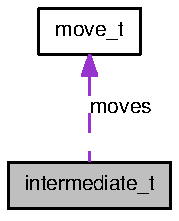
\includegraphics[width=122pt]{structintermediate__t__coll__graph}
\end{center}
\end{figure}


The documentation for this struct was generated from the following file:\begin{DoxyCompactItemize}
\item 
H/\hyperlink{data__structures_8h}{data\_\-structures.h}\end{DoxyCompactItemize}

\hypertarget{structINTERVAL}{
\section{INTERVAL Struct Reference}
\label{structINTERVAL}\index{INTERVAL@{INTERVAL}}
}


sequence interval stack element used in subopt.c  




\subsection{Detailed Description}
sequence interval stack element used in subopt.c 

The documentation for this struct was generated from the following file:\begin{DoxyCompactItemize}
\item 
H/\hyperlink{data__structures_8h}{data\_\-structures.h}\end{DoxyCompactItemize}

\hypertarget{structLIST}{
\section{LIST Struct Reference}
\label{structLIST}\index{LIST@{LIST}}
}


Collaboration diagram for LIST:\nopagebreak
\begin{figure}[H]
\begin{center}
\leavevmode
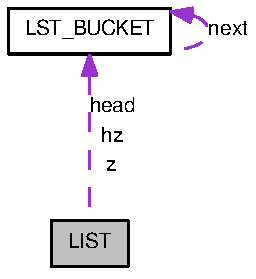
\includegraphics[width=159pt]{structLIST__coll__graph}
\end{center}
\end{figure}


The documentation for this struct was generated from the following file:\begin{DoxyCompactItemize}
\item 
lib/list.h\end{DoxyCompactItemize}

\hypertarget{structLST__BUCKET}{
\section{LST\_\-BUCKET Struct Reference}
\label{structLST__BUCKET}\index{LST\_\-BUCKET@{LST\_\-BUCKET}}
}


Collaboration diagram for LST\_\-BUCKET:\nopagebreak
\begin{figure}[H]
\begin{center}
\leavevmode
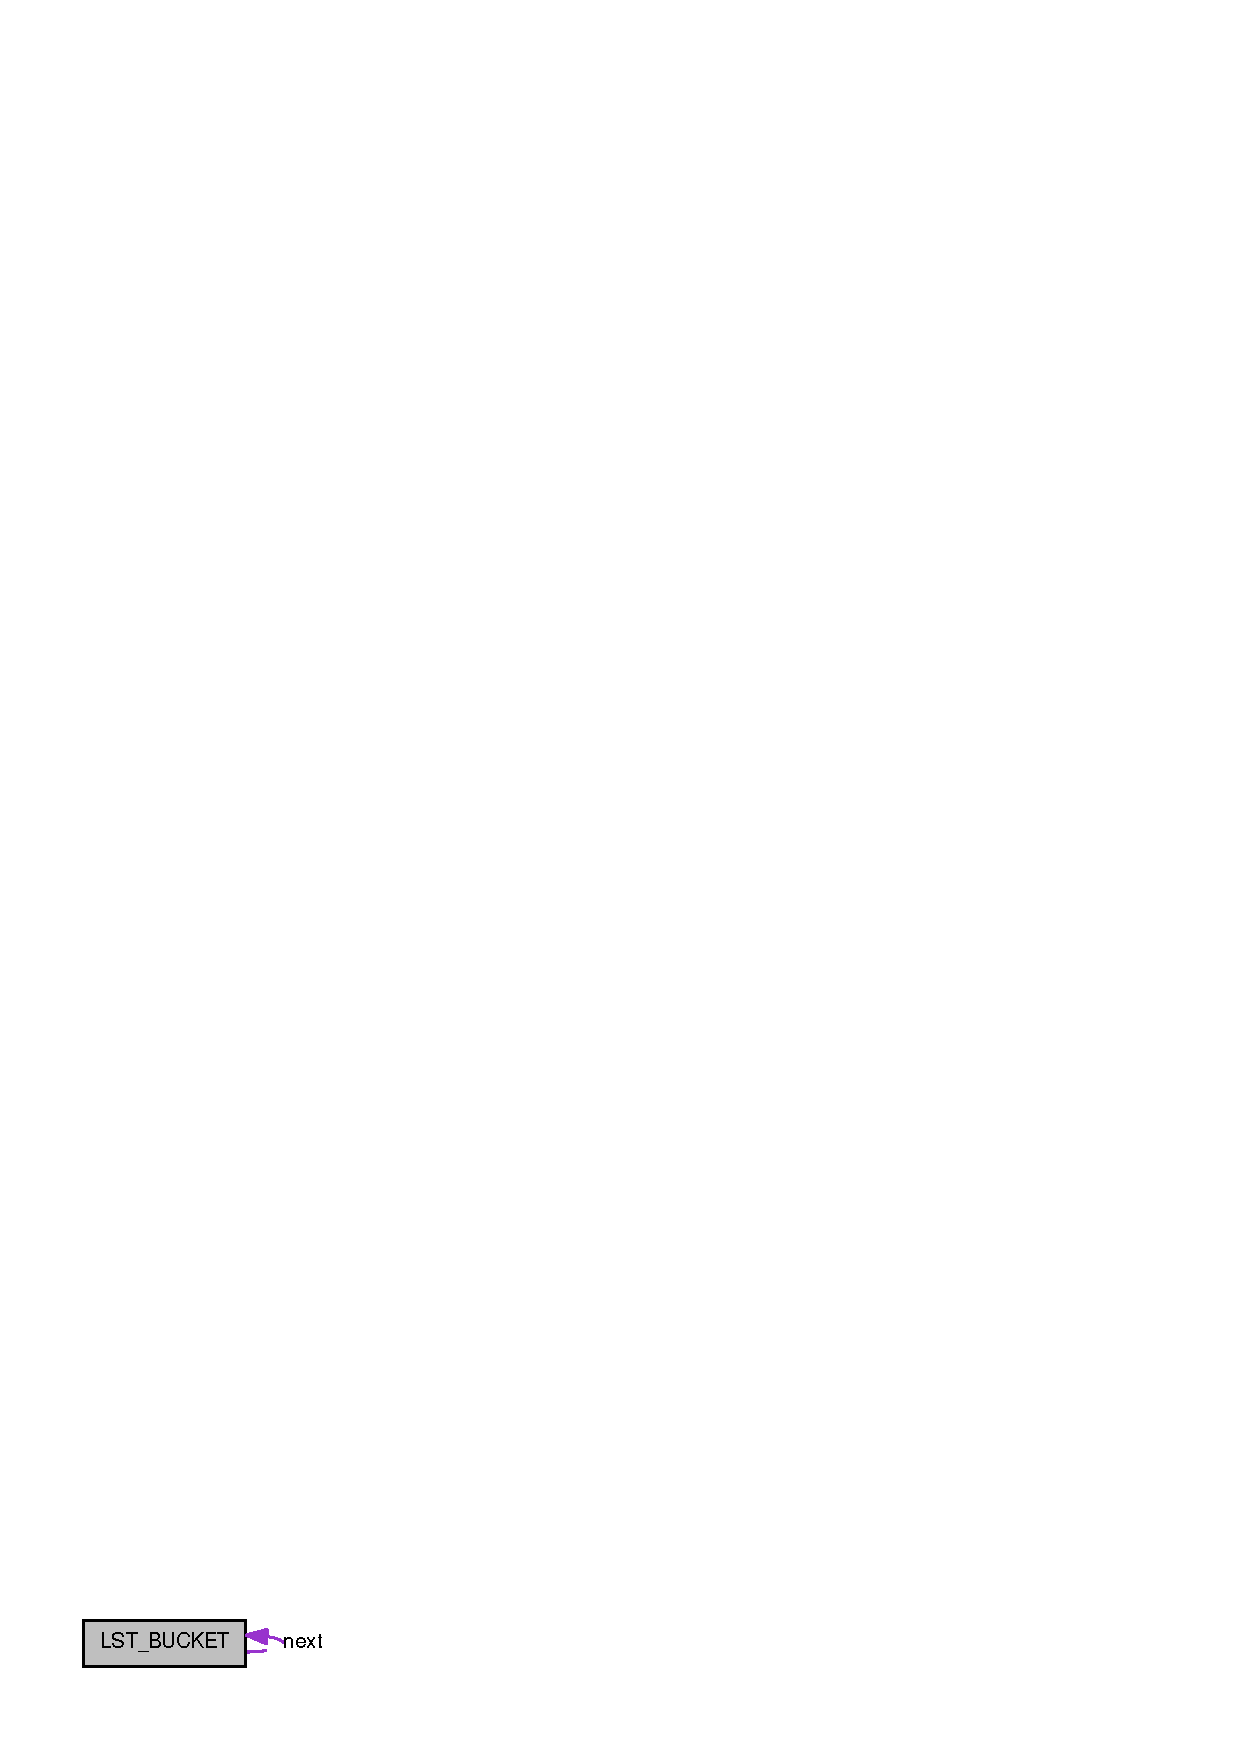
\includegraphics[width=159pt]{structLST__BUCKET__coll__graph}
\end{center}
\end{figure}


The documentation for this struct was generated from the following file:\begin{DoxyCompactItemize}
\item 
lib/list.h\end{DoxyCompactItemize}

\hypertarget{structmodel__detailsT}{
\section{model\_\-detailsT Struct Reference}
\label{structmodel__detailsT}\index{model\_\-detailsT@{model\_\-detailsT}}
}


The data structure that contains the complete model details used throughout the calculations.  




\subsection{Detailed Description}
The data structure that contains the complete model details used throughout the calculations. 

The documentation for this struct was generated from the following file:\begin{DoxyCompactItemize}
\item 
H/\hyperlink{data__structures_8h}{data\_\-structures.h}\end{DoxyCompactItemize}

\hypertarget{structmove__t}{
\section{move\_\-t Struct Reference}
\label{structmove__t}\index{move\_\-t@{move\_\-t}}
}


The documentation for this struct was generated from the following file:\begin{DoxyCompactItemize}
\item 
H/\hyperlink{data__structures_8h}{data\_\-structures.h}\end{DoxyCompactItemize}

\hypertarget{structPAIR}{
\section{PAIR Struct Reference}
\label{structPAIR}\index{PAIR@{PAIR}}
}


base pair data structure used in subopt.c  




\subsection{Detailed Description}
base pair data structure used in subopt.c 

The documentation for this struct was generated from the following file:\begin{DoxyCompactItemize}
\item 
H/\hyperlink{data__structures_8h}{data\_\-structures.h}\end{DoxyCompactItemize}

\hypertarget{structpair__info}{
\section{pair\_\-info Struct Reference}
\label{structpair__info}\index{pair\_\-info@{pair\_\-info}}
}


A base pair info structure.  




\subsection{Detailed Description}
A base pair info structure. for each base pair (i,j) the structure lists: its probability 'p', an entropy-\/like measure for its well-\/definedness 'ent', and in 'bp\mbox{[}\mbox{]}' the frequency of each type of pair. 'bp\mbox{[}0\mbox{]}' contains the number of non-\/compatible sequences, 'bp\mbox{[}1\mbox{]}' the number of CG pairs, etc. 

The documentation for this struct was generated from the following file:\begin{DoxyCompactItemize}
\item 
H/\hyperlink{data__structures_8h}{data\_\-structures.h}\end{DoxyCompactItemize}

\hypertarget{structpairpro}{
\section{pairpro Struct Reference}
\label{structpairpro}\index{pairpro@{pairpro}}
}


Collaboration diagram for pairpro:\nopagebreak
\begin{figure}[H]
\begin{center}
\leavevmode
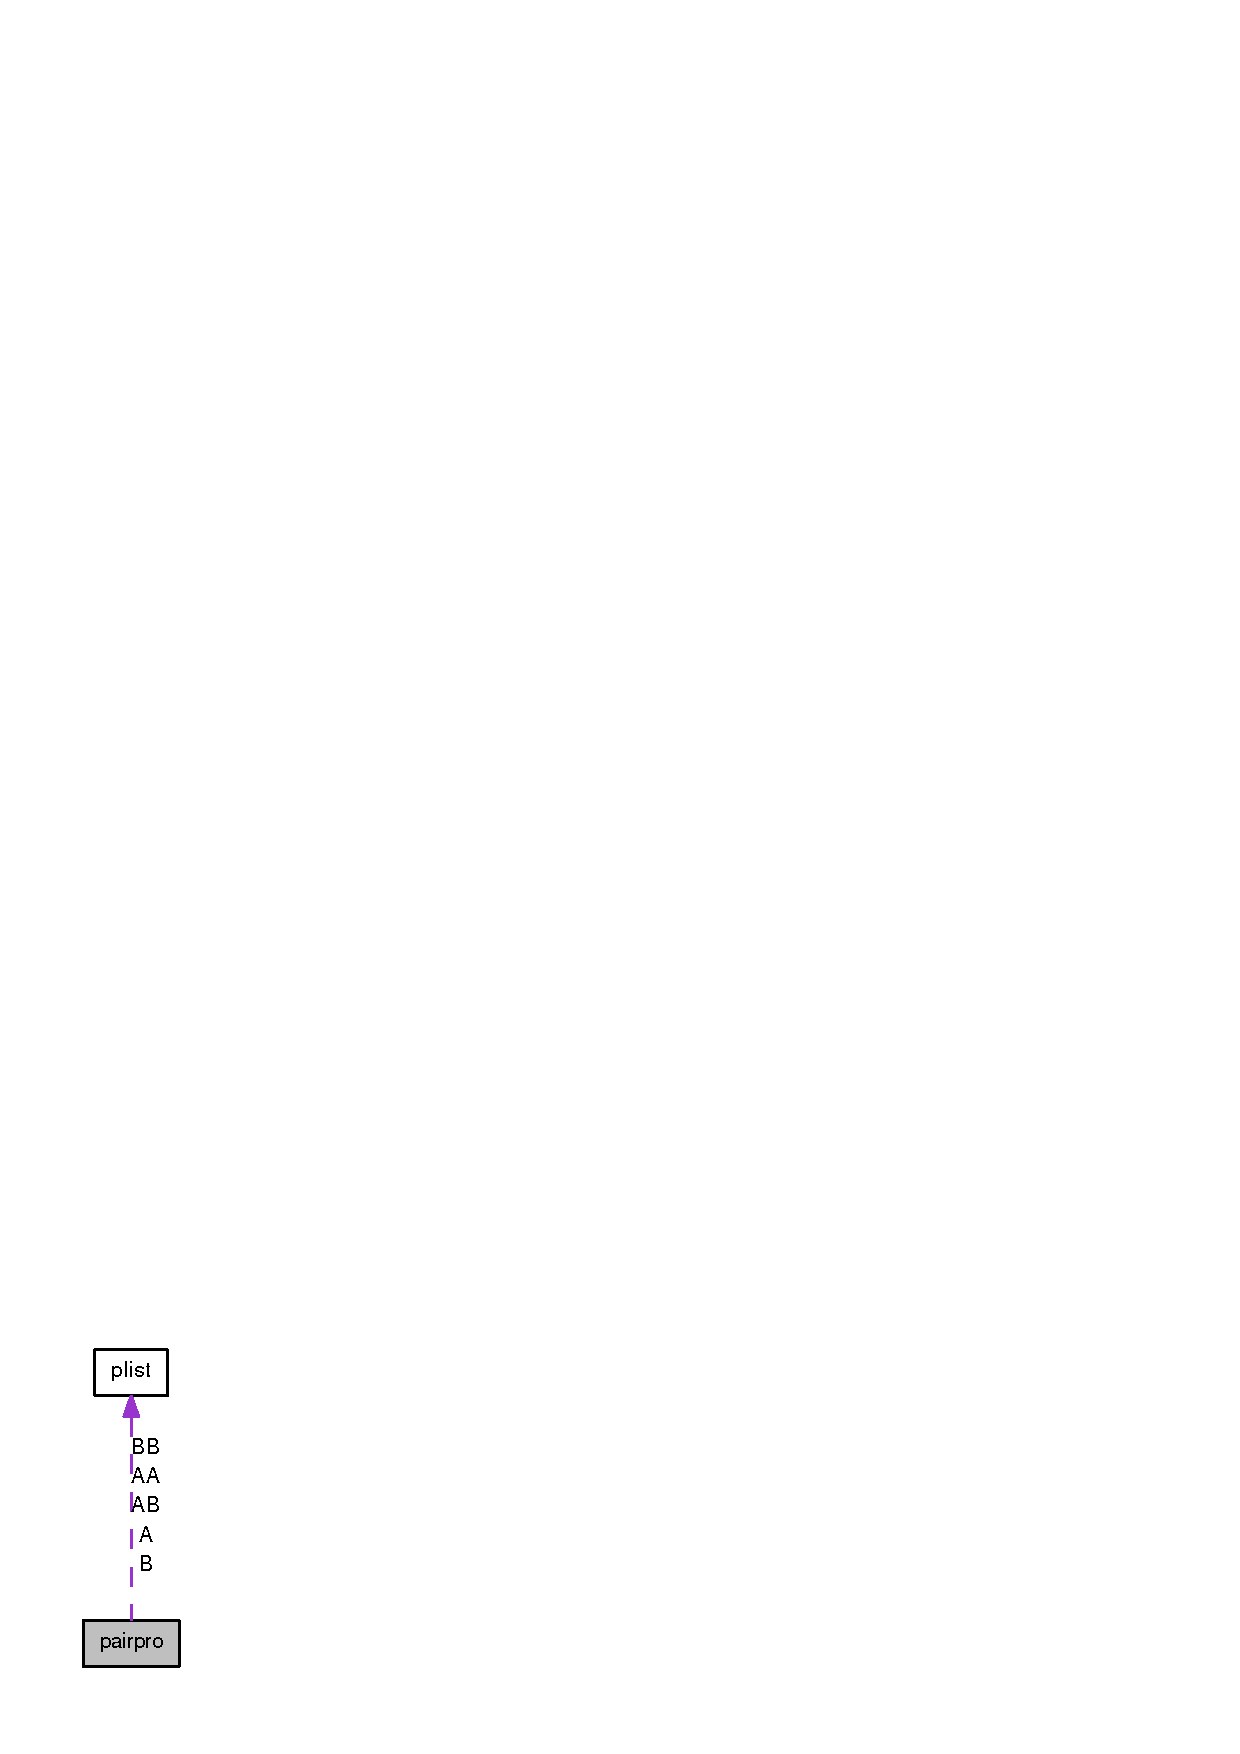
\includegraphics[width=90pt]{structpairpro__coll__graph}
\end{center}
\end{figure}


The documentation for this struct was generated from the following file:\begin{DoxyCompactItemize}
\item 
H/\hyperlink{data__structures_8h}{data\_\-structures.h}\end{DoxyCompactItemize}

\hypertarget{structparamT}{
\section{paramT Struct Reference}
\label{structparamT}\index{paramT@{paramT}}
}


The datastructure that contains temperature scaled energy parameters.  




Collaboration diagram for paramT:\nopagebreak
\begin{figure}[H]
\begin{center}
\leavevmode
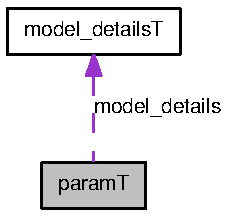
\includegraphics[width=146pt]{structparamT__coll__graph}
\end{center}
\end{figure}


\subsection{Detailed Description}
The datastructure that contains temperature scaled energy parameters. 

The documentation for this struct was generated from the following file:\begin{DoxyCompactItemize}
\item 
H/\hyperlink{data__structures_8h}{data\_\-structures.h}\end{DoxyCompactItemize}

\hypertarget{structpath__t}{
\section{path\_\-t Struct Reference}
\label{structpath__t}\index{path\_\-t@{path\_\-t}}
}


The documentation for this struct was generated from the following file:\begin{DoxyCompactItemize}
\item 
H/\hyperlink{data__structures_8h}{data\_\-structures.h}\end{DoxyCompactItemize}

\hypertarget{structpf__paramT}{
\section{pf\_\-paramT Struct Reference}
\label{structpf__paramT}\index{pf\_\-paramT@{pf\_\-paramT}}
}


The datastructure that contains temperature scaled Boltzmann weights of the energy parameters.  




Collaboration diagram for pf\_\-paramT:\nopagebreak
\begin{figure}[H]
\begin{center}
\leavevmode
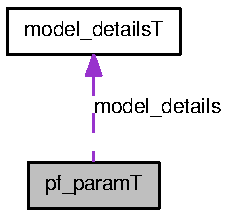
\includegraphics[width=146pt]{structpf__paramT__coll__graph}
\end{center}
\end{figure}


\subsection{Detailed Description}
The datastructure that contains temperature scaled Boltzmann weights of the energy parameters. 

The documentation for this struct was generated from the following file:\begin{DoxyCompactItemize}
\item 
H/\hyperlink{data__structures_8h}{data\_\-structures.h}\end{DoxyCompactItemize}

\hypertarget{structplist}{
\section{plist Struct Reference}
\label{structplist}\index{plist@{plist}}
}


this datastructure is used as input parameter in functions of \hyperlink{PS__dot_8h}{PS\_\-dot.h} and others  




\subsection{Detailed Description}
this datastructure is used as input parameter in functions of \hyperlink{PS__dot_8h}{PS\_\-dot.h} and others 

The documentation for this struct was generated from the following file:\begin{DoxyCompactItemize}
\item 
H/\hyperlink{data__structures_8h}{data\_\-structures.h}\end{DoxyCompactItemize}

\hypertarget{structPostorder__list}{
\section{Postorder\_\-list Struct Reference}
\label{structPostorder__list}\index{Postorder\_\-list@{Postorder\_\-list}}
}


The documentation for this struct was generated from the following file:\begin{DoxyCompactItemize}
\item 
H/\hyperlink{dist__vars_8h}{dist\_\-vars.h}\end{DoxyCompactItemize}

\hypertarget{structpu__contrib}{
\section{pu\_\-contrib Struct Reference}
\label{structpu__contrib}\index{pu\_\-contrib@{pu\_\-contrib}}
}


The documentation for this struct was generated from the following file:\begin{DoxyCompactItemize}
\item 
H/\hyperlink{data__structures_8h}{data\_\-structures.h}\end{DoxyCompactItemize}

\hypertarget{structpu__out}{
\section{pu\_\-out Struct Reference}
\label{structpu__out}\index{pu\_\-out@{pu\_\-out}}
}


The documentation for this struct was generated from the following file:\begin{DoxyCompactItemize}
\item 
H/\hyperlink{data__structures_8h}{data\_\-structures.h}\end{DoxyCompactItemize}

\hypertarget{structsect}{
\section{sect Struct Reference}
\label{structsect}\index{sect@{sect}}
}


stack of partial structures for backtracking  




\subsection{Detailed Description}
stack of partial structures for backtracking 

The documentation for this struct was generated from the following file:\begin{DoxyCompactItemize}
\item 
H/\hyperlink{data__structures_8h}{data\_\-structures.h}\end{DoxyCompactItemize}

\hypertarget{structsnoopT}{
\section{snoopT Struct Reference}
\label{structsnoopT}\index{snoopT@{snoopT}}
}


The documentation for this struct was generated from the following file:\begin{DoxyCompactItemize}
\item 
H/\hyperlink{data__structures_8h}{data\_\-structures.h}\end{DoxyCompactItemize}

\hypertarget{structSOLUTION}{
\section{SOLUTION Struct Reference}
\label{structSOLUTION}\index{SOLUTION@{SOLUTION}}
}


solution element from subopt.c  




\subsection{Detailed Description}
solution element from subopt.c 

The documentation for this struct was generated from the following file:\begin{DoxyCompactItemize}
\item 
H/\hyperlink{data__structures_8h}{data\_\-structures.h}\end{DoxyCompactItemize}

\hypertarget{structsvm__model}{
\section{svm\_\-model Struct Reference}
\label{structsvm__model}\index{svm\_\-model@{svm\_\-model}}
}


The documentation for this struct was generated from the following file:\begin{DoxyCompactItemize}
\item 
H/svm\_\-utils.h\end{DoxyCompactItemize}

\hypertarget{structswString}{
\section{swString Struct Reference}
\label{structswString}\index{swString@{swString}}
}


The documentation for this struct was generated from the following file:\begin{DoxyCompactItemize}
\item 
H/\hyperlink{dist__vars_8h}{dist\_\-vars.h}\end{DoxyCompactItemize}

\hypertarget{structTree}{
\section{Tree Struct Reference}
\label{structTree}\index{Tree@{Tree}}
}


Collaboration diagram for Tree:\nopagebreak
\begin{figure}[H]
\begin{center}
\leavevmode
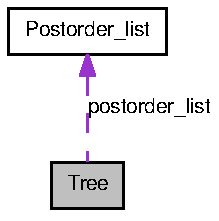
\includegraphics[width=141pt]{structTree__coll__graph}
\end{center}
\end{figure}


The documentation for this struct was generated from the following file:\begin{DoxyCompactItemize}
\item 
H/\hyperlink{dist__vars_8h}{dist\_\-vars.h}\end{DoxyCompactItemize}

\hypertarget{structTwoDfold__solution}{
\section{TwoDfold\_\-solution Struct Reference}
\label{structTwoDfold__solution}\index{TwoDfold\_\-solution@{TwoDfold\_\-solution}}
}


Solution element returned from TwoDfoldList.  




\subsection{Detailed Description}
Solution element returned from TwoDfoldList. This element contains free energy and structure for the appropriate kappa (k), lambda (l) neighborhood The datastructure contains two integer attributes 'k' and 'l' as well as an attribute 'en' of type float representing the free energy in kcal/mol and an attribute 's' of type char$\ast$ containg the secondary structure representative,

A value of \hyperlink{energy__const_8h_a12c2040f25d8e3a7b9e1c2024c618cb6}{INF} in k denotes the end of a list 

The documentation for this struct was generated from the following file:\begin{DoxyCompactItemize}
\item 
H/\hyperlink{data__structures_8h}{data\_\-structures.h}\end{DoxyCompactItemize}

\hypertarget{structTwoDfold__vars}{
\section{TwoDfold\_\-vars Struct Reference}
\label{structTwoDfold__vars}\index{TwoDfold\_\-vars@{TwoDfold\_\-vars}}
}


Variables compound for 2Dfold MFE folding.  




Collaboration diagram for TwoDfold\_\-vars:\nopagebreak
\begin{figure}[H]
\begin{center}
\leavevmode
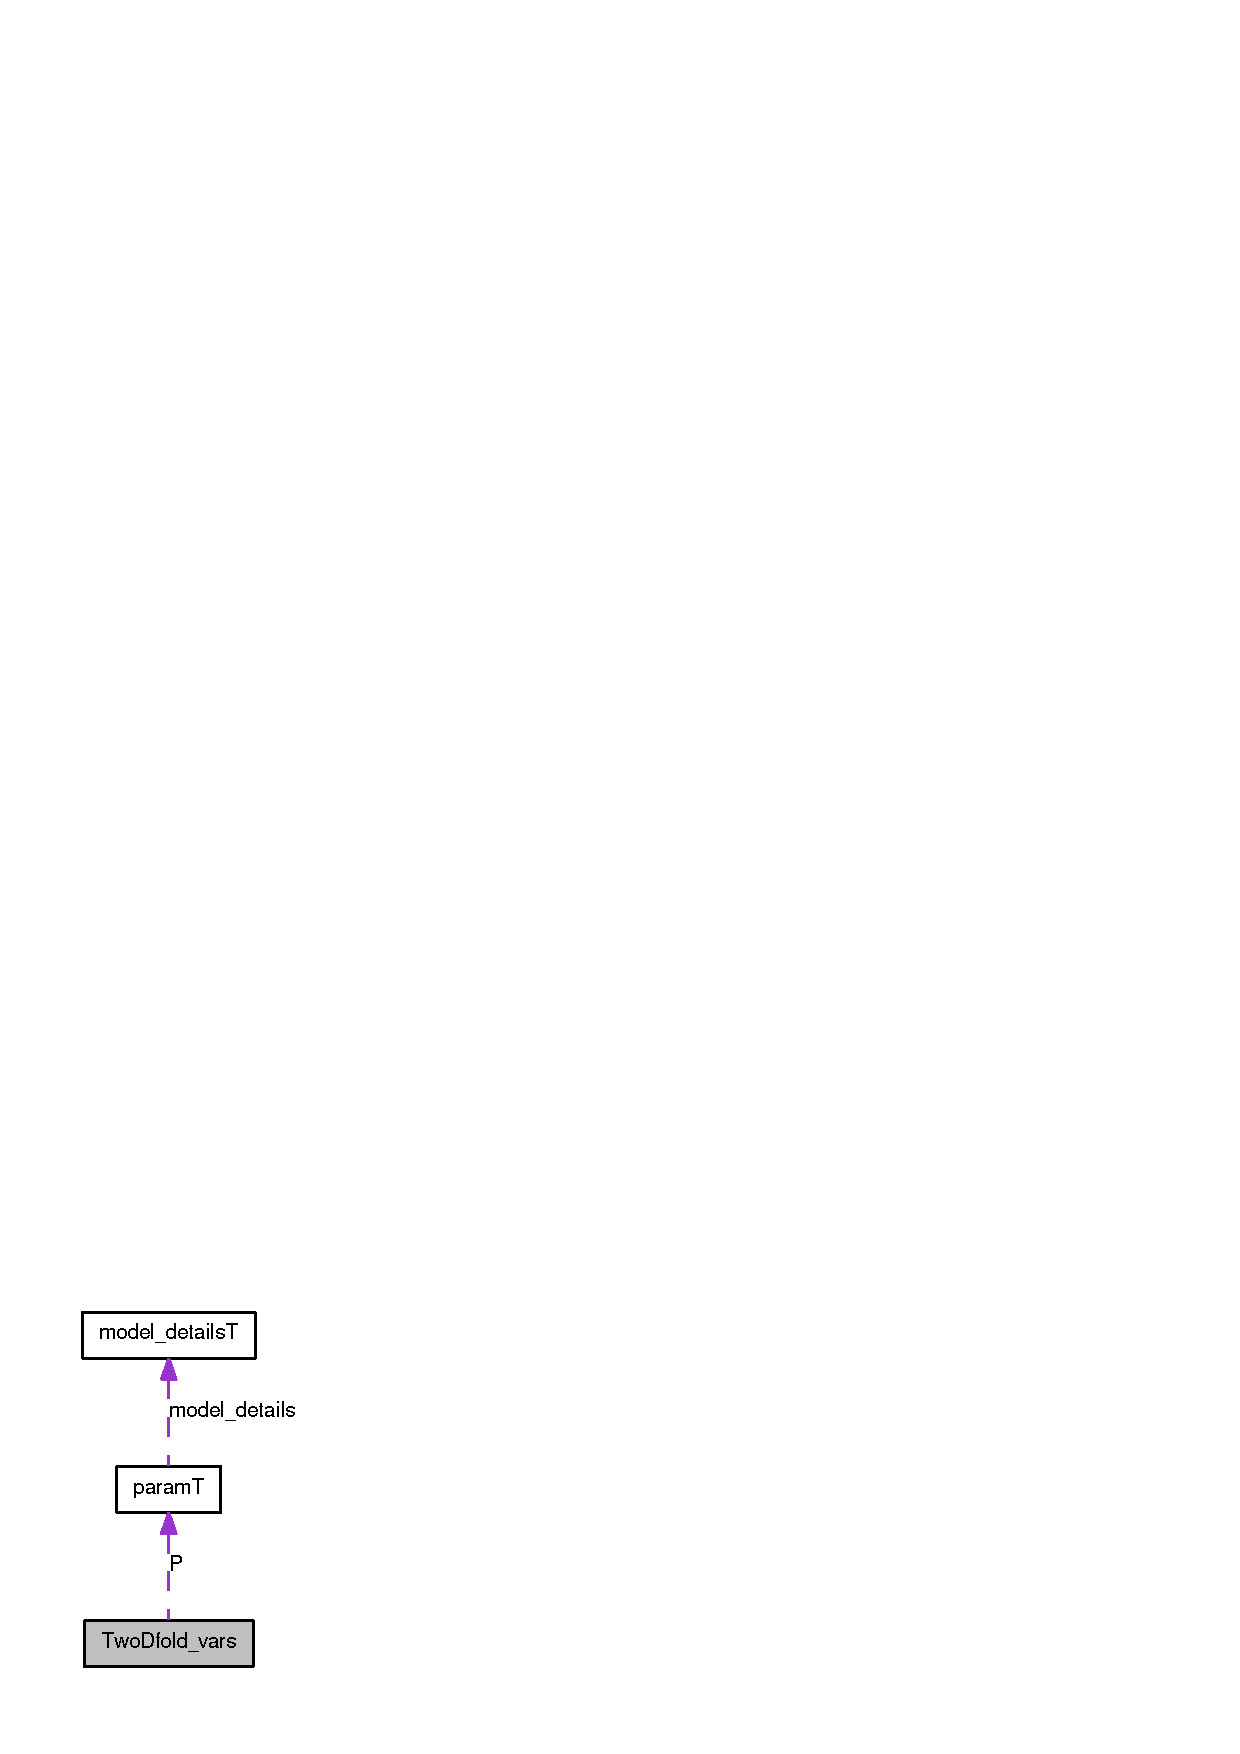
\includegraphics[width=146pt]{structTwoDfold__vars__coll__graph}
\end{center}
\end{figure}


\subsection{Detailed Description}
Variables compound for 2Dfold MFE folding. 

The documentation for this struct was generated from the following file:\begin{DoxyCompactItemize}
\item 
H/\hyperlink{data__structures_8h}{data\_\-structures.h}\end{DoxyCompactItemize}

\hypertarget{structTwoDpfold__solution}{
\section{TwoDpfold\_\-solution Struct Reference}
\label{structTwoDpfold__solution}\index{TwoDpfold\_\-solution@{TwoDpfold\_\-solution}}
}


Solution element returned from TwoDpfoldList.  




\subsection{Detailed Description}
Solution element returned from TwoDpfoldList. This element contains the partition function for the appropriate kappa (k), lambda (l) neighborhood The datastructure contains two integer attributes 'k' and 'l' as well as an attribute 'q' of type FLT\_\-OR\_\-DBL

A value of \hyperlink{energy__const_8h_a12c2040f25d8e3a7b9e1c2024c618cb6}{INF} in k denotes the end of a list 

The documentation for this struct was generated from the following file:\begin{DoxyCompactItemize}
\item 
H/\hyperlink{data__structures_8h}{data\_\-structures.h}\end{DoxyCompactItemize}

\hypertarget{structTwoDpfold__vars}{
\section{TwoDpfold\_\-vars Struct Reference}
\label{structTwoDpfold__vars}\index{TwoDpfold\_\-vars@{TwoDpfold\_\-vars}}
}


Variables compound for 2Dfold partition function folding.  




Collaboration diagram for TwoDpfold\_\-vars:\nopagebreak
\begin{figure}[H]
\begin{center}
\leavevmode
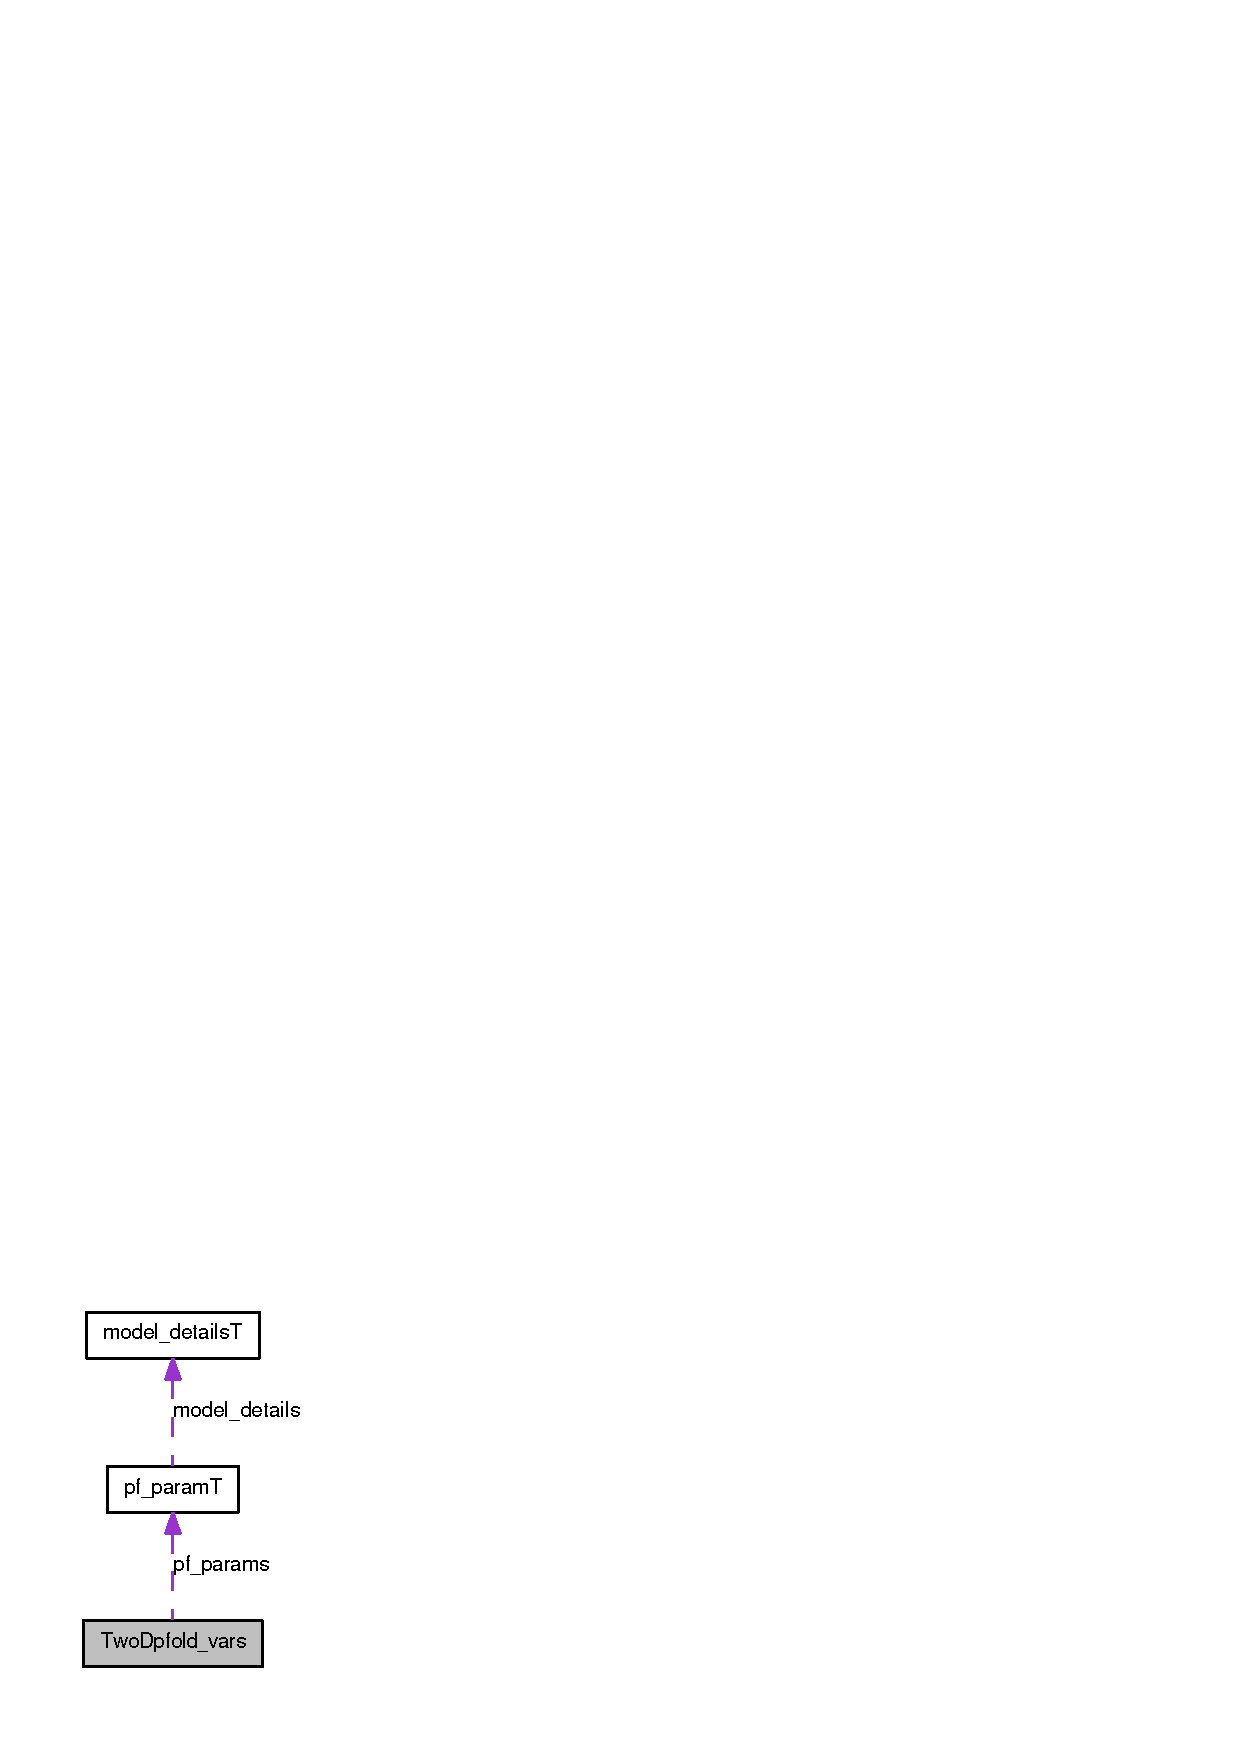
\includegraphics[width=148pt]{structTwoDpfold__vars__coll__graph}
\end{center}
\end{figure}


\subsection{Detailed Description}
Variables compound for 2Dfold partition function folding. 

The documentation for this struct was generated from the following file:\begin{DoxyCompactItemize}
\item 
H/\hyperlink{data__structures_8h}{data\_\-structures.h}\end{DoxyCompactItemize}

\chapter{File Documentation}
\hypertarget{2Dfold_8h}{
\section{H/2Dfold.h File Reference}
\label{2Dfold_8h}\index{H/2Dfold.h@{H/2Dfold.h}}
}


Compute the minimum free energy (MFE) and secondary structures for a partitioning of the secondary structure space according to the base pair distance to two fixed reference structures basepair distance to two fixed reference structures.  


Include dependency graph for 2Dfold.h:\nopagebreak
\begin{figure}[H]
\begin{center}
\leavevmode
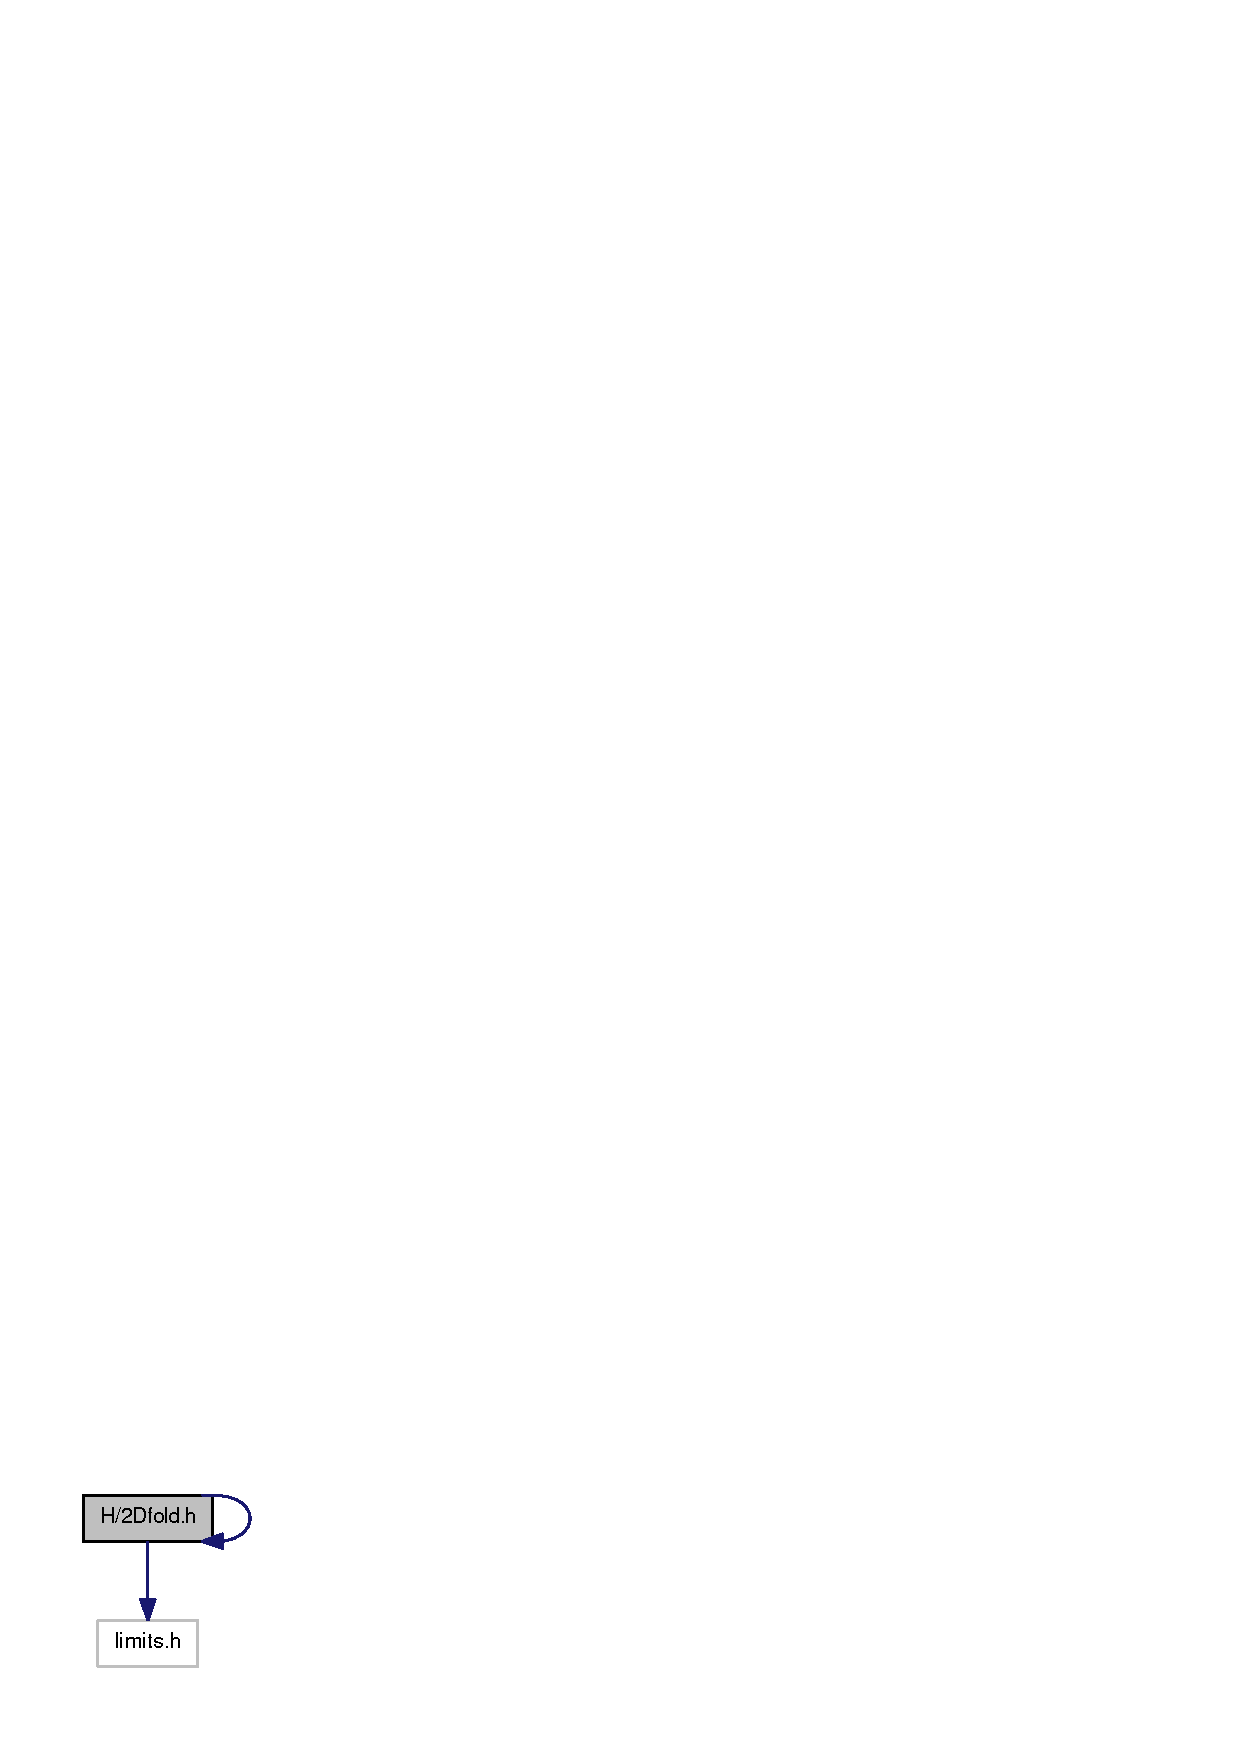
\includegraphics[width=62pt]{2Dfold_8h__incl}
\end{center}
\end{figure}
This graph shows which files directly or indirectly include this file:\nopagebreak
\begin{figure}[H]
\begin{center}
\leavevmode
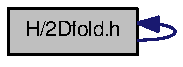
\includegraphics[width=62pt]{2Dfold_8h__dep__incl}
\end{center}
\end{figure}
\subsection*{Functions}
\begin{DoxyCompactItemize}
\item 
\hyperlink{structTwoDfold__vars}{TwoDfold\_\-vars} $\ast$ \hyperlink{2Dfold_8h_ac9284f132cf0eaa0a2f43590eda05488}{get\_\-TwoDfold\_\-variables} (const char $\ast$seq, const char $\ast$structure1, const char $\ast$structure2, int \hyperlink{fold__vars_8h_af9202a1a09f5828dc731e2d9a10fa111}{circ})
\begin{DoxyCompactList}\small\item\em Get a structure of type \hyperlink{structTwoDfold__vars}{TwoDfold\_\-vars} prefilled with current global settings. \item\end{DoxyCompactList}\item 
void \hyperlink{2Dfold_8h_a05bf4f31d216b1b160fd2d3d68e9b487}{destroy\_\-TwoDfold\_\-variables} (\hyperlink{structTwoDfold__vars}{TwoDfold\_\-vars} $\ast$our\_\-variables)
\begin{DoxyCompactList}\small\item\em Destroy a \hyperlink{structTwoDfold__vars}{TwoDfold\_\-vars} datastructure without memory loss. \item\end{DoxyCompactList}\item 
\hyperlink{structTwoDfold__solution}{TwoDfold\_\-solution} $\ast$ \hyperlink{2Dfold_8h_a47da790166020558d27323aef489703e}{TwoDfoldList} (\hyperlink{structTwoDfold__vars}{TwoDfold\_\-vars} $\ast$vars, int distance1, int distance2)
\begin{DoxyCompactList}\small\item\em Compute MFE's and representative for distance partitioning. \item\end{DoxyCompactList}\item 
char $\ast$ \hyperlink{2Dfold_8h_af4dc05bf8fc1ea53acd7aeb798ba80c2}{TwoDfold\_\-backtrack\_\-f5} (unsigned int j, int k, int l, \hyperlink{structTwoDfold__vars}{TwoDfold\_\-vars} $\ast$vars)
\begin{DoxyCompactList}\small\item\em Backtrack a minimum free energy structure from a 5' section of specified length. \item\end{DoxyCompactList}\end{DoxyCompactItemize}


\subsection{Detailed Description}
Compute the minimum free energy (MFE) and secondary structures for a partitioning of the secondary structure space according to the base pair distance to two fixed reference structures basepair distance to two fixed reference structures. 

\subsection{Function Documentation}
\hypertarget{2Dfold_8h_ac9284f132cf0eaa0a2f43590eda05488}{
\index{2Dfold.h@{2Dfold.h}!get\_\-TwoDfold\_\-variables@{get\_\-TwoDfold\_\-variables}}
\index{get\_\-TwoDfold\_\-variables@{get\_\-TwoDfold\_\-variables}!2Dfold.h@{2Dfold.h}}
\subsubsection[{get\_\-TwoDfold\_\-variables}]{\setlength{\rightskip}{0pt plus 5cm}{\bf TwoDfold\_\-vars}$\ast$ get\_\-TwoDfold\_\-variables (const char $\ast$ {\em seq}, \/  const char $\ast$ {\em structure1}, \/  const char $\ast$ {\em structure2}, \/  int {\em circ})}}
\label{2Dfold_8h_ac9284f132cf0eaa0a2f43590eda05488}


Get a structure of type \hyperlink{structTwoDfold__vars}{TwoDfold\_\-vars} prefilled with current global settings. 

This function returns a datastructure of type \hyperlink{structTwoDfold__vars}{TwoDfold\_\-vars}. The data fields inside the \hyperlink{structTwoDfold__vars}{TwoDfold\_\-vars} are prefilled by global settings and all memory allocations necessary to start a computation are already done for the convenience of the user

\begin{DoxyNote}{Note}
Make sure that the reference structures are compatible with the sequence according to Watson-\/Crick-\/ and Wobble-\/base pairing
\end{DoxyNote}
\begin{DoxySeeAlso}{See also}
\hyperlink{2Dfold_8h_a05bf4f31d216b1b160fd2d3d68e9b487}{destroy\_\-TwoDfold\_\-variables()}, TwoDfold(), TwoDfold\_\-circ
\end{DoxySeeAlso}

\begin{DoxyParams}{Parameters}
\item[{\em seq}]The RNA sequence 
\begin{DoxyParams}{Parameters}
\item[{\em structure1}]The first reference structure in dot-\/bracket notation 
\begin{DoxyParams}{Parameters}
\item[{\em structure2}]The second reference structure in dot-\/bracket notation 
\begin{DoxyParams}{Parameters}
\item[{\em circ}]A switch to indicate the assumption to fold a circular instead of linear RNA (0=OFF, 1=ON) \begin{DoxyReturn}{Returns}
A datastructure prefilled with folding options and allocated memory 
\end{DoxyReturn}
\end{DoxyParams}
\end{DoxyParams}
\end{DoxyParams}
\end{DoxyParams}
\hypertarget{2Dfold_8h_a05bf4f31d216b1b160fd2d3d68e9b487}{
\index{2Dfold.h@{2Dfold.h}!destroy\_\-TwoDfold\_\-variables@{destroy\_\-TwoDfold\_\-variables}}
\index{destroy\_\-TwoDfold\_\-variables@{destroy\_\-TwoDfold\_\-variables}!2Dfold.h@{2Dfold.h}}
\subsubsection[{destroy\_\-TwoDfold\_\-variables}]{\setlength{\rightskip}{0pt plus 5cm}void destroy\_\-TwoDfold\_\-variables ({\bf TwoDfold\_\-vars} $\ast$ {\em our\_\-variables})}}
\label{2Dfold_8h_a05bf4f31d216b1b160fd2d3d68e9b487}


Destroy a \hyperlink{structTwoDfold__vars}{TwoDfold\_\-vars} datastructure without memory loss. 

This function free's all allocated memory that depends on the datastructure given.

\begin{DoxySeeAlso}{See also}
\hyperlink{2Dfold_8h_ac9284f132cf0eaa0a2f43590eda05488}{get\_\-TwoDfold\_\-variables()}
\end{DoxySeeAlso}

\begin{DoxyParams}{Parameters}
\item[{\em our\_\-variables}]A pointer to the datastructure to be destroyed \end{DoxyParams}
\hypertarget{2Dfold_8h_a47da790166020558d27323aef489703e}{
\index{2Dfold.h@{2Dfold.h}!TwoDfoldList@{TwoDfoldList}}
\index{TwoDfoldList@{TwoDfoldList}!2Dfold.h@{2Dfold.h}}
\subsubsection[{TwoDfoldList}]{\setlength{\rightskip}{0pt plus 5cm}{\bf TwoDfold\_\-solution}$\ast$ TwoDfoldList ({\bf TwoDfold\_\-vars} $\ast$ {\em vars}, \/  int {\em distance1}, \/  int {\em distance2})}}
\label{2Dfold_8h_a47da790166020558d27323aef489703e}


Compute MFE's and representative for distance partitioning. 

This function computes the minimum free energies and a representative secondary structure for each distance class according to the two references specified in the datastructure 'vars'. The maximum basepair distance to each of both references may be set by the arguments 'distance1' and 'distance2', respectively. If both distance arguments are set to '-\/1', no restriction is assumed and the calculation is performed for each distance class possible.

The returned list contains an entry for each distance class. If a maximum basepair distance to either of the references was passed, an entry with k=l=-\/1 will be appended in the list, denoting the class where all structures exceeding the maximum will be thrown into. The end of the list is denoted by an attribute value of \hyperlink{energy__const_8h_a12c2040f25d8e3a7b9e1c2024c618cb6}{INF} in the k-\/attribute of the list entry.

\begin{DoxySeeAlso}{See also}
\hyperlink{2Dfold_8h_ac9284f132cf0eaa0a2f43590eda05488}{get\_\-TwoDfold\_\-variables()}, \hyperlink{2Dfold_8h_a05bf4f31d216b1b160fd2d3d68e9b487}{destroy\_\-TwoDfold\_\-variables()}, \hyperlink{structTwoDfold__solution}{TwoDfold\_\-solution}
\end{DoxySeeAlso}

\begin{DoxyParams}{Parameters}
\item[{\em vars}]the datastructure containing all predefined folding attributes 
\begin{DoxyParams}{Parameters}
\item[{\em distance1}]maximum distance to reference1 (-\/1 means no restriction) 
\begin{DoxyParams}{Parameters}
\item[{\em distance2}]maximum distance to reference2 (-\/1 means no restriction) \end{DoxyParams}
\end{DoxyParams}
\end{DoxyParams}
\hypertarget{2Dfold_8h_af4dc05bf8fc1ea53acd7aeb798ba80c2}{
\index{2Dfold.h@{2Dfold.h}!TwoDfold\_\-backtrack\_\-f5@{TwoDfold\_\-backtrack\_\-f5}}
\index{TwoDfold\_\-backtrack\_\-f5@{TwoDfold\_\-backtrack\_\-f5}!2Dfold.h@{2Dfold.h}}
\subsubsection[{TwoDfold\_\-backtrack\_\-f5}]{\setlength{\rightskip}{0pt plus 5cm}char$\ast$ TwoDfold\_\-backtrack\_\-f5 (unsigned int {\em j}, \/  int {\em k}, \/  int {\em l}, \/  {\bf TwoDfold\_\-vars} $\ast$ {\em vars})}}
\label{2Dfold_8h_af4dc05bf8fc1ea53acd7aeb798ba80c2}


Backtrack a minimum free energy structure from a 5' section of specified length. 

This function allows to backtrack a secondary structure beginning at the 5' end, a specified length and residing in a specific distance class. If the argument 'k' gets a value of -\/1, the structure that is backtracked is assumed to reside in the distance class where all structures exceeding the maximum basepair distance specified in \hyperlink{2Dfold_8h_a47da790166020558d27323aef489703e}{TwoDfoldList()} belong to. \begin{DoxyNote}{Note}
The argument 'vars' must contain precalculated energy values in the energy matrices, i.e. a call to \hyperlink{2Dfold_8h_a47da790166020558d27323aef489703e}{TwoDfoldList()} preceding this function is mandatory!
\end{DoxyNote}
\begin{DoxySeeAlso}{See also}
\hyperlink{2Dfold_8h_a47da790166020558d27323aef489703e}{TwoDfoldList()}, \hyperlink{2Dfold_8h_ac9284f132cf0eaa0a2f43590eda05488}{get\_\-TwoDfold\_\-variables()}, \hyperlink{2Dfold_8h_a05bf4f31d216b1b160fd2d3d68e9b487}{destroy\_\-TwoDfold\_\-variables()}
\end{DoxySeeAlso}

\begin{DoxyParams}{Parameters}
\item[{\em j}]The length in nucleotides beginning from the 5' end 
\begin{DoxyParams}{Parameters}
\item[{\em k}]distance to reference1 (may be -\/1) 
\begin{DoxyParams}{Parameters}
\item[{\em l}]distance to reference2 
\begin{DoxyParams}{Parameters}
\item[{\em vars}]the datastructure containing all predefined folding attributes \end{DoxyParams}
\end{DoxyParams}
\end{DoxyParams}
\end{DoxyParams}

\hypertarget{2Dpfold_8h}{
\section{H/2Dpfold.h File Reference}
\label{2Dpfold_8h}\index{H/2Dpfold.h@{H/2Dpfold.h}}
}


Compute the partition function and stochastically sample secondary structures for a partitioning of the secondary structure space according to the base pair distance to two fixed reference structures.  


Include dependency graph for 2Dpfold.h:\nopagebreak
\begin{figure}[H]
\begin{center}
\leavevmode
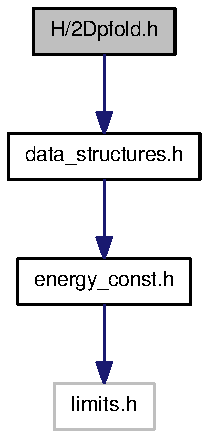
\includegraphics[width=68pt]{2Dpfold_8h__incl}
\end{center}
\end{figure}
\subsection*{Functions}
\begin{DoxyCompactItemize}
\item 
\hyperlink{structTwoDpfold__vars}{TwoDpfold\_\-vars} $\ast$ \hyperlink{2Dpfold_8h_a1aca740e2a75ab2b2951538266e53d64}{get\_\-TwoDpfold\_\-variables} (const char $\ast$seq, const char $\ast$structure1, char $\ast$structure2, int \hyperlink{fold__vars_8h_af9202a1a09f5828dc731e2d9a10fa111}{circ})
\begin{DoxyCompactList}\small\item\em Get a datastructure containing all necessary attributes and global folding switches. \item\end{DoxyCompactList}\item 
\hyperlink{structTwoDpfold__vars}{TwoDpfold\_\-vars} $\ast$ \hyperlink{2Dpfold_8h_acc2f66da7ee62096cab629fce7112216}{get\_\-TwoDpfold\_\-variables\_\-from\_\-MFE} (\hyperlink{structTwoDfold__vars}{TwoDfold\_\-vars} $\ast$mfe\_\-vars)
\begin{DoxyCompactList}\small\item\em Get the datastructure containing all necessary attributes and global folding switches from a pre-\/filled mfe-\/datastructure. \item\end{DoxyCompactList}\item 
void \hyperlink{2Dpfold_8h_afe994291458ee2ac34d3eb825ef62a15}{destroy\_\-TwoDpfold\_\-variables} (\hyperlink{structTwoDpfold__vars}{TwoDpfold\_\-vars} $\ast$vars)
\begin{DoxyCompactList}\small\item\em Free all memory occupied by a \hyperlink{structTwoDpfold__vars}{TwoDpfold\_\-vars} datastructure. \item\end{DoxyCompactList}\item 
\hyperlink{structTwoDpfold__solution}{TwoDpfold\_\-solution} $\ast$ \hyperlink{2Dpfold_8h_a3e1cd3b24eb635c65181182cbb4ae3eb}{TwoDpfoldList} (\hyperlink{structTwoDpfold__vars}{TwoDpfold\_\-vars} $\ast$vars, int maxDistance1, int maxDistance2)
\begin{DoxyCompactList}\small\item\em Compute the partition function for all distance classes. \item\end{DoxyCompactList}\item 
char $\ast$ \hyperlink{2Dpfold_8h_ae251288f50dd4ae7d315af0085775f71}{TwoDpfold\_\-pbacktrack} (\hyperlink{structTwoDpfold__vars}{TwoDpfold\_\-vars} $\ast$vars, int d1, int d2)
\begin{DoxyCompactList}\small\item\em Sample secondary structure representatives from a set of distance classes according to their Boltzmann probability. \item\end{DoxyCompactList}\item 
char $\ast$ \hyperlink{2Dpfold_8h_a13430ac6a7f90df426774f131647d2c7}{TwoDpfold\_\-pbacktrack5} (\hyperlink{structTwoDpfold__vars}{TwoDpfold\_\-vars} $\ast$vars, int d1, int d2, unsigned int length)
\begin{DoxyCompactList}\small\item\em Sample secondary structure representatives with a specified length from a set of distance classes according to their Boltzmann probability. \item\end{DoxyCompactList}\end{DoxyCompactItemize}


\subsection{Detailed Description}
Compute the partition function and stochastically sample secondary structures for a partitioning of the secondary structure space according to the base pair distance to two fixed reference structures. 

\subsection{Function Documentation}
\hypertarget{2Dpfold_8h_a1aca740e2a75ab2b2951538266e53d64}{
\index{2Dpfold.h@{2Dpfold.h}!get\_\-TwoDpfold\_\-variables@{get\_\-TwoDpfold\_\-variables}}
\index{get\_\-TwoDpfold\_\-variables@{get\_\-TwoDpfold\_\-variables}!2Dpfold.h@{2Dpfold.h}}
\subsubsection[{get\_\-TwoDpfold\_\-variables}]{\setlength{\rightskip}{0pt plus 5cm}{\bf TwoDpfold\_\-vars}$\ast$ get\_\-TwoDpfold\_\-variables (const char $\ast$ {\em seq}, \/  const char $\ast$ {\em structure1}, \/  char $\ast$ {\em structure2}, \/  int {\em circ})}}
\label{2Dpfold_8h_a1aca740e2a75ab2b2951538266e53d64}


Get a datastructure containing all necessary attributes and global folding switches. 

This function prepares all necessary attributes and matrices etc which are needed for a call of TwoDpfoldList. A snapshot of all current global model switches (dangles, temperature and so on) is done and stored in the returned datastructure. Additionally, all matrices that will hold the partition function values are prepared.


\begin{DoxyParams}{Parameters}
\item[{\em seq}]the RNA sequence in uppercase format with letters from the alphabet \{AUCG\} 
\begin{DoxyParams}{Parameters}
\item[{\em structure1}]the first reference structure in dot-\/bracket notation 
\begin{DoxyParams}{Parameters}
\item[{\em structure2}]the second reference structure in dot-\/bracket notation 
\begin{DoxyParams}{Parameters}
\item[{\em circ}]a switch indicating if the sequence is linear (0) or circular (1) \begin{DoxyReturn}{Returns}
the datastructure containing all necessary partition function attributes 
\end{DoxyReturn}
\end{DoxyParams}
\end{DoxyParams}
\end{DoxyParams}
\end{DoxyParams}
\hypertarget{2Dpfold_8h_acc2f66da7ee62096cab629fce7112216}{
\index{2Dpfold.h@{2Dpfold.h}!get\_\-TwoDpfold\_\-variables\_\-from\_\-MFE@{get\_\-TwoDpfold\_\-variables\_\-from\_\-MFE}}
\index{get\_\-TwoDpfold\_\-variables\_\-from\_\-MFE@{get\_\-TwoDpfold\_\-variables\_\-from\_\-MFE}!2Dpfold.h@{2Dpfold.h}}
\subsubsection[{get\_\-TwoDpfold\_\-variables\_\-from\_\-MFE}]{\setlength{\rightskip}{0pt plus 5cm}{\bf TwoDpfold\_\-vars}$\ast$ get\_\-TwoDpfold\_\-variables\_\-from\_\-MFE ({\bf TwoDfold\_\-vars} $\ast$ {\em mfe\_\-vars})}}
\label{2Dpfold_8h_acc2f66da7ee62096cab629fce7112216}


Get the datastructure containing all necessary attributes and global folding switches from a pre-\/filled mfe-\/datastructure. 

This function actually does the same as get\_\-TwoDpfold\_\-variables but takes its switches and settings from a pre-\/filled MFE equivalent datastructure

\begin{DoxySeeAlso}{See also}
\hyperlink{2Dfold_8h_ac9284f132cf0eaa0a2f43590eda05488}{get\_\-TwoDfold\_\-variables()}, \hyperlink{2Dpfold_8h_a1aca740e2a75ab2b2951538266e53d64}{get\_\-TwoDpfold\_\-variables()}
\end{DoxySeeAlso}

\begin{DoxyParams}{Parameters}
\item[{\em mfe\_\-vars}]the pre-\/filled mfe datastructure \begin{DoxyReturn}{Returns}
the datastructure containing all necessary partition function attributes 
\end{DoxyReturn}
\end{DoxyParams}
\hypertarget{2Dpfold_8h_afe994291458ee2ac34d3eb825ef62a15}{
\index{2Dpfold.h@{2Dpfold.h}!destroy\_\-TwoDpfold\_\-variables@{destroy\_\-TwoDpfold\_\-variables}}
\index{destroy\_\-TwoDpfold\_\-variables@{destroy\_\-TwoDpfold\_\-variables}!2Dpfold.h@{2Dpfold.h}}
\subsubsection[{destroy\_\-TwoDpfold\_\-variables}]{\setlength{\rightskip}{0pt plus 5cm}void destroy\_\-TwoDpfold\_\-variables ({\bf TwoDpfold\_\-vars} $\ast$ {\em vars})}}
\label{2Dpfold_8h_afe994291458ee2ac34d3eb825ef62a15}


Free all memory occupied by a \hyperlink{structTwoDpfold__vars}{TwoDpfold\_\-vars} datastructure. 

This function free's all memory occupied by a datastructure obtained from from \hyperlink{2Dpfold_8h_a1aca740e2a75ab2b2951538266e53d64}{get\_\-TwoDpfold\_\-variables()} or \hyperlink{2Dpfold_8h_acc2f66da7ee62096cab629fce7112216}{get\_\-TwoDpfold\_\-variables\_\-from\_\-MFE()}

\begin{DoxySeeAlso}{See also}
\hyperlink{2Dpfold_8h_a1aca740e2a75ab2b2951538266e53d64}{get\_\-TwoDpfold\_\-variables()}, \hyperlink{2Dpfold_8h_acc2f66da7ee62096cab629fce7112216}{get\_\-TwoDpfold\_\-variables\_\-from\_\-MFE()}
\end{DoxySeeAlso}

\begin{DoxyParams}{Parameters}
\item[{\em vars}]the datastructure to be free'd \end{DoxyParams}
\hypertarget{2Dpfold_8h_a3e1cd3b24eb635c65181182cbb4ae3eb}{
\index{2Dpfold.h@{2Dpfold.h}!TwoDpfoldList@{TwoDpfoldList}}
\index{TwoDpfoldList@{TwoDpfoldList}!2Dpfold.h@{2Dpfold.h}}
\subsubsection[{TwoDpfoldList}]{\setlength{\rightskip}{0pt plus 5cm}{\bf TwoDpfold\_\-solution}$\ast$ TwoDpfoldList ({\bf TwoDpfold\_\-vars} $\ast$ {\em vars}, \/  int {\em maxDistance1}, \/  int {\em maxDistance2})}}
\label{2Dpfold_8h_a3e1cd3b24eb635c65181182cbb4ae3eb}


Compute the partition function for all distance classes. 

This function computes the partition functions for all distance classes according the two reference structures specified in the datastructure 'vars'. Similar to \hyperlink{2Dfold_8h_a47da790166020558d27323aef489703e}{TwoDfoldList()} the arguments maxDistance1 and maxDistance2 specify the maximum distance to both reference structures. A value of '-\/1' in either of them makes the appropriate distance restrictionless, i.e. all basepair distancies to the reference are taken into account during computation. In case there is a restriction, the returned solution contains an entry where the attribute k=l=-\/1 contains the partition function for all structures exceeding the restriction. A values of \hyperlink{energy__const_8h_a12c2040f25d8e3a7b9e1c2024c618cb6}{INF} in the attribute 'k' of the returned list denotes the end of the list

\begin{DoxySeeAlso}{See also}
\hyperlink{2Dpfold_8h_a1aca740e2a75ab2b2951538266e53d64}{get\_\-TwoDpfold\_\-variables()}, \hyperlink{2Dpfold_8h_afe994291458ee2ac34d3eb825ef62a15}{destroy\_\-TwoDpfold\_\-variables()}, \hyperlink{structTwoDpfold__solution}{TwoDpfold\_\-solution}
\end{DoxySeeAlso}

\begin{DoxyParams}{Parameters}
\item[{\em vars}]the datastructure containing all necessary folding attributes and matrices 
\begin{DoxyParams}{Parameters}
\item[{\em maxDistance1}]the maximum basepair distance to reference1 (may be -\/1) 
\begin{DoxyParams}{Parameters}
\item[{\em maxDistance2}]the maximum basepair distance to reference2 (may be -\/1) \begin{DoxyReturn}{Returns}
a list of partition funtions for the appropriate distance classes 
\end{DoxyReturn}
\end{DoxyParams}
\end{DoxyParams}
\end{DoxyParams}
\hypertarget{2Dpfold_8h_ae251288f50dd4ae7d315af0085775f71}{
\index{2Dpfold.h@{2Dpfold.h}!TwoDpfold\_\-pbacktrack@{TwoDpfold\_\-pbacktrack}}
\index{TwoDpfold\_\-pbacktrack@{TwoDpfold\_\-pbacktrack}!2Dpfold.h@{2Dpfold.h}}
\subsubsection[{TwoDpfold\_\-pbacktrack}]{\setlength{\rightskip}{0pt plus 5cm}char$\ast$ TwoDpfold\_\-pbacktrack ({\bf TwoDpfold\_\-vars} $\ast$ {\em vars}, \/  int {\em d1}, \/  int {\em d2})}}
\label{2Dpfold_8h_ae251288f50dd4ae7d315af0085775f71}


Sample secondary structure representatives from a set of distance classes according to their Boltzmann probability. 

If the argument 'd1' is set to '-\/1', the structure will be backtracked in the distance class where all structures exceeding the maximum basepair distance to either of the references reside.

\begin{DoxyNote}{Note}
The argument 'vars' must contain precalculated partition function matrices, i.e. a call to \hyperlink{2Dpfold_8h_a3e1cd3b24eb635c65181182cbb4ae3eb}{TwoDpfoldList()} preceding this function is mandatory!
\end{DoxyNote}
\begin{DoxySeeAlso}{See also}
\hyperlink{2Dpfold_8h_a3e1cd3b24eb635c65181182cbb4ae3eb}{TwoDpfoldList()}
\end{DoxySeeAlso}

\begin{DoxyParams}{Parameters}
\item[{\em vars}]the datastructure containing all necessary folding attributes and matrices 
\begin{DoxyParams}{Parameters}
\item[{\em d1}]the distance to reference1 (may be -\/1) 
\begin{DoxyParams}{Parameters}
\item[{\em d2}]the distance to reference2 \begin{DoxyReturn}{Returns}
a sampled secondary structure in dot-\/bracket notation 
\end{DoxyReturn}
\end{DoxyParams}
\end{DoxyParams}
\end{DoxyParams}
\hypertarget{2Dpfold_8h_a13430ac6a7f90df426774f131647d2c7}{
\index{2Dpfold.h@{2Dpfold.h}!TwoDpfold\_\-pbacktrack5@{TwoDpfold\_\-pbacktrack5}}
\index{TwoDpfold\_\-pbacktrack5@{TwoDpfold\_\-pbacktrack5}!2Dpfold.h@{2Dpfold.h}}
\subsubsection[{TwoDpfold\_\-pbacktrack5}]{\setlength{\rightskip}{0pt plus 5cm}char$\ast$ TwoDpfold\_\-pbacktrack5 ({\bf TwoDpfold\_\-vars} $\ast$ {\em vars}, \/  int {\em d1}, \/  int {\em d2}, \/  unsigned int {\em length})}}
\label{2Dpfold_8h_a13430ac6a7f90df426774f131647d2c7}


Sample secondary structure representatives with a specified length from a set of distance classes according to their Boltzmann probability. 

This function does essentially the same as TwoDpfold\_\-pbacktrack with the only difference that partial structures, i.e. structures beginning from the 5' end with a specified length of the sequence, are backtracked

\begin{DoxyNote}{Note}
The argument 'vars' must contain precalculated partition function matrices, i.e. a call to \hyperlink{2Dpfold_8h_a3e1cd3b24eb635c65181182cbb4ae3eb}{TwoDpfoldList()} preceding this function is mandatory! 

This function does not work (since it makes no sense) for circular RNA sequences!
\end{DoxyNote}
\begin{DoxySeeAlso}{See also}
\hyperlink{2Dpfold_8h_ae251288f50dd4ae7d315af0085775f71}{TwoDpfold\_\-pbacktrack()}, \hyperlink{2Dpfold_8h_a3e1cd3b24eb635c65181182cbb4ae3eb}{TwoDpfoldList()}
\end{DoxySeeAlso}

\begin{DoxyParams}{Parameters}
\item[{\em vars}]the datastructure containing all necessary folding attributes and matrices 
\begin{DoxyParams}{Parameters}
\item[{\em d1}]the distance to reference1 (may be -\/1) 
\begin{DoxyParams}{Parameters}
\item[{\em d2}]the distance to reference2 
\begin{DoxyParams}{Parameters}
\item[{\em length}]the length of the structure beginning from the 5' end \begin{DoxyReturn}{Returns}
a sampled secondary structure in dot-\/bracket notation 
\end{DoxyReturn}
\end{DoxyParams}
\end{DoxyParams}
\end{DoxyParams}
\end{DoxyParams}

\hypertarget{alifold_8h}{
\section{H/alifold.h File Reference}
\label{alifold_8h}\index{H/alifold.h@{H/alifold.h}}
}


compute various properties (consensus MFE structures, partition function, Boltzmann distributed stochastic samples, .  


Include dependency graph for alifold.h:\nopagebreak
\begin{figure}[H]
\begin{center}
\leavevmode
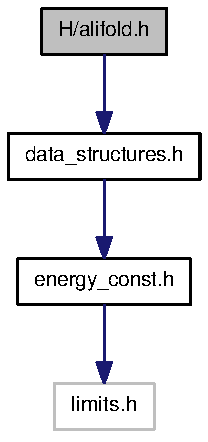
\includegraphics[width=68pt]{alifold_8h__incl}
\end{center}
\end{figure}
\subsection*{Functions}
\begin{DoxyCompactItemize}
\item 
void \hyperlink{alifold_8h_ac484c6bd429bafbd353b91044508d8e9}{update\_\-alifold\_\-params} (void)
\begin{DoxyCompactList}\small\item\em Update the energy parameters for alifold function. \item\end{DoxyCompactList}\item 
float \hyperlink{alifold_8h_a4cf00f0659e5f0480335d69e797f05b1}{alifold} (const char $\ast$$\ast$strings, char $\ast$structure)
\begin{DoxyCompactList}\small\item\em Compute MFE and according consensus structure of an alignment of sequences. \item\end{DoxyCompactList}\item 
float \hyperlink{alifold_8h_adbd3b0b1c144cbfb4efe704b2b260f96}{circalifold} (const char $\ast$$\ast$strings, char $\ast$structure)
\begin{DoxyCompactList}\small\item\em Compute MFE and according structure of an alignment of sequences assuming the sequences are circular instead of linear. \item\end{DoxyCompactList}\item 
\hypertarget{alifold_8h_a72095e4554b5d577250ea14c42acc49e}{
void \hyperlink{alifold_8h_a72095e4554b5d577250ea14c42acc49e}{free\_\-alifold\_\-arrays} (void)}
\label{alifold_8h_a72095e4554b5d577250ea14c42acc49e}

\begin{DoxyCompactList}\small\item\em Free the memory occupied by MFE alifold functions. \item\end{DoxyCompactList}\item 
int \hyperlink{alifold_8h_aa2d600be90844094ec145ea14a314d2f}{get\_\-mpi} (char $\ast$Alseq\mbox{[}$\,$\mbox{]}, int n\_\-seq, int length, int $\ast$mini)
\begin{DoxyCompactList}\small\item\em Get the mean pairwise identity in steps from ?to?(ident). \item\end{DoxyCompactList}\item 
\hypertarget{alifold_8h_a5e125c9586fcd4e2e1559fe76f7289cc}{
float $\ast$$\ast$ \hyperlink{alifold_8h_a5e125c9586fcd4e2e1559fe76f7289cc}{readribosum} (char $\ast$name)}
\label{alifold_8h_a5e125c9586fcd4e2e1559fe76f7289cc}

\begin{DoxyCompactList}\small\item\em Read a ribosum or other user-\/defined scoring matrix. \item\end{DoxyCompactList}\item 
float \hyperlink{alifold_8h_a1c48869c03b49a342bf4cbdd61900081}{energy\_\-of\_\-alistruct} (const char $\ast$$\ast$sequences, const char $\ast$structure, int n\_\-seq, float $\ast$energy)
\begin{DoxyCompactList}\small\item\em Calculate the free energy of a consensus structure given a set of aligned sequences. \item\end{DoxyCompactList}\item 
void \hyperlink{alifold_8h_aa3e40277c837d6f7603afe319884c786}{encode\_\-ali\_\-sequence} (const char $\ast$sequence, short $\ast$S, short $\ast$s5, short $\ast$s3, char $\ast$ss, unsigned short $\ast$as, int \hyperlink{fold__vars_8h_af9202a1a09f5828dc731e2d9a10fa111}{circ})
\begin{DoxyCompactList}\small\item\em Get arrays with encoded sequence of the alignment. \item\end{DoxyCompactList}\item 
void \hyperlink{alifold_8h_a8a560930f7f2582cc3967723a86cfdfa}{alloc\_\-sequence\_\-arrays} (const char $\ast$$\ast$sequences, short $\ast$$\ast$$\ast$S, short $\ast$$\ast$$\ast$S5, short $\ast$$\ast$$\ast$S3, unsigned short $\ast$$\ast$$\ast$a2s, char $\ast$$\ast$$\ast$Ss, int \hyperlink{fold__vars_8h_af9202a1a09f5828dc731e2d9a10fa111}{circ})
\begin{DoxyCompactList}\small\item\em Allocate memory for sequence array used to deal with aligned sequences. \item\end{DoxyCompactList}\item 
void \hyperlink{alifold_8h_a298a420a8c879202e2617b3f724fde38}{free\_\-sequence\_\-arrays} (unsigned int n\_\-seq, short $\ast$$\ast$$\ast$S, short $\ast$$\ast$$\ast$S5, short $\ast$$\ast$$\ast$S3, unsigned short $\ast$$\ast$$\ast$a2s, char $\ast$$\ast$$\ast$Ss)
\begin{DoxyCompactList}\small\item\em Free the memory of the sequence arrays used to deal with aligned sequences. \item\end{DoxyCompactList}\item 
float \hyperlink{alifold_8h_a4d2ff54d8210fc7cceeeff389d4dbd1d}{alipf\_\-fold\_\-par} (const char $\ast$$\ast$sequences, char $\ast$structure, \hyperlink{structplist}{plist} $\ast$$\ast$pl, \hyperlink{structpf__paramT}{pf\_\-paramT} $\ast$parameters, int calculate\_\-bppm, int is\_\-constrained, int is\_\-circular)
\item 
float \hyperlink{alifold_8h_ad32ded7d753ccaf211ab35782d1f42a9}{alipf\_\-fold} (const char $\ast$$\ast$sequences, char $\ast$structure, \hyperlink{structplist}{plist} $\ast$$\ast$pl)
\begin{DoxyCompactList}\small\item\em The partition function version of \hyperlink{alifold_8h_a4cf00f0659e5f0480335d69e797f05b1}{alifold()} works in analogy to \hyperlink{part__func_8h_adc3db3d98742427e7001a7fd36ef28c2}{pf\_\-fold()}. \item\end{DoxyCompactList}\item 
float \hyperlink{alifold_8h_a6b4dde1d43b79ab3753508c46cf50363}{alipf\_\-circ\_\-fold} (const char $\ast$$\ast$sequences, char $\ast$structure, \hyperlink{structplist}{plist} $\ast$$\ast$pl)
\item 
FLT\_\-OR\_\-DBL $\ast$ \hyperlink{alifold_8h_a11b6ab8bd9be1821fea352b190a01cab}{export\_\-ali\_\-bppm} (void)
\begin{DoxyCompactList}\small\item\em Get a pointer to the base pair probability array. \item\end{DoxyCompactList}\item 
char $\ast$ \hyperlink{alifold_8h_a0df40248788f0fb17ebdc59d74116d1c}{alipbacktrack} (double $\ast$prob)
\begin{DoxyCompactList}\small\item\em Sample a consensus secondary structure from the Boltzmann ensemble according its probability\par
. \item\end{DoxyCompactList}\end{DoxyCompactItemize}
\subsection*{Variables}
\begin{DoxyCompactItemize}
\item 
double \hyperlink{alifold_8h_af3cbac6ff5d706d6e414677841ddf94c}{cv\_\-fact}
\begin{DoxyCompactList}\small\item\em This variable controls the weight of the covariance term in the energy function of alignment folding algorithms. \item\end{DoxyCompactList}\item 
double \hyperlink{alifold_8h_a502948a122a2af5b914355b1f3ea2f61}{nc\_\-fact}
\begin{DoxyCompactList}\small\item\em This variable controls the magnitude of the penalty for non-\/compatible sequences in the covariance term of alignment folding algorithms. \item\end{DoxyCompactList}\end{DoxyCompactItemize}


\subsection{Detailed Description}
compute various properties (consensus MFE structures, partition function, Boltzmann distributed stochastic samples, . ..) for RNA sequence alignments 

\subsection{Function Documentation}
\hypertarget{alifold_8h_ac484c6bd429bafbd353b91044508d8e9}{
\index{alifold.h@{alifold.h}!update\_\-alifold\_\-params@{update\_\-alifold\_\-params}}
\index{update\_\-alifold\_\-params@{update\_\-alifold\_\-params}!alifold.h@{alifold.h}}
\subsubsection[{update\_\-alifold\_\-params}]{\setlength{\rightskip}{0pt plus 5cm}void update\_\-alifold\_\-params (void)}}
\label{alifold_8h_ac484c6bd429bafbd353b91044508d8e9}


Update the energy parameters for alifold function. 

Call this to recalculate the pair matrix and energy parameters after a change in folding parameters like \hyperlink{fold__vars_8h_ab4b11c8d9c758430960896bc3fe82ead}{temperature} \hypertarget{alifold_8h_a4cf00f0659e5f0480335d69e797f05b1}{
\index{alifold.h@{alifold.h}!alifold@{alifold}}
\index{alifold@{alifold}!alifold.h@{alifold.h}}
\subsubsection[{alifold}]{\setlength{\rightskip}{0pt plus 5cm}float alifold (const char $\ast$$\ast$ {\em strings}, \/  char $\ast$ {\em structure})}}
\label{alifold_8h_a4cf00f0659e5f0480335d69e797f05b1}


Compute MFE and according consensus structure of an alignment of sequences. 

This function predicts the consensus structure for the aligned 'sequences' and returns the minimum free energy; the mfe structure in bracket notation is returned in 'structure'.

Sufficient space must be allocated for 'structure' before calling \hyperlink{alifold_8h_a4cf00f0659e5f0480335d69e797f05b1}{alifold()}.


\begin{DoxyParams}{Parameters}
\item[{\em strings}]A pointer to a NULL terminated array of character arrays 
\begin{DoxyParams}{Parameters}
\item[{\em structure}]A pointer to a character array that may contain a constraining consensus structure (will be overwritten by a consensus structure that exhibits the MFE) \begin{DoxyReturn}{Returns}
The free energy score in kcal/mol 
\end{DoxyReturn}
\end{DoxyParams}
\end{DoxyParams}
\hypertarget{alifold_8h_adbd3b0b1c144cbfb4efe704b2b260f96}{
\index{alifold.h@{alifold.h}!circalifold@{circalifold}}
\index{circalifold@{circalifold}!alifold.h@{alifold.h}}
\subsubsection[{circalifold}]{\setlength{\rightskip}{0pt plus 5cm}float circalifold (const char $\ast$$\ast$ {\em strings}, \/  char $\ast$ {\em structure})}}
\label{alifold_8h_adbd3b0b1c144cbfb4efe704b2b260f96}


Compute MFE and according structure of an alignment of sequences assuming the sequences are circular instead of linear. 


\begin{DoxyParams}{Parameters}
\item[{\em strings}]A pointer to a NULL terminated array of character arrays 
\begin{DoxyParams}{Parameters}
\item[{\em structure}]A pointer to a character array that may contain a constraining consensus structure (will be overwritten by a consensus structure that exhibits the MFE) \begin{DoxyReturn}{Returns}
The free energy score in kcal/mol 
\end{DoxyReturn}
\end{DoxyParams}
\end{DoxyParams}
\hypertarget{alifold_8h_aa2d600be90844094ec145ea14a314d2f}{
\index{alifold.h@{alifold.h}!get\_\-mpi@{get\_\-mpi}}
\index{get\_\-mpi@{get\_\-mpi}!alifold.h@{alifold.h}}
\subsubsection[{get\_\-mpi}]{\setlength{\rightskip}{0pt plus 5cm}int get\_\-mpi (char $\ast$ {\em Alseq}\mbox{[}$\,$\mbox{]}, \/  int {\em n\_\-seq}, \/  int {\em length}, \/  int $\ast$ {\em mini})}}
\label{alifold_8h_aa2d600be90844094ec145ea14a314d2f}


Get the mean pairwise identity in steps from ?to?(ident). 


\begin{DoxyParams}{Parameters}
\item[{\em Alseq}]
\begin{DoxyParams}{Parameters}
\item[{\em n\_\-seq}]The number of sequences in the alignment 
\begin{DoxyParams}{Parameters}
\item[{\em length}]The length of the alignment 
\begin{DoxyParams}{Parameters}
\item[{\em mini}]\begin{DoxyReturn}{Returns}
The mean pairwise identity 
\end{DoxyReturn}
\end{DoxyParams}
\end{DoxyParams}
\end{DoxyParams}
\end{DoxyParams}
\hypertarget{alifold_8h_a1c48869c03b49a342bf4cbdd61900081}{
\index{alifold.h@{alifold.h}!energy\_\-of\_\-alistruct@{energy\_\-of\_\-alistruct}}
\index{energy\_\-of\_\-alistruct@{energy\_\-of\_\-alistruct}!alifold.h@{alifold.h}}
\subsubsection[{energy\_\-of\_\-alistruct}]{\setlength{\rightskip}{0pt plus 5cm}float energy\_\-of\_\-alistruct (const char $\ast$$\ast$ {\em sequences}, \/  const char $\ast$ {\em structure}, \/  int {\em n\_\-seq}, \/  float $\ast$ {\em energy})}}
\label{alifold_8h_a1c48869c03b49a342bf4cbdd61900081}


Calculate the free energy of a consensus structure given a set of aligned sequences. 


\begin{DoxyParams}{Parameters}
\item[{\em sequences}]The NULL terminated array of sequences 
\begin{DoxyParams}{Parameters}
\item[{\em structure}]The consensus structure 
\begin{DoxyParams}{Parameters}
\item[{\em n\_\-seq}]The number of sequences in the alignment 
\begin{DoxyParams}{Parameters}
\item[{\em energy}]A pointer to an array of at least two floats that will hold the free energies (energy\mbox{[}0\mbox{]} will contain the free energy, energy\mbox{[}1\mbox{]} will be filled with the covariance energy term) \begin{DoxyReturn}{Returns}
free energy in kcal/mol 
\end{DoxyReturn}
\end{DoxyParams}
\end{DoxyParams}
\end{DoxyParams}
\end{DoxyParams}
\hypertarget{alifold_8h_aa3e40277c837d6f7603afe319884c786}{
\index{alifold.h@{alifold.h}!encode\_\-ali\_\-sequence@{encode\_\-ali\_\-sequence}}
\index{encode\_\-ali\_\-sequence@{encode\_\-ali\_\-sequence}!alifold.h@{alifold.h}}
\subsubsection[{encode\_\-ali\_\-sequence}]{\setlength{\rightskip}{0pt plus 5cm}void encode\_\-ali\_\-sequence (const char $\ast$ {\em sequence}, \/  short $\ast$ {\em S}, \/  short $\ast$ {\em s5}, \/  short $\ast$ {\em s3}, \/  char $\ast$ {\em ss}, \/  unsigned short $\ast$ {\em as}, \/  int {\em circ})}}
\label{alifold_8h_aa3e40277c837d6f7603afe319884c786}


Get arrays with encoded sequence of the alignment. 

this function assumes that in S, S5, s3, ss and as enough space is already allocated (size must be at least sequence length+2) 
\begin{DoxyParams}{Parameters}
\item[{\em sequence}]The gapped sequence from the alignment 
\begin{DoxyParams}{Parameters}
\item[{\em S}]pointer to an array that holds encoded sequence 
\begin{DoxyParams}{Parameters}
\item[{\em s5}]pointer to an array that holds the next base 5' of alignment position i 
\begin{DoxyParams}{Parameters}
\item[{\em s3}]pointer to an array that holds the next base 3' of alignment position i 
\begin{DoxyParams}{Parameters}
\item[{\em ss}]
\begin{DoxyParams}{Parameters}
\item[{\em as}]
\begin{DoxyParams}{Parameters}
\item[{\em circ}]assume the molecules to be circular instead of linear (circ=0) \end{DoxyParams}
\end{DoxyParams}
\end{DoxyParams}
\end{DoxyParams}
\end{DoxyParams}
\end{DoxyParams}
\end{DoxyParams}
\hypertarget{alifold_8h_a8a560930f7f2582cc3967723a86cfdfa}{
\index{alifold.h@{alifold.h}!alloc\_\-sequence\_\-arrays@{alloc\_\-sequence\_\-arrays}}
\index{alloc\_\-sequence\_\-arrays@{alloc\_\-sequence\_\-arrays}!alifold.h@{alifold.h}}
\subsubsection[{alloc\_\-sequence\_\-arrays}]{\setlength{\rightskip}{0pt plus 5cm}void alloc\_\-sequence\_\-arrays (const char $\ast$$\ast$ {\em sequences}, \/  short $\ast$$\ast$$\ast$ {\em S}, \/  short $\ast$$\ast$$\ast$ {\em S5}, \/  short $\ast$$\ast$$\ast$ {\em S3}, \/  unsigned short $\ast$$\ast$$\ast$ {\em a2s}, \/  char $\ast$$\ast$$\ast$ {\em Ss}, \/  int {\em circ})}}
\label{alifold_8h_a8a560930f7f2582cc3967723a86cfdfa}


Allocate memory for sequence array used to deal with aligned sequences. 

Note that these arrays will also be initialized according to the sequence alignment given

\begin{DoxySeeAlso}{See also}
\hyperlink{alifold_8h_a298a420a8c879202e2617b3f724fde38}{free\_\-sequence\_\-arrays()}
\end{DoxySeeAlso}

\begin{DoxyParams}{Parameters}
\item[{\em sequences}]The aligned sequences 
\begin{DoxyParams}{Parameters}
\item[{\em S}]A pointer to the array of encoded sequences 
\begin{DoxyParams}{Parameters}
\item[{\em S5}]A pointer to the array that contains the next 5' nucleotide of a sequence position 
\begin{DoxyParams}{Parameters}
\item[{\em S3}]A pointer to the array that contains the next 3' nucleotide of a sequence position 
\begin{DoxyParams}{Parameters}
\item[{\em a2s}]A pointer to the array that contains the alignment to sequence position mapping 
\begin{DoxyParams}{Parameters}
\item[{\em Ss}]A pointer to the array that contains the ungapped sequence 
\begin{DoxyParams}{Parameters}
\item[{\em circ}]assume the molecules to be circular instead of linear (circ=0) \end{DoxyParams}
\end{DoxyParams}
\end{DoxyParams}
\end{DoxyParams}
\end{DoxyParams}
\end{DoxyParams}
\end{DoxyParams}
\hypertarget{alifold_8h_a298a420a8c879202e2617b3f724fde38}{
\index{alifold.h@{alifold.h}!free\_\-sequence\_\-arrays@{free\_\-sequence\_\-arrays}}
\index{free\_\-sequence\_\-arrays@{free\_\-sequence\_\-arrays}!alifold.h@{alifold.h}}
\subsubsection[{free\_\-sequence\_\-arrays}]{\setlength{\rightskip}{0pt plus 5cm}void free\_\-sequence\_\-arrays (unsigned int {\em n\_\-seq}, \/  short $\ast$$\ast$$\ast$ {\em S}, \/  short $\ast$$\ast$$\ast$ {\em S5}, \/  short $\ast$$\ast$$\ast$ {\em S3}, \/  unsigned short $\ast$$\ast$$\ast$ {\em a2s}, \/  char $\ast$$\ast$$\ast$ {\em Ss})}}
\label{alifold_8h_a298a420a8c879202e2617b3f724fde38}


Free the memory of the sequence arrays used to deal with aligned sequences. 

This function frees the memory previously allocated with \hyperlink{alifold_8h_a8a560930f7f2582cc3967723a86cfdfa}{alloc\_\-sequence\_\-arrays()}

\begin{DoxySeeAlso}{See also}
\hyperlink{alifold_8h_a8a560930f7f2582cc3967723a86cfdfa}{alloc\_\-sequence\_\-arrays()}
\end{DoxySeeAlso}

\begin{DoxyParams}{Parameters}
\item[{\em n\_\-seq}]The number of aligned sequences 
\begin{DoxyParams}{Parameters}
\item[{\em S}]A pointer to the array of encoded sequences 
\begin{DoxyParams}{Parameters}
\item[{\em S5}]A pointer to the array that contains the next 5' nucleotide of a sequence position 
\begin{DoxyParams}{Parameters}
\item[{\em S3}]A pointer to the array that contains the next 3' nucleotide of a sequence position 
\begin{DoxyParams}{Parameters}
\item[{\em a2s}]A pointer to the array that contains the alignment to sequence position mapping 
\begin{DoxyParams}{Parameters}
\item[{\em Ss}]A pointer to the array that contains the ungapped sequence \end{DoxyParams}
\end{DoxyParams}
\end{DoxyParams}
\end{DoxyParams}
\end{DoxyParams}
\end{DoxyParams}
\hypertarget{alifold_8h_a4d2ff54d8210fc7cceeeff389d4dbd1d}{
\index{alifold.h@{alifold.h}!alipf\_\-fold\_\-par@{alipf\_\-fold\_\-par}}
\index{alipf\_\-fold\_\-par@{alipf\_\-fold\_\-par}!alifold.h@{alifold.h}}
\subsubsection[{alipf\_\-fold\_\-par}]{\setlength{\rightskip}{0pt plus 5cm}float alipf\_\-fold\_\-par (const char $\ast$$\ast$ {\em sequences}, \/  char $\ast$ {\em structure}, \/  {\bf plist} $\ast$$\ast$ {\em pl}, \/  {\bf pf\_\-paramT} $\ast$ {\em parameters}, \/  int {\em calculate\_\-bppm}, \/  int {\em is\_\-constrained}, \/  int {\em is\_\-circular})}}
\label{alifold_8h_a4d2ff54d8210fc7cceeeff389d4dbd1d}

\begin{DoxyParams}{Parameters}
\item[{\em sequences}]
\begin{DoxyParams}{Parameters}
\item[{\em structure}]
\begin{DoxyParams}{Parameters}
\item[{\em pl}]
\begin{DoxyParams}{Parameters}
\item[{\em parameters}]
\begin{DoxyParams}{Parameters}
\item[{\em calculate\_\-bppm}]
\begin{DoxyParams}{Parameters}
\item[{\em is\_\-constrained}]
\begin{DoxyParams}{Parameters}
\item[{\em is\_\-circular}]\begin{DoxyReturn}{Returns}

\end{DoxyReturn}
\end{DoxyParams}
\end{DoxyParams}
\end{DoxyParams}
\end{DoxyParams}
\end{DoxyParams}
\end{DoxyParams}
\end{DoxyParams}
\hypertarget{alifold_8h_ad32ded7d753ccaf211ab35782d1f42a9}{
\index{alifold.h@{alifold.h}!alipf\_\-fold@{alipf\_\-fold}}
\index{alipf\_\-fold@{alipf\_\-fold}!alifold.h@{alifold.h}}
\subsubsection[{alipf\_\-fold}]{\setlength{\rightskip}{0pt plus 5cm}float alipf\_\-fold (const char $\ast$$\ast$ {\em sequences}, \/  char $\ast$ {\em structure}, \/  {\bf plist} $\ast$$\ast$ {\em pl})}}
\label{alifold_8h_ad32ded7d753ccaf211ab35782d1f42a9}


The partition function version of \hyperlink{alifold_8h_a4cf00f0659e5f0480335d69e797f05b1}{alifold()} works in analogy to \hyperlink{part__func_8h_adc3db3d98742427e7001a7fd36ef28c2}{pf\_\-fold()}. 

Pair probabilities and information about sequence covariations are returned via the 'pi' variable as a list of \hyperlink{structpair__info}{pair\_\-info} structs. The list is terminated by the first entry with pi.i = 0.


\begin{DoxyParams}{Parameters}
\item[{\em sequences}]
\begin{DoxyParams}{Parameters}
\item[{\em structure}]
\begin{DoxyParams}{Parameters}
\item[{\em pl}]\begin{DoxyReturn}{Returns}

\end{DoxyReturn}
\end{DoxyParams}
\end{DoxyParams}
\end{DoxyParams}
\hypertarget{alifold_8h_a6b4dde1d43b79ab3753508c46cf50363}{
\index{alifold.h@{alifold.h}!alipf\_\-circ\_\-fold@{alipf\_\-circ\_\-fold}}
\index{alipf\_\-circ\_\-fold@{alipf\_\-circ\_\-fold}!alifold.h@{alifold.h}}
\subsubsection[{alipf\_\-circ\_\-fold}]{\setlength{\rightskip}{0pt plus 5cm}float alipf\_\-circ\_\-fold (const char $\ast$$\ast$ {\em sequences}, \/  char $\ast$ {\em structure}, \/  {\bf plist} $\ast$$\ast$ {\em pl})}}
\label{alifold_8h_a6b4dde1d43b79ab3753508c46cf50363}

\begin{DoxyParams}{Parameters}
\item[{\em sequences}]
\begin{DoxyParams}{Parameters}
\item[{\em structure}]
\begin{DoxyParams}{Parameters}
\item[{\em pl}]\begin{DoxyReturn}{Returns}

\end{DoxyReturn}
\end{DoxyParams}
\end{DoxyParams}
\end{DoxyParams}
\hypertarget{alifold_8h_a11b6ab8bd9be1821fea352b190a01cab}{
\index{alifold.h@{alifold.h}!export\_\-ali\_\-bppm@{export\_\-ali\_\-bppm}}
\index{export\_\-ali\_\-bppm@{export\_\-ali\_\-bppm}!alifold.h@{alifold.h}}
\subsubsection[{export\_\-ali\_\-bppm}]{\setlength{\rightskip}{0pt plus 5cm}FLT\_\-OR\_\-DBL$\ast$ export\_\-ali\_\-bppm (void)}}
\label{alifold_8h_a11b6ab8bd9be1821fea352b190a01cab}


Get a pointer to the base pair probability array. 

Accessing the base pair probabilities for a pair (i,j) is achieved by \begin{DoxyVerb}FLT_OR_DBL *pr = export_bppm(); pr_ij = pr[iindx[i]-j]; \end{DoxyVerb}


\begin{DoxySeeAlso}{See also}
\hyperlink{utils_8h_a55c0f6b3b07b6adf2ee235ba901fe397}{get\_\-iindx()} 
\end{DoxySeeAlso}
\begin{DoxyReturn}{Returns}
A pointer to the base pair probability array 
\end{DoxyReturn}
\hypertarget{alifold_8h_a0df40248788f0fb17ebdc59d74116d1c}{
\index{alifold.h@{alifold.h}!alipbacktrack@{alipbacktrack}}
\index{alipbacktrack@{alipbacktrack}!alifold.h@{alifold.h}}
\subsubsection[{alipbacktrack}]{\setlength{\rightskip}{0pt plus 5cm}char$\ast$ alipbacktrack (double $\ast$ {\em prob})}}
\label{alifold_8h_a0df40248788f0fb17ebdc59d74116d1c}


Sample a consensus secondary structure from the Boltzmann ensemble according its probability\par
. 


\begin{DoxyParams}{Parameters}
\item[{\em prob}]to be described (berni) \begin{DoxyReturn}{Returns}
A sampled consensus secondary structure in dot-\/bracket notation 
\end{DoxyReturn}
\end{DoxyParams}


\subsection{Variable Documentation}
\hypertarget{alifold_8h_af3cbac6ff5d706d6e414677841ddf94c}{
\index{alifold.h@{alifold.h}!cv\_\-fact@{cv\_\-fact}}
\index{cv\_\-fact@{cv\_\-fact}!alifold.h@{alifold.h}}
\subsubsection[{cv\_\-fact}]{\setlength{\rightskip}{0pt plus 5cm}double {\bf cv\_\-fact}}}
\label{alifold_8h_af3cbac6ff5d706d6e414677841ddf94c}


This variable controls the weight of the covariance term in the energy function of alignment folding algorithms. 

Default is 1. \hypertarget{alifold_8h_a502948a122a2af5b914355b1f3ea2f61}{
\index{alifold.h@{alifold.h}!nc\_\-fact@{nc\_\-fact}}
\index{nc\_\-fact@{nc\_\-fact}!alifold.h@{alifold.h}}
\subsubsection[{nc\_\-fact}]{\setlength{\rightskip}{0pt plus 5cm}double {\bf nc\_\-fact}}}
\label{alifold_8h_a502948a122a2af5b914355b1f3ea2f61}


This variable controls the magnitude of the penalty for non-\/compatible sequences in the covariance term of alignment folding algorithms. 

Default is 1. 
\hypertarget{cofold_8h}{
\section{H/cofold.h File Reference}
\label{cofold_8h}\index{H/cofold.h@{H/cofold.h}}
}


MFE version of cofolding routines.  


Include dependency graph for cofold.h:\nopagebreak
\begin{figure}[H]
\begin{center}
\leavevmode
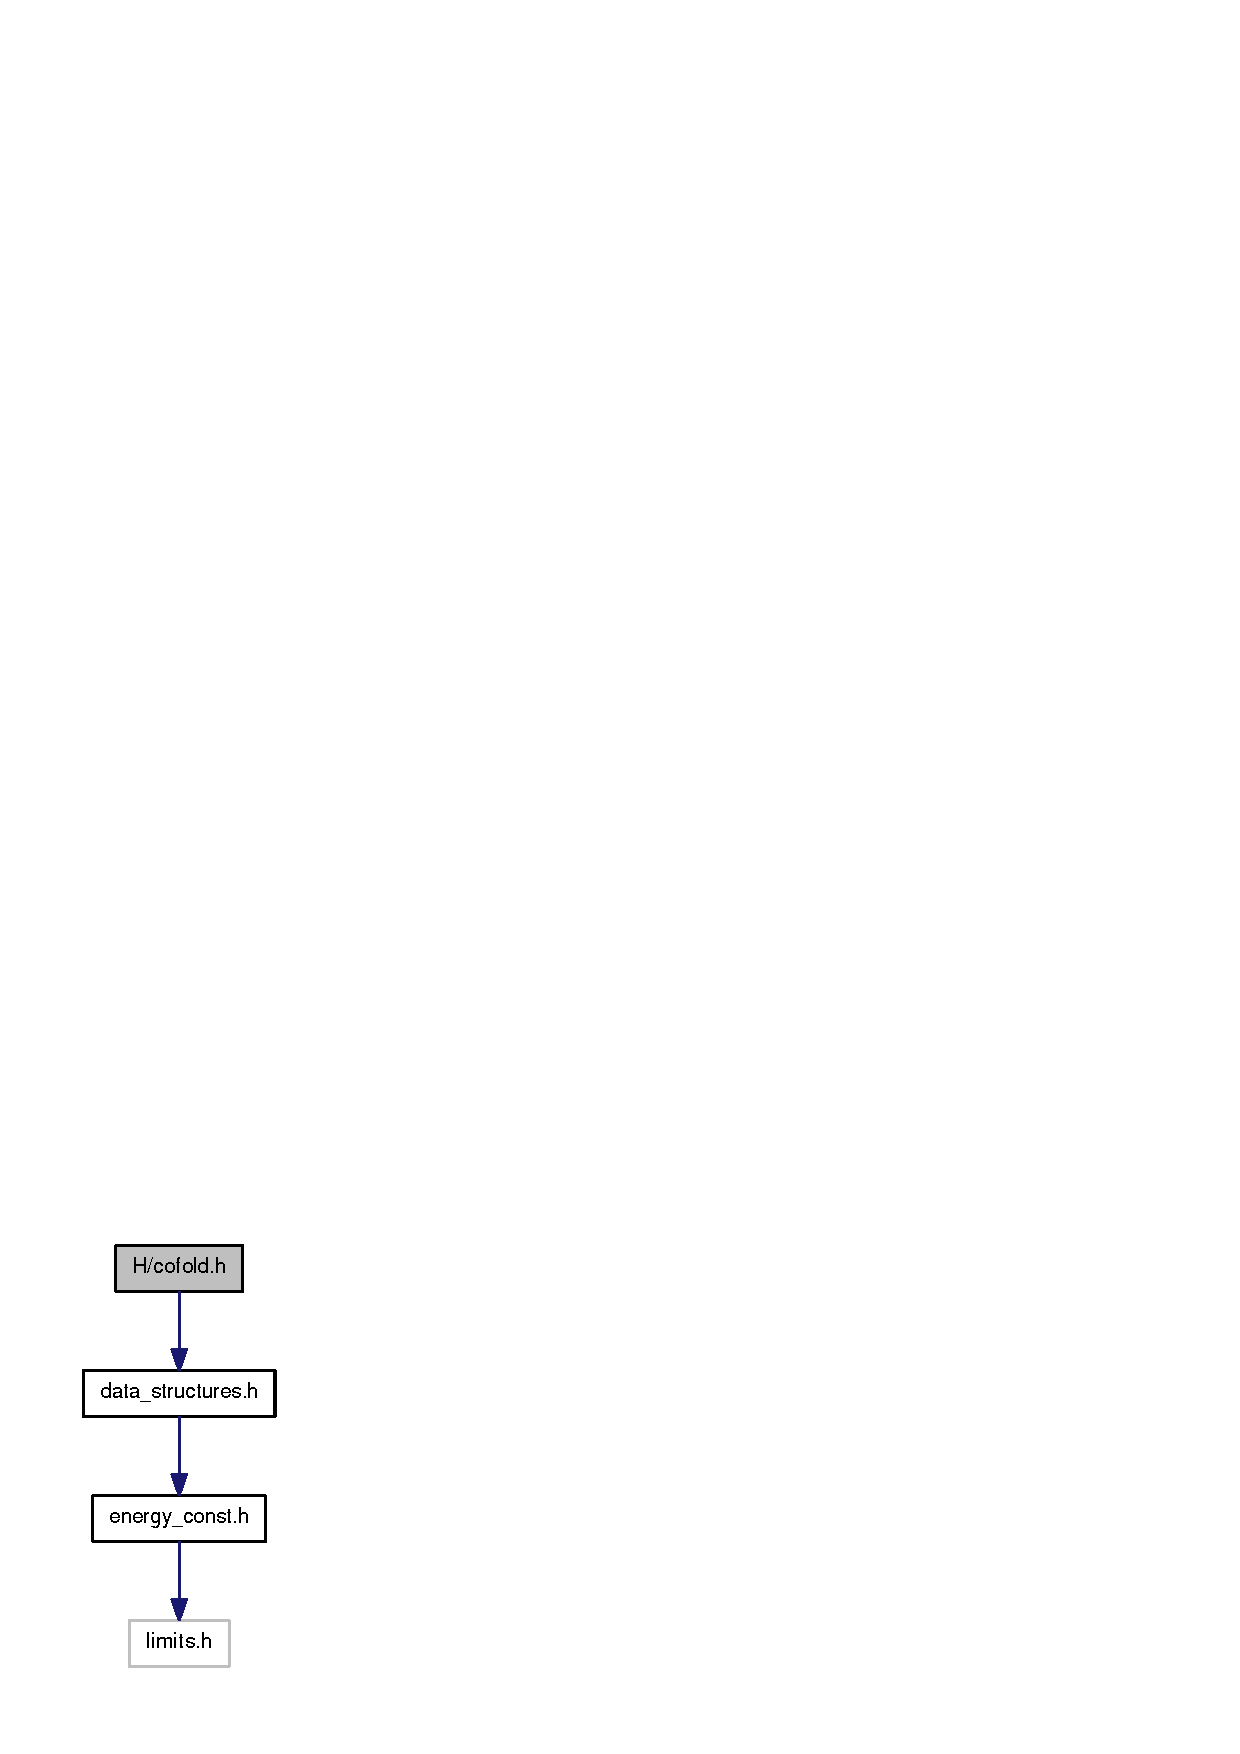
\includegraphics[width=68pt]{cofold_8h__incl}
\end{center}
\end{figure}
\subsection*{Functions}
\begin{DoxyCompactItemize}
\item 
float \hyperlink{cofold_8h_abc8517f22cfe70595ee81fc837910d52}{cofold} (const char $\ast$sequence, char $\ast$structure)
\begin{DoxyCompactList}\small\item\em Compute the minimum free energy of two interacting RNA molecules. \item\end{DoxyCompactList}\item 
\hypertarget{cofold_8h_aafb33d7473eb9af9d1b168ca8761c41a}{
void \hyperlink{cofold_8h_aafb33d7473eb9af9d1b168ca8761c41a}{free\_\-co\_\-arrays} (void)}
\label{cofold_8h_aafb33d7473eb9af9d1b168ca8761c41a}

\begin{DoxyCompactList}\small\item\em Free memory occupied by \hyperlink{cofold_8h_abc8517f22cfe70595ee81fc837910d52}{cofold()}. \item\end{DoxyCompactList}\item 
\hypertarget{cofold_8h_a4fcbf34e77b99bfbb2333d2ab0c41a57}{
void \hyperlink{cofold_8h_a4fcbf34e77b99bfbb2333d2ab0c41a57}{update\_\-cofold\_\-params} (void)}
\label{cofold_8h_a4fcbf34e77b99bfbb2333d2ab0c41a57}

\begin{DoxyCompactList}\small\item\em Recalculate parameters. \item\end{DoxyCompactList}\item 
\hyperlink{structSOLUTION}{SOLUTION} $\ast$ \hyperlink{cofold_8h_a0d5104e3ecf119d8eabd40aa5fe47f90}{zukersubopt} (const char $\ast$string)
\begin{DoxyCompactList}\small\item\em Compute Zuker type suboptimal structures. \item\end{DoxyCompactList}\item 
void \hyperlink{cofold_8h_a4958b517c613e4d2afd5bce6c1060a79}{get\_\-monomere\_\-mfes} (float $\ast$e1, float $\ast$e2)
\begin{DoxyCompactList}\small\item\em get\_\-monomer\_\-free\_\-energies \item\end{DoxyCompactList}\item 
void \hyperlink{cofold_8h_a5cb6b59983f1f74ccc00b9b9c4e84482}{export\_\-cofold\_\-arrays} (int $\ast$$\ast$f5\_\-p, int $\ast$$\ast$c\_\-p, int $\ast$$\ast$fML\_\-p, int $\ast$$\ast$fM1\_\-p, int $\ast$$\ast$fc\_\-p, int $\ast$$\ast$indx\_\-p, char $\ast$$\ast$ptype\_\-p)
\begin{DoxyCompactList}\small\item\em Export the arrays of partition function cofold. \item\end{DoxyCompactList}\item 
void \hyperlink{cofold_8h_afee0c32208aa2ac97338b6e3fbad7fa5}{initialize\_\-cofold} (int length)
\begin{DoxyCompactList}\small\item\em allocate arrays for folding \item\end{DoxyCompactList}\end{DoxyCompactItemize}


\subsection{Detailed Description}
MFE version of cofolding routines. This file includes (almost) all function declarations within the {\bfseries RNAlib} that are related to MFE Cofolding... This also includes the Zuker suboptimals calculations, since they are implemented using the cofold routines. 

\subsection{Function Documentation}
\hypertarget{cofold_8h_abc8517f22cfe70595ee81fc837910d52}{
\index{cofold.h@{cofold.h}!cofold@{cofold}}
\index{cofold@{cofold}!cofold.h@{cofold.h}}
\subsubsection[{cofold}]{\setlength{\rightskip}{0pt plus 5cm}float cofold (const char $\ast$ {\em sequence}, \/  char $\ast$ {\em structure})}}
\label{cofold_8h_abc8517f22cfe70595ee81fc837910d52}


Compute the minimum free energy of two interacting RNA molecules. 

The code is analog to the \hyperlink{fold_8h_aadafcb0f140795ae62e5ca027e335a9b}{fold()} function. If \hyperlink{fold__vars_8h_ab9b2c3a37a5516614c06d0ab54b97cda}{cut\_\-point} ==-\/1 results should be the same as with \hyperlink{fold_8h_aadafcb0f140795ae62e5ca027e335a9b}{fold()}.


\begin{DoxyParams}{Parameters}
\item[{\em sequence}]The two sequences concatenated 
\begin{DoxyParams}{Parameters}
\item[{\em structure}]Will hold the barcket dot structure of the dimer molecule \begin{DoxyReturn}{Returns}
minimum free energy of the structure 
\end{DoxyReturn}
\end{DoxyParams}
\end{DoxyParams}
\hypertarget{cofold_8h_a0d5104e3ecf119d8eabd40aa5fe47f90}{
\index{cofold.h@{cofold.h}!zukersubopt@{zukersubopt}}
\index{zukersubopt@{zukersubopt}!cofold.h@{cofold.h}}
\subsubsection[{zukersubopt}]{\setlength{\rightskip}{0pt plus 5cm}{\bf SOLUTION}$\ast$ zukersubopt (const char $\ast$ {\em string})}}
\label{cofold_8h_a0d5104e3ecf119d8eabd40aa5fe47f90}


Compute Zuker type suboptimal structures. 

Compute Suboptimal structures according to M. Zuker, i.e. for every possible base pair the minimum energy structure containing the resp. base pair. Returns a list of these structures and their energies.


\begin{DoxyParams}{Parameters}
\item[{\em string}]RNA sequence \begin{DoxyReturn}{Returns}
List of zuker suboptimal structures 
\end{DoxyReturn}
\end{DoxyParams}
\hypertarget{cofold_8h_a4958b517c613e4d2afd5bce6c1060a79}{
\index{cofold.h@{cofold.h}!get\_\-monomere\_\-mfes@{get\_\-monomere\_\-mfes}}
\index{get\_\-monomere\_\-mfes@{get\_\-monomere\_\-mfes}!cofold.h@{cofold.h}}
\subsubsection[{get\_\-monomere\_\-mfes}]{\setlength{\rightskip}{0pt plus 5cm}void get\_\-monomere\_\-mfes (float $\ast$ {\em e1}, \/  float $\ast$ {\em e2})}}
\label{cofold_8h_a4958b517c613e4d2afd5bce6c1060a79}


get\_\-monomer\_\-free\_\-energies 

Export monomer free energies out of cofold arrays


\begin{DoxyParams}{Parameters}
\item[{\em e1}]A pointer to a variable where the energy of molecule A will be written to 
\begin{DoxyParams}{Parameters}
\item[{\em e2}]A pointer to a variable where the energy of molecule B will be written to \end{DoxyParams}
\end{DoxyParams}
\hypertarget{cofold_8h_a5cb6b59983f1f74ccc00b9b9c4e84482}{
\index{cofold.h@{cofold.h}!export\_\-cofold\_\-arrays@{export\_\-cofold\_\-arrays}}
\index{export\_\-cofold\_\-arrays@{export\_\-cofold\_\-arrays}!cofold.h@{cofold.h}}
\subsubsection[{export\_\-cofold\_\-arrays}]{\setlength{\rightskip}{0pt plus 5cm}void export\_\-cofold\_\-arrays (int $\ast$$\ast$ {\em f5\_\-p}, \/  int $\ast$$\ast$ {\em c\_\-p}, \/  int $\ast$$\ast$ {\em fML\_\-p}, \/  int $\ast$$\ast$ {\em fM1\_\-p}, \/  int $\ast$$\ast$ {\em fc\_\-p}, \/  int $\ast$$\ast$ {\em indx\_\-p}, \/  char $\ast$$\ast$ {\em ptype\_\-p})}}
\label{cofold_8h_a5cb6b59983f1f74ccc00b9b9c4e84482}


Export the arrays of partition function cofold. 

Export the cofold arrays for use e.g. in the concentration Computations or suboptimal secondary structure backtracking


\begin{DoxyParams}{Parameters}
\item[{\em f5\_\-p}]A pointer to the 'f5' array, i.e. array conatining best free energy in interval \mbox{[}1,j\mbox{]} 
\begin{DoxyParams}{Parameters}
\item[{\em c\_\-p}]A pointer to the 'c' array, i.e. array containing best free energy in interval \mbox{[}i,j\mbox{]} given that i pairs with j 
\begin{DoxyParams}{Parameters}
\item[{\em fML\_\-p}]A pointer to the 'M' array, i.e. array containing best free energy in interval \mbox{[}i,j\mbox{]} for any multiloop segment with at least one stem 
\begin{DoxyParams}{Parameters}
\item[{\em fM1\_\-p}]A pointer to the 'M1' array, i.e. array containing best free energy in interval \mbox{[}i,j\mbox{]} for multiloop segment with exactly one stem 
\begin{DoxyParams}{Parameters}
\item[{\em fc\_\-p}]A pointer to the 'fc' array, i.e. array ... 
\begin{DoxyParams}{Parameters}
\item[{\em indx\_\-p}]A pointer to the indexing array used for accessing the energy matrices 
\begin{DoxyParams}{Parameters}
\item[{\em ptype\_\-p}]A pointer to the ptype array containing the base pair types for each possibility (i,j) \end{DoxyParams}
\end{DoxyParams}
\end{DoxyParams}
\end{DoxyParams}
\end{DoxyParams}
\end{DoxyParams}
\end{DoxyParams}
\hypertarget{cofold_8h_afee0c32208aa2ac97338b6e3fbad7fa5}{
\index{cofold.h@{cofold.h}!initialize\_\-cofold@{initialize\_\-cofold}}
\index{initialize\_\-cofold@{initialize\_\-cofold}!cofold.h@{cofold.h}}
\subsubsection[{initialize\_\-cofold}]{\setlength{\rightskip}{0pt plus 5cm}void initialize\_\-cofold (int {\em length})}}
\label{cofold_8h_afee0c32208aa2ac97338b6e3fbad7fa5}


allocate arrays for folding 

\begin{Desc}
\item[\hyperlink{deprecated__deprecated000001}{Deprecated}]\{This function is obsolete and will be removed soon!\} \end{Desc}

\hypertarget{convert__epars_8h}{
\section{H/convert\_\-epars.h File Reference}
\label{convert__epars_8h}\index{H/convert\_\-epars.h@{H/convert\_\-epars.h}}
}


Functions and definitions for energy parameter file format conversion.  


\subsection*{Defines}
\begin{DoxyCompactItemize}
\item 
\hypertarget{convert__epars_8h_a8dc6aee5a806c49b71557152f9616bc4}{
\#define \hyperlink{convert__epars_8h_a8dc6aee5a806c49b71557152f9616bc4}{VRNA\_\-CONVERT\_\-OUTPUT\_\-ALL}~1U}
\label{convert__epars_8h_a8dc6aee5a806c49b71557152f9616bc4}

\begin{DoxyCompactList}\small\item\em Flag to indicate printing of a complete parameter set. \item\end{DoxyCompactList}\item 
\hypertarget{convert__epars_8h_af66fe2cb11dfcfd32d791049c254a8a4}{
\#define \hyperlink{convert__epars_8h_af66fe2cb11dfcfd32d791049c254a8a4}{VRNA\_\-CONVERT\_\-OUTPUT\_\-HP}~2U}
\label{convert__epars_8h_af66fe2cb11dfcfd32d791049c254a8a4}

\begin{DoxyCompactList}\small\item\em Flag to indicate printing of hairpin contributions. \item\end{DoxyCompactList}\item 
\hypertarget{convert__epars_8h_ad23522d63f8d4c50d5a5deee9bee3ef2}{
\#define \hyperlink{convert__epars_8h_ad23522d63f8d4c50d5a5deee9bee3ef2}{VRNA\_\-CONVERT\_\-OUTPUT\_\-STACK}~4U}
\label{convert__epars_8h_ad23522d63f8d4c50d5a5deee9bee3ef2}

\begin{DoxyCompactList}\small\item\em Flag to indicate printing of base pair stack contributions. \item\end{DoxyCompactList}\item 
\hypertarget{convert__epars_8h_aa892c7b4957459090f3e08da298cc347}{
\#define \hyperlink{convert__epars_8h_aa892c7b4957459090f3e08da298cc347}{VRNA\_\-CONVERT\_\-OUTPUT\_\-MM\_\-HP}~8U}
\label{convert__epars_8h_aa892c7b4957459090f3e08da298cc347}

\begin{DoxyCompactList}\small\item\em Flag to indicate printing of hairpin mismatch contribution. \item\end{DoxyCompactList}\item 
\hypertarget{convert__epars_8h_a4ff223fb1f9c62cd92d9ab811ad03d55}{
\#define \hyperlink{convert__epars_8h_a4ff223fb1f9c62cd92d9ab811ad03d55}{VRNA\_\-CONVERT\_\-OUTPUT\_\-MM\_\-INT}~16U}
\label{convert__epars_8h_a4ff223fb1f9c62cd92d9ab811ad03d55}

\begin{DoxyCompactList}\small\item\em Flag to indicate printing of interior loop mismatch contribution. \item\end{DoxyCompactList}\item 
\hypertarget{convert__epars_8h_af5d3743219f83c6348155cd81e755bbb}{
\#define \hyperlink{convert__epars_8h_af5d3743219f83c6348155cd81e755bbb}{VRNA\_\-CONVERT\_\-OUTPUT\_\-MM\_\-INT\_\-1N}~32U}
\label{convert__epars_8h_af5d3743219f83c6348155cd81e755bbb}

\begin{DoxyCompactList}\small\item\em Flag to indicate printing of 1:n interior loop mismatch contribution. \item\end{DoxyCompactList}\item 
\hypertarget{convert__epars_8h_a78382ec622ba99e0ac2262317bdd7316}{
\#define \hyperlink{convert__epars_8h_a78382ec622ba99e0ac2262317bdd7316}{VRNA\_\-CONVERT\_\-OUTPUT\_\-MM\_\-INT\_\-23}~64U}
\label{convert__epars_8h_a78382ec622ba99e0ac2262317bdd7316}

\begin{DoxyCompactList}\small\item\em Flag to indicate printing of 2:3 interior loop mismatch contribution. \item\end{DoxyCompactList}\item 
\hypertarget{convert__epars_8h_ae67af9f1cdf7baf2865481282a5d1034}{
\#define \hyperlink{convert__epars_8h_ae67af9f1cdf7baf2865481282a5d1034}{VRNA\_\-CONVERT\_\-OUTPUT\_\-MM\_\-MULTI}~128U}
\label{convert__epars_8h_ae67af9f1cdf7baf2865481282a5d1034}

\begin{DoxyCompactList}\small\item\em Flag to indicate printing of multi loop mismatch contribution. \item\end{DoxyCompactList}\item 
\hypertarget{convert__epars_8h_af14ead7ef1fdbe725ade653750fc51e3}{
\#define \hyperlink{convert__epars_8h_af14ead7ef1fdbe725ade653750fc51e3}{VRNA\_\-CONVERT\_\-OUTPUT\_\-MM\_\-EXT}~256U}
\label{convert__epars_8h_af14ead7ef1fdbe725ade653750fc51e3}

\begin{DoxyCompactList}\small\item\em Flag to indicate printing of exterior loop mismatch contribution. \item\end{DoxyCompactList}\item 
\hypertarget{convert__epars_8h_a036ffd996d8c8a9acf631760dd1da24b}{
\#define \hyperlink{convert__epars_8h_a036ffd996d8c8a9acf631760dd1da24b}{VRNA\_\-CONVERT\_\-OUTPUT\_\-DANGLE5}~512U}
\label{convert__epars_8h_a036ffd996d8c8a9acf631760dd1da24b}

\begin{DoxyCompactList}\small\item\em Flag to indicate printing of 5' dangle conctribution. \item\end{DoxyCompactList}\item 
\hypertarget{convert__epars_8h_a34a8a5479ef885834ef32f3fb43d79bc}{
\#define \hyperlink{convert__epars_8h_a34a8a5479ef885834ef32f3fb43d79bc}{VRNA\_\-CONVERT\_\-OUTPUT\_\-DANGLE3}~1024U}
\label{convert__epars_8h_a34a8a5479ef885834ef32f3fb43d79bc}

\begin{DoxyCompactList}\small\item\em Flag to indicate printing of 3' dangle contribution. \item\end{DoxyCompactList}\item 
\hypertarget{convert__epars_8h_a079aafefd5f8ab57ee5120099a34bd25}{
\#define \hyperlink{convert__epars_8h_a079aafefd5f8ab57ee5120099a34bd25}{VRNA\_\-CONVERT\_\-OUTPUT\_\-INT\_\-11}~2048U}
\label{convert__epars_8h_a079aafefd5f8ab57ee5120099a34bd25}

\begin{DoxyCompactList}\small\item\em Flag to indicate printing of 1:1 interior loop contribution. \item\end{DoxyCompactList}\item 
\hypertarget{convert__epars_8h_acf770881d9034431ebe741642342a1f9}{
\#define \hyperlink{convert__epars_8h_acf770881d9034431ebe741642342a1f9}{VRNA\_\-CONVERT\_\-OUTPUT\_\-INT\_\-21}~4096U}
\label{convert__epars_8h_acf770881d9034431ebe741642342a1f9}

\begin{DoxyCompactList}\small\item\em Flag to indicate printing of 2:1 interior loop contribution. \item\end{DoxyCompactList}\item 
\hypertarget{convert__epars_8h_aa307671e2631cdacad9cbe4c6583b05f}{
\#define \hyperlink{convert__epars_8h_aa307671e2631cdacad9cbe4c6583b05f}{VRNA\_\-CONVERT\_\-OUTPUT\_\-INT\_\-22}~8192U}
\label{convert__epars_8h_aa307671e2631cdacad9cbe4c6583b05f}

\begin{DoxyCompactList}\small\item\em Flag to indicate printing of 2:2 interior loop contribution. \item\end{DoxyCompactList}\item 
\hypertarget{convert__epars_8h_a7092fe0be4de6f02cc0bf08e81af726a}{
\#define \hyperlink{convert__epars_8h_a7092fe0be4de6f02cc0bf08e81af726a}{VRNA\_\-CONVERT\_\-OUTPUT\_\-BULGE}~16384U}
\label{convert__epars_8h_a7092fe0be4de6f02cc0bf08e81af726a}

\begin{DoxyCompactList}\small\item\em Flag to indicate printing of bulge loop contribution. \item\end{DoxyCompactList}\item 
\hypertarget{convert__epars_8h_ac5c2289fdf8ff1b980976d1613ff943a}{
\#define \hyperlink{convert__epars_8h_ac5c2289fdf8ff1b980976d1613ff943a}{VRNA\_\-CONVERT\_\-OUTPUT\_\-INT}~32768U}
\label{convert__epars_8h_ac5c2289fdf8ff1b980976d1613ff943a}

\begin{DoxyCompactList}\small\item\em Flag to indicate printing of interior loop contribution. \item\end{DoxyCompactList}\item 
\hypertarget{convert__epars_8h_af2c8755d64eff3852aa45df9ac80a4fe}{
\#define \hyperlink{convert__epars_8h_af2c8755d64eff3852aa45df9ac80a4fe}{VRNA\_\-CONVERT\_\-OUTPUT\_\-ML}~65536U}
\label{convert__epars_8h_af2c8755d64eff3852aa45df9ac80a4fe}

\begin{DoxyCompactList}\small\item\em Flag to indicate printing of multi loop contribution. \item\end{DoxyCompactList}\item 
\hypertarget{convert__epars_8h_a46d5b1535ae86060b6317565b7c6b40b}{
\#define \hyperlink{convert__epars_8h_a46d5b1535ae86060b6317565b7c6b40b}{VRNA\_\-CONVERT\_\-OUTPUT\_\-MISC}~131072U}
\label{convert__epars_8h_a46d5b1535ae86060b6317565b7c6b40b}

\begin{DoxyCompactList}\small\item\em Flag to indicate printing of misc contributions (such as terminalAU). \item\end{DoxyCompactList}\item 
\hypertarget{convert__epars_8h_aa1ff48a79642d69579d1766561ec6db6}{
\#define \hyperlink{convert__epars_8h_aa1ff48a79642d69579d1766561ec6db6}{VRNA\_\-CONVERT\_\-OUTPUT\_\-SPECIAL\_\-HP}~262144U}
\label{convert__epars_8h_aa1ff48a79642d69579d1766561ec6db6}

\begin{DoxyCompactList}\small\item\em Flag to indicate printing of special hairpin contributions (tri-\/, tetra-\/, hexa-\/loops). \item\end{DoxyCompactList}\item 
\hypertarget{convert__epars_8h_a0d4e8a836bb4864ab5129c085dbf592d}{
\#define \hyperlink{convert__epars_8h_a0d4e8a836bb4864ab5129c085dbf592d}{VRNA\_\-CONVERT\_\-OUTPUT\_\-VANILLA}~524288U}
\label{convert__epars_8h_a0d4e8a836bb4864ab5129c085dbf592d}

\begin{DoxyCompactList}\small\item\em Flag to indicate printing of given parameters only\par
\begin{DoxyNote}{Note}
This option overrides all other output options, except \hyperlink{convert__epars_8h_ac86976e9c2a55b3a6481ea60044f6098}{VRNA\_\-CONVERT\_\-OUTPUT\_\-DUMP} ! 
\end{DoxyNote}
\item\end{DoxyCompactList}\item 
\hypertarget{convert__epars_8h_a2eb0462f16939ddacdaf751a88d675ce}{
\#define \hyperlink{convert__epars_8h_a2eb0462f16939ddacdaf751a88d675ce}{VRNA\_\-CONVERT\_\-OUTPUT\_\-NINIO}~1048576U}
\label{convert__epars_8h_a2eb0462f16939ddacdaf751a88d675ce}

\begin{DoxyCompactList}\small\item\em Flag to indicate printing of interior loop asymmetry contribution. \item\end{DoxyCompactList}\item 
\hypertarget{convert__epars_8h_ac86976e9c2a55b3a6481ea60044f6098}{
\#define \hyperlink{convert__epars_8h_ac86976e9c2a55b3a6481ea60044f6098}{VRNA\_\-CONVERT\_\-OUTPUT\_\-DUMP}~2097152U}
\label{convert__epars_8h_ac86976e9c2a55b3a6481ea60044f6098}

\begin{DoxyCompactList}\small\item\em Flag to indicate dumping the energy contributions from the library instead of an input file. \item\end{DoxyCompactList}\end{DoxyCompactItemize}
\subsection*{Functions}
\begin{DoxyCompactItemize}
\item 
void \hyperlink{convert__epars_8h_afbe538bc4eb2cf2a33326e1010005f8a}{convert\_\-parameter\_\-file} (const char $\ast$iname, const char $\ast$oname, unsigned int options)
\begin{DoxyCompactList}\small\item\em Convert/dump a Vienna 1.8.4 formatted energy parameter file. \item\end{DoxyCompactList}\end{DoxyCompactItemize}


\subsection{Detailed Description}
Functions and definitions for energy parameter file format conversion. 

\subsection{Function Documentation}
\hypertarget{convert__epars_8h_afbe538bc4eb2cf2a33326e1010005f8a}{
\index{convert\_\-epars.h@{convert\_\-epars.h}!convert\_\-parameter\_\-file@{convert\_\-parameter\_\-file}}
\index{convert\_\-parameter\_\-file@{convert\_\-parameter\_\-file}!convert_epars.h@{convert\_\-epars.h}}
\subsubsection[{convert\_\-parameter\_\-file}]{\setlength{\rightskip}{0pt plus 5cm}void convert\_\-parameter\_\-file (const char $\ast$ {\em iname}, \/  const char $\ast$ {\em oname}, \/  unsigned int {\em options})}}
\label{convert__epars_8h_afbe538bc4eb2cf2a33326e1010005f8a}


Convert/dump a Vienna 1.8.4 formatted energy parameter file. 

The options argument allows to control the different output modes.\par
 Currently available options are:\par
 \hyperlink{convert__epars_8h_a8dc6aee5a806c49b71557152f9616bc4}{VRNA\_\-CONVERT\_\-OUTPUT\_\-ALL}, \hyperlink{convert__epars_8h_af66fe2cb11dfcfd32d791049c254a8a4}{VRNA\_\-CONVERT\_\-OUTPUT\_\-HP}, \hyperlink{convert__epars_8h_ad23522d63f8d4c50d5a5deee9bee3ef2}{VRNA\_\-CONVERT\_\-OUTPUT\_\-STACK}\par
 \hyperlink{convert__epars_8h_aa892c7b4957459090f3e08da298cc347}{VRNA\_\-CONVERT\_\-OUTPUT\_\-MM\_\-HP}, \hyperlink{convert__epars_8h_a4ff223fb1f9c62cd92d9ab811ad03d55}{VRNA\_\-CONVERT\_\-OUTPUT\_\-MM\_\-INT}, \hyperlink{convert__epars_8h_af5d3743219f83c6348155cd81e755bbb}{VRNA\_\-CONVERT\_\-OUTPUT\_\-MM\_\-INT\_\-1N}\par
 \hyperlink{convert__epars_8h_a78382ec622ba99e0ac2262317bdd7316}{VRNA\_\-CONVERT\_\-OUTPUT\_\-MM\_\-INT\_\-23}, \hyperlink{convert__epars_8h_ae67af9f1cdf7baf2865481282a5d1034}{VRNA\_\-CONVERT\_\-OUTPUT\_\-MM\_\-MULTI}, \hyperlink{convert__epars_8h_af14ead7ef1fdbe725ade653750fc51e3}{VRNA\_\-CONVERT\_\-OUTPUT\_\-MM\_\-EXT}\par
 \hyperlink{convert__epars_8h_a036ffd996d8c8a9acf631760dd1da24b}{VRNA\_\-CONVERT\_\-OUTPUT\_\-DANGLE5}, \hyperlink{convert__epars_8h_a34a8a5479ef885834ef32f3fb43d79bc}{VRNA\_\-CONVERT\_\-OUTPUT\_\-DANGLE3}, \hyperlink{convert__epars_8h_a079aafefd5f8ab57ee5120099a34bd25}{VRNA\_\-CONVERT\_\-OUTPUT\_\-INT\_\-11}\par
 \hyperlink{convert__epars_8h_acf770881d9034431ebe741642342a1f9}{VRNA\_\-CONVERT\_\-OUTPUT\_\-INT\_\-21}, \hyperlink{convert__epars_8h_aa307671e2631cdacad9cbe4c6583b05f}{VRNA\_\-CONVERT\_\-OUTPUT\_\-INT\_\-22}, \hyperlink{convert__epars_8h_a7092fe0be4de6f02cc0bf08e81af726a}{VRNA\_\-CONVERT\_\-OUTPUT\_\-BULGE}\par
 \hyperlink{convert__epars_8h_ac5c2289fdf8ff1b980976d1613ff943a}{VRNA\_\-CONVERT\_\-OUTPUT\_\-INT}, \hyperlink{convert__epars_8h_af2c8755d64eff3852aa45df9ac80a4fe}{VRNA\_\-CONVERT\_\-OUTPUT\_\-ML}, \hyperlink{convert__epars_8h_a46d5b1535ae86060b6317565b7c6b40b}{VRNA\_\-CONVERT\_\-OUTPUT\_\-MISC}\par
 \hyperlink{convert__epars_8h_aa1ff48a79642d69579d1766561ec6db6}{VRNA\_\-CONVERT\_\-OUTPUT\_\-SPECIAL\_\-HP}, \hyperlink{convert__epars_8h_a0d4e8a836bb4864ab5129c085dbf592d}{VRNA\_\-CONVERT\_\-OUTPUT\_\-VANILLA}, \hyperlink{convert__epars_8h_a2eb0462f16939ddacdaf751a88d675ce}{VRNA\_\-CONVERT\_\-OUTPUT\_\-NINIO}\par
 \hyperlink{convert__epars_8h_ac86976e9c2a55b3a6481ea60044f6098}{VRNA\_\-CONVERT\_\-OUTPUT\_\-DUMP}

The defined options are fine for bitwise compare-\/ and assignment-\/operations, e. g.: pass a collection of options as a single value like this: \begin{DoxyVerb}convert_parameter_file(ifile, ofile, option_1 | option_2 | option_n) \end{DoxyVerb}



\begin{DoxyParams}{Parameters}
\item[{\em iname}]The input file name (If NULL input is read from stdin) 
\begin{DoxyParams}{Parameters}
\item[{\em oname}]The output file name (If NULL output is written to stdout) 
\begin{DoxyParams}{Parameters}
\item[{\em options}]The options (as described above) \end{DoxyParams}
\end{DoxyParams}
\end{DoxyParams}

\hypertarget{data__structures_8h}{
\section{H/data\_\-structures.h File Reference}
\label{data__structures_8h}\index{H/data\_\-structures.h@{H/data\_\-structures.h}}
}


All datastructures and typedefs shared among the Vienna RNA Package can be found here.  


Include dependency graph for data\_\-structures.h:\nopagebreak
\begin{figure}[H]
\begin{center}
\leavevmode
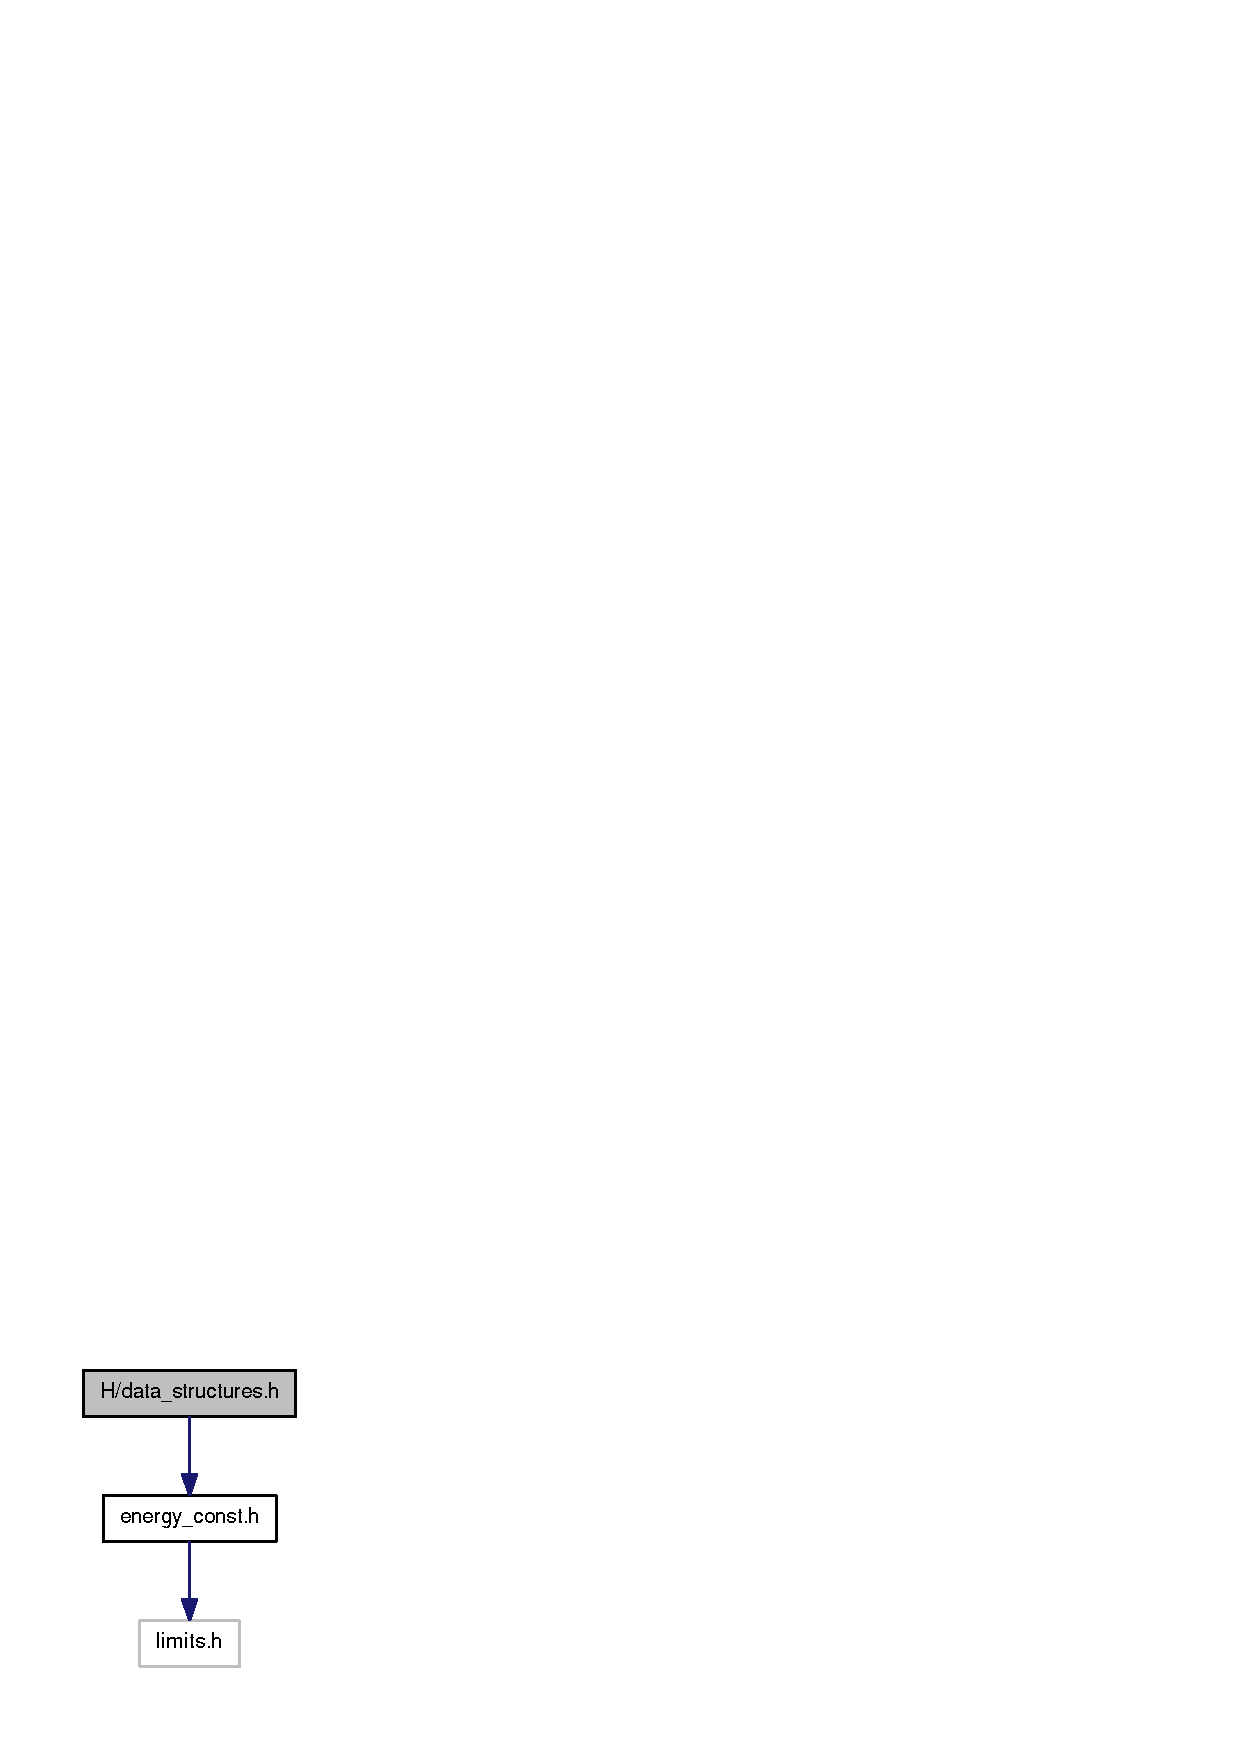
\includegraphics[width=73pt]{data__structures_8h__incl}
\end{center}
\end{figure}
This graph shows which files directly or indirectly include this file:\nopagebreak
\begin{figure}[H]
\begin{center}
\leavevmode
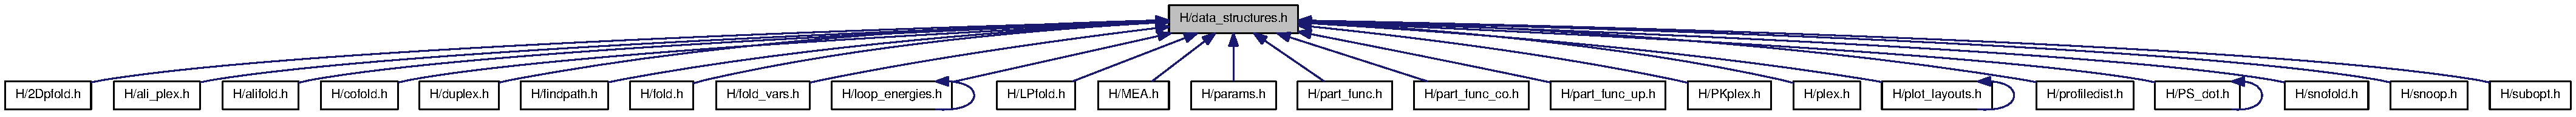
\includegraphics[width=420pt]{data__structures_8h__dep__incl}
\end{center}
\end{figure}
\subsection*{Data Structures}
\begin{DoxyCompactItemize}
\item 
struct \hyperlink{structplist}{plist}
\begin{DoxyCompactList}\small\item\em this datastructure is used as input parameter in functions of \hyperlink{PS__dot_8h}{PS\_\-dot.h} and others \item\end{DoxyCompactList}\item 
struct \hyperlink{structcpair}{cpair}
\begin{DoxyCompactList}\small\item\em this datastructure is used as input parameter in functions of PS\_\-dot.c \item\end{DoxyCompactList}\item 
struct \hyperlink{structCOORDINATE}{COORDINATE}
\begin{DoxyCompactList}\small\item\em this is a workarround for the SWIG Perl Wrapper RNA plot function that returns an array of type \hyperlink{structCOORDINATE}{COORDINATE} \item\end{DoxyCompactList}\item 
struct \hyperlink{structsect}{sect}
\begin{DoxyCompactList}\small\item\em stack of partial structures for backtracking \item\end{DoxyCompactList}\item 
struct \hyperlink{structbondT}{bondT}
\begin{DoxyCompactList}\small\item\em base pair \item\end{DoxyCompactList}\item 
struct \hyperlink{structbondTEn}{bondTEn}
\begin{DoxyCompactList}\small\item\em base pair with associated energy \item\end{DoxyCompactList}\item 
struct \hyperlink{structmodel__detailsT}{model\_\-detailsT}
\begin{DoxyCompactList}\small\item\em The data structure that contains the complete model details used throughout the calculations. \item\end{DoxyCompactList}\item 
struct \hyperlink{structparamT}{paramT}
\begin{DoxyCompactList}\small\item\em The datastructure that contains temperature scaled energy parameters. \item\end{DoxyCompactList}\item 
struct \hyperlink{structpf__paramT}{pf\_\-paramT}
\begin{DoxyCompactList}\small\item\em The datastructure that contains temperature scaled Boltzmann weights of the energy parameters. \item\end{DoxyCompactList}\item 
struct \hyperlink{structPAIR}{PAIR}
\begin{DoxyCompactList}\small\item\em base pair data structure used in subopt.c \item\end{DoxyCompactList}\item 
struct \hyperlink{structINTERVAL}{INTERVAL}
\begin{DoxyCompactList}\small\item\em sequence interval stack element used in subopt.c \item\end{DoxyCompactList}\item 
struct \hyperlink{structSOLUTION}{SOLUTION}
\begin{DoxyCompactList}\small\item\em solution element from subopt.c \item\end{DoxyCompactList}\item 
struct \hyperlink{structcofoldF}{cofoldF}
\item 
struct \hyperlink{structConcEnt}{ConcEnt}
\item 
struct \hyperlink{structpairpro}{pairpro}
\item 
struct \hyperlink{structpair__info}{pair\_\-info}
\begin{DoxyCompactList}\small\item\em A base pair info structure. \item\end{DoxyCompactList}\item 
struct \hyperlink{structmove__t}{move\_\-t}
\item 
struct \hyperlink{structintermediate__t}{intermediate\_\-t}
\item 
struct \hyperlink{structpath__t}{path\_\-t}
\item 
struct \hyperlink{structpu__contrib}{pu\_\-contrib}
\item 
struct \hyperlink{structinteract}{interact}
\item 
struct \hyperlink{structpu__out}{pu\_\-out}
\item 
struct \hyperlink{structconstrain}{constrain}
\item 
struct \hyperlink{structduplexT}{duplexT}
\item 
struct \hyperlink{structfolden}{folden}
\item 
struct \hyperlink{structsnoopT}{snoopT}
\item 
struct \hyperlink{structdupVar}{dupVar}
\item 
struct \hyperlink{structTwoDfold__solution}{TwoDfold\_\-solution}
\begin{DoxyCompactList}\small\item\em Solution element returned from TwoDfoldList. \item\end{DoxyCompactList}\item 
struct \hyperlink{structTwoDfold__vars}{TwoDfold\_\-vars}
\begin{DoxyCompactList}\small\item\em Variables compound for 2Dfold MFE folding. \item\end{DoxyCompactList}\item 
struct \hyperlink{structTwoDpfold__solution}{TwoDpfold\_\-solution}
\begin{DoxyCompactList}\small\item\em Solution element returned from TwoDpfoldList. \item\end{DoxyCompactList}\item 
struct \hyperlink{structTwoDpfold__vars}{TwoDpfold\_\-vars}
\begin{DoxyCompactList}\small\item\em Variables compound for 2Dfold partition function folding. \item\end{DoxyCompactList}\end{DoxyCompactItemize}
\subsection*{Defines}
\begin{DoxyCompactItemize}
\item 
\hypertarget{data__structures_8h_a05a5ffe718aa431d97419a12fb082379}{
\#define \hyperlink{data__structures_8h_a05a5ffe718aa431d97419a12fb082379}{MAXALPHA}~20}
\label{data__structures_8h_a05a5ffe718aa431d97419a12fb082379}

\begin{DoxyCompactList}\small\item\em Maximal length of alphabet. \item\end{DoxyCompactList}\item 
\hypertarget{data__structures_8h_a5ec740b80afb4906ba4311dbd8ddbd89}{
\#define \hyperlink{data__structures_8h_a5ec740b80afb4906ba4311dbd8ddbd89}{MAXDOS}~1000}
\label{data__structures_8h_a5ec740b80afb4906ba4311dbd8ddbd89}

\begin{DoxyCompactList}\small\item\em Maximum density of states discretization for subopt. \item\end{DoxyCompactList}\end{DoxyCompactItemize}


\subsection{Detailed Description}
All datastructures and typedefs shared among the Vienna RNA Package can be found here. 
\hypertarget{dist__vars_8h}{
\section{H/dist\_\-vars.h File Reference}
\label{dist__vars_8h}\index{H/dist\_\-vars.h@{H/dist\_\-vars.h}}
}


Global variables for Distance-\/Package.  


This graph shows which files directly or indirectly include this file:\nopagebreak
\begin{figure}[H]
\begin{center}
\leavevmode
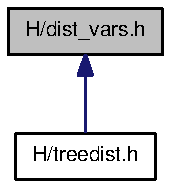
\includegraphics[width=59pt]{dist__vars_8h__dep__incl}
\end{center}
\end{figure}
\subsection*{Data Structures}
\begin{DoxyCompactItemize}
\item 
struct \hyperlink{structPostorder__list}{Postorder\_\-list}
\item 
struct \hyperlink{structTree}{Tree}
\item 
struct \hyperlink{structswString}{swString}
\end{DoxyCompactItemize}
\subsection*{Variables}
\begin{DoxyCompactItemize}
\item 
int \hyperlink{dist__vars_8h_aa03194c513af6b860e7b33e370b82bdb}{edit\_\-backtrack}
\begin{DoxyCompactList}\small\item\em Produce an alignment of the two structures being compared by tracing the editing path giving the minimum distance. \item\end{DoxyCompactList}\item 
\hypertarget{dist__vars_8h_ac1605fe3448ad0a0b809c4fb8f6a854a}{
char $\ast$ \hyperlink{dist__vars_8h_ac1605fe3448ad0a0b809c4fb8f6a854a}{aligned\_\-line} \mbox{[}4\mbox{]}}
\label{dist__vars_8h_ac1605fe3448ad0a0b809c4fb8f6a854a}

\begin{DoxyCompactList}\small\item\em Contains the two aligned structures after a call to one of the distance functions with \hyperlink{dist__vars_8h_aa03194c513af6b860e7b33e370b82bdb}{edit\_\-backtrack} set to 1. \item\end{DoxyCompactList}\item 
int \hyperlink{dist__vars_8h_ab65d8ff14c6937612212526a60f59b3c}{cost\_\-matrix}
\begin{DoxyCompactList}\small\item\em Specify the cost matrix to be used for distance calculations. \item\end{DoxyCompactList}\end{DoxyCompactItemize}


\subsection{Detailed Description}
Global variables for Distance-\/Package. 

\subsection{Variable Documentation}
\hypertarget{dist__vars_8h_aa03194c513af6b860e7b33e370b82bdb}{
\index{dist\_\-vars.h@{dist\_\-vars.h}!edit\_\-backtrack@{edit\_\-backtrack}}
\index{edit\_\-backtrack@{edit\_\-backtrack}!dist_vars.h@{dist\_\-vars.h}}
\subsubsection[{edit\_\-backtrack}]{\setlength{\rightskip}{0pt plus 5cm}int {\bf edit\_\-backtrack}}}
\label{dist__vars_8h_aa03194c513af6b860e7b33e370b82bdb}


Produce an alignment of the two structures being compared by tracing the editing path giving the minimum distance. 

set to 1 if you want backtracking \hypertarget{dist__vars_8h_ab65d8ff14c6937612212526a60f59b3c}{
\index{dist\_\-vars.h@{dist\_\-vars.h}!cost\_\-matrix@{cost\_\-matrix}}
\index{cost\_\-matrix@{cost\_\-matrix}!dist_vars.h@{dist\_\-vars.h}}
\subsubsection[{cost\_\-matrix}]{\setlength{\rightskip}{0pt plus 5cm}int {\bf cost\_\-matrix}}}
\label{dist__vars_8h_ab65d8ff14c6937612212526a60f59b3c}


Specify the cost matrix to be used for distance calculations. 

if 0, use the default cost matrix (upper matrix in example), otherwise use Shapiro's costs (lower matrix). 
\hypertarget{duplex_8h}{
\section{H/duplex.h File Reference}
\label{duplex_8h}\index{H/duplex.h@{H/duplex.h}}
}


Duplex folding function declarations.  


Include dependency graph for duplex.h:\nopagebreak
\begin{figure}[H]
\begin{center}
\leavevmode
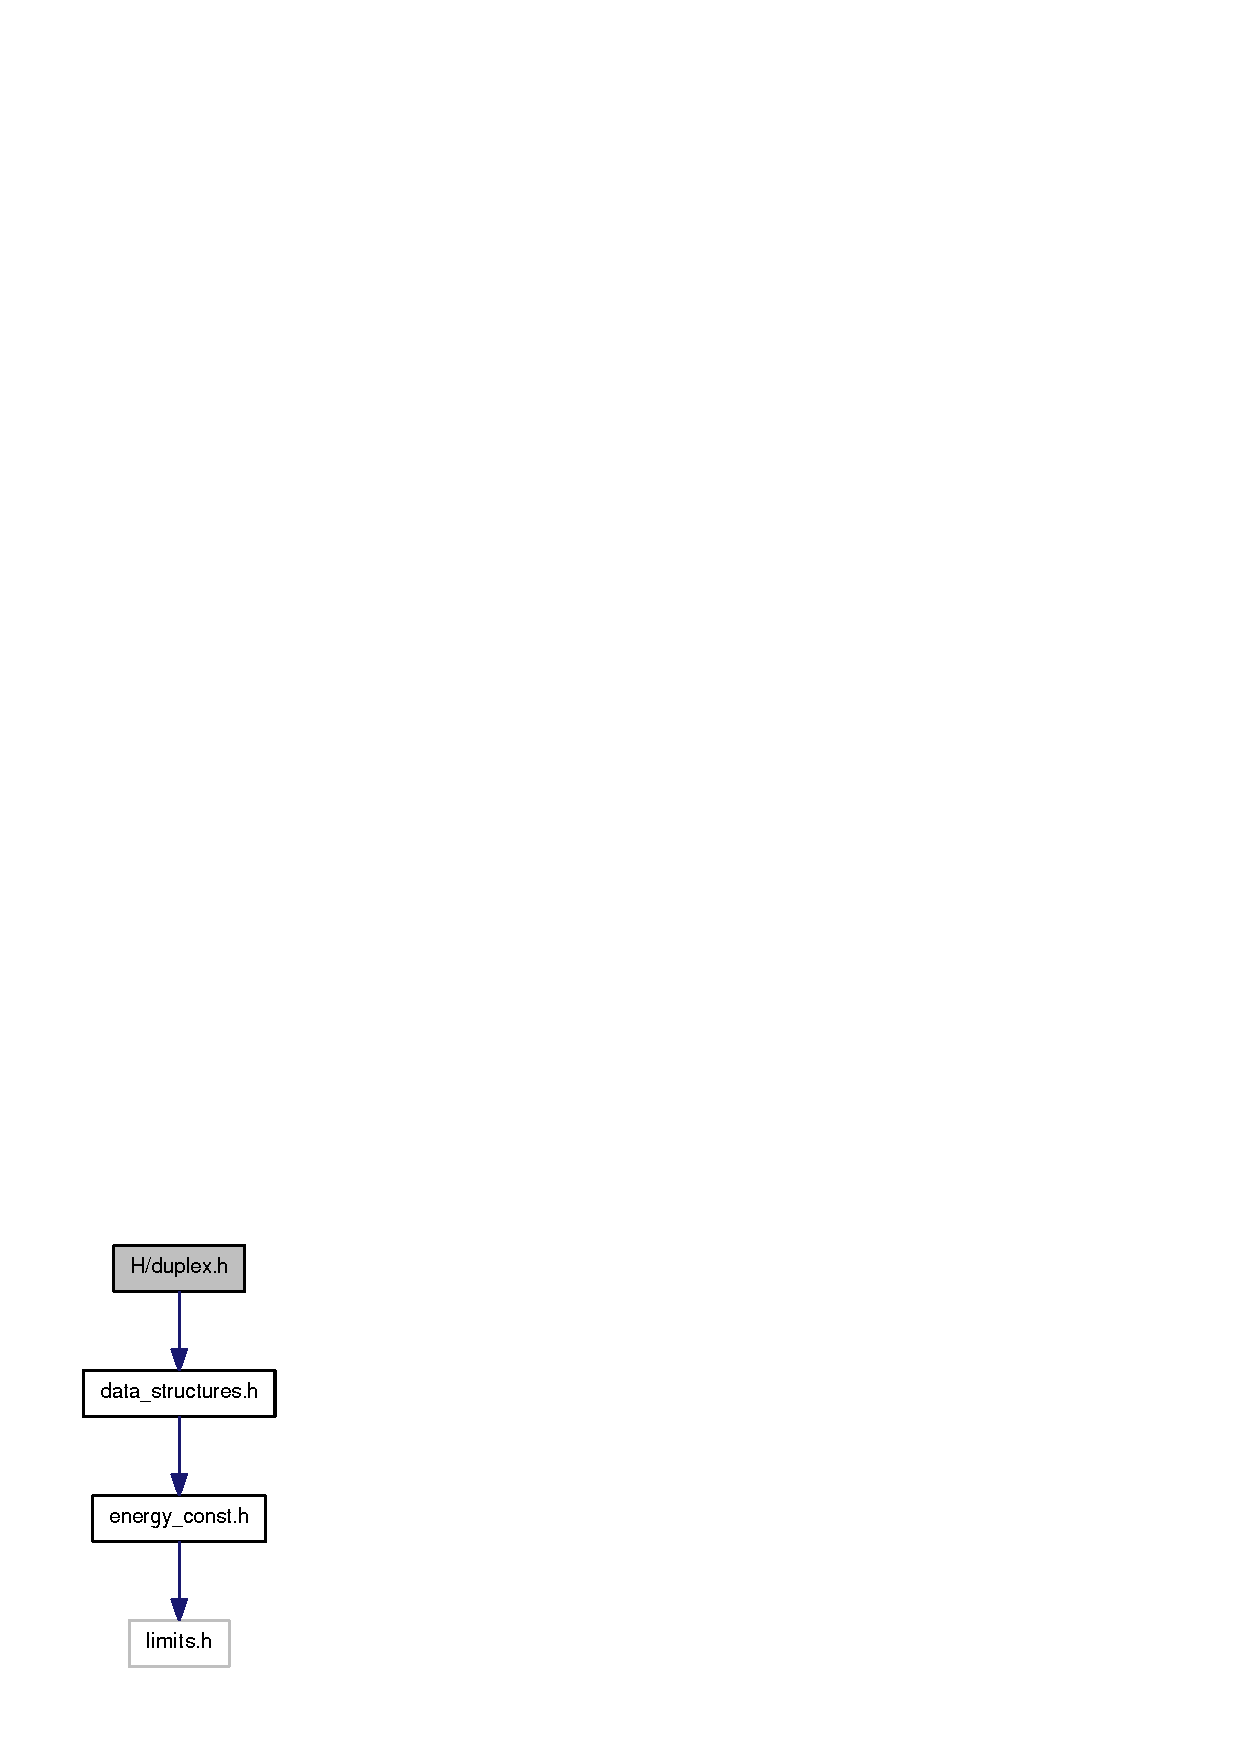
\includegraphics[width=68pt]{duplex_8h__incl}
\end{center}
\end{figure}


\subsection{Detailed Description}
Duplex folding function declarations. .. 
\hypertarget{edit__cost_8h}{
\section{H/edit\_\-cost.h File Reference}
\label{edit__cost_8h}\index{H/edit\_\-cost.h@{H/edit\_\-cost.h}}
}


global variables for Edit Costs included by treedist.c and stringdist.c  




\subsection{Detailed Description}
global variables for Edit Costs included by treedist.c and stringdist.c 
\hypertarget{energy__const_8h}{
\section{H/energy\_\-const.h File Reference}
\label{energy__const_8h}\index{H/energy\_\-const.h@{H/energy\_\-const.h}}
}


energy constants  


Include dependency graph for energy\_\-const.h:\nopagebreak
\begin{figure}[H]
\begin{center}
\leavevmode
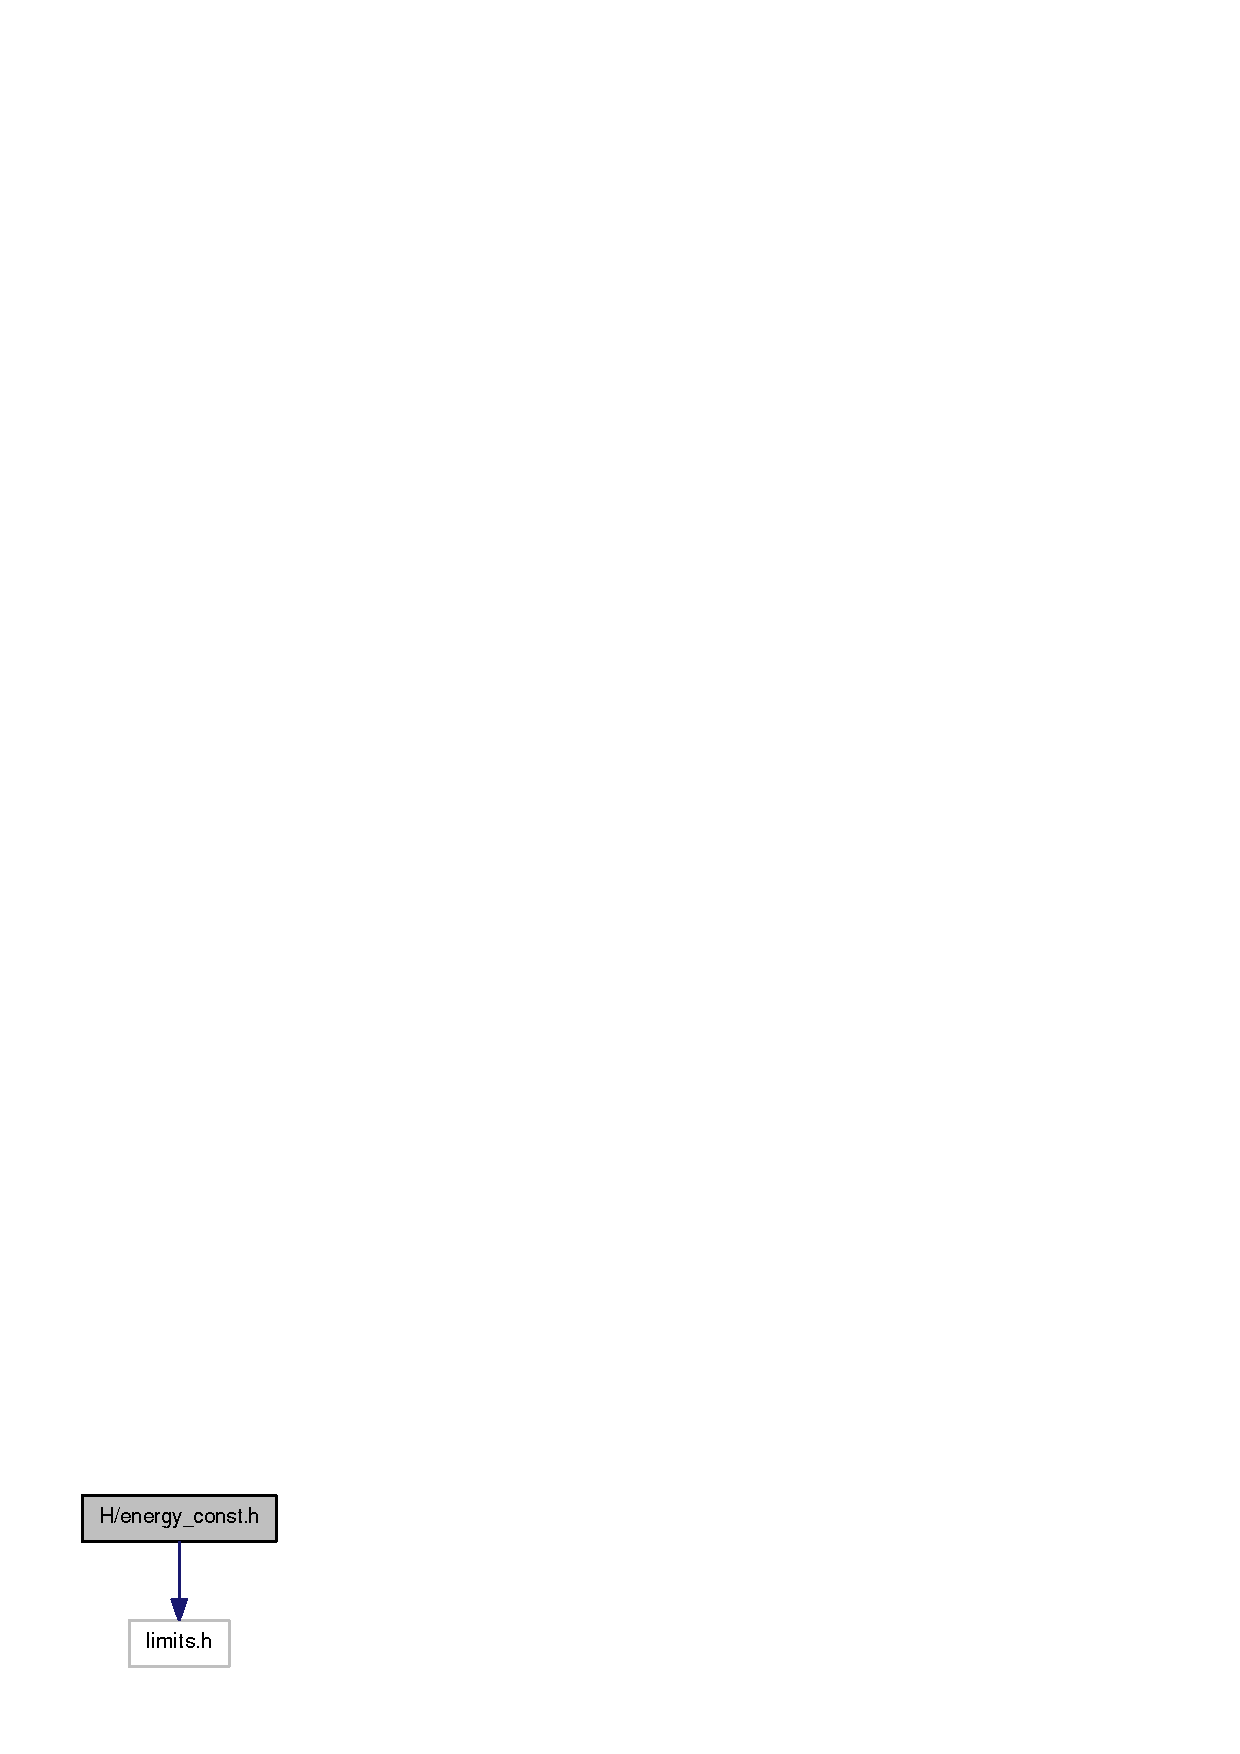
\includegraphics[width=68pt]{energy__const_8h__incl}
\end{center}
\end{figure}
This graph shows which files directly or indirectly include this file:\nopagebreak
\begin{figure}[H]
\begin{center}
\leavevmode
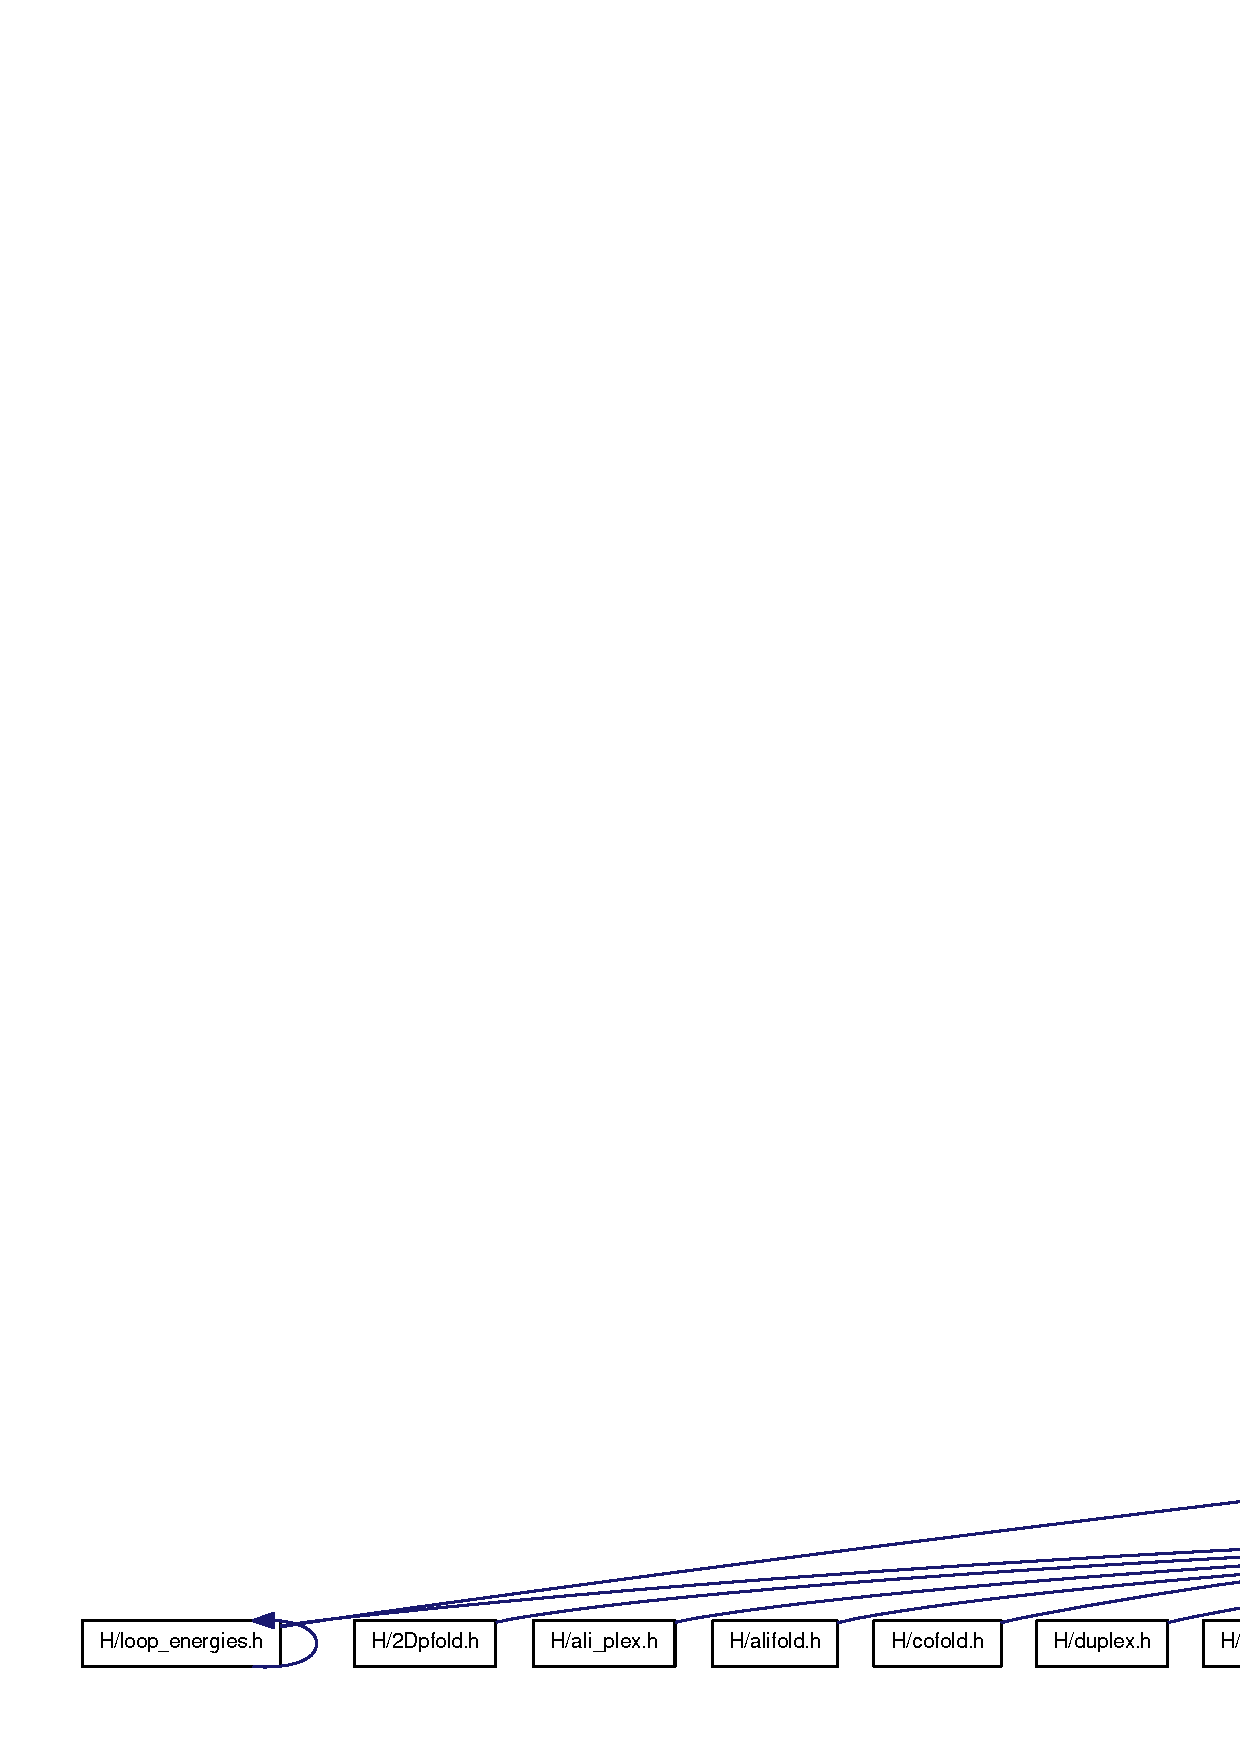
\includegraphics[width=420pt]{energy__const_8h__dep__incl}
\end{center}
\end{figure}
\subsection*{Defines}
\begin{DoxyCompactItemize}
\item 
\hypertarget{energy__const_8h_ab1e4a8d82f24ed5db01dde5f25269cf1}{
\#define \hyperlink{energy__const_8h_ab1e4a8d82f24ed5db01dde5f25269cf1}{GASCONST}~1.98717}
\label{energy__const_8h_ab1e4a8d82f24ed5db01dde5f25269cf1}

\begin{DoxyCompactList}\small\item\em The gas constant. \item\end{DoxyCompactList}\item 
\hypertarget{energy__const_8h_a307c72605e3713972b4f4fb2d53ea20e}{
\#define \hyperlink{energy__const_8h_a307c72605e3713972b4f4fb2d53ea20e}{K0}~273.15}
\label{energy__const_8h_a307c72605e3713972b4f4fb2d53ea20e}

\begin{DoxyCompactList}\small\item\em 0 deg Celsius in Kelvin \item\end{DoxyCompactList}\item 
\hypertarget{energy__const_8h_a12c2040f25d8e3a7b9e1c2024c618cb6}{
\#define \hyperlink{energy__const_8h_a12c2040f25d8e3a7b9e1c2024c618cb6}{INF}~(INT\_\-MAX/10)}
\label{energy__const_8h_a12c2040f25d8e3a7b9e1c2024c618cb6}

\begin{DoxyCompactList}\small\item\em Infinity as used in minimization routines. \item\end{DoxyCompactList}\item 
\hypertarget{energy__const_8h_a5064c29ab2d1e20c2304b3c67562774d}{
\#define \hyperlink{energy__const_8h_a5064c29ab2d1e20c2304b3c67562774d}{FORBIDDEN}~9999}
\label{energy__const_8h_a5064c29ab2d1e20c2304b3c67562774d}

\begin{DoxyCompactList}\small\item\em forbidden \item\end{DoxyCompactList}\item 
\hypertarget{energy__const_8h_a96a9822fa134450197dd454b1478a193}{
\#define \hyperlink{energy__const_8h_a96a9822fa134450197dd454b1478a193}{BONUS}~10000}
\label{energy__const_8h_a96a9822fa134450197dd454b1478a193}

\begin{DoxyCompactList}\small\item\em bonus contribution \item\end{DoxyCompactList}\item 
\hypertarget{energy__const_8h_a5e75221c779d618eab81e096f37e32ce}{
\#define \hyperlink{energy__const_8h_a5e75221c779d618eab81e096f37e32ce}{NBPAIRS}~7}
\label{energy__const_8h_a5e75221c779d618eab81e096f37e32ce}

\begin{DoxyCompactList}\small\item\em The number of distinguishable base pairs. \item\end{DoxyCompactList}\item 
\hypertarget{energy__const_8h_ae646250fd59311356c7e5722a81c3a96}{
\#define \hyperlink{energy__const_8h_ae646250fd59311356c7e5722a81c3a96}{TURN}~3}
\label{energy__const_8h_ae646250fd59311356c7e5722a81c3a96}

\begin{DoxyCompactList}\small\item\em The minimum loop length. \item\end{DoxyCompactList}\item 
\hypertarget{energy__const_8h_ad1bd6eabac419670ddd3c9ed82145988}{
\#define \hyperlink{energy__const_8h_ad1bd6eabac419670ddd3c9ed82145988}{MAXLOOP}~30}
\label{energy__const_8h_ad1bd6eabac419670ddd3c9ed82145988}

\begin{DoxyCompactList}\small\item\em The maximum loop length. \item\end{DoxyCompactList}\end{DoxyCompactItemize}


\subsection{Detailed Description}
energy constants 
\hypertarget{findpath_8h}{
\section{H/findpath.h File Reference}
\label{findpath_8h}\index{H/findpath.h@{H/findpath.h}}
}


Compute direct refolding paths between two secondary structures.  


Include dependency graph for findpath.h:\nopagebreak
\begin{figure}[H]
\begin{center}
\leavevmode
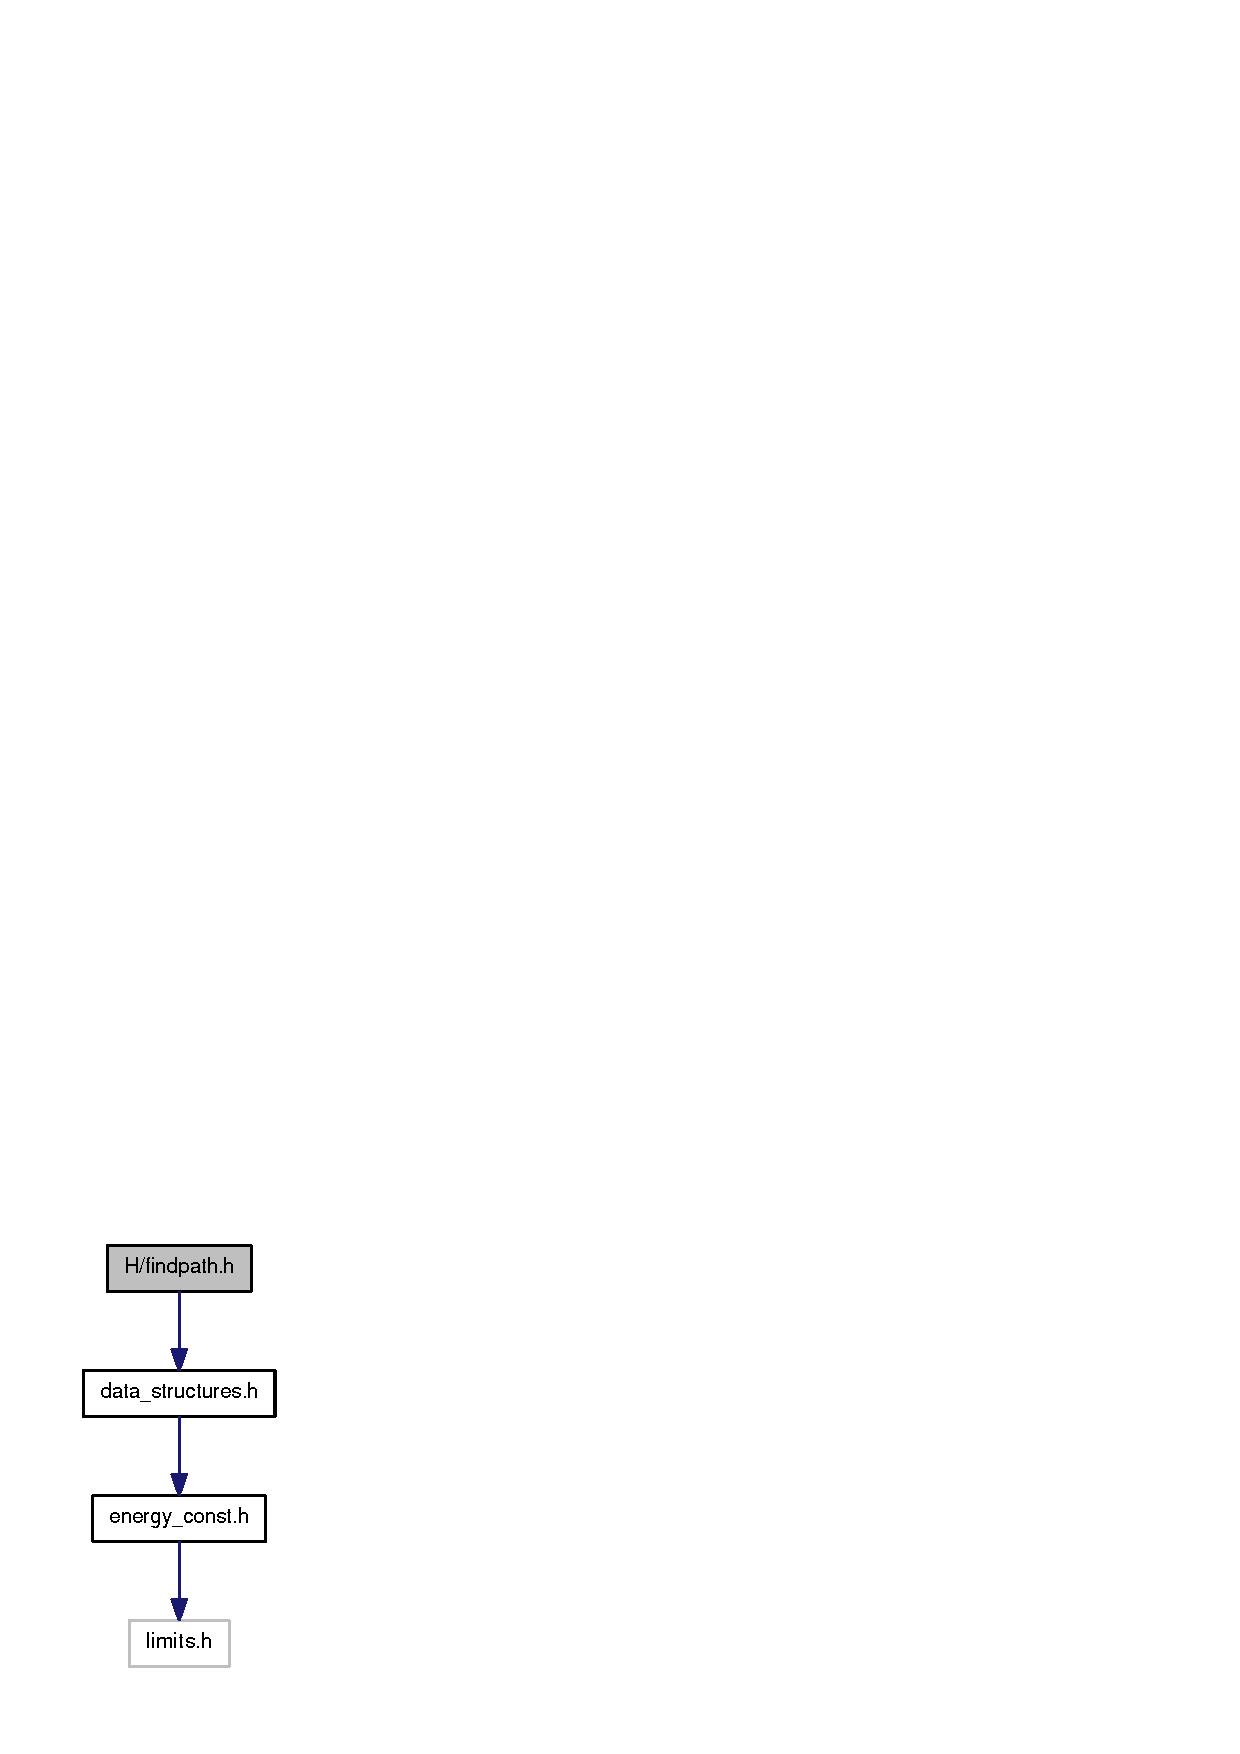
\includegraphics[width=68pt]{findpath_8h__incl}
\end{center}
\end{figure}


\subsection{Detailed Description}
Compute direct refolding paths between two secondary structures. 
\hypertarget{fold_8h}{
\section{H/fold.h File Reference}
\label{fold_8h}\index{H/fold.h@{H/fold.h}}
}


MFE calculations and energy evaluations for single RNA sequences.  


Include dependency graph for fold.h:\nopagebreak
\begin{figure}[H]
\begin{center}
\leavevmode
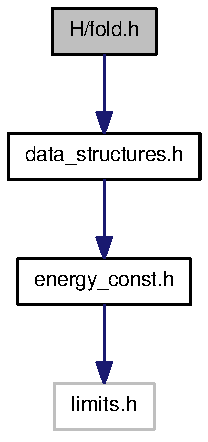
\includegraphics[width=68pt]{fold_8h__incl}
\end{center}
\end{figure}
\subsection*{Functions}
\begin{DoxyCompactItemize}
\item 
float \hyperlink{fold_8h_adb973133c241d57c04b253df35e4d34e}{fold\_\-par} (const char $\ast$sequence, char $\ast$structure, \hyperlink{structparamT}{paramT} $\ast$parameters, int is\_\-constrained, int is\_\-circular)
\begin{DoxyCompactList}\small\item\em Compute minimum free energy and an appropriate secondary structure of an RNA sequence. \item\end{DoxyCompactList}\item 
float \hyperlink{fold_8h_aadafcb0f140795ae62e5ca027e335a9b}{fold} (const char $\ast$sequence, char $\ast$structure)
\begin{DoxyCompactList}\small\item\em Compute minimum free energy and an appropriate secondary structure of an RNA sequence. \item\end{DoxyCompactList}\item 
float \hyperlink{fold_8h_a4ac63ab3e8d9a80ced28b8052d94e423}{circfold} (const char $\ast$sequence, char $\ast$structure)
\begin{DoxyCompactList}\small\item\em Compute minimum free energy and an appropriate secondary structure of a circular RNA sequence. \item\end{DoxyCompactList}\item 
float \hyperlink{fold_8h_af93986cb3cb29770ec9cca69c9fab8cf}{energy\_\-of\_\-structure} (const char $\ast$string, const char $\ast$structure, int verbosity\_\-level)
\begin{DoxyCompactList}\small\item\em Calculate the free energy of an already folded RNA using global model detail settings. \item\end{DoxyCompactList}\item 
float \hyperlink{fold_8h_ab5169ea4f72f250e43811463a33f4e40}{energy\_\-of\_\-struct\_\-par} (const char $\ast$string, const char $\ast$structure, \hyperlink{structparamT}{paramT} $\ast$parameters, int verbosity\_\-level)
\begin{DoxyCompactList}\small\item\em Calculate the free energy of an already folded RNA. \item\end{DoxyCompactList}\item 
float \hyperlink{fold_8h_aeb14f3664aec67fc03268ac75253f0f8}{energy\_\-of\_\-circ\_\-structure} (const char $\ast$string, const char $\ast$structure, int verbosity\_\-level)
\begin{DoxyCompactList}\small\item\em Calculate the free energy of an already folded circular RNA. \item\end{DoxyCompactList}\item 
float \hyperlink{fold_8h_a75dc765ee4a1177832bc817c94cf88e5}{energy\_\-of\_\-circ\_\-struct\_\-par} (const char $\ast$string, const char $\ast$structure, \hyperlink{structparamT}{paramT} $\ast$parameters, int verbosity\_\-level)
\begin{DoxyCompactList}\small\item\em Calculate the free energy of an already folded circular RNA. \item\end{DoxyCompactList}\item 
int \hyperlink{fold_8h_a8831445966b761417e713360791299d8}{energy\_\-of\_\-structure\_\-pt} (const char $\ast$string, short $\ast$ptable, short $\ast$s, short $\ast$s1, int verbosity\_\-level)
\begin{DoxyCompactList}\small\item\em Calculate the free energy of an already folded RNA. \item\end{DoxyCompactList}\item 
int \hyperlink{fold_8h_ada4701dd7519b29da75ceac147601f4e}{energy\_\-of\_\-struct\_\-pt\_\-par} (const char $\ast$string, short $\ast$ptable, short $\ast$s, short $\ast$s1, \hyperlink{structparamT}{paramT} $\ast$parameters, int verbosity\_\-level)
\begin{DoxyCompactList}\small\item\em Calculate the free energy of an already folded RNA. \item\end{DoxyCompactList}\item 
\hypertarget{fold_8h_a107fdfe5fd641868156bfd849f6866c7}{
void \hyperlink{fold_8h_a107fdfe5fd641868156bfd849f6866c7}{free\_\-arrays} (void)}
\label{fold_8h_a107fdfe5fd641868156bfd849f6866c7}

\begin{DoxyCompactList}\small\item\em Free arrays for mfe folding. \item\end{DoxyCompactList}\item 
void \hyperlink{fold_8h_a87b7869bd1d8dc79c60775c74e009e9b}{parenthesis\_\-structure} (char $\ast$structure, \hyperlink{structbondT}{bondT} $\ast$bp, int length)
\begin{DoxyCompactList}\small\item\em Create a dot-\/backet/parenthesis structure from backtracking stack. \item\end{DoxyCompactList}\item 
void \hyperlink{fold_8h_a325f3835c68f34fe833b2b7a5828857f}{parenthesis\_\-zuker} (char $\ast$structure, \hyperlink{structbondT}{bondT} $\ast$bp, int length)
\begin{DoxyCompactList}\small\item\em Create a dot-\/backet/parenthesis structure from backtracking stack obtained by zuker suboptimal calculation in cofold.c. \item\end{DoxyCompactList}\item 
\hypertarget{fold_8h_a41bf8f6fa15b94471f7095cad9f0ccf3}{
void \hyperlink{fold_8h_a41bf8f6fa15b94471f7095cad9f0ccf3}{update\_\-fold\_\-params} (void)}
\label{fold_8h_a41bf8f6fa15b94471f7095cad9f0ccf3}

\begin{DoxyCompactList}\small\item\em Recalculate energy parameters. \item\end{DoxyCompactList}\item 
void \hyperlink{fold_8h_adaa59b81664e2e36cb9932e891558fae}{assign\_\-plist\_\-from\_\-db} (\hyperlink{structplist}{plist} $\ast$$\ast$pl, const char $\ast$struc, float \hyperlink{fold__vars_8h_ac98ec419070aee6831b44e5c700f090f}{pr})
\begin{DoxyCompactList}\small\item\em Create a plist from a dot-\/bracket string. \item\end{DoxyCompactList}\item 
int \hyperlink{fold_8h_a2163034a25c6115d894b199e97e03f6c}{LoopEnergy} (int n1, int n2, int type, int type\_\-2, int si1, int sj1, int sp1, int sq1)
\item 
int \hyperlink{fold_8h_ab327ce11972f5ac069d52c8dedfdb700}{HairpinE} (int size, int type, int si1, int sj1, const char $\ast$string)
\item 
void \hyperlink{fold_8h_ac3f0a28d9cb609d388b155445073fd20}{initialize\_\-fold} (int length)
\begin{DoxyCompactList}\small\item\em Allocate arrays for folding\par
. \item\end{DoxyCompactList}\item 
float \hyperlink{fold_8h_ac2b37fea2145c94d925a3f33378ef87b}{energy\_\-of\_\-struct} (const char $\ast$string, const char $\ast$structure)
\begin{DoxyCompactList}\small\item\em Calculate the free energy of an already folded RNA. \item\end{DoxyCompactList}\item 
int \hyperlink{fold_8h_a27ce6f68512d43bf1fe14a06c9d76d5c}{energy\_\-of\_\-struct\_\-pt} (const char $\ast$string, short $\ast$ptable, short $\ast$s, short $\ast$s1)
\begin{DoxyCompactList}\small\item\em Calculate the free energy of an already folded RNA. \item\end{DoxyCompactList}\item 
float \hyperlink{fold_8h_a657222e2758c46bf13b416ef3032e417}{energy\_\-of\_\-circ\_\-struct} (const char $\ast$string, const char $\ast$structure)
\begin{DoxyCompactList}\small\item\em Calculate the free energy of an already folded circular RNA. \item\end{DoxyCompactList}\end{DoxyCompactItemize}
\subsection*{Variables}
\begin{DoxyCompactItemize}
\item 
\hypertarget{fold_8h_a80c3c5fd35e7479704cc91d2d0367743}{
int \hyperlink{fold_8h_a80c3c5fd35e7479704cc91d2d0367743}{logML}}
\label{fold_8h_a80c3c5fd35e7479704cc91d2d0367743}

\begin{DoxyCompactList}\small\item\em if nonzero use logarithmic ML energy in energy\_\-of\_\-struct \item\end{DoxyCompactList}\item 
\hypertarget{fold_8h_a6c5655c8b272e3e6cab74dd0f540294f}{
int \hyperlink{fold_8h_a6c5655c8b272e3e6cab74dd0f540294f}{uniq\_\-ML}}
\label{fold_8h_a6c5655c8b272e3e6cab74dd0f540294f}

\begin{DoxyCompactList}\small\item\em do ML decomposition uniquely (for subopt) \item\end{DoxyCompactList}\item 
\hypertarget{fold_8h_ab9b2c3a37a5516614c06d0ab54b97cda}{
int \hyperlink{fold_8h_ab9b2c3a37a5516614c06d0ab54b97cda}{cut\_\-point}}
\label{fold_8h_ab9b2c3a37a5516614c06d0ab54b97cda}

\begin{DoxyCompactList}\small\item\em brief set to first pos of second seq for cofolding \item\end{DoxyCompactList}\item 
\hypertarget{fold_8h_a567530678f6260a1a649a5beca5da4c5}{
int \hyperlink{fold_8h_a567530678f6260a1a649a5beca5da4c5}{eos\_\-debug}}
\label{fold_8h_a567530678f6260a1a649a5beca5da4c5}

\begin{DoxyCompactList}\small\item\em brief verbose info from energy\_\-of\_\-struct \item\end{DoxyCompactList}\end{DoxyCompactItemize}


\subsection{Detailed Description}
MFE calculations and energy evaluations for single RNA sequences. This file includes (almost) all function declarations within the RNAlib that are related to MFE folding... 

\subsection{Function Documentation}
\hypertarget{fold_8h_adb973133c241d57c04b253df35e4d34e}{
\index{fold.h@{fold.h}!fold\_\-par@{fold\_\-par}}
\index{fold\_\-par@{fold\_\-par}!fold.h@{fold.h}}
\subsubsection[{fold\_\-par}]{\setlength{\rightskip}{0pt plus 5cm}float fold\_\-par (const char $\ast$ {\em sequence}, \/  char $\ast$ {\em structure}, \/  {\bf paramT} $\ast$ {\em parameters}, \/  int {\em is\_\-constrained}, \/  int {\em is\_\-circular})}}
\label{fold_8h_adb973133c241d57c04b253df35e4d34e}


Compute minimum free energy and an appropriate secondary structure of an RNA sequence. 

The first parameter given, the RNA sequence, must be {\itshape uppercase\/} and should only contain an alphabet $\Sigma$ that is understood by the RNAlib\par
 (e.g. $ \Sigma = \{A,U,C,G\} $)\par


The second parameter, {\itshape structure\/}, must always point to an allocated block of memory with a size of at least $\mathrm{strlen}(\mathrm{sequence})+1$

If the third parameter is NULL, global model detail settings are assumed for the folding recursions. Otherwise, the provided parameters are used.

The fourth parameter indicates whether a secondary structure constraint in enhanced dot-\/bracket notation is passed through the structure parameter or not. If so, the characters \char`\"{} $|$ x $<$ $>$ \char`\"{} are recognized to mark bases that are paired, unpaired, paired upstream, or downstream, respectively. Matching brackets \char`\"{} ( ) \char`\"{} denote base pairs, dots \char`\"{}.\char`\"{} are used for unconstrained bases.

To indicate that the RNA sequence is circular and thus has to be post-\/processed, set the last parameter to non-\/zero

After a successful call of \hyperlink{fold_8h_adb973133c241d57c04b253df35e4d34e}{fold\_\-par()}, a backtracked secondary structure (in dot-\/bracket notation) that exhibits the minimum of free energy will be written to the memory {\itshape structure\/} is pointing to. The function returns the minimum of free energy for any fold of the sequence given.

\begin{DoxyNote}{Note}
OpenMP: Passing NULL to the 'parameters' argument involves access to several global model detail variables and thus is not to be considered threadsafe
\end{DoxyNote}
\begin{DoxySeeAlso}{See also}
\hyperlink{fold_8h_aadafcb0f140795ae62e5ca027e335a9b}{fold()}, \hyperlink{fold_8h_a4ac63ab3e8d9a80ced28b8052d94e423}{circfold()}, \hyperlink{structmodel__detailsT}{model\_\-detailsT}, set\_\-energy\_\-model(), \hyperlink{params_8h_ac2f3ca440b7eaf4d999fb27da949fe72}{get\_\-scaled\_\-parameters()}
\end{DoxySeeAlso}

\begin{DoxyParams}{Parameters}
\item[{\em sequence}]RNA sequence 
\begin{DoxyParams}{Parameters}
\item[{\em structure}]A pointer to the character array where the secondary structure in dot-\/bracket notation will be written to 
\begin{DoxyParams}{Parameters}
\item[{\em parameters}]A data structure containing the prescaled energy contributions and the model details. (NULL may be passed, see OpenMP notes above) 
\begin{DoxyParams}{Parameters}
\item[{\em is\_\-constrained}]Switch to indicate that a structure contraint is passed via the structure argument (0==off) 
\begin{DoxyParams}{Parameters}
\item[{\em is\_\-circular}]Switch to (de-\/)activate postprocessing steps in case RNA sequence is circular (0==off)\end{DoxyParams}
\begin{DoxyReturn}{Returns}
the minimum free energy (MFE) in kcal/mol 
\end{DoxyReturn}
\end{DoxyParams}
\end{DoxyParams}
\end{DoxyParams}
\end{DoxyParams}
\hypertarget{fold_8h_aadafcb0f140795ae62e5ca027e335a9b}{
\index{fold.h@{fold.h}!fold@{fold}}
\index{fold@{fold}!fold.h@{fold.h}}
\subsubsection[{fold}]{\setlength{\rightskip}{0pt plus 5cm}float fold (const char $\ast$ {\em sequence}, \/  char $\ast$ {\em structure})}}
\label{fold_8h_aadafcb0f140795ae62e5ca027e335a9b}


Compute minimum free energy and an appropriate secondary structure of an RNA sequence. 

This function essentially does the same thing as \hyperlink{fold_8h_adb973133c241d57c04b253df35e4d34e}{fold\_\-par()}. However, it takes its model details, i.e. \hyperlink{fold__vars_8h_ab4b11c8d9c758430960896bc3fe82ead}{temperature}, \hyperlink{fold__vars_8h_a72b511ed1201f7e23ec437e468790d74}{dangles}, \hyperlink{fold__vars_8h_a4f6265bdf0ead7ff4628a360adbfd77e}{tetra\_\-loop}, \hyperlink{fold__vars_8h_abf380d09e4f1ab94fc6af57cf0ad5d32}{noGU}, \hyperlink{fold__vars_8h_aa8d1c7b92489179e1eafa562b7bdd259}{no\_\-closingGU}, \hyperlink{fold__vars_8h_a0afc287c2464866d94858c39175154af}{fold\_\-constrained}, \hyperlink{fold__vars_8h_a097eccaabd6ae8b4fef83cccff85bb5d}{noLonelyPairs} from the current global settings within the library

Use \hyperlink{fold_8h_adb973133c241d57c04b253df35e4d34e}{fold\_\-par()} for a completely threadsafe variant

\begin{DoxySeeAlso}{See also}
\hyperlink{fold_8h_adb973133c241d57c04b253df35e4d34e}{fold\_\-par()}, \hyperlink{fold_8h_a4ac63ab3e8d9a80ced28b8052d94e423}{circfold()}
\end{DoxySeeAlso}

\begin{DoxyParams}{Parameters}
\item[{\em sequence}]RNA sequence 
\begin{DoxyParams}{Parameters}
\item[{\em structure}]A pointer to the character array where the secondary structure in dot-\/bracket notation will be written to \begin{DoxyReturn}{Returns}
the minimum free energy (MFE) in kcal/mol 
\end{DoxyReturn}
\end{DoxyParams}
\end{DoxyParams}
\hypertarget{fold_8h_a4ac63ab3e8d9a80ced28b8052d94e423}{
\index{fold.h@{fold.h}!circfold@{circfold}}
\index{circfold@{circfold}!fold.h@{fold.h}}
\subsubsection[{circfold}]{\setlength{\rightskip}{0pt plus 5cm}float circfold (const char $\ast$ {\em sequence}, \/  char $\ast$ {\em structure})}}
\label{fold_8h_a4ac63ab3e8d9a80ced28b8052d94e423}


Compute minimum free energy and an appropriate secondary structure of a circular RNA sequence. 

This function essentially does the same thing as \hyperlink{fold_8h_adb973133c241d57c04b253df35e4d34e}{fold\_\-par()}. However, it takes its model details, i.e. \hyperlink{fold__vars_8h_ab4b11c8d9c758430960896bc3fe82ead}{temperature}, \hyperlink{fold__vars_8h_a72b511ed1201f7e23ec437e468790d74}{dangles}, \hyperlink{fold__vars_8h_a4f6265bdf0ead7ff4628a360adbfd77e}{tetra\_\-loop}, \hyperlink{fold__vars_8h_abf380d09e4f1ab94fc6af57cf0ad5d32}{noGU}, \hyperlink{fold__vars_8h_aa8d1c7b92489179e1eafa562b7bdd259}{no\_\-closingGU}, \hyperlink{fold__vars_8h_a0afc287c2464866d94858c39175154af}{fold\_\-constrained}, \hyperlink{fold__vars_8h_a097eccaabd6ae8b4fef83cccff85bb5d}{noLonelyPairs} from the current global settings within the library

Use \hyperlink{fold_8h_adb973133c241d57c04b253df35e4d34e}{fold\_\-par()} for a completely threadsafe variant

\begin{DoxySeeAlso}{See also}
\hyperlink{fold_8h_adb973133c241d57c04b253df35e4d34e}{fold\_\-par()}, \hyperlink{fold_8h_a4ac63ab3e8d9a80ced28b8052d94e423}{circfold()}
\end{DoxySeeAlso}

\begin{DoxyParams}{Parameters}
\item[{\em sequence}]RNA sequence 
\begin{DoxyParams}{Parameters}
\item[{\em structure}]A pointer to the character array where the secondary structure in dot-\/bracket notation will be written to \begin{DoxyReturn}{Returns}
the minimum free energy (MFE) in kcal/mol 
\end{DoxyReturn}
\end{DoxyParams}
\end{DoxyParams}
\hypertarget{fold_8h_af93986cb3cb29770ec9cca69c9fab8cf}{
\index{fold.h@{fold.h}!energy\_\-of\_\-structure@{energy\_\-of\_\-structure}}
\index{energy\_\-of\_\-structure@{energy\_\-of\_\-structure}!fold.h@{fold.h}}
\subsubsection[{energy\_\-of\_\-structure}]{\setlength{\rightskip}{0pt plus 5cm}float energy\_\-of\_\-structure (const char $\ast$ {\em string}, \/  const char $\ast$ {\em structure}, \/  int {\em verbosity\_\-level})}}
\label{fold_8h_af93986cb3cb29770ec9cca69c9fab8cf}


Calculate the free energy of an already folded RNA using global model detail settings. 

If verbosity level is set to a value $>$0, energies of structure elements are printed to stdout

\begin{DoxyNote}{Note}
OpenMP: This function relies on several global model settings variables and thus is not to be considered threadsafe. See \hyperlink{fold_8h_ab5169ea4f72f250e43811463a33f4e40}{energy\_\-of\_\-struct\_\-par()} for a completely threadsafe implementation.
\end{DoxyNote}
\begin{DoxySeeAlso}{See also}
\hyperlink{fold_8h_ab5169ea4f72f250e43811463a33f4e40}{energy\_\-of\_\-struct\_\-par()}, \hyperlink{fold_8h_aeb14f3664aec67fc03268ac75253f0f8}{energy\_\-of\_\-circ\_\-structure()}
\end{DoxySeeAlso}

\begin{DoxyParams}{Parameters}
\item[{\em string}]RNA sequence 
\begin{DoxyParams}{Parameters}
\item[{\em structure}]secondary structure in dot-\/bracket notation 
\begin{DoxyParams}{Parameters}
\item[{\em verbosity\_\-level}]a flag to turn verbose output on/off \begin{DoxyReturn}{Returns}
the free energy of the input structure given the input sequence in kcal/mol 
\end{DoxyReturn}
\end{DoxyParams}
\end{DoxyParams}
\end{DoxyParams}
\hypertarget{fold_8h_ab5169ea4f72f250e43811463a33f4e40}{
\index{fold.h@{fold.h}!energy\_\-of\_\-struct\_\-par@{energy\_\-of\_\-struct\_\-par}}
\index{energy\_\-of\_\-struct\_\-par@{energy\_\-of\_\-struct\_\-par}!fold.h@{fold.h}}
\subsubsection[{energy\_\-of\_\-struct\_\-par}]{\setlength{\rightskip}{0pt plus 5cm}float energy\_\-of\_\-struct\_\-par (const char $\ast$ {\em string}, \/  const char $\ast$ {\em structure}, \/  {\bf paramT} $\ast$ {\em parameters}, \/  int {\em verbosity\_\-level})}}
\label{fold_8h_ab5169ea4f72f250e43811463a33f4e40}


Calculate the free energy of an already folded RNA. 

If verbosity level is set to a value $>$0, energies of structure elements are printed to stdout

\begin{DoxySeeAlso}{See also}
\hyperlink{fold_8h_aeb14f3664aec67fc03268ac75253f0f8}{energy\_\-of\_\-circ\_\-structure()}, \hyperlink{fold_8h_a8831445966b761417e713360791299d8}{energy\_\-of\_\-structure\_\-pt()}, \hyperlink{params_8h_ac2f3ca440b7eaf4d999fb27da949fe72}{get\_\-scaled\_\-parameters()}
\end{DoxySeeAlso}

\begin{DoxyParams}{Parameters}
\item[{\em string}]RNA sequence in uppercase letters 
\begin{DoxyParams}{Parameters}
\item[{\em structure}]Secondary structure in dot-\/bracket notation 
\begin{DoxyParams}{Parameters}
\item[{\em parameters}]A data structure containing the prescaled energy contributions and the model details. 
\begin{DoxyParams}{Parameters}
\item[{\em verbosity\_\-level}]A flag to turn verbose output on/off \begin{DoxyReturn}{Returns}
The free energy of the input structure given the input sequence in kcal/mol 
\end{DoxyReturn}
\end{DoxyParams}
\end{DoxyParams}
\end{DoxyParams}
\end{DoxyParams}
\hypertarget{fold_8h_aeb14f3664aec67fc03268ac75253f0f8}{
\index{fold.h@{fold.h}!energy\_\-of\_\-circ\_\-structure@{energy\_\-of\_\-circ\_\-structure}}
\index{energy\_\-of\_\-circ\_\-structure@{energy\_\-of\_\-circ\_\-structure}!fold.h@{fold.h}}
\subsubsection[{energy\_\-of\_\-circ\_\-structure}]{\setlength{\rightskip}{0pt plus 5cm}float energy\_\-of\_\-circ\_\-structure (const char $\ast$ {\em string}, \/  const char $\ast$ {\em structure}, \/  int {\em verbosity\_\-level})}}
\label{fold_8h_aeb14f3664aec67fc03268ac75253f0f8}


Calculate the free energy of an already folded circular RNA. 

\begin{DoxyNote}{Note}
OpenMP: This function relies on several global model settings variables and thus is not to be considered threadsafe. See \hyperlink{fold_8h_a75dc765ee4a1177832bc817c94cf88e5}{energy\_\-of\_\-circ\_\-struct\_\-par()} for a completely threadsafe implementation.
\end{DoxyNote}
If verbosity level is set to a value $>$0, energies of structure elements are printed to stdout

\begin{DoxySeeAlso}{See also}
\hyperlink{fold_8h_a75dc765ee4a1177832bc817c94cf88e5}{energy\_\-of\_\-circ\_\-struct\_\-par()}, \hyperlink{fold_8h_ab5169ea4f72f250e43811463a33f4e40}{energy\_\-of\_\-struct\_\-par()}
\end{DoxySeeAlso}

\begin{DoxyParams}{Parameters}
\item[{\em string}]RNA sequence 
\begin{DoxyParams}{Parameters}
\item[{\em structure}]Secondary structure in dot-\/bracket notation 
\begin{DoxyParams}{Parameters}
\item[{\em verbosity\_\-level}]A flag to turn verbose output on/off \begin{DoxyReturn}{Returns}
The free energy of the input structure given the input sequence in kcal/mol 
\end{DoxyReturn}
\end{DoxyParams}
\end{DoxyParams}
\end{DoxyParams}
\hypertarget{fold_8h_a75dc765ee4a1177832bc817c94cf88e5}{
\index{fold.h@{fold.h}!energy\_\-of\_\-circ\_\-struct\_\-par@{energy\_\-of\_\-circ\_\-struct\_\-par}}
\index{energy\_\-of\_\-circ\_\-struct\_\-par@{energy\_\-of\_\-circ\_\-struct\_\-par}!fold.h@{fold.h}}
\subsubsection[{energy\_\-of\_\-circ\_\-struct\_\-par}]{\setlength{\rightskip}{0pt plus 5cm}float energy\_\-of\_\-circ\_\-struct\_\-par (const char $\ast$ {\em string}, \/  const char $\ast$ {\em structure}, \/  {\bf paramT} $\ast$ {\em parameters}, \/  int {\em verbosity\_\-level})}}
\label{fold_8h_a75dc765ee4a1177832bc817c94cf88e5}


Calculate the free energy of an already folded circular RNA. 

If verbosity level is set to a value $>$0, energies of structure elements are printed to stdout

\begin{DoxySeeAlso}{See also}
\hyperlink{fold_8h_ab5169ea4f72f250e43811463a33f4e40}{energy\_\-of\_\-struct\_\-par()}, \hyperlink{params_8h_ac2f3ca440b7eaf4d999fb27da949fe72}{get\_\-scaled\_\-parameters()}
\end{DoxySeeAlso}

\begin{DoxyParams}{Parameters}
\item[{\em string}]RNA sequence 
\begin{DoxyParams}{Parameters}
\item[{\em structure}]Secondary structure in dot-\/bracket notation 
\begin{DoxyParams}{Parameters}
\item[{\em parameters}]A data structure containing the prescaled energy contributions and the model details. 
\begin{DoxyParams}{Parameters}
\item[{\em verbosity\_\-level}]A flag to turn verbose output on/off \begin{DoxyReturn}{Returns}
The free energy of the input structure given the input sequence in kcal/mol 
\end{DoxyReturn}
\end{DoxyParams}
\end{DoxyParams}
\end{DoxyParams}
\end{DoxyParams}
\hypertarget{fold_8h_a8831445966b761417e713360791299d8}{
\index{fold.h@{fold.h}!energy\_\-of\_\-structure\_\-pt@{energy\_\-of\_\-structure\_\-pt}}
\index{energy\_\-of\_\-structure\_\-pt@{energy\_\-of\_\-structure\_\-pt}!fold.h@{fold.h}}
\subsubsection[{energy\_\-of\_\-structure\_\-pt}]{\setlength{\rightskip}{0pt plus 5cm}int energy\_\-of\_\-structure\_\-pt (const char $\ast$ {\em string}, \/  short $\ast$ {\em ptable}, \/  short $\ast$ {\em s}, \/  short $\ast$ {\em s1}, \/  int {\em verbosity\_\-level})}}
\label{fold_8h_a8831445966b761417e713360791299d8}


Calculate the free energy of an already folded RNA. 

If verbosity level is set to a value $>$0, energies of structure elements are printed to stdout

\begin{DoxyNote}{Note}
OpenMP: This function relies on several global model settings variables and thus is not to be considered threadsafe. See \hyperlink{fold_8h_ada4701dd7519b29da75ceac147601f4e}{energy\_\-of\_\-struct\_\-pt\_\-par()} for a completely threadsafe implementation.
\end{DoxyNote}
\begin{DoxySeeAlso}{See also}
\hyperlink{utils_8h_a89c32307ee50a0026f4a3131fac0845a}{make\_\-pair\_\-table()}, \hyperlink{fold_8h_ada4701dd7519b29da75ceac147601f4e}{energy\_\-of\_\-struct\_\-pt\_\-par()}
\end{DoxySeeAlso}

\begin{DoxyParams}{Parameters}
\item[{\em string}]RNA sequence 
\begin{DoxyParams}{Parameters}
\item[{\em ptable}]the pair table of the secondary structure 
\begin{DoxyParams}{Parameters}
\item[{\em s}]encoded RNA sequence 
\begin{DoxyParams}{Parameters}
\item[{\em s1}]encoded RNA sequence 
\begin{DoxyParams}{Parameters}
\item[{\em verbosity\_\-level}]a flag to turn verbose output on/off \begin{DoxyReturn}{Returns}
the free energy of the input structure given the input sequence in 10kcal/mol 
\end{DoxyReturn}
\end{DoxyParams}
\end{DoxyParams}
\end{DoxyParams}
\end{DoxyParams}
\end{DoxyParams}
\hypertarget{fold_8h_ada4701dd7519b29da75ceac147601f4e}{
\index{fold.h@{fold.h}!energy\_\-of\_\-struct\_\-pt\_\-par@{energy\_\-of\_\-struct\_\-pt\_\-par}}
\index{energy\_\-of\_\-struct\_\-pt\_\-par@{energy\_\-of\_\-struct\_\-pt\_\-par}!fold.h@{fold.h}}
\subsubsection[{energy\_\-of\_\-struct\_\-pt\_\-par}]{\setlength{\rightskip}{0pt plus 5cm}int energy\_\-of\_\-struct\_\-pt\_\-par (const char $\ast$ {\em string}, \/  short $\ast$ {\em ptable}, \/  short $\ast$ {\em s}, \/  short $\ast$ {\em s1}, \/  {\bf paramT} $\ast$ {\em parameters}, \/  int {\em verbosity\_\-level})}}
\label{fold_8h_ada4701dd7519b29da75ceac147601f4e}


Calculate the free energy of an already folded RNA. 

If verbosity level is set to a value $>$0, energies of structure elements are printed to stdout

\begin{DoxySeeAlso}{See also}
\hyperlink{utils_8h_a89c32307ee50a0026f4a3131fac0845a}{make\_\-pair\_\-table()}, \hyperlink{fold_8h_ab5169ea4f72f250e43811463a33f4e40}{energy\_\-of\_\-struct\_\-par()}, \hyperlink{params_8h_ac2f3ca440b7eaf4d999fb27da949fe72}{get\_\-scaled\_\-parameters()}
\end{DoxySeeAlso}

\begin{DoxyParams}{Parameters}
\item[{\em string}]RNA sequence in uppercase letters 
\begin{DoxyParams}{Parameters}
\item[{\em ptable}]The pair table of the secondary structure 
\begin{DoxyParams}{Parameters}
\item[{\em s}]Encoded RNA sequence 
\begin{DoxyParams}{Parameters}
\item[{\em s1}]Encoded RNA sequence 
\begin{DoxyParams}{Parameters}
\item[{\em parameters}]A data structure containing the prescaled energy contributions and the model details. 
\begin{DoxyParams}{Parameters}
\item[{\em verbosity\_\-level}]A flag to turn verbose output on/off \begin{DoxyReturn}{Returns}
The free energy of the input structure given the input sequence in 10kcal/mol 
\end{DoxyReturn}
\end{DoxyParams}
\end{DoxyParams}
\end{DoxyParams}
\end{DoxyParams}
\end{DoxyParams}
\end{DoxyParams}
\hypertarget{fold_8h_a87b7869bd1d8dc79c60775c74e009e9b}{
\index{fold.h@{fold.h}!parenthesis\_\-structure@{parenthesis\_\-structure}}
\index{parenthesis\_\-structure@{parenthesis\_\-structure}!fold.h@{fold.h}}
\subsubsection[{parenthesis\_\-structure}]{\setlength{\rightskip}{0pt plus 5cm}void parenthesis\_\-structure (char $\ast$ {\em structure}, \/  {\bf bondT} $\ast$ {\em bp}, \/  int {\em length})}}
\label{fold_8h_a87b7869bd1d8dc79c60775c74e009e9b}


Create a dot-\/backet/parenthesis structure from backtracking stack. 

\begin{DoxyNote}{Note}
This function is threadsafe 
\end{DoxyNote}
\hypertarget{fold_8h_a325f3835c68f34fe833b2b7a5828857f}{
\index{fold.h@{fold.h}!parenthesis\_\-zuker@{parenthesis\_\-zuker}}
\index{parenthesis\_\-zuker@{parenthesis\_\-zuker}!fold.h@{fold.h}}
\subsubsection[{parenthesis\_\-zuker}]{\setlength{\rightskip}{0pt plus 5cm}void parenthesis\_\-zuker (char $\ast$ {\em structure}, \/  {\bf bondT} $\ast$ {\em bp}, \/  int {\em length})}}
\label{fold_8h_a325f3835c68f34fe833b2b7a5828857f}


Create a dot-\/backet/parenthesis structure from backtracking stack obtained by zuker suboptimal calculation in cofold.c. 

\begin{DoxyNote}{Note}
This function is threadsafe 
\end{DoxyNote}
\hypertarget{fold_8h_adaa59b81664e2e36cb9932e891558fae}{
\index{fold.h@{fold.h}!assign\_\-plist\_\-from\_\-db@{assign\_\-plist\_\-from\_\-db}}
\index{assign\_\-plist\_\-from\_\-db@{assign\_\-plist\_\-from\_\-db}!fold.h@{fold.h}}
\subsubsection[{assign\_\-plist\_\-from\_\-db}]{\setlength{\rightskip}{0pt plus 5cm}void assign\_\-plist\_\-from\_\-db ({\bf plist} $\ast$$\ast$ {\em pl}, \/  const char $\ast$ {\em struc}, \/  float {\em pr})}}
\label{fold_8h_adaa59b81664e2e36cb9932e891558fae}


Create a plist from a dot-\/bracket string. 

The dot-\/bracket string is parsed and for each base pair an entry in the plist is created. The probability of each pair in the list is set by a function parameter.

The end of the plist is marked by sequence positions i as well as j equal to 0. This condition should be used to stop looping over its entries

This function is threadsafe


\begin{DoxyParams}{Parameters}
\item[{\em pl}]A pointer to the plist that is to be created 
\begin{DoxyParams}{Parameters}
\item[{\em struc}]The secondary structure in dot-\/bracket notation 
\begin{DoxyParams}{Parameters}
\item[{\em pr}]The probability for each base pair \end{DoxyParams}
\end{DoxyParams}
\end{DoxyParams}
\hypertarget{fold_8h_a2163034a25c6115d894b199e97e03f6c}{
\index{fold.h@{fold.h}!LoopEnergy@{LoopEnergy}}
\index{LoopEnergy@{LoopEnergy}!fold.h@{fold.h}}
\subsubsection[{LoopEnergy}]{\setlength{\rightskip}{0pt plus 5cm}int LoopEnergy (int {\em n1}, \/  int {\em n2}, \/  int {\em type}, \/  int {\em type\_\-2}, \/  int {\em si1}, \/  int {\em sj1}, \/  int {\em sp1}, \/  int {\em sq1})}}
\label{fold_8h_a2163034a25c6115d894b199e97e03f6c}
\begin{Desc}
\item[\hyperlink{deprecated__deprecated000002}{Deprecated}]\{This function is deprecated and will be removed soon. Use \hyperlink{loop__energies_8h_a3e5ad89f451254b1fe366d77aa8ff7bd}{E\_\-IntLoop()} instead!\} \end{Desc}
\hypertarget{fold_8h_ab327ce11972f5ac069d52c8dedfdb700}{
\index{fold.h@{fold.h}!HairpinE@{HairpinE}}
\index{HairpinE@{HairpinE}!fold.h@{fold.h}}
\subsubsection[{HairpinE}]{\setlength{\rightskip}{0pt plus 5cm}int HairpinE (int {\em size}, \/  int {\em type}, \/  int {\em si1}, \/  int {\em sj1}, \/  const char $\ast$ {\em string})}}
\label{fold_8h_ab327ce11972f5ac069d52c8dedfdb700}
\begin{Desc}
\item[\hyperlink{deprecated__deprecated000003}{Deprecated}]\{This function is deprecated and will be removed soon. Use \hyperlink{loop__energies_8h_aa362183cf6db89a10cdb0f5c4bd180c6}{E\_\-Hairpin()} instead!\} \end{Desc}
\hypertarget{fold_8h_ac3f0a28d9cb609d388b155445073fd20}{
\index{fold.h@{fold.h}!initialize\_\-fold@{initialize\_\-fold}}
\index{initialize\_\-fold@{initialize\_\-fold}!fold.h@{fold.h}}
\subsubsection[{initialize\_\-fold}]{\setlength{\rightskip}{0pt plus 5cm}void initialize\_\-fold (int {\em length})}}
\label{fold_8h_ac3f0a28d9cb609d388b155445073fd20}


Allocate arrays for folding\par
. 

\begin{Desc}
\item[\hyperlink{deprecated__deprecated000004}{Deprecated}]\{This function is deprecated and will be removed soon!\}\end{Desc}
\hypertarget{fold_8h_ac2b37fea2145c94d925a3f33378ef87b}{
\index{fold.h@{fold.h}!energy\_\-of\_\-struct@{energy\_\-of\_\-struct}}
\index{energy\_\-of\_\-struct@{energy\_\-of\_\-struct}!fold.h@{fold.h}}
\subsubsection[{energy\_\-of\_\-struct}]{\setlength{\rightskip}{0pt plus 5cm}float energy\_\-of\_\-struct (const char $\ast$ {\em string}, \/  const char $\ast$ {\em structure})}}
\label{fold_8h_ac2b37fea2145c94d925a3f33378ef87b}


Calculate the free energy of an already folded RNA. 

\begin{DoxyNote}{Note}
This function is not entirely threadsafe! Depending on the state of the global variable \hyperlink{fold_8h_a567530678f6260a1a649a5beca5da4c5}{eos\_\-debug} it prints energy information to stdout or not...\par

\end{DoxyNote}
\begin{Desc}
\item[\hyperlink{deprecated__deprecated000005}{Deprecated}]This function is deprecated and should not be used in future programs! Use \hyperlink{fold_8h_af93986cb3cb29770ec9cca69c9fab8cf}{energy\_\-of\_\-structure()} instead!\end{Desc}
\begin{DoxySeeAlso}{See also}
\hyperlink{fold_8h_af93986cb3cb29770ec9cca69c9fab8cf}{energy\_\-of\_\-structure}, \hyperlink{fold_8h_a657222e2758c46bf13b416ef3032e417}{energy\_\-of\_\-circ\_\-struct()}, \hyperlink{fold_8h_a27ce6f68512d43bf1fe14a06c9d76d5c}{energy\_\-of\_\-struct\_\-pt()} 
\end{DoxySeeAlso}

\begin{DoxyParams}{Parameters}
\item[{\em string}]RNA sequence 
\begin{DoxyParams}{Parameters}
\item[{\em structure}]secondary structure in dot-\/bracket notation \begin{DoxyReturn}{Returns}
the free energy of the input structure given the input sequence in kcal/mol 
\end{DoxyReturn}
\end{DoxyParams}
\end{DoxyParams}
\hypertarget{fold_8h_a27ce6f68512d43bf1fe14a06c9d76d5c}{
\index{fold.h@{fold.h}!energy\_\-of\_\-struct\_\-pt@{energy\_\-of\_\-struct\_\-pt}}
\index{energy\_\-of\_\-struct\_\-pt@{energy\_\-of\_\-struct\_\-pt}!fold.h@{fold.h}}
\subsubsection[{energy\_\-of\_\-struct\_\-pt}]{\setlength{\rightskip}{0pt plus 5cm}int energy\_\-of\_\-struct\_\-pt (const char $\ast$ {\em string}, \/  short $\ast$ {\em ptable}, \/  short $\ast$ {\em s}, \/  short $\ast$ {\em s1})}}
\label{fold_8h_a27ce6f68512d43bf1fe14a06c9d76d5c}


Calculate the free energy of an already folded RNA. 

\begin{DoxyNote}{Note}
This function is not entirely threadsafe! Depending on the state of the global variable \hyperlink{fold_8h_a567530678f6260a1a649a5beca5da4c5}{eos\_\-debug} it prints energy information to stdout or not...\par

\end{DoxyNote}
\begin{Desc}
\item[\hyperlink{deprecated__deprecated000006}{Deprecated}]This function is deprecated and should not be used in future programs! Use \hyperlink{fold_8h_a8831445966b761417e713360791299d8}{energy\_\-of\_\-structure\_\-pt()} instead!\end{Desc}
\begin{DoxySeeAlso}{See also}
\hyperlink{utils_8h_a89c32307ee50a0026f4a3131fac0845a}{make\_\-pair\_\-table()}, \hyperlink{fold_8h_af93986cb3cb29770ec9cca69c9fab8cf}{energy\_\-of\_\-structure()} 
\end{DoxySeeAlso}

\begin{DoxyParams}{Parameters}
\item[{\em string}]RNA sequence 
\begin{DoxyParams}{Parameters}
\item[{\em ptable}]the pair table of the secondary structure 
\begin{DoxyParams}{Parameters}
\item[{\em s}]encoded RNA sequence 
\begin{DoxyParams}{Parameters}
\item[{\em s1}]encoded RNA sequence \begin{DoxyReturn}{Returns}
the free energy of the input structure given the input sequence in 10kcal/mol 
\end{DoxyReturn}
\end{DoxyParams}
\end{DoxyParams}
\end{DoxyParams}
\end{DoxyParams}
\hypertarget{fold_8h_a657222e2758c46bf13b416ef3032e417}{
\index{fold.h@{fold.h}!energy\_\-of\_\-circ\_\-struct@{energy\_\-of\_\-circ\_\-struct}}
\index{energy\_\-of\_\-circ\_\-struct@{energy\_\-of\_\-circ\_\-struct}!fold.h@{fold.h}}
\subsubsection[{energy\_\-of\_\-circ\_\-struct}]{\setlength{\rightskip}{0pt plus 5cm}float energy\_\-of\_\-circ\_\-struct (const char $\ast$ {\em string}, \/  const char $\ast$ {\em structure})}}
\label{fold_8h_a657222e2758c46bf13b416ef3032e417}


Calculate the free energy of an already folded circular RNA. 

\begin{DoxyNote}{Note}
This function is not entirely threadsafe! Depending on the state of the global variable \hyperlink{fold_8h_a567530678f6260a1a649a5beca5da4c5}{eos\_\-debug} it prints energy information to stdout or not...\par

\end{DoxyNote}
\begin{Desc}
\item[\hyperlink{deprecated__deprecated000007}{Deprecated}]This function is deprecated and should not be used in future programs Use \hyperlink{fold_8h_aeb14f3664aec67fc03268ac75253f0f8}{energy\_\-of\_\-circ\_\-structure()} instead!\end{Desc}
\begin{DoxySeeAlso}{See also}
\hyperlink{fold_8h_aeb14f3664aec67fc03268ac75253f0f8}{energy\_\-of\_\-circ\_\-structure()}, \hyperlink{fold_8h_ac2b37fea2145c94d925a3f33378ef87b}{energy\_\-of\_\-struct()}, \hyperlink{fold_8h_a27ce6f68512d43bf1fe14a06c9d76d5c}{energy\_\-of\_\-struct\_\-pt()} 
\end{DoxySeeAlso}

\begin{DoxyParams}{Parameters}
\item[{\em string}]RNA sequence 
\begin{DoxyParams}{Parameters}
\item[{\em structure}]secondary structure in dot-\/bracket notation \begin{DoxyReturn}{Returns}
the free energy of the input structure given the input sequence in kcal/mol 
\end{DoxyReturn}
\end{DoxyParams}
\end{DoxyParams}

\hypertarget{fold__vars_8h}{
\section{H/fold\_\-vars.h File Reference}
\label{fold__vars_8h}\index{H/fold\_\-vars.h@{H/fold\_\-vars.h}}
}


Here all all declarations of the global variables used throughout RNAlib.  


Include dependency graph for fold\_\-vars.h:\nopagebreak
\begin{figure}[H]
\begin{center}
\leavevmode
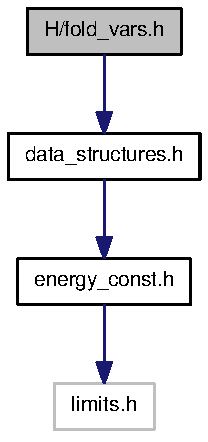
\includegraphics[width=68pt]{fold__vars_8h__incl}
\end{center}
\end{figure}
\subsection*{Functions}
\begin{DoxyCompactItemize}
\item 
void \hyperlink{fold__vars_8h_a4c3257186a796182462f18a5480ac8b3}{set\_\-model\_\-details} (\hyperlink{structmodel__detailsT}{model\_\-detailsT} $\ast$md)
\begin{DoxyCompactList}\small\item\em Set default model details. \item\end{DoxyCompactList}\end{DoxyCompactItemize}
\subsection*{Variables}
\begin{DoxyCompactItemize}
\item 
\hypertarget{fold__vars_8h_a0afc287c2464866d94858c39175154af}{
int \hyperlink{fold__vars_8h_a0afc287c2464866d94858c39175154af}{fold\_\-constrained}}
\label{fold__vars_8h_a0afc287c2464866d94858c39175154af}

\begin{DoxyCompactList}\small\item\em Global switch to activate/deactivate folding with structure constraints. \item\end{DoxyCompactList}\item 
int \hyperlink{fold__vars_8h_a097eccaabd6ae8b4fef83cccff85bb5d}{noLonelyPairs}
\begin{DoxyCompactList}\small\item\em Global switch to avoid/allow helices of length 1. \item\end{DoxyCompactList}\item 
int \hyperlink{fold__vars_8h_a72b511ed1201f7e23ec437e468790d74}{dangles}
\begin{DoxyCompactList}\small\item\em Switch the energy model for dangling end contributions (0, 1, 2, 3). \item\end{DoxyCompactList}\item 
\hypertarget{fold__vars_8h_abf380d09e4f1ab94fc6af57cf0ad5d32}{
int \hyperlink{fold__vars_8h_abf380d09e4f1ab94fc6af57cf0ad5d32}{noGU}}
\label{fold__vars_8h_abf380d09e4f1ab94fc6af57cf0ad5d32}

\begin{DoxyCompactList}\small\item\em Global switch to forbid/allow GU base pairs at all. \item\end{DoxyCompactList}\item 
\hypertarget{fold__vars_8h_aa8d1c7b92489179e1eafa562b7bdd259}{
int \hyperlink{fold__vars_8h_aa8d1c7b92489179e1eafa562b7bdd259}{no\_\-closingGU}}
\label{fold__vars_8h_aa8d1c7b92489179e1eafa562b7bdd259}

\begin{DoxyCompactList}\small\item\em GU allowed only inside stacks if set to 1. \item\end{DoxyCompactList}\item 
int \hyperlink{fold__vars_8h_a4f6265bdf0ead7ff4628a360adbfd77e}{tetra\_\-loop}
\begin{DoxyCompactList}\small\item\em Include special stabilizing energies for some tri-\/, tetra-\/ and hexa-\/loops;. \item\end{DoxyCompactList}\item 
int \hyperlink{fold__vars_8h_afb1ef1166da85092ae8a325e02dcae71}{energy\_\-set}
\begin{DoxyCompactList}\small\item\em 0 = BP; 1=any mit GC; 2=any mit AU-\/parameter \item\end{DoxyCompactList}\item 
int \hyperlink{fold__vars_8h_af9202a1a09f5828dc731e2d9a10fa111}{circ}
\begin{DoxyCompactList}\small\item\em backward compatibility variable. \item\end{DoxyCompactList}\item 
\hypertarget{fold__vars_8h_af2763d55a74663a5e60652b8880baa5b}{
int \hyperlink{fold__vars_8h_af2763d55a74663a5e60652b8880baa5b}{csv}}
\label{fold__vars_8h_af2763d55a74663a5e60652b8880baa5b}

\begin{DoxyCompactList}\small\item\em generate comma seperated output \item\end{DoxyCompactList}\item 
\hypertarget{fold__vars_8h_ac408868ba00671cbc7d1d535105af045}{
int \hyperlink{fold__vars_8h_ac408868ba00671cbc7d1d535105af045}{oldAliEn}}
\label{fold__vars_8h_ac408868ba00671cbc7d1d535105af045}

\begin{DoxyCompactList}\small\item\em use old alifold energies (with gaps) \item\end{DoxyCompactList}\item 
\hypertarget{fold__vars_8h_a0656afca1d2853f9ee6591172f5638de}{
int \hyperlink{fold__vars_8h_a0656afca1d2853f9ee6591172f5638de}{ribo}}
\label{fold__vars_8h_a0656afca1d2853f9ee6591172f5638de}

\begin{DoxyCompactList}\small\item\em use ribosum matrices \item\end{DoxyCompactList}\item 
\hypertarget{fold__vars_8h_a5dbaa0cca2c8c82048a0f0e38e164944}{
char $\ast$ \hyperlink{fold__vars_8h_a5dbaa0cca2c8c82048a0f0e38e164944}{RibosumFile}}
\label{fold__vars_8h_a5dbaa0cca2c8c82048a0f0e38e164944}

\begin{DoxyCompactList}\small\item\em warning this variable will vanish in the future ribosums will be compiled in instead \item\end{DoxyCompactList}\item 
char $\ast$ \hyperlink{fold__vars_8h_a2695d91cc535d09c2eae5c3884e2ec64}{nonstandards}
\begin{DoxyCompactList}\small\item\em contains allowed non standard base pairs \item\end{DoxyCompactList}\item 
double \hyperlink{fold__vars_8h_ab4b11c8d9c758430960896bc3fe82ead}{temperature}
\begin{DoxyCompactList}\small\item\em Rescale energy parameters to a temperature in degC. \item\end{DoxyCompactList}\item 
\hypertarget{fold__vars_8h_af349001ad3b4d008d0051d935b1b6261}{
int \hyperlink{fold__vars_8h_af349001ad3b4d008d0051d935b1b6261}{james\_\-rule}}
\label{fold__vars_8h_af349001ad3b4d008d0051d935b1b6261}

\begin{DoxyCompactList}\small\item\em interior loops of size 2 get energy 0.8Kcal and no mismatches, default 1 \item\end{DoxyCompactList}\item 
\hypertarget{fold__vars_8h_a80c3c5fd35e7479704cc91d2d0367743}{
int \hyperlink{fold__vars_8h_a80c3c5fd35e7479704cc91d2d0367743}{logML}}
\label{fold__vars_8h_a80c3c5fd35e7479704cc91d2d0367743}

\begin{DoxyCompactList}\small\item\em use logarithmic multiloop energy function \item\end{DoxyCompactList}\item 
int \hyperlink{fold__vars_8h_ab9b2c3a37a5516614c06d0ab54b97cda}{cut\_\-point}
\begin{DoxyCompactList}\small\item\em Marks the position (starting from 1) of the first nucleotide of the second molecule within the concatenated sequence. \item\end{DoxyCompactList}\item 
\hyperlink{structbondT}{bondT} $\ast$ \hyperlink{fold__vars_8h_a0244a629b5ab4f58b77590c3dfd130dc}{base\_\-pair}
\begin{DoxyCompactList}\small\item\em Contains a list of base pairs after a call to \hyperlink{fold_8h_aadafcb0f140795ae62e5ca027e335a9b}{fold()}. \item\end{DoxyCompactList}\item 
FLT\_\-OR\_\-DBL $\ast$ \hyperlink{fold__vars_8h_ac98ec419070aee6831b44e5c700f090f}{pr}
\begin{DoxyCompactList}\small\item\em A pointer to the base pair probability matrix. \item\end{DoxyCompactList}\item 
int $\ast$ \hyperlink{fold__vars_8h_a92089ae3a51b5d75a14ce9cc29cc8317}{iindx}
\begin{DoxyCompactList}\small\item\em index array to move through pr. \item\end{DoxyCompactList}\item 
double \hyperlink{fold__vars_8h_ad3b22044065acc6dee0af68931b52cfd}{pf\_\-scale}
\begin{DoxyCompactList}\small\item\em A scaling factor used by \hyperlink{part__func_8h_adc3db3d98742427e7001a7fd36ef28c2}{pf\_\-fold()} to avoid overflows. \item\end{DoxyCompactList}\item 
int \hyperlink{fold__vars_8h_ad512b5dd4dbec60faccfe137bb474489}{do\_\-backtrack}
\begin{DoxyCompactList}\small\item\em do backtracking, i.e. \item\end{DoxyCompactList}\item 
char \hyperlink{fold__vars_8h_a83bdb43472a259c71e69fa9f70f420c3}{backtrack\_\-type}
\begin{DoxyCompactList}\small\item\em A backtrack array marker for \hyperlink{inverse_8h_a7af026de55d4babad879f2c92559cbbc}{inverse\_\-fold()}. \item\end{DoxyCompactList}\end{DoxyCompactItemize}


\subsection{Detailed Description}
Here all all declarations of the global variables used throughout RNAlib. 

\subsection{Function Documentation}
\hypertarget{fold__vars_8h_a4c3257186a796182462f18a5480ac8b3}{
\index{fold\_\-vars.h@{fold\_\-vars.h}!set\_\-model\_\-details@{set\_\-model\_\-details}}
\index{set\_\-model\_\-details@{set\_\-model\_\-details}!fold_vars.h@{fold\_\-vars.h}}
\subsubsection[{set\_\-model\_\-details}]{\setlength{\rightskip}{0pt plus 5cm}void set\_\-model\_\-details ({\bf model\_\-detailsT} $\ast$ {\em md})}}
\label{fold__vars_8h_a4c3257186a796182462f18a5480ac8b3}


Set default model details. 

Use this function if you wish to initialize a \hyperlink{structmodel__detailsT}{model\_\-detailsT} data structure with its default values, i.e. the global model settings

\begin{DoxySeeAlso}{See also}

\end{DoxySeeAlso}

\begin{DoxyParams}{Parameters}
\item[{\em md}]A pointer to the data structure that shall be initialized \end{DoxyParams}


\subsection{Variable Documentation}
\hypertarget{fold__vars_8h_a097eccaabd6ae8b4fef83cccff85bb5d}{
\index{fold\_\-vars.h@{fold\_\-vars.h}!noLonelyPairs@{noLonelyPairs}}
\index{noLonelyPairs@{noLonelyPairs}!fold_vars.h@{fold\_\-vars.h}}
\subsubsection[{noLonelyPairs}]{\setlength{\rightskip}{0pt plus 5cm}int {\bf noLonelyPairs}}}
\label{fold__vars_8h_a097eccaabd6ae8b4fef83cccff85bb5d}


Global switch to avoid/allow helices of length 1. 

Disallow all pairs which can only occur as lonely pairs (i.e. as helix of length 1). This avoids lonely base pairs in the predicted structures in most cases. \hypertarget{fold__vars_8h_a72b511ed1201f7e23ec437e468790d74}{
\index{fold\_\-vars.h@{fold\_\-vars.h}!dangles@{dangles}}
\index{dangles@{dangles}!fold_vars.h@{fold\_\-vars.h}}
\subsubsection[{dangles}]{\setlength{\rightskip}{0pt plus 5cm}int {\bf dangles}}}
\label{fold__vars_8h_a72b511ed1201f7e23ec437e468790d74}


Switch the energy model for dangling end contributions (0, 1, 2, 3). 

If set to 0 no stabilizing energies are assigned to bases adjacent to helices in free ends and multiloops (so called dangling ends). Normally (dangles = 1) dangling end energies are assigned only to unpaired bases and a base cannot participate simultaneously in two dangling ends. In the partition function algorithm \hyperlink{part__func_8h_adc3db3d98742427e7001a7fd36ef28c2}{pf\_\-fold()} these checks are neglected. If \hyperlink{fold__vars_8h_a72b511ed1201f7e23ec437e468790d74}{dangles} is set to 2, all folding routines will follow this convention. This treatment of dangling ends gives more favorable energies to helices directly adjacent to one another, which can be beneficial since such helices often do engage in stabilizing interactions through co-\/axial stacking.\par
 If dangles = 3 co-\/axial stacking is explicitly included for adjacent helices in mutli-\/loops. The option affects only mfe folding and energy evaluation (\hyperlink{fold_8h_aadafcb0f140795ae62e5ca027e335a9b}{fold()} and \hyperlink{fold_8h_af93986cb3cb29770ec9cca69c9fab8cf}{energy\_\-of\_\-structure()}), as well as suboptimal folding (\hyperlink{subopt_8h_ac7f749cb177da547798509ebe021884c}{subopt()}) via re-\/evaluation of energies. Co-\/axial stacking with one intervening mismatch is not considered so far.

Default is 2 in most algorithms, partition function algorithms can only handle 0 and 2 \hypertarget{fold__vars_8h_a4f6265bdf0ead7ff4628a360adbfd77e}{
\index{fold\_\-vars.h@{fold\_\-vars.h}!tetra\_\-loop@{tetra\_\-loop}}
\index{tetra\_\-loop@{tetra\_\-loop}!fold_vars.h@{fold\_\-vars.h}}
\subsubsection[{tetra\_\-loop}]{\setlength{\rightskip}{0pt plus 5cm}int {\bf tetra\_\-loop}}}
\label{fold__vars_8h_a4f6265bdf0ead7ff4628a360adbfd77e}


Include special stabilizing energies for some tri-\/, tetra-\/ and hexa-\/loops;. 

default is 1. \hypertarget{fold__vars_8h_afb1ef1166da85092ae8a325e02dcae71}{
\index{fold\_\-vars.h@{fold\_\-vars.h}!energy\_\-set@{energy\_\-set}}
\index{energy\_\-set@{energy\_\-set}!fold_vars.h@{fold\_\-vars.h}}
\subsubsection[{energy\_\-set}]{\setlength{\rightskip}{0pt plus 5cm}int {\bf energy\_\-set}}}
\label{fold__vars_8h_afb1ef1166da85092ae8a325e02dcae71}


0 = BP; 1=any mit GC; 2=any mit AU-\/parameter 

If set to 1 or 2: fold sequences from an artificial alphabet ABCD..., where A pairs B, C pairs D, etc. using either GC (1) or AU parameters (2); default is 0, you probably don't want to change it. \hypertarget{fold__vars_8h_af9202a1a09f5828dc731e2d9a10fa111}{
\index{fold\_\-vars.h@{fold\_\-vars.h}!circ@{circ}}
\index{circ@{circ}!fold_vars.h@{fold\_\-vars.h}}
\subsubsection[{circ}]{\setlength{\rightskip}{0pt plus 5cm}int {\bf circ}}}
\label{fold__vars_8h_af9202a1a09f5828dc731e2d9a10fa111}


backward compatibility variable. 

. this does not effect anything \hypertarget{fold__vars_8h_a2695d91cc535d09c2eae5c3884e2ec64}{
\index{fold\_\-vars.h@{fold\_\-vars.h}!nonstandards@{nonstandards}}
\index{nonstandards@{nonstandards}!fold_vars.h@{fold\_\-vars.h}}
\subsubsection[{nonstandards}]{\setlength{\rightskip}{0pt plus 5cm}char$\ast$ {\bf nonstandards}}}
\label{fold__vars_8h_a2695d91cc535d09c2eae5c3884e2ec64}


contains allowed non standard base pairs 

Lists additional base pairs that will be allowed to form in addition to GC, CG, AU, UA, GU and UG. Nonstandard base pairs are given a stacking energy of 0. \hypertarget{fold__vars_8h_ab4b11c8d9c758430960896bc3fe82ead}{
\index{fold\_\-vars.h@{fold\_\-vars.h}!temperature@{temperature}}
\index{temperature@{temperature}!fold_vars.h@{fold\_\-vars.h}}
\subsubsection[{temperature}]{\setlength{\rightskip}{0pt plus 5cm}double {\bf temperature}}}
\label{fold__vars_8h_ab4b11c8d9c758430960896bc3fe82ead}


Rescale energy parameters to a temperature in degC. 

Default is 37C. You have to call the update\_\-...\_\-params() functions after changing this parameter. \hypertarget{fold__vars_8h_ab9b2c3a37a5516614c06d0ab54b97cda}{
\index{fold\_\-vars.h@{fold\_\-vars.h}!cut\_\-point@{cut\_\-point}}
\index{cut\_\-point@{cut\_\-point}!fold_vars.h@{fold\_\-vars.h}}
\subsubsection[{cut\_\-point}]{\setlength{\rightskip}{0pt plus 5cm}int {\bf cut\_\-point}}}
\label{fold__vars_8h_ab9b2c3a37a5516614c06d0ab54b97cda}


Marks the position (starting from 1) of the first nucleotide of the second molecule within the concatenated sequence. 

To evaluate the energy of a duplex structure (a structure formed by two strands), concatenate the to sequences and set it to the first base of the second strand in the concatenated sequence. The default value of -\/1 stands for single molecule folding. The cut\_\-point variable is also used by \hyperlink{PS__dot_8h_a0873c7cc4cd7a11c9a2cea19dde7e9c9}{PS\_\-rna\_\-plot()} and \hyperlink{PS__dot_8h_a689a97a7e3b8a2df14728b8204d9d57b}{PS\_\-dot\_\-plot()} to mark the chain break in postscript plots. \hypertarget{fold__vars_8h_a0244a629b5ab4f58b77590c3dfd130dc}{
\index{fold\_\-vars.h@{fold\_\-vars.h}!base\_\-pair@{base\_\-pair}}
\index{base\_\-pair@{base\_\-pair}!fold_vars.h@{fold\_\-vars.h}}
\subsubsection[{base\_\-pair}]{\setlength{\rightskip}{0pt plus 5cm}{\bf bondT}$\ast$ {\bf base\_\-pair}}}
\label{fold__vars_8h_a0244a629b5ab4f58b77590c3dfd130dc}


Contains a list of base pairs after a call to \hyperlink{fold_8h_aadafcb0f140795ae62e5ca027e335a9b}{fold()}. 

base\_\-pair\mbox{[}0\mbox{]}.i contains the total number of pairs. \begin{Desc}
\item[\hyperlink{deprecated__deprecated000008}{Deprecated}]Do not use this variable anymore! \end{Desc}
\hypertarget{fold__vars_8h_ac98ec419070aee6831b44e5c700f090f}{
\index{fold\_\-vars.h@{fold\_\-vars.h}!pr@{pr}}
\index{pr@{pr}!fold_vars.h@{fold\_\-vars.h}}
\subsubsection[{pr}]{\setlength{\rightskip}{0pt plus 5cm}FLT\_\-OR\_\-DBL$\ast$ {\bf pr}}}
\label{fold__vars_8h_ac98ec419070aee6831b44e5c700f090f}


A pointer to the base pair probability matrix. 

\begin{Desc}
\item[\hyperlink{deprecated__deprecated000009}{Deprecated}]Do not use this variable anymore! \end{Desc}
\hypertarget{fold__vars_8h_a92089ae3a51b5d75a14ce9cc29cc8317}{
\index{fold\_\-vars.h@{fold\_\-vars.h}!iindx@{iindx}}
\index{iindx@{iindx}!fold_vars.h@{fold\_\-vars.h}}
\subsubsection[{iindx}]{\setlength{\rightskip}{0pt plus 5cm}int$\ast$ {\bf iindx}}}
\label{fold__vars_8h_a92089ae3a51b5d75a14ce9cc29cc8317}


index array to move through pr. 

The probability for base i and j to form a pair is in pr\mbox{[}iindx\mbox{[}i\mbox{]}-\/j\mbox{]}. \begin{Desc}
\item[\hyperlink{deprecated__deprecated000010}{Deprecated}]Do not use this variable anymore! \end{Desc}
\hypertarget{fold__vars_8h_ad3b22044065acc6dee0af68931b52cfd}{
\index{fold\_\-vars.h@{fold\_\-vars.h}!pf\_\-scale@{pf\_\-scale}}
\index{pf\_\-scale@{pf\_\-scale}!fold_vars.h@{fold\_\-vars.h}}
\subsubsection[{pf\_\-scale}]{\setlength{\rightskip}{0pt plus 5cm}double {\bf pf\_\-scale}}}
\label{fold__vars_8h_ad3b22044065acc6dee0af68931b52cfd}


A scaling factor used by \hyperlink{part__func_8h_adc3db3d98742427e7001a7fd36ef28c2}{pf\_\-fold()} to avoid overflows. 

Should be set to approximately $exp{((-F/kT)/length)}$, where $F$ is an estimate for the ensemble free energy, for example the minimum free energy. You must call \hyperlink{part__func_8h_a384e927890f9c034ff09fa66da102d28}{update\_\-pf\_\-params()} after changing this parameter.\par
 If pf\_\-scale is -\/1 (the default) , an estimate will be provided automatically when computing partition functions, e.g. \hyperlink{part__func_8h_adc3db3d98742427e7001a7fd36ef28c2}{pf\_\-fold()} The automatic estimate is usually insufficient for sequences more than a few hundred bases long. \hypertarget{fold__vars_8h_ad512b5dd4dbec60faccfe137bb474489}{
\index{fold\_\-vars.h@{fold\_\-vars.h}!do\_\-backtrack@{do\_\-backtrack}}
\index{do\_\-backtrack@{do\_\-backtrack}!fold_vars.h@{fold\_\-vars.h}}
\subsubsection[{do\_\-backtrack}]{\setlength{\rightskip}{0pt plus 5cm}int {\bf do\_\-backtrack}}}
\label{fold__vars_8h_ad512b5dd4dbec60faccfe137bb474489}


do backtracking, i.e. 

compute secondary structures or base pair probabilities

If 0, do not calculate pair probabilities in \hyperlink{part__func_8h_adc3db3d98742427e7001a7fd36ef28c2}{pf\_\-fold()}; this is about twice as fast. Default is 1. \hypertarget{fold__vars_8h_a83bdb43472a259c71e69fa9f70f420c3}{
\index{fold\_\-vars.h@{fold\_\-vars.h}!backtrack\_\-type@{backtrack\_\-type}}
\index{backtrack\_\-type@{backtrack\_\-type}!fold_vars.h@{fold\_\-vars.h}}
\subsubsection[{backtrack\_\-type}]{\setlength{\rightskip}{0pt plus 5cm}char {\bf backtrack\_\-type}}}
\label{fold__vars_8h_a83bdb43472a259c71e69fa9f70f420c3}


A backtrack array marker for \hyperlink{inverse_8h_a7af026de55d4babad879f2c92559cbbc}{inverse\_\-fold()}. 

If set to 'C': force (1,N) to be paired, 'M' fold as if the sequence were inside a multi-\/loop. Otherwise ('F') the usual mfe structure is computed. 
\hypertarget{inverse_8h}{
\section{H/inverse.h File Reference}
\label{inverse_8h}\index{H/inverse.h@{H/inverse.h}}
}


Inverse folding routines.  


\subsection*{Functions}
\begin{DoxyCompactItemize}
\item 
float \hyperlink{inverse_8h_a7af026de55d4babad879f2c92559cbbc}{inverse\_\-fold} (char $\ast$start, const char $\ast$target)
\begin{DoxyCompactList}\small\item\em Find sequences with predefined structure. \item\end{DoxyCompactList}\item 
float \hyperlink{inverse_8h_aeef52ecbf2a2450ad585a344f9826806}{inverse\_\-pf\_\-fold} (char $\ast$start, const char $\ast$target)
\begin{DoxyCompactList}\small\item\em Find sequence that maximizes probability of a predefined structure. \item\end{DoxyCompactList}\end{DoxyCompactItemize}
\subsection*{Variables}
\begin{DoxyCompactItemize}
\item 
char $\ast$ \hyperlink{inverse_8h_a8f791e7740a5a28b9f6fafb4e60301d9}{symbolset}
\begin{DoxyCompactList}\small\item\em This global variable points to the allowed bases, initially \char`\"{}AUGC\char`\"{}. \item\end{DoxyCompactList}\item 
\hypertarget{inverse_8h_a7f17d3b169af048d32bb185039a9c09c}{
float \hyperlink{inverse_8h_a7f17d3b169af048d32bb185039a9c09c}{final\_\-cost}}
\label{inverse_8h_a7f17d3b169af048d32bb185039a9c09c}

\begin{DoxyCompactList}\small\item\em when to stop \hyperlink{inverse_8h_aeef52ecbf2a2450ad585a344f9826806}{inverse\_\-pf\_\-fold()} \item\end{DoxyCompactList}\item 
\hypertarget{inverse_8h_a7ec4ba51f86e1717a1e174264e4a75ce}{
int \hyperlink{inverse_8h_a7ec4ba51f86e1717a1e174264e4a75ce}{give\_\-up}}
\label{inverse_8h_a7ec4ba51f86e1717a1e174264e4a75ce}

\begin{DoxyCompactList}\small\item\em default 0: try to minimize structure distance even if no exact solution can be found \item\end{DoxyCompactList}\item 
\hypertarget{inverse_8h_afcfc65fba01b9cca5946726ed9057a63}{
int \hyperlink{inverse_8h_afcfc65fba01b9cca5946726ed9057a63}{inv\_\-verbose}}
\label{inverse_8h_afcfc65fba01b9cca5946726ed9057a63}

\begin{DoxyCompactList}\small\item\em print out substructure on which \hyperlink{inverse_8h_a7af026de55d4babad879f2c92559cbbc}{inverse\_\-fold()} fails \item\end{DoxyCompactList}\end{DoxyCompactItemize}


\subsection{Detailed Description}
Inverse folding routines. 

\subsection{Function Documentation}
\hypertarget{inverse_8h_a7af026de55d4babad879f2c92559cbbc}{
\index{inverse.h@{inverse.h}!inverse\_\-fold@{inverse\_\-fold}}
\index{inverse\_\-fold@{inverse\_\-fold}!inverse.h@{inverse.h}}
\subsubsection[{inverse\_\-fold}]{\setlength{\rightskip}{0pt plus 5cm}float inverse\_\-fold (char $\ast$ {\em start}, \/  const char $\ast$ {\em target})}}
\label{inverse_8h_a7af026de55d4babad879f2c92559cbbc}


Find sequences with predefined structure. 

This function searches for a sequence with minimum free energy structure provided in the parameter 'target', starting with sequence 'start'. It returns 0 if the search was successful, otherwise a structure distance in terms of the energy difference between the search result and the actual target 'target' is returned. The found sequence is returned in 'start'. If \hyperlink{inverse_8h_a7ec4ba51f86e1717a1e174264e4a75ce}{give\_\-up} is set to 1, the function will return as soon as it is clear that the search will be unsuccessful, this speeds up the algorithm if you are only interested in exact solutions.


\begin{DoxyParams}{Parameters}
\item[{\em start}]The start sequence 
\begin{DoxyParams}{Parameters}
\item[{\em target}]The target secondary structure in dot-\/bracket notation \begin{DoxyReturn}{Returns}
The distance to the target in case a search was unsuccessful, 0 otherwise 
\end{DoxyReturn}
\end{DoxyParams}
\end{DoxyParams}
\hypertarget{inverse_8h_aeef52ecbf2a2450ad585a344f9826806}{
\index{inverse.h@{inverse.h}!inverse\_\-pf\_\-fold@{inverse\_\-pf\_\-fold}}
\index{inverse\_\-pf\_\-fold@{inverse\_\-pf\_\-fold}!inverse.h@{inverse.h}}
\subsubsection[{inverse\_\-pf\_\-fold}]{\setlength{\rightskip}{0pt plus 5cm}float inverse\_\-pf\_\-fold (char $\ast$ {\em start}, \/  const char $\ast$ {\em target})}}
\label{inverse_8h_aeef52ecbf2a2450ad585a344f9826806}


Find sequence that maximizes probability of a predefined structure. 

This function searches for a sequence with maximum probability to fold into the provided structure 'target' using the partition function algorithm. It returns $-kT \cdot \log(p)$ where $p$ is the frequency of 'target' in the ensemble of possible structures. This is usually much slower than \hyperlink{inverse_8h_a7af026de55d4babad879f2c92559cbbc}{inverse\_\-fold()}.


\begin{DoxyParams}{Parameters}
\item[{\em start}]The start sequence 
\begin{DoxyParams}{Parameters}
\item[{\em target}]The target secondary structure in dot-\/bracket notation \begin{DoxyReturn}{Returns}
The distance to the target in case a search was unsuccessful, 0 otherwise 
\end{DoxyReturn}
\end{DoxyParams}
\end{DoxyParams}


\subsection{Variable Documentation}
\hypertarget{inverse_8h_a8f791e7740a5a28b9f6fafb4e60301d9}{
\index{inverse.h@{inverse.h}!symbolset@{symbolset}}
\index{symbolset@{symbolset}!inverse.h@{inverse.h}}
\subsubsection[{symbolset}]{\setlength{\rightskip}{0pt plus 5cm}char$\ast$ {\bf symbolset}}}
\label{inverse_8h_a8f791e7740a5a28b9f6fafb4e60301d9}


This global variable points to the allowed bases, initially \char`\"{}AUGC\char`\"{}. 

It can be used to design sequences from reduced alphabets. 
\hypertarget{Lfold_8h}{
\section{H/Lfold.h File Reference}
\label{Lfold_8h}\index{H/Lfold.h@{H/Lfold.h}}
}


Predicting local MFE structures of large sequences.  


\subsection*{Functions}
\begin{DoxyCompactItemize}
\item 
float \hyperlink{Lfold_8h_a16e5a70e60835bb969eaecbe6482f1be}{Lfold} (const char $\ast$string, char $\ast$structure, int maxdist)
\begin{DoxyCompactList}\small\item\em The local analog to \hyperlink{fold_8h_aadafcb0f140795ae62e5ca027e335a9b}{fold()}. \item\end{DoxyCompactList}\item 
float \hyperlink{Lfold_8h_a20a173a3cdb83f5d1778e36c1a6b1f2b}{aliLfold} (const char $\ast$$\ast$strings, char $\ast$structure, int maxdist)
\item 
float \hyperlink{Lfold_8h_ab6d79eecc180f586679f7b85cce5cbe9}{Lfoldz} (const char $\ast$string, char $\ast$structure, int maxdist, int zsc, double min\_\-z)
\end{DoxyCompactItemize}


\subsection{Detailed Description}
Predicting local MFE structures of large sequences. 

\subsection{Function Documentation}
\hypertarget{Lfold_8h_a16e5a70e60835bb969eaecbe6482f1be}{
\index{Lfold.h@{Lfold.h}!Lfold@{Lfold}}
\index{Lfold@{Lfold}!Lfold.h@{Lfold.h}}
\subsubsection[{Lfold}]{\setlength{\rightskip}{0pt plus 5cm}float Lfold (const char $\ast$ {\em string}, \/  char $\ast$ {\em structure}, \/  int {\em maxdist})}}
\label{Lfold_8h_a16e5a70e60835bb969eaecbe6482f1be}


The local analog to \hyperlink{fold_8h_aadafcb0f140795ae62e5ca027e335a9b}{fold()}. 

Computes the minimum free energy structure including only base pairs with a span smaller than 'maxdist'


\begin{DoxyParams}{Parameters}
\item[{\em string}]
\begin{DoxyParams}{Parameters}
\item[{\em structure}]
\begin{DoxyParams}{Parameters}
\item[{\em maxdist}]\end{DoxyParams}
\end{DoxyParams}
\end{DoxyParams}
\hypertarget{Lfold_8h_a20a173a3cdb83f5d1778e36c1a6b1f2b}{
\index{Lfold.h@{Lfold.h}!aliLfold@{aliLfold}}
\index{aliLfold@{aliLfold}!Lfold.h@{Lfold.h}}
\subsubsection[{aliLfold}]{\setlength{\rightskip}{0pt plus 5cm}float aliLfold (const char $\ast$$\ast$ {\em strings}, \/  char $\ast$ {\em structure}, \/  int {\em maxdist})}}
\label{Lfold_8h_a20a173a3cdb83f5d1778e36c1a6b1f2b}

\begin{DoxyParams}{Parameters}
\item[{\em strings}]
\begin{DoxyParams}{Parameters}
\item[{\em structure}]
\begin{DoxyParams}{Parameters}
\item[{\em maxdist}]\begin{DoxyReturn}{Returns}

\end{DoxyReturn}
\end{DoxyParams}
\end{DoxyParams}
\end{DoxyParams}
\hypertarget{Lfold_8h_ab6d79eecc180f586679f7b85cce5cbe9}{
\index{Lfold.h@{Lfold.h}!Lfoldz@{Lfoldz}}
\index{Lfoldz@{Lfoldz}!Lfold.h@{Lfold.h}}
\subsubsection[{Lfoldz}]{\setlength{\rightskip}{0pt plus 5cm}float Lfoldz (const char $\ast$ {\em string}, \/  char $\ast$ {\em structure}, \/  int {\em maxdist}, \/  int {\em zsc}, \/  double {\em min\_\-z})}}
\label{Lfold_8h_ab6d79eecc180f586679f7b85cce5cbe9}

\begin{DoxyParams}{Parameters}
\item[{\em string}]
\begin{DoxyParams}{Parameters}
\item[{\em structure}]
\begin{DoxyParams}{Parameters}
\item[{\em maxdist}]
\begin{DoxyParams}{Parameters}
\item[{\em zsc}]
\begin{DoxyParams}{Parameters}
\item[{\em min\_\-z}]\end{DoxyParams}
\end{DoxyParams}
\end{DoxyParams}
\end{DoxyParams}
\end{DoxyParams}

\hypertarget{loop__energies_8h}{
\section{H/loop\_\-energies.h File Reference}
\label{loop__energies_8h}\index{H/loop\_\-energies.h@{H/loop\_\-energies.h}}
}


Energy evaluation for MFE and partition function calculations.  


Include dependency graph for loop\_\-energies.h:\nopagebreak
\begin{figure}[H]
\begin{center}
\leavevmode
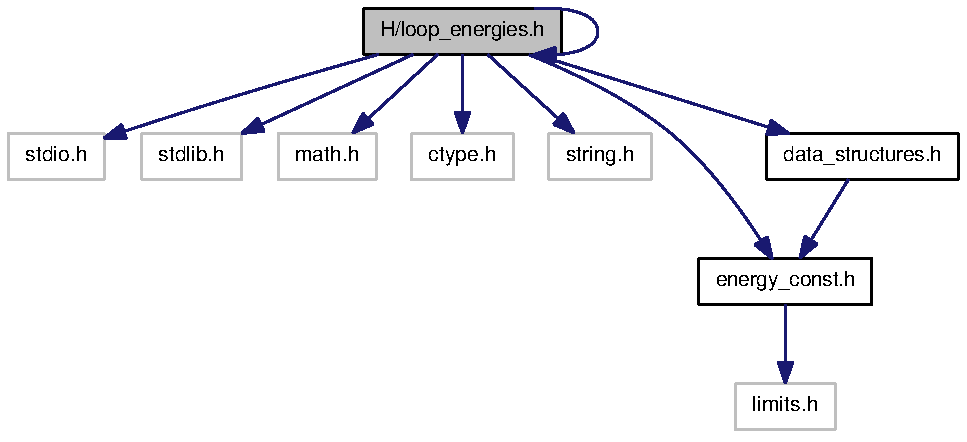
\includegraphics[width=250pt]{loop__energies_8h__incl}
\end{center}
\end{figure}
This graph shows which files directly or indirectly include this file:\nopagebreak
\begin{figure}[H]
\begin{center}
\leavevmode
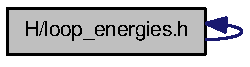
\includegraphics[width=78pt]{loop__energies_8h__dep__incl}
\end{center}
\end{figure}
\subsection*{Functions}
\begin{DoxyCompactItemize}
\item 
PRIVATE int \hyperlink{loop__energies_8h_a3e5ad89f451254b1fe366d77aa8ff7bd}{E\_\-IntLoop} (int n1, int n2, int type, int type\_\-2, int si1, int sj1, int sp1, int sq1, \hyperlink{structparamT}{paramT} $\ast$P)
\item 
PRIVATE int \hyperlink{loop__energies_8h_aa362183cf6db89a10cdb0f5c4bd180c6}{E\_\-Hairpin} (int size, int type, int si1, int sj1, const char $\ast$string, \hyperlink{structparamT}{paramT} $\ast$P)
\item 
PRIVATE int \hyperlink{loop__energies_8h_af5a6594eba9b2622cb47076650c69819}{E\_\-Stem} (int type, int si1, int sj1, int extLoop, \hyperlink{structparamT}{paramT} $\ast$P)
\item 
PRIVATE double \hyperlink{loop__energies_8h_a76cc24ec96199e04beddad13e7891e21}{exp\_\-E\_\-Stem} (int type, int si1, int sj1, int extLoop, \hyperlink{structpf__paramT}{pf\_\-paramT} $\ast$P)
\item 
PRIVATE double \hyperlink{loop__energies_8h_a0e128184bb097dc2da33706f33b555a6}{exp\_\-E\_\-Hairpin} (int u, int type, short si1, short sj1, const char $\ast$string, \hyperlink{structpf__paramT}{pf\_\-paramT} $\ast$P)
\item 
PRIVATE double \hyperlink{loop__energies_8h_aa5e98e524e2a41e290b942b09544bc9e}{exp\_\-E\_\-IntLoop} (int u1, int u2, int type, int type2, short si1, short sj1, short sp1, short sq1, \hyperlink{structpf__paramT}{pf\_\-paramT} $\ast$P)
\end{DoxyCompactItemize}


\subsection{Detailed Description}
Energy evaluation for MFE and partition function calculations. This file contains functions for the calculation of the free energy $\Delta G$ of a hairpin-\/ \mbox{[} \hyperlink{loop__energies_8h_aa362183cf6db89a10cdb0f5c4bd180c6}{E\_\-Hairpin()} \mbox{]} or interior-\/loop \mbox{[} \hyperlink{loop__energies_8h_a3e5ad89f451254b1fe366d77aa8ff7bd}{E\_\-IntLoop()}\mbox{]} .\par
 The unit of the free energy returned is $10^{-2} * \mathrm{kcal}/\mathrm{mol}$  

In case of computing the partition function, this file also supplies functions which return the Boltzmann weights $e^{-\Delta G/kT} $ for a hairpin-\/ \mbox{[} \hyperlink{loop__energies_8h_a0e128184bb097dc2da33706f33b555a6}{exp\_\-E\_\-Hairpin()} \mbox{]} or interior-\/loop \mbox{[} \hyperlink{loop__energies_8h_aa5e98e524e2a41e290b942b09544bc9e}{exp\_\-E\_\-IntLoop()} \mbox{]}.  

\subsection{Function Documentation}
\hypertarget{loop__energies_8h_a3e5ad89f451254b1fe366d77aa8ff7bd}{
\index{loop\_\-energies.h@{loop\_\-energies.h}!E\_\-IntLoop@{E\_\-IntLoop}}
\index{E\_\-IntLoop@{E\_\-IntLoop}!loop_energies.h@{loop\_\-energies.h}}
\subsubsection[{E\_\-IntLoop}]{\setlength{\rightskip}{0pt plus 5cm}PRIVATE int E\_\-IntLoop (int {\em n1}, \/  int {\em n2}, \/  int {\em type}, \/  int {\em type\_\-2}, \/  int {\em si1}, \/  int {\em sj1}, \/  int {\em sp1}, \/  int {\em sq1}, \/  {\bf paramT} $\ast$ {\em P})}}
\label{loop__energies_8h_a3e5ad89f451254b1fe366d77aa8ff7bd}
\subsubsection*{Compute the Energy of an interior-\/loop}

This function computes the free energy $\Delta G$ of an interior-\/loop with the following structure: \par
 
\begin{DoxyPre}
        3'  5'
        |   |
        U - V
    a\_n       b\_1
     .        .
     .        .
     .        .
    a\_1       b\_m
        X - Y
        |   |
        5'  3'
  \end{DoxyPre}
 This general structure depicts an interior-\/loop that is closed by the base pair (X,Y). The enclosed base pair is (V,U) which leaves the unpaired bases a\_\-1-\/a\_\-n and b\_\-1-\/b\_\-n that constitute the loop. In this example, the length of the interior-\/loop is $(n+m)$ where n or m may be 0 resulting in a bulge-\/loop or base pair stack. The mismatching nucleotides for the closing pair (X,Y) are:\par
 5'-\/mismatch: a\_\-1\par
 3'-\/mismatch: b\_\-m\par
 and for the enclosed base pair (V,U):\par
 5'-\/mismatch: b\_\-1\par
 3'-\/mismatch: a\_\-n\par
 \begin{DoxyNote}{Note}
Base pairs are always denoted in 5'-\/$>$3' direction. Thus the enclosed base pair must be 'turned arround' when evaluating the free energy of the interior-\/loop 
\end{DoxyNote}
\begin{DoxySeeAlso}{See also}
\hyperlink{params_8h_a527ef619cd8210b84d5d53be1e0e29b6}{scale\_\-parameters()} 

\hyperlink{structparamT}{paramT} 
\end{DoxySeeAlso}
\begin{DoxyNote}{Note}
This function is threadsafe
\end{DoxyNote}

\begin{DoxyParams}{Parameters}
\item[{\em n1}]The size of the 'left'-\/loop (number of unpaired nucleotides) 
\begin{DoxyParams}{Parameters}
\item[{\em n2}]The size of the 'right'-\/loop (number of unpaired nucleotides) 
\begin{DoxyParams}{Parameters}
\item[{\em type}]The pair type of the base pair closing the interior loop 
\begin{DoxyParams}{Parameters}
\item[{\em type\_\-2}]The pair type of the enclosed base pair 
\begin{DoxyParams}{Parameters}
\item[{\em si1}]The 5'-\/mismatching nucleotide of the closing pair 
\begin{DoxyParams}{Parameters}
\item[{\em sj1}]The 3'-\/mismatching nucleotide of the closing pair 
\begin{DoxyParams}{Parameters}
\item[{\em sp1}]The 3'-\/mismatching nucleotide of the enclosed pair 
\begin{DoxyParams}{Parameters}
\item[{\em sq1}]The 5'-\/mismatching nucleotide of the enclosed pair 
\begin{DoxyParams}{Parameters}
\item[{\em P}]The datastructure containing scaled energy parameters \begin{DoxyReturn}{Returns}
The Free energy of the Interior-\/loop in dcal/mol 
\end{DoxyReturn}
\end{DoxyParams}
\end{DoxyParams}
\end{DoxyParams}
\end{DoxyParams}
\end{DoxyParams}
\end{DoxyParams}
\end{DoxyParams}
\end{DoxyParams}
\end{DoxyParams}
\hypertarget{loop__energies_8h_aa362183cf6db89a10cdb0f5c4bd180c6}{
\index{loop\_\-energies.h@{loop\_\-energies.h}!E\_\-Hairpin@{E\_\-Hairpin}}
\index{E\_\-Hairpin@{E\_\-Hairpin}!loop_energies.h@{loop\_\-energies.h}}
\subsubsection[{E\_\-Hairpin}]{\setlength{\rightskip}{0pt plus 5cm}PRIVATE int E\_\-Hairpin (int {\em size}, \/  int {\em type}, \/  int {\em si1}, \/  int {\em sj1}, \/  const char $\ast$ {\em string}, \/  {\bf paramT} $\ast$ {\em P})}}
\label{loop__energies_8h_aa362183cf6db89a10cdb0f5c4bd180c6}
\subsubsection*{Compute the Energy of a hairpin-\/loop}

To evaluate the free energy of a hairpin-\/loop, several parameters have to be known. A general hairpin-\/loop has this structure:\par
 
\begin{DoxyPre}
        a3 a4
      a2     a5
      a1     a6
        X - Y
        |   |
        5'  3'
  \end{DoxyPre}
 where X-\/Y marks the closing pair \mbox{[}e.g. a {\bfseries (G,C)} pair\mbox{]}. The length of this loop is 6 as there are six unpaired nucleotides (a1-\/a6) enclosed by (X,Y). The 5' mismatching nucleotide is a1 while the 3' mismatch is a6. The nucleotide sequence of this loop is "a1.a2.a3.a4.a5.a6" \par
 \begin{DoxyNote}{Note}
The parameter sequence should contain the sequence of the loop in capital letters of the nucleic acid alphabet if the loop size is below 7. This is useful for unusually stable tri-\/, tetra-\/ and hexa-\/loops which are treated differently (based on experimental data) if they are tabulated. 
\end{DoxyNote}
\begin{DoxySeeAlso}{See also}
\hyperlink{params_8h_a527ef619cd8210b84d5d53be1e0e29b6}{scale\_\-parameters()} 

\hyperlink{structparamT}{paramT} 
\end{DoxySeeAlso}
\begin{DoxyWarning}{Warning}
Not (really) thread safe! A threadsafe implementation will replace this function in a future release!\par
 Energy evaluation may change due to updates in global variable \char`\"{}tetra\_\-loop\char`\"{}
\end{DoxyWarning}

\begin{DoxyParams}{Parameters}
\item[{\em size}]The size of the loop (number of unpaired nucleotides) 
\begin{DoxyParams}{Parameters}
\item[{\em type}]The pair type of the base pair closing the hairpin 
\begin{DoxyParams}{Parameters}
\item[{\em si1}]The 5'-\/mismatching nucleotide 
\begin{DoxyParams}{Parameters}
\item[{\em sj1}]The 3'-\/mismatching nucleotide 
\begin{DoxyParams}{Parameters}
\item[{\em string}]The sequence of the loop 
\begin{DoxyParams}{Parameters}
\item[{\em P}]The datastructure containing scaled energy parameters \begin{DoxyReturn}{Returns}
The Free energy of the Hairpin-\/loop in dcal/mol 
\end{DoxyReturn}
\end{DoxyParams}
\end{DoxyParams}
\end{DoxyParams}
\end{DoxyParams}
\end{DoxyParams}
\end{DoxyParams}
\hypertarget{loop__energies_8h_af5a6594eba9b2622cb47076650c69819}{
\index{loop\_\-energies.h@{loop\_\-energies.h}!E\_\-Stem@{E\_\-Stem}}
\index{E\_\-Stem@{E\_\-Stem}!loop_energies.h@{loop\_\-energies.h}}
\subsubsection[{E\_\-Stem}]{\setlength{\rightskip}{0pt plus 5cm}PRIVATE int E\_\-Stem (int {\em type}, \/  int {\em si1}, \/  int {\em sj1}, \/  int {\em extLoop}, \/  {\bf paramT} $\ast$ {\em P})}}
\label{loop__energies_8h_af5a6594eba9b2622cb47076650c69819}
\subsubsection*{Compute the energy contribution of a stem branching off a loop-\/region}

This function computes the energy contribution of a stem that branches off a loop region. This can be the case in multiloops, when a stem branching off increases the degree of the loop but also {\itshape immediately interior base pairs\/} of an exterior loop contribute free energy. To switch the bahavior of the function according to the evaluation of a multiloop-\/ or exterior-\/loop-\/stem, you pass the flag 'extLoop'. The returned energy contribution consists of a TerminalAU penalty if the pair type is greater than 2, dangling end contributions of mismatching nucleotides adjacent to the stem if only one of the si1, sj1 parameters is greater than 0 and mismatch energies if both mismatching nucleotides are positive values. Thus, to avoid incooperating dangling end or mismatch energies just pass a negative number, e.g. -\/1 to the mismatch argument.

This is an illustration of how the energy contribution is assembled: 
\begin{DoxyPre}
        3'  5'
        |   |
        X - Y
  5'-si1     sj1-3'
  \end{DoxyPre}


Here, (X,Y) is the base pair that closes the stem that branches off a loop region. The nucleotides si1 and sj1 are the 5'-\/ and 3'-\/ mismatches, respectively. If the base pair type of (X,Y) is greater than 2 (i.e. an A-\/U or G-\/U pair, the TerminalAU penalty will be included in the energy contribution returned. If si1 and sj1 are both nonnegative numbers, mismatch energies will also be included. If one of sij or sj1 is a negtive value, only 5' or 3' dangling end contributions are taken into account. To prohibit any of these mismatch contributions to be incoorporated, just pass a negative number to both, si1 and sj1. In case the argument extLoop is 0, the returned energy contribution also includes the {\itshape internal-\/loop-\/penalty\/} of a multiloop stem with closing pair type.

\begin{DoxySeeAlso}{See also}
E\_\-MLstem() 

E\_\-ExtLoop() 
\end{DoxySeeAlso}
\begin{DoxyNote}{Note}
This function is threadsafe
\end{DoxyNote}

\begin{DoxyParams}{Parameters}
\item[{\em type}]The pair type of the first base pair un the stem 
\begin{DoxyParams}{Parameters}
\item[{\em si1}]The 5'-\/mismatching nucleotide 
\begin{DoxyParams}{Parameters}
\item[{\em sj1}]The 3'-\/mismatching nucleotide 
\begin{DoxyParams}{Parameters}
\item[{\em extLoop}]A flag that indicates whether the contribution reflects the one of an exterior loop or not 
\begin{DoxyParams}{Parameters}
\item[{\em P}]The datastructure containing scaled energy parameters \begin{DoxyReturn}{Returns}
The Free energy of the branch off the loop in dcal/mol 
\end{DoxyReturn}
\end{DoxyParams}
\end{DoxyParams}
\end{DoxyParams}
\end{DoxyParams}
\end{DoxyParams}
\hypertarget{loop__energies_8h_a76cc24ec96199e04beddad13e7891e21}{
\index{loop\_\-energies.h@{loop\_\-energies.h}!exp\_\-E\_\-Stem@{exp\_\-E\_\-Stem}}
\index{exp\_\-E\_\-Stem@{exp\_\-E\_\-Stem}!loop_energies.h@{loop\_\-energies.h}}
\subsubsection[{exp\_\-E\_\-Stem}]{\setlength{\rightskip}{0pt plus 5cm}PRIVATE double exp\_\-E\_\-Stem (int {\em type}, \/  int {\em si1}, \/  int {\em sj1}, \/  int {\em extLoop}, \/  {\bf pf\_\-paramT} $\ast$ {\em P})}}
\label{loop__energies_8h_a76cc24ec96199e04beddad13e7891e21}
\subsubsection*{Compute the Boltzmann weighted energy contribution of a stem branching off a loop-\/region}

This is the partition function variant of \hyperlink{loop__energies_8h_af5a6594eba9b2622cb47076650c69819}{E\_\-Stem()} \begin{DoxySeeAlso}{See also}
\hyperlink{loop__energies_8h_af5a6594eba9b2622cb47076650c69819}{E\_\-Stem()} 
\end{DoxySeeAlso}
\begin{DoxyNote}{Note}
This function is threadsafe
\end{DoxyNote}
\begin{DoxyReturn}{Returns}
The Boltzmann weighted energy contribution of the branch off the loop 
\end{DoxyReturn}
\hypertarget{loop__energies_8h_a0e128184bb097dc2da33706f33b555a6}{
\index{loop\_\-energies.h@{loop\_\-energies.h}!exp\_\-E\_\-Hairpin@{exp\_\-E\_\-Hairpin}}
\index{exp\_\-E\_\-Hairpin@{exp\_\-E\_\-Hairpin}!loop_energies.h@{loop\_\-energies.h}}
\subsubsection[{exp\_\-E\_\-Hairpin}]{\setlength{\rightskip}{0pt plus 5cm}PRIVATE double exp\_\-E\_\-Hairpin (int {\em u}, \/  int {\em type}, \/  short {\em si1}, \/  short {\em sj1}, \/  const char $\ast$ {\em string}, \/  {\bf pf\_\-paramT} $\ast$ {\em P})}}
\label{loop__energies_8h_a0e128184bb097dc2da33706f33b555a6}
\subsubsection*{Compute Boltzmann weight $e^{-\Delta G/kT} $ of a hairpin loop}

multiply by scale\mbox{[}u+2\mbox{]} \begin{DoxySeeAlso}{See also}
\hyperlink{params_8h_ab85f6b6da051f380371deb0d8921bdba}{get\_\-scaled\_\-pf\_\-parameters()} 

\hyperlink{structpf__paramT}{pf\_\-paramT} 

\hyperlink{loop__energies_8h_aa362183cf6db89a10cdb0f5c4bd180c6}{E\_\-Hairpin()} 
\end{DoxySeeAlso}
\begin{DoxyWarning}{Warning}
Not (really) thread safe! A threadsafe implementation will replace this function in a future release!\par
 Energy evaluation may change due to updates in global variable \char`\"{}tetra\_\-loop\char`\"{}
\end{DoxyWarning}

\begin{DoxyParams}{Parameters}
\item[{\em u}]The size of the loop (number of unpaired nucleotides) 
\begin{DoxyParams}{Parameters}
\item[{\em type}]The pair type of the base pair closing the hairpin 
\begin{DoxyParams}{Parameters}
\item[{\em si1}]The 5'-\/mismatching nucleotide 
\begin{DoxyParams}{Parameters}
\item[{\em sj1}]The 3'-\/mismatching nucleotide 
\begin{DoxyParams}{Parameters}
\item[{\em string}]The sequence of the loop 
\begin{DoxyParams}{Parameters}
\item[{\em P}]The datastructure containing scaled Boltzmann weights of the energy parameters \begin{DoxyReturn}{Returns}
The Boltzmann weight of the Hairpin-\/loop 
\end{DoxyReturn}
\end{DoxyParams}
\end{DoxyParams}
\end{DoxyParams}
\end{DoxyParams}
\end{DoxyParams}
\end{DoxyParams}
\hypertarget{loop__energies_8h_aa5e98e524e2a41e290b942b09544bc9e}{
\index{loop\_\-energies.h@{loop\_\-energies.h}!exp\_\-E\_\-IntLoop@{exp\_\-E\_\-IntLoop}}
\index{exp\_\-E\_\-IntLoop@{exp\_\-E\_\-IntLoop}!loop_energies.h@{loop\_\-energies.h}}
\subsubsection[{exp\_\-E\_\-IntLoop}]{\setlength{\rightskip}{0pt plus 5cm}PRIVATE double exp\_\-E\_\-IntLoop (int {\em u1}, \/  int {\em u2}, \/  int {\em type}, \/  int {\em type2}, \/  short {\em si1}, \/  short {\em sj1}, \/  short {\em sp1}, \/  short {\em sq1}, \/  {\bf pf\_\-paramT} $\ast$ {\em P})}}
\label{loop__energies_8h_aa5e98e524e2a41e290b942b09544bc9e}
\subsubsection*{Compute Boltzmann weight $e^{-\Delta G/kT} $ of interior loop}

multiply by scale\mbox{[}u1+u2+2\mbox{]} for scaling \begin{DoxySeeAlso}{See also}
\hyperlink{params_8h_ab85f6b6da051f380371deb0d8921bdba}{get\_\-scaled\_\-pf\_\-parameters()} 

\hyperlink{structpf__paramT}{pf\_\-paramT} 

\hyperlink{loop__energies_8h_a3e5ad89f451254b1fe366d77aa8ff7bd}{E\_\-IntLoop()} 
\end{DoxySeeAlso}
\begin{DoxyNote}{Note}
This function is threadsafe
\end{DoxyNote}

\begin{DoxyParams}{Parameters}
\item[{\em u1}]The size of the 'left'-\/loop (number of unpaired nucleotides) 
\begin{DoxyParams}{Parameters}
\item[{\em u2}]The size of the 'right'-\/loop (number of unpaired nucleotides) 
\begin{DoxyParams}{Parameters}
\item[{\em type}]The pair type of the base pair closing the interior loop 
\begin{DoxyParams}{Parameters}
\item[{\em type2}]The pair type of the enclosed base pair 
\begin{DoxyParams}{Parameters}
\item[{\em si1}]The 5'-\/mismatching nucleotide of the closing pair 
\begin{DoxyParams}{Parameters}
\item[{\em sj1}]The 3'-\/mismatching nucleotide of the closing pair 
\begin{DoxyParams}{Parameters}
\item[{\em sp1}]The 3'-\/mismatching nucleotide of the enclosed pair 
\begin{DoxyParams}{Parameters}
\item[{\em sq1}]The 5'-\/mismatching nucleotide of the enclosed pair 
\begin{DoxyParams}{Parameters}
\item[{\em P}]The datastructure containing scaled Boltzmann weights of the energy parameters \begin{DoxyReturn}{Returns}
The Boltzmann weight of the Interior-\/loop 
\end{DoxyReturn}
\end{DoxyParams}
\end{DoxyParams}
\end{DoxyParams}
\end{DoxyParams}
\end{DoxyParams}
\end{DoxyParams}
\end{DoxyParams}
\end{DoxyParams}
\end{DoxyParams}

\hypertarget{LPfold_8h}{
\section{H/LPfold.h File Reference}
\label{LPfold_8h}\index{H/LPfold.h@{H/LPfold.h}}
}


Function declarations of partition function variants of the Lfold algorithm.  


Include dependency graph for LPfold.h:\nopagebreak
\begin{figure}[H]
\begin{center}
\leavevmode
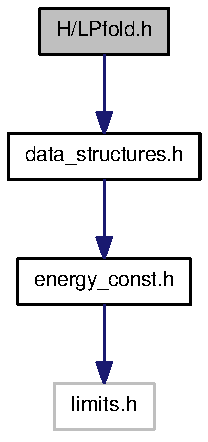
\includegraphics[width=68pt]{LPfold_8h__incl}
\end{center}
\end{figure}
\subsection*{Functions}
\begin{DoxyCompactItemize}
\item 
void \hyperlink{LPfold_8h_a5a019014d37fe6105131dfc2fc447880}{update\_\-pf\_\-paramsLP} (int length)
\item 
\hyperlink{structplist}{plist} $\ast$ \hyperlink{LPfold_8h_aa1ecd401617ebc748a0220026543c777}{pfl\_\-fold} (char $\ast$sequence, int winSize, int pairSize, float cutoffb, double $\ast$$\ast$pU, struct \hyperlink{structplist}{plist} $\ast$$\ast$dpp2, FILE $\ast$pUfp, FILE $\ast$spup)
\begin{DoxyCompactList}\small\item\em Compute partition functions for locally stable secondary structures {\bfseries (berni! update me)} \item\end{DoxyCompactList}\item 
void \hyperlink{LPfold_8h_a0bcb751860bbf34e3dfee8c2fbdb3ef3}{putoutpU\_\-prob} (double $\ast$$\ast$pU, int length, int ulength, FILE $\ast$fp, int energies)
\begin{DoxyCompactList}\small\item\em Writes the unpaired probabilities (pU) or opening energies into a file. \item\end{DoxyCompactList}\item 
void \hyperlink{LPfold_8h_a9acb00ee10e96b1ca4ea394cd8bcec75}{putoutpU\_\-prob\_\-bin} (double $\ast$$\ast$pU, int length, int ulength, FILE $\ast$fp, int energies)
\begin{DoxyCompactList}\small\item\em Writes the unpaired probabilities (pU) or opening energies into a binary file. \item\end{DoxyCompactList}\item 
void \hyperlink{LPfold_8h_ae85bf55053e9fb295208be322e0fa07a}{init\_\-pf\_\-foldLP} (int length)
\begin{DoxyCompactList}\small\item\em Dunno if this function was ever used by external programs linking to RNAlib, but it was declared PUBLIC before. \item\end{DoxyCompactList}\end{DoxyCompactItemize}


\subsection{Detailed Description}
Function declarations of partition function variants of the Lfold algorithm. 

\subsection{Function Documentation}
\hypertarget{LPfold_8h_a5a019014d37fe6105131dfc2fc447880}{
\index{LPfold.h@{LPfold.h}!update\_\-pf\_\-paramsLP@{update\_\-pf\_\-paramsLP}}
\index{update\_\-pf\_\-paramsLP@{update\_\-pf\_\-paramsLP}!LPfold.h@{LPfold.h}}
\subsubsection[{update\_\-pf\_\-paramsLP}]{\setlength{\rightskip}{0pt plus 5cm}void update\_\-pf\_\-paramsLP (int {\em length})}}
\label{LPfold_8h_a5a019014d37fe6105131dfc2fc447880}

\begin{DoxyParams}{Parameters}
\item[{\em length}]\end{DoxyParams}
\hypertarget{LPfold_8h_aa1ecd401617ebc748a0220026543c777}{
\index{LPfold.h@{LPfold.h}!pfl\_\-fold@{pfl\_\-fold}}
\index{pfl\_\-fold@{pfl\_\-fold}!LPfold.h@{LPfold.h}}
\subsubsection[{pfl\_\-fold}]{\setlength{\rightskip}{0pt plus 5cm}{\bf plist}$\ast$ pfl\_\-fold (char $\ast$ {\em sequence}, \/  int {\em winSize}, \/  int {\em pairSize}, \/  float {\em cutoffb}, \/  double $\ast$$\ast$ {\em pU}, \/  struct {\bf plist} $\ast$$\ast$ {\em dpp2}, \/  FILE $\ast$ {\em pUfp}, \/  FILE $\ast$ {\em spup})}}
\label{LPfold_8h_aa1ecd401617ebc748a0220026543c777}


Compute partition functions for locally stable secondary structures {\bfseries (berni! update me)} 

pfl\_\-fold computes partition functions for every window of size 'winSize' possible in a RNA molecule, allowing only pairs with a span smaller than 'pairSize'. It returns the mean pair probabilities averaged over all windows containing the pair in 'pl'. 'winSize' should always be $>$= 'pairSize'. Note that in contrast to \hyperlink{Lfold_8h_a16e5a70e60835bb969eaecbe6482f1be}{Lfold()}, bases outside of the window do not influence the structure at all. Only probabilities higher than 'cutoffb' are kept.

If 'pU' is supplied (i.e is not the NULL pointer), \hyperlink{LPfold_8h_aa1ecd401617ebc748a0220026543c777}{pfl\_\-fold()} will also compute the mean probability that regions of length 'u' and smaller are unpaired. The parameter 'u' is supplied in 'pup\mbox{[}0\mbox{]}\mbox{[}0\mbox{]}'. On return the 'pup' array will contain these probabilities, with the entry on 'pup\mbox{[}x\mbox{]}\mbox{[}y\mbox{]}' containing the mean probability that x and the y-\/1 preceding bases are unpaired. The 'pU' array needs to be large enough to hold n+1 float$\ast$ entries, where n is the sequence length.

If an array dpp2 is supplied, the probability of base pair (i,j) given that there already exists a base pair (i+1,j-\/1) is also computed and saved in this array. If pUfp is given (i.e. not NULL), pU is not saved but put out imediately. If spup is given (i.e. is not NULL), the pair probabilities in pl are not saved but put out imediately. 
\begin{DoxyParams}{Parameters}
\item[{\em sequence}]RNA sequence 
\begin{DoxyParams}{Parameters}
\item[{\em winSize}]size of the window 
\begin{DoxyParams}{Parameters}
\item[{\em pairSize}]maximum size of base pair 
\begin{DoxyParams}{Parameters}
\item[{\em cutoffb}]cutoffb for base pairs 
\begin{DoxyParams}{Parameters}
\item[{\em pU}]array holding all unpaired probabilities 
\begin{DoxyParams}{Parameters}
\item[{\em dpp2}]array of dependent pair probabilities 
\begin{DoxyParams}{Parameters}
\item[{\em pUfp}]file pointer for pU 
\begin{DoxyParams}{Parameters}
\item[{\em spup}]file pointer for pair probabilities \begin{DoxyReturn}{Returns}
list of pair probabilities 
\end{DoxyReturn}
\end{DoxyParams}
\end{DoxyParams}
\end{DoxyParams}
\end{DoxyParams}
\end{DoxyParams}
\end{DoxyParams}
\end{DoxyParams}
\end{DoxyParams}
\hypertarget{LPfold_8h_a0bcb751860bbf34e3dfee8c2fbdb3ef3}{
\index{LPfold.h@{LPfold.h}!putoutpU\_\-prob@{putoutpU\_\-prob}}
\index{putoutpU\_\-prob@{putoutpU\_\-prob}!LPfold.h@{LPfold.h}}
\subsubsection[{putoutpU\_\-prob}]{\setlength{\rightskip}{0pt plus 5cm}void putoutpU\_\-prob (double $\ast$$\ast$ {\em pU}, \/  int {\em length}, \/  int {\em ulength}, \/  FILE $\ast$ {\em fp}, \/  int {\em energies})}}
\label{LPfold_8h_a0bcb751860bbf34e3dfee8c2fbdb3ef3}


Writes the unpaired probabilities (pU) or opening energies into a file. 

Can write either the unpaired probabilities (accessibilities) pU or the opening energies -\/log(pU)kT into a file 
\begin{DoxyParams}{Parameters}
\item[{\em pU}]pair probabilities 
\begin{DoxyParams}{Parameters}
\item[{\em length}]length of RNA sequence 
\begin{DoxyParams}{Parameters}
\item[{\em ulength}]maximum length of unpaired stretch 
\begin{DoxyParams}{Parameters}
\item[{\em fp}]file pointer of destination file 
\begin{DoxyParams}{Parameters}
\item[{\em energies}]switch to put out as opening energies \end{DoxyParams}
\end{DoxyParams}
\end{DoxyParams}
\end{DoxyParams}
\end{DoxyParams}
\hypertarget{LPfold_8h_a9acb00ee10e96b1ca4ea394cd8bcec75}{
\index{LPfold.h@{LPfold.h}!putoutpU\_\-prob\_\-bin@{putoutpU\_\-prob\_\-bin}}
\index{putoutpU\_\-prob\_\-bin@{putoutpU\_\-prob\_\-bin}!LPfold.h@{LPfold.h}}
\subsubsection[{putoutpU\_\-prob\_\-bin}]{\setlength{\rightskip}{0pt plus 5cm}void putoutpU\_\-prob\_\-bin (double $\ast$$\ast$ {\em pU}, \/  int {\em length}, \/  int {\em ulength}, \/  FILE $\ast$ {\em fp}, \/  int {\em energies})}}
\label{LPfold_8h_a9acb00ee10e96b1ca4ea394cd8bcec75}


Writes the unpaired probabilities (pU) or opening energies into a binary file. 

Can write either the unpaired probabilities (accessibilities) pU or the opening energies -\/log(pU)kT into a file 
\begin{DoxyParams}{Parameters}
\item[{\em pU}]pair probabilities 
\begin{DoxyParams}{Parameters}
\item[{\em length}]length of RNA sequence 
\begin{DoxyParams}{Parameters}
\item[{\em ulength}]maximum length of unpaired stretch 
\begin{DoxyParams}{Parameters}
\item[{\em fp}]file pointer of destination file 
\begin{DoxyParams}{Parameters}
\item[{\em energies}]switch to put out as opening energies \end{DoxyParams}
\end{DoxyParams}
\end{DoxyParams}
\end{DoxyParams}
\end{DoxyParams}
\hypertarget{LPfold_8h_ae85bf55053e9fb295208be322e0fa07a}{
\index{LPfold.h@{LPfold.h}!init\_\-pf\_\-foldLP@{init\_\-pf\_\-foldLP}}
\index{init\_\-pf\_\-foldLP@{init\_\-pf\_\-foldLP}!LPfold.h@{LPfold.h}}
\subsubsection[{init\_\-pf\_\-foldLP}]{\setlength{\rightskip}{0pt plus 5cm}void init\_\-pf\_\-foldLP (int {\em length})}}
\label{LPfold_8h_ae85bf55053e9fb295208be322e0fa07a}


Dunno if this function was ever used by external programs linking to RNAlib, but it was declared PUBLIC before. 

Anyway, never use this function as it will be removed soon and does nothing at all 
\hypertarget{MEA_8h}{
\section{H/MEA.h File Reference}
\label{MEA_8h}\index{H/MEA.h@{H/MEA.h}}
}


Computes a MEA (maximum expected accuracy) structure.  


Include dependency graph for MEA.h:\nopagebreak
\begin{figure}[H]
\begin{center}
\leavevmode
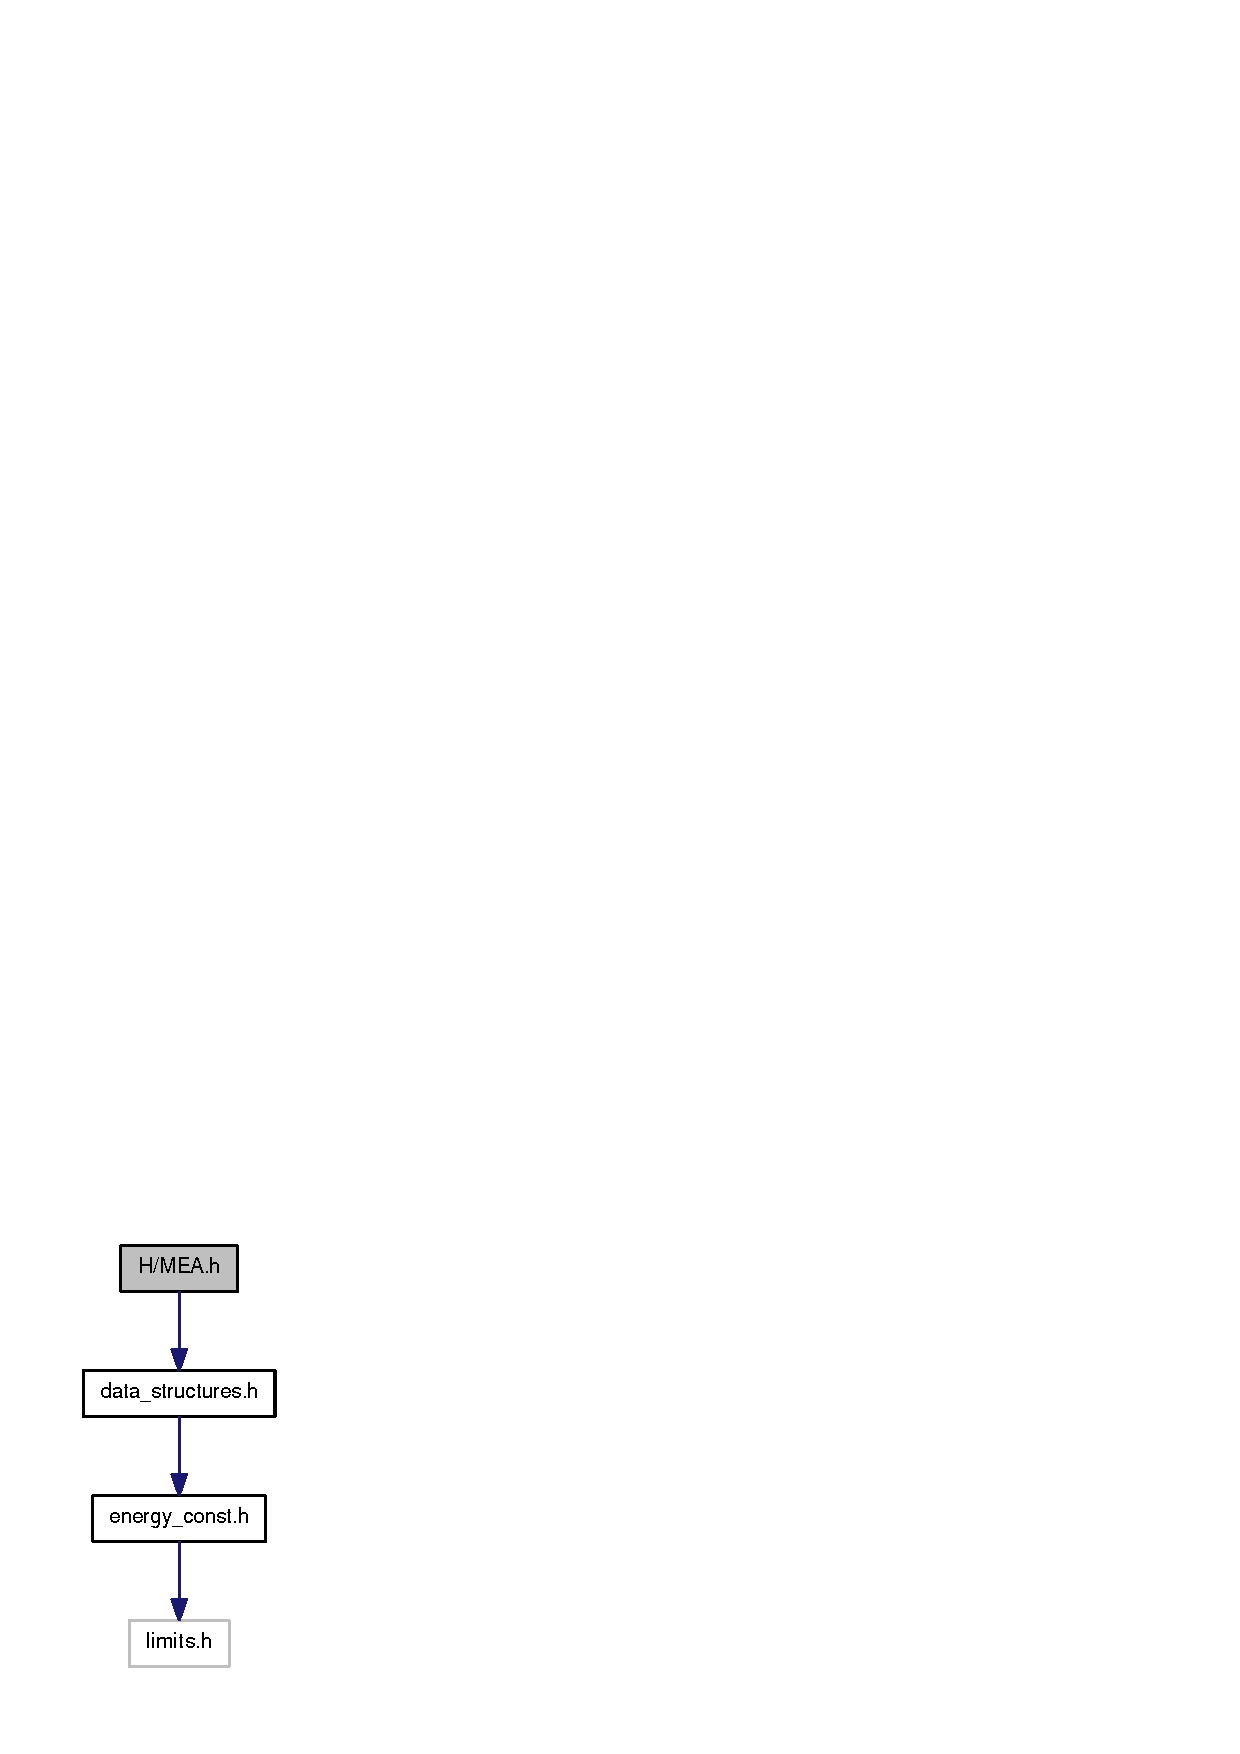
\includegraphics[width=68pt]{MEA_8h__incl}
\end{center}
\end{figure}
\subsection*{Functions}
\begin{DoxyCompactItemize}
\item 
float \hyperlink{MEA_8h_a396ec6144c6a74fcbab4cea6b42d76c3}{MEA} (\hyperlink{structplist}{plist} $\ast$p, char $\ast$structure, double gamma)
\begin{DoxyCompactList}\small\item\em Computes a MEA (maximum expected accuracy) structure. \item\end{DoxyCompactList}\end{DoxyCompactItemize}


\subsection{Detailed Description}
Computes a MEA (maximum expected accuracy) structure. 

\subsection{Function Documentation}
\hypertarget{MEA_8h_a396ec6144c6a74fcbab4cea6b42d76c3}{
\index{MEA.h@{MEA.h}!MEA@{MEA}}
\index{MEA@{MEA}!MEA.h@{MEA.h}}
\subsubsection[{MEA}]{\setlength{\rightskip}{0pt plus 5cm}float MEA ({\bf plist} $\ast$ {\em p}, \/  char $\ast$ {\em structure}, \/  double {\em gamma})}}
\label{MEA_8h_a396ec6144c6a74fcbab4cea6b42d76c3}


Computes a MEA (maximum expected accuracy) structure. 

The algorithm maximizes the expected accuracy \[ A(S) = \sum_{(i,j) \in S} 2 \gamma p_{ij} + \sum_{i \notin S} p^u_i \] Higher values of $\gamma$ result in more base pairs of lower probability and thus higher sensitivity. Low values of $\gamma$ result in structures containing only highly likely pairs (high specificity). The code of the MEA function also demonstrates the use of sparse dynamic programming scheme to reduce the time and memory complexity of folding. 
\hypertarget{mm_8h}{
\section{H/mm.h File Reference}
\label{mm_8h}\index{H/mm.h@{H/mm.h}}
}


Several Maximum Matching implementations.  




\subsection{Detailed Description}
Several Maximum Matching implementations. This file contains the declarations for several maximum matching implementations 
\hypertarget{naview_8h}{
\section{H/naview.h File Reference}
\label{naview_8h}\index{H/naview.h@{H/naview.h}}
}
This graph shows which files directly or indirectly include this file:\nopagebreak
\begin{figure}[H]
\begin{center}
\leavevmode
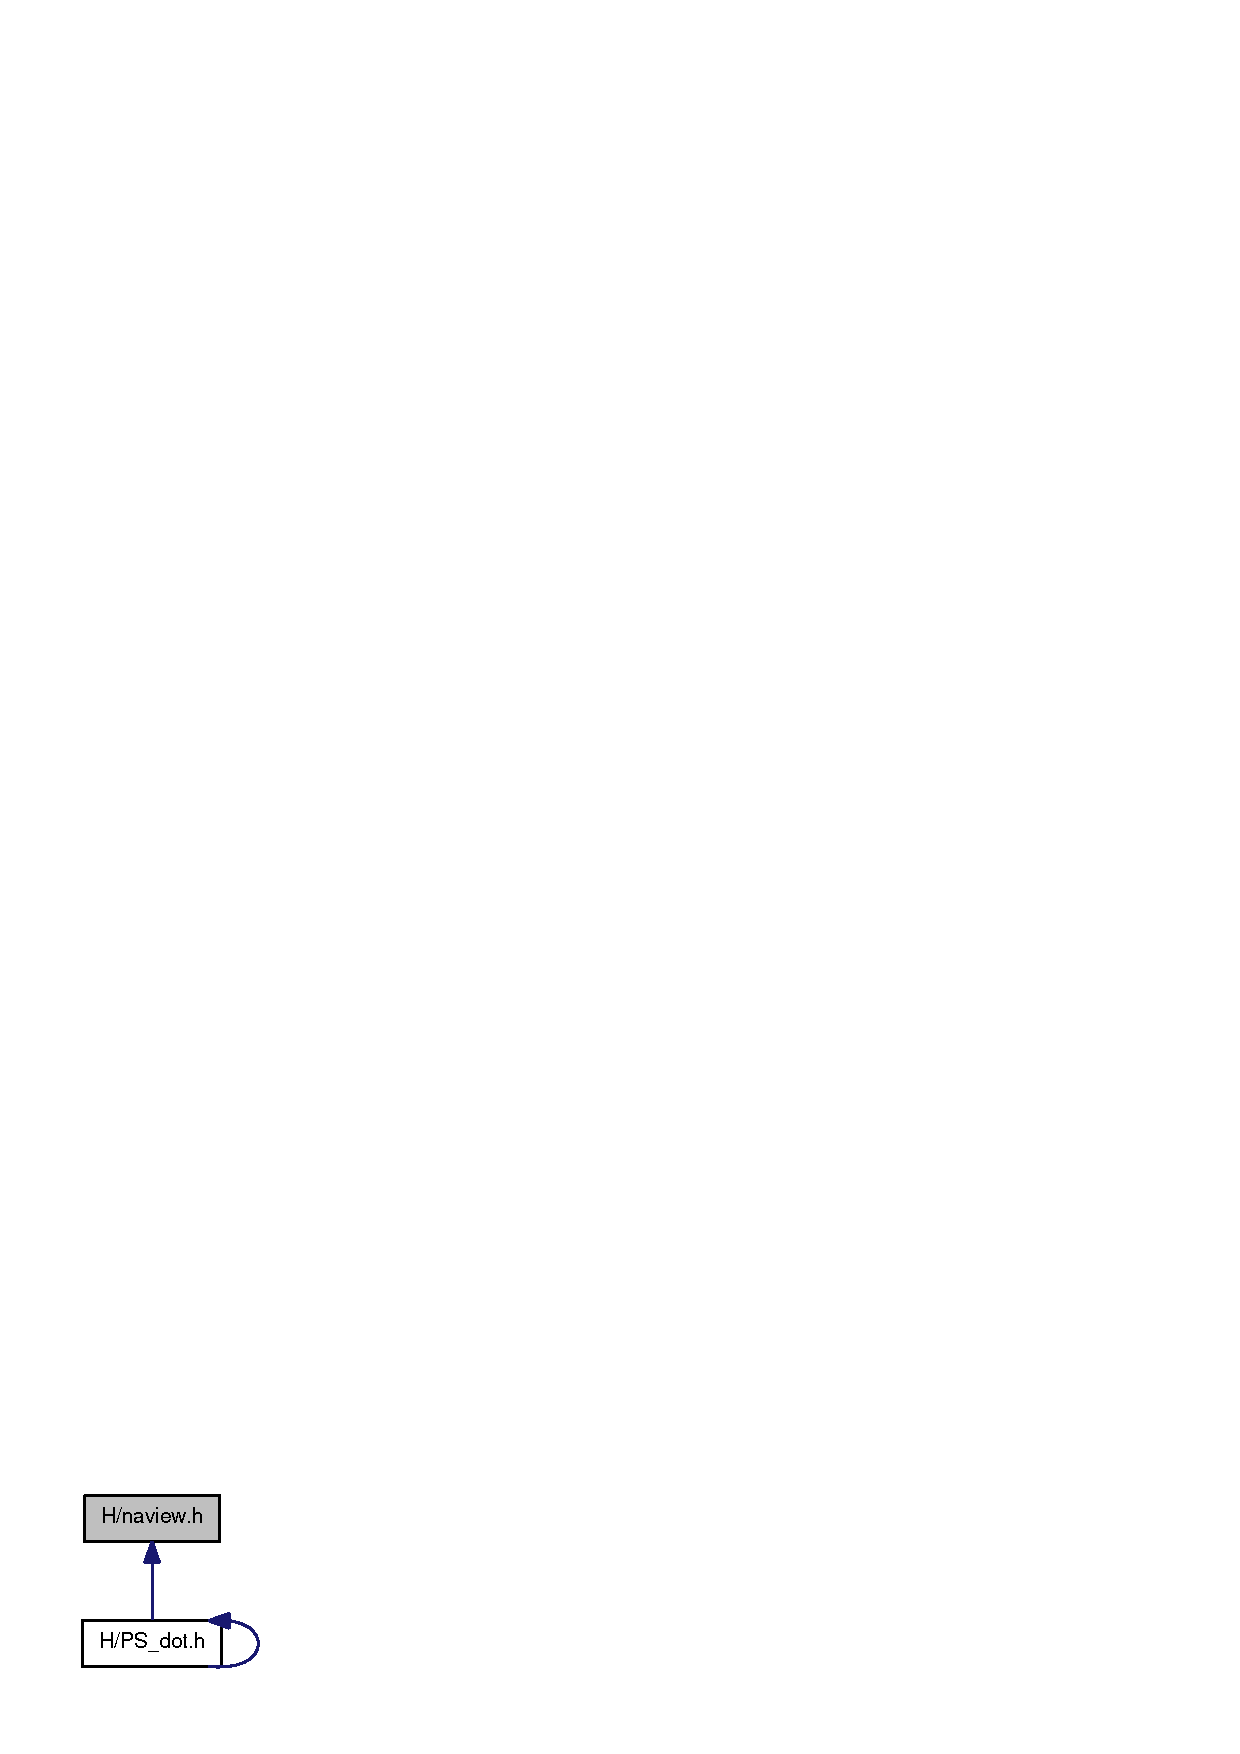
\includegraphics[width=64pt]{naview_8h__dep__incl}
\end{center}
\end{figure}


\subsection{Detailed Description}

\hypertarget{params_8h}{
\section{H/params.h File Reference}
\label{params_8h}\index{H/params.h@{H/params.h}}
}


Several functions to obtain (pre)scaled energy parameter data containers.  


Include dependency graph for params.h:\nopagebreak
\begin{figure}[H]
\begin{center}
\leavevmode
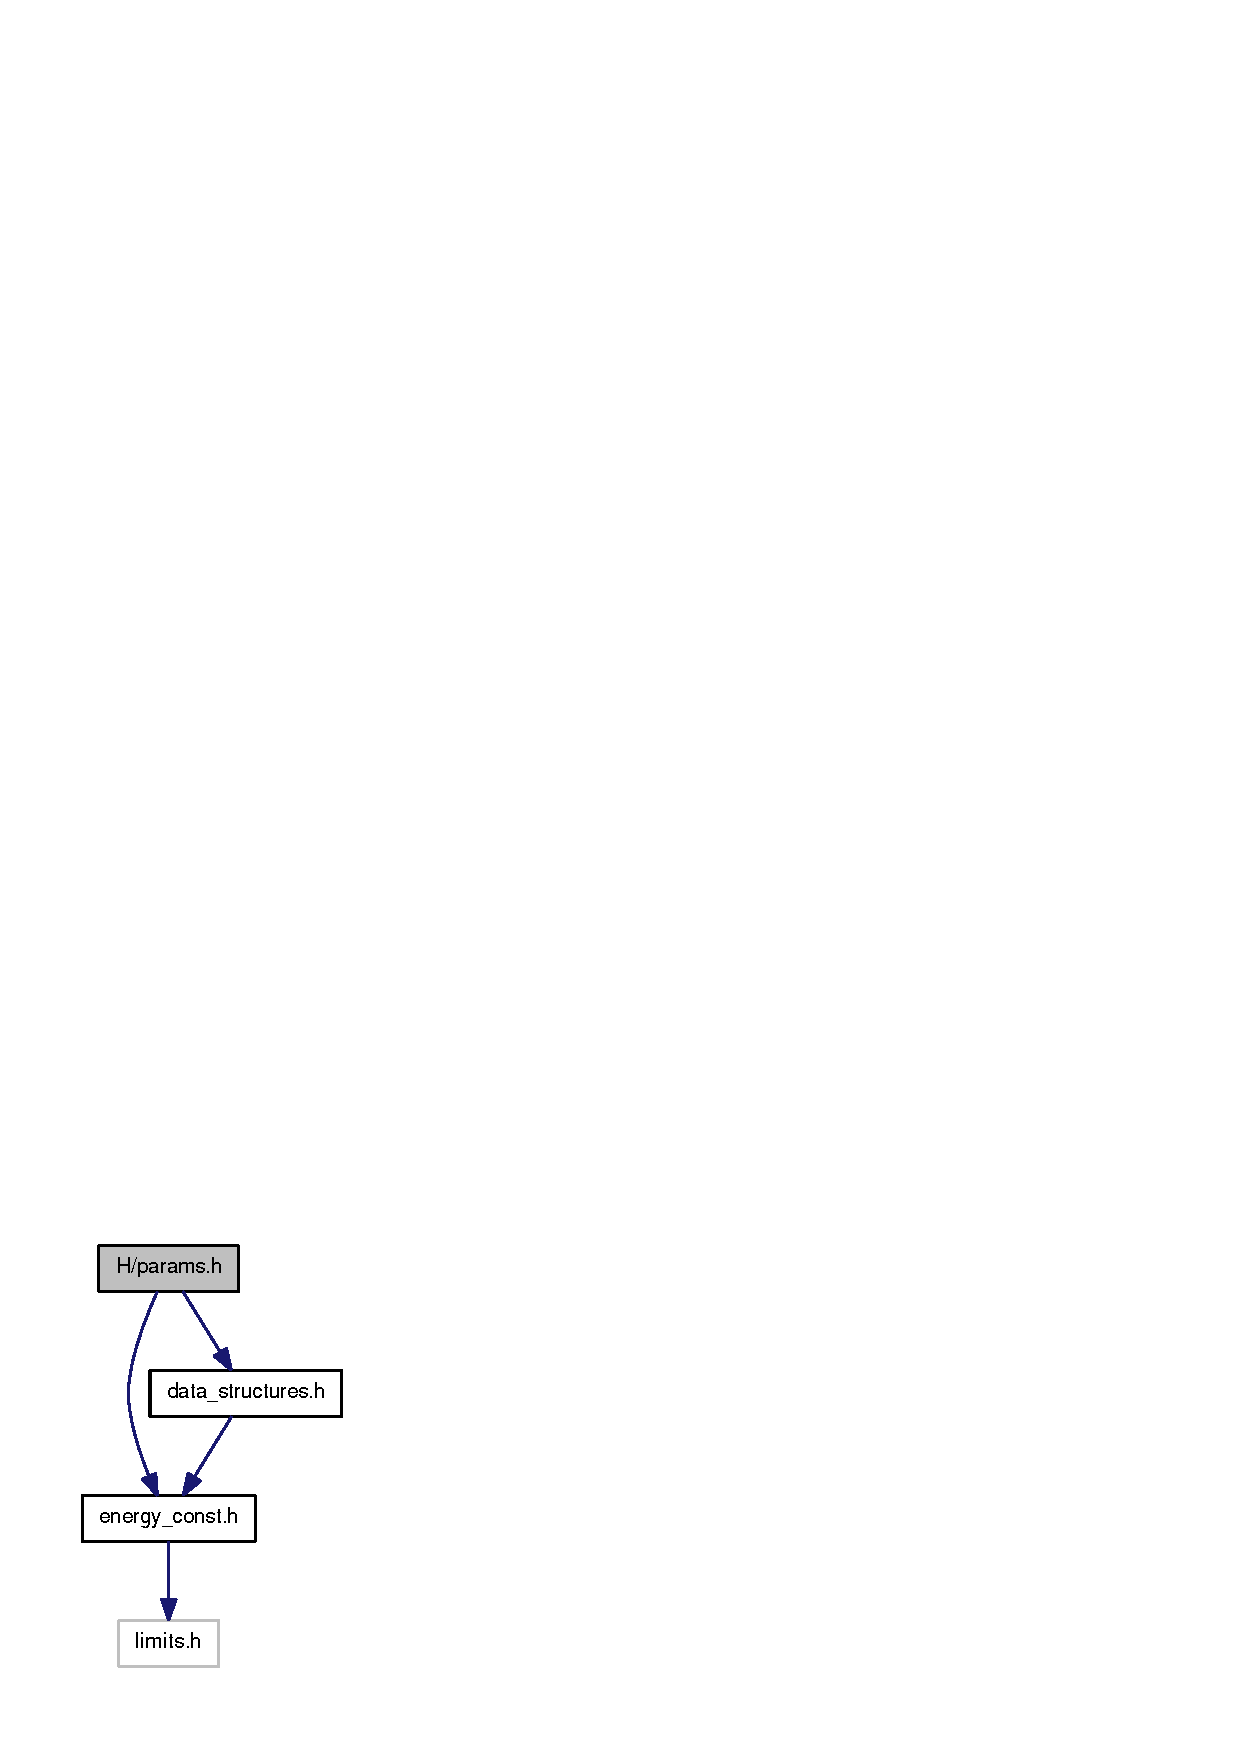
\includegraphics[width=84pt]{params_8h__incl}
\end{center}
\end{figure}
\subsection*{Functions}
\begin{DoxyCompactItemize}
\item 
\hyperlink{structparamT}{paramT} $\ast$ \hyperlink{params_8h_a527ef619cd8210b84d5d53be1e0e29b6}{scale\_\-parameters} (void)
\begin{DoxyCompactList}\small\item\em Get precomputed energy contributions for all the known loop types. \item\end{DoxyCompactList}\item 
\hyperlink{structparamT}{paramT} $\ast$ \hyperlink{params_8h_ac2f3ca440b7eaf4d999fb27da949fe72}{get\_\-scaled\_\-parameters} (double \hyperlink{fold__vars_8h_ab4b11c8d9c758430960896bc3fe82ead}{temperature}, \hyperlink{structmodel__detailsT}{model\_\-detailsT} md)
\begin{DoxyCompactList}\small\item\em Get precomputed energy contributions for all the known loop types. \item\end{DoxyCompactList}\item 
\hyperlink{structpf__paramT}{pf\_\-paramT} $\ast$ \hyperlink{params_8h_ab85f6b6da051f380371deb0d8921bdba}{get\_\-scaled\_\-pf\_\-parameters} (void)
\begin{DoxyCompactList}\small\item\em get a datastructure of type \hyperlink{structpf__paramT}{pf\_\-paramT} which contains the Boltzmann weights of several energy parameters scaled according to the current temperature \item\end{DoxyCompactList}\item 
\hyperlink{structpf__paramT}{pf\_\-paramT} $\ast$ \hyperlink{params_8h_a6fc2f3eef5a3024d44963ac59a42e39d}{get\_\-boltzmann\_\-factors} (double \hyperlink{fold__vars_8h_ab4b11c8d9c758430960896bc3fe82ead}{temperature}, double betaScale, \hyperlink{structmodel__detailsT}{model\_\-detailsT} md, double \hyperlink{fold__vars_8h_ad3b22044065acc6dee0af68931b52cfd}{pf\_\-scale})
\begin{DoxyCompactList}\small\item\em Get precomputed Boltzmann factors of the loop type dependent energy contributions with independent thermodynamic temperature. \item\end{DoxyCompactList}\item 
\hyperlink{structpf__paramT}{pf\_\-paramT} $\ast$ \hyperlink{params_8h_acba212326a051734797e65987260fdd0}{get\_\-boltzmann\_\-factor\_\-copy} (\hyperlink{structpf__paramT}{pf\_\-paramT} $\ast$parameters)
\begin{DoxyCompactList}\small\item\em Get a copy of already precomputed Boltzmann factors. \item\end{DoxyCompactList}\item 
\hyperlink{structpf__paramT}{pf\_\-paramT} $\ast$ \hyperlink{params_8h_aa6a4297a2b91d6f7ae47dd61ca1862a0}{get\_\-scaled\_\-alipf\_\-parameters} (unsigned int n\_\-seq)
\begin{DoxyCompactList}\small\item\em Get precomputed Boltzmann factors of the loop type dependent energy contributions (alifold variant). \item\end{DoxyCompactList}\item 
\hyperlink{structpf__paramT}{pf\_\-paramT} $\ast$ \hyperlink{params_8h_af0c74574b40f2778556535bf9d382828}{get\_\-boltzmann\_\-factors\_\-ali} (unsigned int n\_\-seq, double \hyperlink{fold__vars_8h_ab4b11c8d9c758430960896bc3fe82ead}{temperature}, double betaScale, \hyperlink{structmodel__detailsT}{model\_\-detailsT} md, double \hyperlink{fold__vars_8h_ad3b22044065acc6dee0af68931b52cfd}{pf\_\-scale})
\begin{DoxyCompactList}\small\item\em Get precomputed Boltzmann factors of the loop type dependent energy contributions (alifold variant) with independent thermodynamic temperature. \item\end{DoxyCompactList}\end{DoxyCompactItemize}


\subsection{Detailed Description}
Several functions to obtain (pre)scaled energy parameter data containers. 

\subsection{Function Documentation}
\hypertarget{params_8h_a527ef619cd8210b84d5d53be1e0e29b6}{
\index{params.h@{params.h}!scale\_\-parameters@{scale\_\-parameters}}
\index{scale\_\-parameters@{scale\_\-parameters}!params.h@{params.h}}
\subsubsection[{scale\_\-parameters}]{\setlength{\rightskip}{0pt plus 5cm}{\bf paramT}$\ast$ scale\_\-parameters (void)}}
\label{params_8h_a527ef619cd8210b84d5d53be1e0e29b6}


Get precomputed energy contributions for all the known loop types. 

\begin{DoxyNote}{Note}
OpenMP: This function relies on several global model settings variables and thus is not to be considered threadsafe. See \hyperlink{params_8h_ac2f3ca440b7eaf4d999fb27da949fe72}{get\_\-scaled\_\-parameters()} for a completely threadsafe implementation.
\end{DoxyNote}
\begin{DoxyReturn}{Returns}
A set of precomputed energy contributions 
\end{DoxyReturn}
\hypertarget{params_8h_ac2f3ca440b7eaf4d999fb27da949fe72}{
\index{params.h@{params.h}!get\_\-scaled\_\-parameters@{get\_\-scaled\_\-parameters}}
\index{get\_\-scaled\_\-parameters@{get\_\-scaled\_\-parameters}!params.h@{params.h}}
\subsubsection[{get\_\-scaled\_\-parameters}]{\setlength{\rightskip}{0pt plus 5cm}{\bf paramT}$\ast$ get\_\-scaled\_\-parameters (double {\em temperature}, \/  {\bf model\_\-detailsT} {\em md})}}
\label{params_8h_ac2f3ca440b7eaf4d999fb27da949fe72}


Get precomputed energy contributions for all the known loop types. 

Call this function to retrieve precomputed energy contributions, i.e. scaled according to the temperature passed. Furthermore, this function assumes a data structure that contains the model details as well, such that subsequent folding recursions are able to retrieve the correct model settings

\begin{DoxySeeAlso}{See also}
\hyperlink{structmodel__detailsT}{model\_\-detailsT}, \hyperlink{fold__vars_8h_a4c3257186a796182462f18a5480ac8b3}{set\_\-model\_\-details()}
\end{DoxySeeAlso}

\begin{DoxyParams}{Parameters}
\item[{\em temperature}]The temperature in degrees Celcius 
\begin{DoxyParams}{Parameters}
\item[{\em md}]The model details \begin{DoxyReturn}{Returns}
precomputed energy contributions and model settings 
\end{DoxyReturn}
\end{DoxyParams}
\end{DoxyParams}
\hypertarget{params_8h_ab85f6b6da051f380371deb0d8921bdba}{
\index{params.h@{params.h}!get\_\-scaled\_\-pf\_\-parameters@{get\_\-scaled\_\-pf\_\-parameters}}
\index{get\_\-scaled\_\-pf\_\-parameters@{get\_\-scaled\_\-pf\_\-parameters}!params.h@{params.h}}
\subsubsection[{get\_\-scaled\_\-pf\_\-parameters}]{\setlength{\rightskip}{0pt plus 5cm}{\bf pf\_\-paramT}$\ast$ get\_\-scaled\_\-pf\_\-parameters (void)}}
\label{params_8h_ab85f6b6da051f380371deb0d8921bdba}


get a datastructure of type \hyperlink{structpf__paramT}{pf\_\-paramT} which contains the Boltzmann weights of several energy parameters scaled according to the current temperature 

\begin{DoxyReturn}{Returns}
The datastructure containing Boltzmann weights for use in partition function calculations 
\end{DoxyReturn}
\hypertarget{params_8h_a6fc2f3eef5a3024d44963ac59a42e39d}{
\index{params.h@{params.h}!get\_\-boltzmann\_\-factors@{get\_\-boltzmann\_\-factors}}
\index{get\_\-boltzmann\_\-factors@{get\_\-boltzmann\_\-factors}!params.h@{params.h}}
\subsubsection[{get\_\-boltzmann\_\-factors}]{\setlength{\rightskip}{0pt plus 5cm}{\bf pf\_\-paramT}$\ast$ get\_\-boltzmann\_\-factors (double {\em temperature}, \/  double {\em betaScale}, \/  {\bf model\_\-detailsT} {\em md}, \/  double {\em pf\_\-scale})}}
\label{params_8h_a6fc2f3eef5a3024d44963ac59a42e39d}


Get precomputed Boltzmann factors of the loop type dependent energy contributions with independent thermodynamic temperature. 

This function returns a data structure that contains all necessary precalculated Boltzmann factors for each loop type contribution.\par
 In contrast to \hyperlink{params_8h_ab85f6b6da051f380371deb0d8921bdba}{get\_\-scaled\_\-pf\_\-parameters()}, this function enables setting of independent temperatures for both, the individual energy contributions as well as the thermodynamic temperature used in $ exp(-\Delta G / kT) $

\begin{DoxySeeAlso}{See also}
\hyperlink{params_8h_ab85f6b6da051f380371deb0d8921bdba}{get\_\-scaled\_\-pf\_\-parameters()}, \hyperlink{params_8h_acba212326a051734797e65987260fdd0}{get\_\-boltzmann\_\-factor\_\-copy()}
\end{DoxySeeAlso}

\begin{DoxyParams}{Parameters}
\item[{\em dangle\_\-model}]The dangle model to be used (possible values: 0 or 2) 
\begin{DoxyParams}{Parameters}
\item[{\em temperature}]The temperature in degC used for (re-\/)scaling the energy contributions 
\begin{DoxyParams}{Parameters}
\item[{\em alpha}]A scaling value that is used as a multiplication factor for the absolute temperature of the system \begin{DoxyReturn}{Returns}
A set of precomputed Boltzmann factors 
\end{DoxyReturn}
\end{DoxyParams}
\end{DoxyParams}
\end{DoxyParams}
\hypertarget{params_8h_acba212326a051734797e65987260fdd0}{
\index{params.h@{params.h}!get\_\-boltzmann\_\-factor\_\-copy@{get\_\-boltzmann\_\-factor\_\-copy}}
\index{get\_\-boltzmann\_\-factor\_\-copy@{get\_\-boltzmann\_\-factor\_\-copy}!params.h@{params.h}}
\subsubsection[{get\_\-boltzmann\_\-factor\_\-copy}]{\setlength{\rightskip}{0pt plus 5cm}{\bf pf\_\-paramT}$\ast$ get\_\-boltzmann\_\-factor\_\-copy ({\bf pf\_\-paramT} $\ast$ {\em parameters})}}
\label{params_8h_acba212326a051734797e65987260fdd0}


Get a copy of already precomputed Boltzmann factors. 

\begin{DoxySeeAlso}{See also}
\hyperlink{params_8h_a6fc2f3eef5a3024d44963ac59a42e39d}{get\_\-boltzmann\_\-factors()}, \hyperlink{params_8h_ab85f6b6da051f380371deb0d8921bdba}{get\_\-scaled\_\-pf\_\-parameters()}
\end{DoxySeeAlso}

\begin{DoxyParams}{Parameters}
\item[{\em parameters}]The input data structure that shall be copied \begin{DoxyReturn}{Returns}
A copy of the provided Boltzmann factor dataset 
\end{DoxyReturn}
\end{DoxyParams}
\hypertarget{params_8h_aa6a4297a2b91d6f7ae47dd61ca1862a0}{
\index{params.h@{params.h}!get\_\-scaled\_\-alipf\_\-parameters@{get\_\-scaled\_\-alipf\_\-parameters}}
\index{get\_\-scaled\_\-alipf\_\-parameters@{get\_\-scaled\_\-alipf\_\-parameters}!params.h@{params.h}}
\subsubsection[{get\_\-scaled\_\-alipf\_\-parameters}]{\setlength{\rightskip}{0pt plus 5cm}{\bf pf\_\-paramT}$\ast$ get\_\-scaled\_\-alipf\_\-parameters (unsigned int {\em n\_\-seq})}}
\label{params_8h_aa6a4297a2b91d6f7ae47dd61ca1862a0}


Get precomputed Boltzmann factors of the loop type dependent energy contributions (alifold variant). 

\hypertarget{params_8h_af0c74574b40f2778556535bf9d382828}{
\index{params.h@{params.h}!get\_\-boltzmann\_\-factors\_\-ali@{get\_\-boltzmann\_\-factors\_\-ali}}
\index{get\_\-boltzmann\_\-factors\_\-ali@{get\_\-boltzmann\_\-factors\_\-ali}!params.h@{params.h}}
\subsubsection[{get\_\-boltzmann\_\-factors\_\-ali}]{\setlength{\rightskip}{0pt plus 5cm}{\bf pf\_\-paramT}$\ast$ get\_\-boltzmann\_\-factors\_\-ali (unsigned int {\em n\_\-seq}, \/  double {\em temperature}, \/  double {\em betaScale}, \/  {\bf model\_\-detailsT} {\em md}, \/  double {\em pf\_\-scale})}}
\label{params_8h_af0c74574b40f2778556535bf9d382828}


Get precomputed Boltzmann factors of the loop type dependent energy contributions (alifold variant) with independent thermodynamic temperature. 


\hypertarget{part__func_8h}{
\section{H/part\_\-func.h File Reference}
\label{part__func_8h}\index{H/part\_\-func.h@{H/part\_\-func.h}}
}


Partition function of single RNA sequences.  


Include dependency graph for part\_\-func.h:\nopagebreak
\begin{figure}[H]
\begin{center}
\leavevmode
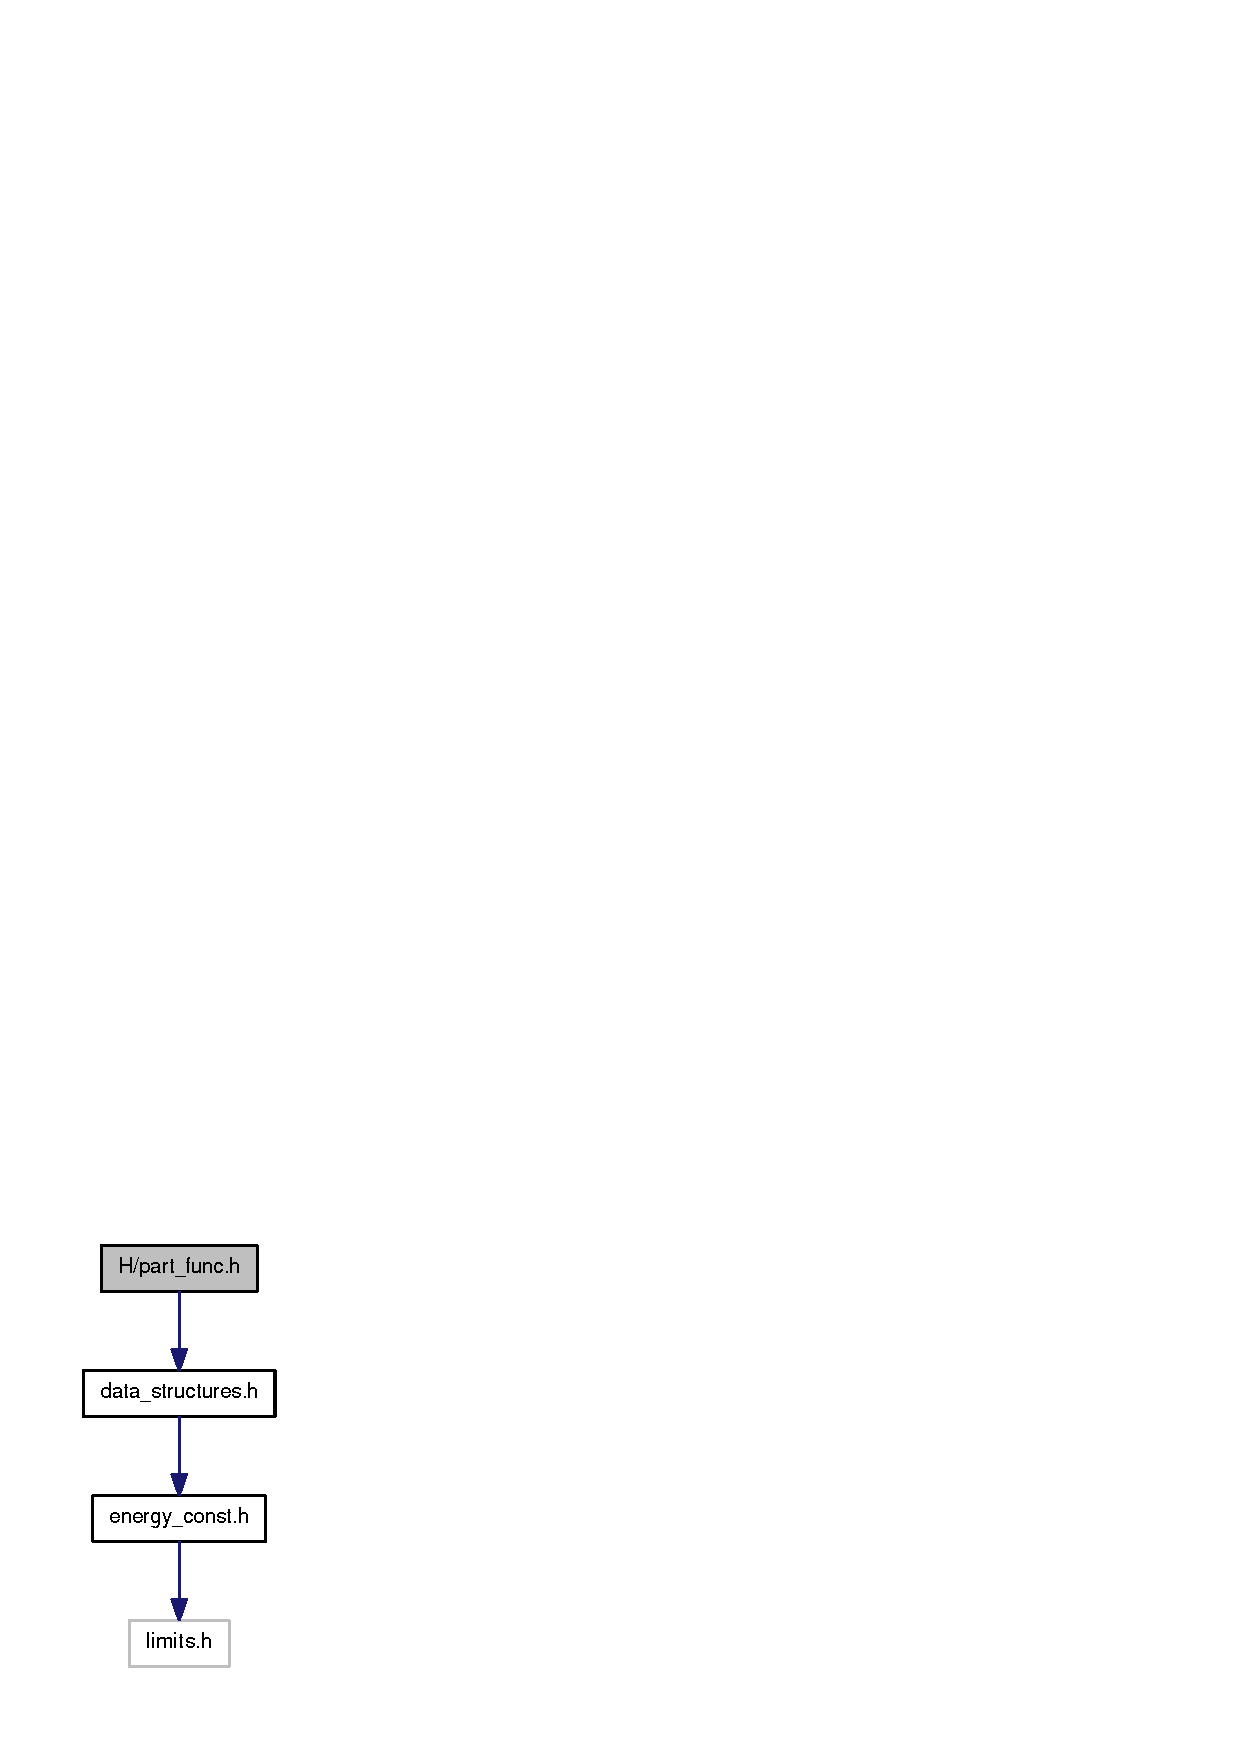
\includegraphics[width=68pt]{part__func_8h__incl}
\end{center}
\end{figure}
\subsection*{Functions}
\begin{DoxyCompactItemize}
\item 
float \hyperlink{part__func_8h_a1839c61275760944b3a007c41d5c0823}{pf\_\-fold\_\-par} (const char $\ast$sequence, char $\ast$structure, \hyperlink{structpf__paramT}{pf\_\-paramT} $\ast$parameters, int calculate\_\-bppm, int is\_\-constrained, int is\_\-circular)
\begin{DoxyCompactList}\small\item\em Compute the partition function $Q$ for a given RNA sequence. \item\end{DoxyCompactList}\item 
float \hyperlink{part__func_8h_adc3db3d98742427e7001a7fd36ef28c2}{pf\_\-fold} (const char $\ast$sequence, char $\ast$structure)
\begin{DoxyCompactList}\small\item\em Compute the partition function $Q$ of an RNA sequence. \item\end{DoxyCompactList}\item 
float \hyperlink{part__func_8h_a819ce5fca8984004ac81c4a3b04cb735}{pf\_\-circ\_\-fold} (const char $\ast$sequence, char $\ast$structure)
\begin{DoxyCompactList}\small\item\em Compute the partition function of a circular RNA sequence. \item\end{DoxyCompactList}\item 
char $\ast$ \hyperlink{part__func_8h_ac03ca6db186bb3bf0a2a326d7fb3ba03}{pbacktrack} (char $\ast$sequence)
\begin{DoxyCompactList}\small\item\em Sample a secondary structure from the Boltzmann ensemble according its probability\par
. \item\end{DoxyCompactList}\item 
char $\ast$ \hyperlink{part__func_8h_a00474051204ac9ad576b3e45174d03ff}{pbacktrack\_\-circ} (char $\ast$sequence)
\begin{DoxyCompactList}\small\item\em Sample a secondary structure of a circular RNA from the Boltzmann ensemble according its probability. \item\end{DoxyCompactList}\item 
void \hyperlink{part__func_8h_ae73db3f49a94f0f72e067ecd12681dbd}{free\_\-pf\_\-arrays} (void)
\begin{DoxyCompactList}\small\item\em Free arrays for the partition function recursions. \item\end{DoxyCompactList}\item 
void \hyperlink{part__func_8h_a384e927890f9c034ff09fa66da102d28}{update\_\-pf\_\-params} (int length)
\begin{DoxyCompactList}\small\item\em Recalculate energy parameters. \item\end{DoxyCompactList}\item 
FLT\_\-OR\_\-DBL $\ast$ \hyperlink{part__func_8h_ac5ac7ee281aae1c5cc5898a841178073}{export\_\-bppm} (void)
\begin{DoxyCompactList}\small\item\em Get a pointer to the base pair probability array. \item\end{DoxyCompactList}\item 
void \hyperlink{part__func_8h_a2f29542659beb5ebd176631a3da11580}{assign\_\-plist\_\-from\_\-pr} (\hyperlink{structplist}{plist} $\ast$$\ast$pl, FLT\_\-OR\_\-DBL $\ast$probs, int length, double cutoff)
\begin{DoxyCompactList}\small\item\em Create a plist from a probability matrix. \item\end{DoxyCompactList}\item 
int \hyperlink{part__func_8h_a42faebdfce6f070c5f89adfc8427525c}{get\_\-pf\_\-arrays} (short $\ast$$\ast$S\_\-p, short $\ast$$\ast$S1\_\-p, char $\ast$$\ast$ptype\_\-p, FLT\_\-OR\_\-DBL $\ast$$\ast$qb\_\-p, FLT\_\-OR\_\-DBL $\ast$$\ast$qm\_\-p, FLT\_\-OR\_\-DBL $\ast$$\ast$q1k\_\-p, FLT\_\-OR\_\-DBL $\ast$$\ast$qln\_\-p)
\begin{DoxyCompactList}\small\item\em Get the pointers to (almost) all relavant computation arrays used in partition function computation. \item\end{DoxyCompactList}\item 
\hypertarget{part__func_8h_a189e2a1ec6cc32c53ea72f7543b0441e}{
double \hyperlink{part__func_8h_a189e2a1ec6cc32c53ea72f7543b0441e}{get\_\-subseq\_\-F} (int i, int j)}
\label{part__func_8h_a189e2a1ec6cc32c53ea72f7543b0441e}

\begin{DoxyCompactList}\small\item\em Get the free energy of a subsequence from the q\mbox{[}\mbox{]} array. \item\end{DoxyCompactList}\item 
char $\ast$ \hyperlink{part__func_8h_a9aba0ba1433a6d259331e0fe9fc4a9a6}{get\_\-centroid\_\-struct\_\-pl} (int length, double $\ast$dist, \hyperlink{structplist}{plist} $\ast$pl)
\begin{DoxyCompactList}\small\item\em Get the centroid structure of the ensemble. \item\end{DoxyCompactList}\item 
char $\ast$ \hyperlink{part__func_8h_ac92486ce514677256f4a832dc518759c}{get\_\-centroid\_\-struct\_\-pr} (int length, double $\ast$dist, FLT\_\-OR\_\-DBL $\ast$\hyperlink{fold__vars_8h_ac98ec419070aee6831b44e5c700f090f}{pr})
\begin{DoxyCompactList}\small\item\em Get the centroid structure of the ensemble. \item\end{DoxyCompactList}\item 
double \hyperlink{part__func_8h_a79cbc375af65f11609feb6b055269e7d}{mean\_\-bp\_\-distance} (int length)
\begin{DoxyCompactList}\small\item\em Get the mean base pair distance of the last partition function computation. \item\end{DoxyCompactList}\item 
double \hyperlink{part__func_8h_ad5ba36cef8d01cf4244cc09b9bf1ce1d}{mean\_\-bp\_\-distance\_\-pr} (int length, FLT\_\-OR\_\-DBL $\ast$\hyperlink{fold__vars_8h_ac98ec419070aee6831b44e5c700f090f}{pr})
\begin{DoxyCompactList}\small\item\em Get the mean base pair distance in the thermodynamic ensemble. \item\end{DoxyCompactList}\item 
\hypertarget{part__func_8h_a129d81c4a1ead793c5b2311333e03dfa}{
void \hyperlink{part__func_8h_a129d81c4a1ead793c5b2311333e03dfa}{bppm\_\-to\_\-structure} (char $\ast$structure, FLT\_\-OR\_\-DBL $\ast$\hyperlink{fold__vars_8h_ac98ec419070aee6831b44e5c700f090f}{pr}, unsigned int length)}
\label{part__func_8h_a129d81c4a1ead793c5b2311333e03dfa}

\begin{DoxyCompactList}\small\item\em Create a dot-\/bracket like structure string from base pair probability matrix. \item\end{DoxyCompactList}\item 
\hypertarget{part__func_8h_a49962ad6242b8c628de6ca16bb831c1d}{
char \hyperlink{part__func_8h_a49962ad6242b8c628de6ca16bb831c1d}{bppm\_\-symbol} (const float $\ast$x)}
\label{part__func_8h_a49962ad6242b8c628de6ca16bb831c1d}

\begin{DoxyCompactList}\small\item\em Get a pseudo dot bracket notation for a given probability information. \item\end{DoxyCompactList}\item 
void \hyperlink{part__func_8h_a15176e23eceeff8c7d14eabcfec8a2af}{init\_\-pf\_\-fold} (int length)
\begin{DoxyCompactList}\small\item\em Allocate space for \hyperlink{part__func_8h_adc3db3d98742427e7001a7fd36ef28c2}{pf\_\-fold()}. \item\end{DoxyCompactList}\item 
char $\ast$ \hyperlink{part__func_8h_ae89a63bd83e75a80b2ba36d20b31ce81}{centroid} (int length, double $\ast$dist)
\item 
double \hyperlink{part__func_8h_ae9556ba7ded44fe2321b6f67c3fc02a3}{mean\_\-bp\_\-dist} (int length)
\begin{DoxyCompactList}\small\item\em get the mean pair distance of ensemble \item\end{DoxyCompactList}\item 
double \hyperlink{part__func_8h_a68ba6f3a48e08ca131ab54621ce3a2d7}{expLoopEnergy} (int u1, int u2, int type, int type2, short si1, short sj1, short sp1, short sq1)
\item 
double \hyperlink{part__func_8h_a7b6ab474cc80accc48010ccfcc59f96b}{expHairpinEnergy} (int u, int type, short si1, short sj1, const char $\ast$string)
\end{DoxyCompactItemize}
\subsection*{Variables}
\begin{DoxyCompactItemize}
\item 
\hypertarget{part__func_8h_acd79b1a570e6ad9be24cb11fe8cae30a}{
int \hyperlink{part__func_8h_acd79b1a570e6ad9be24cb11fe8cae30a}{st\_\-back}}
\label{part__func_8h_acd79b1a570e6ad9be24cb11fe8cae30a}

\begin{DoxyCompactList}\small\item\em a flag indicating that auxilary arrays are needed throughout the computations which are necessary for stochastic backtracking \item\end{DoxyCompactList}\end{DoxyCompactItemize}


\subsection{Detailed Description}
Partition function of single RNA sequences. This file includes (almost) all function declarations within the {\bfseries RNAlib} that are related to Partion function folding...

\begin{DoxyNote}{Note}
If you plan on using the functions provided from this section of the RNAlib concurrently via {\bfseries OpenMP} you have to place a {\itshape COPYIN\/} clause right before your {\itshape PARALLEL\/} directive! Otherwise, some functions may not behave as expected. A complete list of variables that have to be passed to the {\itshape COPYIN\/} clause can be found in the detailed description of each function below. 
\end{DoxyNote}


\subsection{Function Documentation}
\hypertarget{part__func_8h_a1839c61275760944b3a007c41d5c0823}{
\index{part\_\-func.h@{part\_\-func.h}!pf\_\-fold\_\-par@{pf\_\-fold\_\-par}}
\index{pf\_\-fold\_\-par@{pf\_\-fold\_\-par}!part_func.h@{part\_\-func.h}}
\subsubsection[{pf\_\-fold\_\-par}]{\setlength{\rightskip}{0pt plus 5cm}float pf\_\-fold\_\-par (const char $\ast$ {\em sequence}, \/  char $\ast$ {\em structure}, \/  {\bf pf\_\-paramT} $\ast$ {\em parameters}, \/  int {\em calculate\_\-bppm}, \/  int {\em is\_\-constrained}, \/  int {\em is\_\-circular})}}
\label{part__func_8h_a1839c61275760944b3a007c41d5c0823}


Compute the partition function $Q$ for a given RNA sequence. 

If {\itshape structure\/} is not a NULL pointer on input, it contains on return a string consisting of the letters \char`\"{} . , $|$ \{ \} ( ) \char`\"{} denoting bases that are essentially unpaired, weakly paired, strongly paired without preference, weakly upstream (downstream) paired, or strongly up-\/ (down-\/)stream paired bases, respectively. If \hyperlink{fold__vars_8h_a0afc287c2464866d94858c39175154af}{fold\_\-constrained} is not 0, the {\itshape structure\/} string is interpreted on input as a list of constraints for the folding. The character \char`\"{}x\char`\"{} marks bases that must be unpaired, matching brackets \char`\"{} ( ) \char`\"{} denote base pairs, all other characters are ignored. Any pairs conflicting with the constraint will be forbidden. This is usually sufficient to ensure the constraints are honored. If tha parameter calculate\_\-bppm is set to 0 base pairing probabilities will not be computed (saving CPU time), otherwise after calculations took place \hyperlink{fold__vars_8h_ac98ec419070aee6831b44e5c700f090f}{pr} will contain the probability that bases {\itshape i\/} and {\itshape j\/} pair. \begin{DoxyNote}{Note}
The global array \hyperlink{fold__vars_8h_ac98ec419070aee6831b44e5c700f090f}{pr} is deprecated and the user who wants the calculated base pair probabilities for further computations is advised to use the function \hyperlink{part__func_8h_ac5ac7ee281aae1c5cc5898a841178073}{export\_\-bppm()}
\end{DoxyNote}
\begin{DoxySeeAlso}{See also}
\hyperlink{part__func_8h_a819ce5fca8984004ac81c4a3b04cb735}{pf\_\-circ\_\-fold()}, \hyperlink{part__func_8h_a129d81c4a1ead793c5b2311333e03dfa}{bppm\_\-to\_\-structure()}, \hyperlink{part__func_8h_ac5ac7ee281aae1c5cc5898a841178073}{export\_\-bppm()}, \hyperlink{params_8h_a6fc2f3eef5a3024d44963ac59a42e39d}{get\_\-boltzmann\_\-factors()}
\end{DoxySeeAlso}

\begin{DoxyParams}{Parameters}
\item[{\em sequence}]The RNA sequence input 
\begin{DoxyParams}{Parameters}
\item[{\em structure}]A pointer to a char array where a base pair probability information can be stored in a pseudo-\/dot-\/bracket notation (may be NULL, too) 
\begin{DoxyParams}{Parameters}
\item[{\em parameters}]Data structure containing the precalculated Boltzmann factors 
\begin{DoxyParams}{Parameters}
\item[{\em calculate\_\-bppm}]Switch to Base pair probability calculations on/off (0==off) 
\begin{DoxyParams}{Parameters}
\item[{\em is\_\-constrained}]Switch to indicate that a structure contraint is passed via the structure argument (0==off) 
\begin{DoxyParams}{Parameters}
\item[{\em is\_\-circular}]Switch to (de-\/)activate postprocessing steps in case RNA sequence is circular (0==off) \begin{DoxyReturn}{Returns}
The Gibbs free energy of the ensemble ($G = -RT \cdot \log(Q) $) in kcal/mol 
\end{DoxyReturn}
\end{DoxyParams}
\end{DoxyParams}
\end{DoxyParams}
\end{DoxyParams}
\end{DoxyParams}
\end{DoxyParams}
\hypertarget{part__func_8h_adc3db3d98742427e7001a7fd36ef28c2}{
\index{part\_\-func.h@{part\_\-func.h}!pf\_\-fold@{pf\_\-fold}}
\index{pf\_\-fold@{pf\_\-fold}!part_func.h@{part\_\-func.h}}
\subsubsection[{pf\_\-fold}]{\setlength{\rightskip}{0pt plus 5cm}float pf\_\-fold (const char $\ast$ {\em sequence}, \/  char $\ast$ {\em structure})}}
\label{part__func_8h_adc3db3d98742427e7001a7fd36ef28c2}


Compute the partition function $Q$ of an RNA sequence. 

If {\itshape structure\/} is not a NULL pointer on input, it contains on return a string consisting of the letters \char`\"{} . , $|$ \{ \} ( ) \char`\"{} denoting bases that are essentially unpaired, weakly paired, strongly paired without preference, weakly upstream (downstream) paired, or strongly up-\/ (down-\/)stream paired bases, respectively. If \hyperlink{fold__vars_8h_a0afc287c2464866d94858c39175154af}{fold\_\-constrained} is not 0, the {\itshape structure\/} string is interpreted on input as a list of constraints for the folding. The character \char`\"{}x\char`\"{} marks bases that must be unpaired, matching brackets \char`\"{} ( ) \char`\"{} denote base pairs, all other characters are ignored. Any pairs conflicting with the constraint will be forbidden. This is usually sufficient to ensure the constraints are honored. If \hyperlink{fold__vars_8h_ad512b5dd4dbec60faccfe137bb474489}{do\_\-backtrack} has been set to 0 base pairing probabilities will not be computed (saving CPU time), otherwise \hyperlink{fold__vars_8h_ac98ec419070aee6831b44e5c700f090f}{pr} will contain the probability that bases {\itshape i\/} and {\itshape j\/} pair. \begin{DoxyNote}{Note}
The global array \hyperlink{fold__vars_8h_ac98ec419070aee6831b44e5c700f090f}{pr} is deprecated and the user who wants the calculated base pair probabilities for further computations is advised to use the function \hyperlink{part__func_8h_ac5ac7ee281aae1c5cc5898a841178073}{export\_\-bppm()}
\end{DoxyNote}
\begin{DoxySeeAlso}{See also}
\hyperlink{part__func_8h_a819ce5fca8984004ac81c4a3b04cb735}{pf\_\-circ\_\-fold()}, \hyperlink{part__func_8h_a129d81c4a1ead793c5b2311333e03dfa}{bppm\_\-to\_\-structure()}, \hyperlink{part__func_8h_ac5ac7ee281aae1c5cc5898a841178073}{export\_\-bppm()}
\end{DoxySeeAlso}

\begin{DoxyParams}{Parameters}
\item[{\em sequence}]The RNA sequence input 
\begin{DoxyParams}{Parameters}
\item[{\em structure}]A pointer to a char array where a base pair probability information can be stored in a pseudo-\/dot-\/bracket notation (may be NULL, too) \begin{DoxyReturn}{Returns}
The Gibbs free energy of the ensemble ($G = -RT \cdot \log(Q) $) in kcal/mol 
\end{DoxyReturn}
\end{DoxyParams}
\end{DoxyParams}
\hypertarget{part__func_8h_a819ce5fca8984004ac81c4a3b04cb735}{
\index{part\_\-func.h@{part\_\-func.h}!pf\_\-circ\_\-fold@{pf\_\-circ\_\-fold}}
\index{pf\_\-circ\_\-fold@{pf\_\-circ\_\-fold}!part_func.h@{part\_\-func.h}}
\subsubsection[{pf\_\-circ\_\-fold}]{\setlength{\rightskip}{0pt plus 5cm}float pf\_\-circ\_\-fold (const char $\ast$ {\em sequence}, \/  char $\ast$ {\em structure})}}
\label{part__func_8h_a819ce5fca8984004ac81c4a3b04cb735}


Compute the partition function of a circular RNA sequence. 

\begin{DoxySeeAlso}{See also}
\hyperlink{part__func_8h_adc3db3d98742427e7001a7fd36ef28c2}{pf\_\-fold()}, \hyperlink{part__func_8h_a1839c61275760944b3a007c41d5c0823}{pf\_\-fold\_\-par()}
\end{DoxySeeAlso}

\begin{DoxyParams}{Parameters}
\item[{\em sequence}]The RNA sequence input 
\begin{DoxyParams}{Parameters}
\item[{\em structure}]A pointer to a char array where a base pair probability information can be stored in a pseudo-\/dot-\/bracket notation (may be NULL, too) \begin{DoxyReturn}{Returns}
The Gibbs free energy of the ensemble ($G = -RT \cdot \log(Q) $) in kcal/mol 
\end{DoxyReturn}
\end{DoxyParams}
\end{DoxyParams}
\hypertarget{part__func_8h_ac03ca6db186bb3bf0a2a326d7fb3ba03}{
\index{part\_\-func.h@{part\_\-func.h}!pbacktrack@{pbacktrack}}
\index{pbacktrack@{pbacktrack}!part_func.h@{part\_\-func.h}}
\subsubsection[{pbacktrack}]{\setlength{\rightskip}{0pt plus 5cm}char$\ast$ pbacktrack (char $\ast$ {\em sequence})}}
\label{part__func_8h_ac03ca6db186bb3bf0a2a326d7fb3ba03}


Sample a secondary structure from the Boltzmann ensemble according its probability\par
. 

\begin{DoxyNote}{Note}
You have to call \hyperlink{part__func_8h_adc3db3d98742427e7001a7fd36ef28c2}{pf\_\-fold()} first in order to fill the partition function matrices

{\bfseries OpenMP notice:}\par
This function relies on passing the following variables to the appropriate {\itshape COPYIN\/} clause {\itshape (additionally to the ones needed by \hyperlink{part__func_8h_adc3db3d98742427e7001a7fd36ef28c2}{pf\_\-fold()})\/}:\par
 pstruc, sequence
\end{DoxyNote}

\begin{DoxyParams}{Parameters}
\item[{\em sequence}]The RNA sequence \begin{DoxyReturn}{Returns}
A sampled secondary structure in dot-\/bracket notation 
\end{DoxyReturn}
\end{DoxyParams}
\hypertarget{part__func_8h_a00474051204ac9ad576b3e45174d03ff}{
\index{part\_\-func.h@{part\_\-func.h}!pbacktrack\_\-circ@{pbacktrack\_\-circ}}
\index{pbacktrack\_\-circ@{pbacktrack\_\-circ}!part_func.h@{part\_\-func.h}}
\subsubsection[{pbacktrack\_\-circ}]{\setlength{\rightskip}{0pt plus 5cm}char$\ast$ pbacktrack\_\-circ (char $\ast$ {\em sequence})}}
\label{part__func_8h_a00474051204ac9ad576b3e45174d03ff}


Sample a secondary structure of a circular RNA from the Boltzmann ensemble according its probability. 

This function does the same as \hyperlink{part__func_8h_ac03ca6db186bb3bf0a2a326d7fb3ba03}{pbacktrack()} but assumes the RNA molecule to be circular

\begin{DoxyNote}{Note}
{\bfseries OpenMP notice:}\par
This function relies on passing the following variables to the appropriate {\itshape COPYIN\/} clause {\itshape (additionally to the ones needed by \hyperlink{part__func_8h_adc3db3d98742427e7001a7fd36ef28c2}{pf\_\-fold()})\/}:\par
 pstruc, sequence
\end{DoxyNote}

\begin{DoxyParams}{Parameters}
\item[{\em sequence}]The RNA sequence \begin{DoxyReturn}{Returns}
A sampled secondary structure in dot-\/bracket notation 
\end{DoxyReturn}
\end{DoxyParams}
\hypertarget{part__func_8h_ae73db3f49a94f0f72e067ecd12681dbd}{
\index{part\_\-func.h@{part\_\-func.h}!free\_\-pf\_\-arrays@{free\_\-pf\_\-arrays}}
\index{free\_\-pf\_\-arrays@{free\_\-pf\_\-arrays}!part_func.h@{part\_\-func.h}}
\subsubsection[{free\_\-pf\_\-arrays}]{\setlength{\rightskip}{0pt plus 5cm}void free\_\-pf\_\-arrays (void)}}
\label{part__func_8h_ae73db3f49a94f0f72e067ecd12681dbd}


Free arrays for the partition function recursions. 

Call this function if you want to free all allocated memory associated with the partition function forward recursion. \begin{DoxyNote}{Note}
Successive calls of \hyperlink{part__func_8h_adc3db3d98742427e7001a7fd36ef28c2}{pf\_\-fold()}, \hyperlink{part__func_8h_a819ce5fca8984004ac81c4a3b04cb735}{pf\_\-circ\_\-fold()} already check if they should free any memory from a previous run. 

{\bfseries OpenMP notice:}\par
 This function should be called before leaving a thread in order to avoid leaking memory
\end{DoxyNote}
\begin{DoxySeeAlso}{See also}
\hyperlink{part__func_8h_adc3db3d98742427e7001a7fd36ef28c2}{pf\_\-fold()}, \hyperlink{part__func_8h_a819ce5fca8984004ac81c4a3b04cb735}{pf\_\-circ\_\-fold()} 
\end{DoxySeeAlso}
\hypertarget{part__func_8h_a384e927890f9c034ff09fa66da102d28}{
\index{part\_\-func.h@{part\_\-func.h}!update\_\-pf\_\-params@{update\_\-pf\_\-params}}
\index{update\_\-pf\_\-params@{update\_\-pf\_\-params}!part_func.h@{part\_\-func.h}}
\subsubsection[{update\_\-pf\_\-params}]{\setlength{\rightskip}{0pt plus 5cm}void update\_\-pf\_\-params (int {\em length})}}
\label{part__func_8h_a384e927890f9c034ff09fa66da102d28}


Recalculate energy parameters. 

Call this function to recalculate the pair matrix and energy parameters after a change in folding parameters like \hyperlink{fold__vars_8h_ab4b11c8d9c758430960896bc3fe82ead}{temperature} \hypertarget{part__func_8h_ac5ac7ee281aae1c5cc5898a841178073}{
\index{part\_\-func.h@{part\_\-func.h}!export\_\-bppm@{export\_\-bppm}}
\index{export\_\-bppm@{export\_\-bppm}!part_func.h@{part\_\-func.h}}
\subsubsection[{export\_\-bppm}]{\setlength{\rightskip}{0pt plus 5cm}FLT\_\-OR\_\-DBL$\ast$ export\_\-bppm (void)}}
\label{part__func_8h_ac5ac7ee281aae1c5cc5898a841178073}


Get a pointer to the base pair probability array. 

Accessing the base pair probabilities for a pair (i,j) is achieved by \begin{DoxyVerb}FLT_OR_DBL *pr = export_bppm(); pr_ij = pr[iindx[i]-j]; \end{DoxyVerb}


\begin{DoxyNote}{Note}
Call \hyperlink{part__func_8h_adc3db3d98742427e7001a7fd36ef28c2}{pf\_\-fold()} before using this function!
\end{DoxyNote}
\begin{DoxySeeAlso}{See also}
\hyperlink{part__func_8h_adc3db3d98742427e7001a7fd36ef28c2}{pf\_\-fold()}, \hyperlink{part__func_8h_a819ce5fca8984004ac81c4a3b04cb735}{pf\_\-circ\_\-fold()}, \hyperlink{utils_8h_a55c0f6b3b07b6adf2ee235ba901fe397}{get\_\-iindx()}
\end{DoxySeeAlso}
\begin{DoxyReturn}{Returns}
A pointer to the base pair probability array 
\end{DoxyReturn}
\hypertarget{part__func_8h_a2f29542659beb5ebd176631a3da11580}{
\index{part\_\-func.h@{part\_\-func.h}!assign\_\-plist\_\-from\_\-pr@{assign\_\-plist\_\-from\_\-pr}}
\index{assign\_\-plist\_\-from\_\-pr@{assign\_\-plist\_\-from\_\-pr}!part_func.h@{part\_\-func.h}}
\subsubsection[{assign\_\-plist\_\-from\_\-pr}]{\setlength{\rightskip}{0pt plus 5cm}void assign\_\-plist\_\-from\_\-pr ({\bf plist} $\ast$$\ast$ {\em pl}, \/  FLT\_\-OR\_\-DBL $\ast$ {\em probs}, \/  int {\em length}, \/  double {\em cutoff})}}
\label{part__func_8h_a2f29542659beb5ebd176631a3da11580}


Create a plist from a probability matrix. 

The probability matrix given is parsed and all pair probabilities above the given threshold are used to create an entry in the plist

The end of the plist is marked by sequence positions i as well as j equal to 0. This condition should be used to stop looping over its entries

\begin{DoxyNote}{Note}
This function is threadsafe
\end{DoxyNote}

\begin{DoxyParams}{Parameters}
\item[{\em pl}]A pointer to the plist that is to be created 
\begin{DoxyParams}{Parameters}
\item[{\em probs}]The probability matrix used for creting the plist 
\begin{DoxyParams}{Parameters}
\item[{\em length}]The length of the RNA sequence 
\begin{DoxyParams}{Parameters}
\item[{\em cutoff}]The cutoff value \end{DoxyParams}
\end{DoxyParams}
\end{DoxyParams}
\end{DoxyParams}
\hypertarget{part__func_8h_a42faebdfce6f070c5f89adfc8427525c}{
\index{part\_\-func.h@{part\_\-func.h}!get\_\-pf\_\-arrays@{get\_\-pf\_\-arrays}}
\index{get\_\-pf\_\-arrays@{get\_\-pf\_\-arrays}!part_func.h@{part\_\-func.h}}
\subsubsection[{get\_\-pf\_\-arrays}]{\setlength{\rightskip}{0pt plus 5cm}int get\_\-pf\_\-arrays (short $\ast$$\ast$ {\em S\_\-p}, \/  short $\ast$$\ast$ {\em S1\_\-p}, \/  char $\ast$$\ast$ {\em ptype\_\-p}, \/  FLT\_\-OR\_\-DBL $\ast$$\ast$ {\em qb\_\-p}, \/  FLT\_\-OR\_\-DBL $\ast$$\ast$ {\em qm\_\-p}, \/  FLT\_\-OR\_\-DBL $\ast$$\ast$ {\em q1k\_\-p}, \/  FLT\_\-OR\_\-DBL $\ast$$\ast$ {\em qln\_\-p})}}
\label{part__func_8h_a42faebdfce6f070c5f89adfc8427525c}


Get the pointers to (almost) all relavant computation arrays used in partition function computation. 

\begin{DoxyNote}{Note}
In order to assign meaningful pointers, you have to call pf\_\-fold first!
\end{DoxyNote}
\begin{DoxySeeAlso}{See also}
\hyperlink{part__func_8h_adc3db3d98742427e7001a7fd36ef28c2}{pf\_\-fold()}, \hyperlink{part__func_8h_a819ce5fca8984004ac81c4a3b04cb735}{pf\_\-circ\_\-fold()}
\end{DoxySeeAlso}

\begin{DoxyParams}{Parameters}
\item[{\em S\_\-p}]A pointer to the 'S' array (integer representation of nucleotides) 
\begin{DoxyParams}{Parameters}
\item[{\em S1\_\-p}]A pointer to the 'S1' array (2nd integer representation of nucleotides) 
\begin{DoxyParams}{Parameters}
\item[{\em ptype\_\-p}]A pointer to the pair type matrix 
\begin{DoxyParams}{Parameters}
\item[{\em qb\_\-p}]A pointer to the Q$^{\mbox{B}}$  matrix 
\begin{DoxyParams}{Parameters}
\item[{\em qm\_\-p}]A pointer to the Q$^{\mbox{M}}$  matrix 
\begin{DoxyParams}{Parameters}
\item[{\em q1k\_\-p}]A pointer to the 5' slice of the Q matrix ($q1k(k) = Q(1, k)$) 
\begin{DoxyParams}{Parameters}
\item[{\em qln\_\-p}]A pointer to the 3' slice of the Q matrix ($qln(l) = Q(l, n)$) \begin{DoxyReturn}{Returns}
Non Zero if everything went fine, 0 otherwise 
\end{DoxyReturn}
\end{DoxyParams}
\end{DoxyParams}
\end{DoxyParams}
\end{DoxyParams}
\end{DoxyParams}
\end{DoxyParams}
\end{DoxyParams}
\hypertarget{part__func_8h_a9aba0ba1433a6d259331e0fe9fc4a9a6}{
\index{part\_\-func.h@{part\_\-func.h}!get\_\-centroid\_\-struct\_\-pl@{get\_\-centroid\_\-struct\_\-pl}}
\index{get\_\-centroid\_\-struct\_\-pl@{get\_\-centroid\_\-struct\_\-pl}!part_func.h@{part\_\-func.h}}
\subsubsection[{get\_\-centroid\_\-struct\_\-pl}]{\setlength{\rightskip}{0pt plus 5cm}char$\ast$ get\_\-centroid\_\-struct\_\-pl (int {\em length}, \/  double $\ast$ {\em dist}, \/  {\bf plist} $\ast$ {\em pl})}}
\label{part__func_8h_a9aba0ba1433a6d259331e0fe9fc4a9a6}


Get the centroid structure of the ensemble. 

This function is a threadsafe replacement for \hyperlink{part__func_8h_ae89a63bd83e75a80b2ba36d20b31ce81}{centroid()} with a 'plist' input

The centroid is the structure with the minimal average distance to all other structures \par
 $ <d(S)> = \sum_{(i,j) \in S} (1-p_{ij}) + \sum_{(i,j) \notin S} p_{ij} $ \par
 Thus, the centroid is simply the structure containing all pairs with $p_ij>0.5$ The distance of the centroid to the ensemble is written to the memory adressed by {\itshape dist\/}.


\begin{DoxyParams}{Parameters}
\item[{\em length}]The length of the sequence 
\begin{DoxyParams}{Parameters}
\item[{\em dist}]A pointer to the distance variable where the centroid distance will be written to 
\begin{DoxyParams}{Parameters}
\item[{\em pl}]A pair list containing base pair probability information about the ensemble \begin{DoxyReturn}{Returns}
The centroid structure of the ensemble in dot-\/bracket notation 
\end{DoxyReturn}
\end{DoxyParams}
\end{DoxyParams}
\end{DoxyParams}
\hypertarget{part__func_8h_ac92486ce514677256f4a832dc518759c}{
\index{part\_\-func.h@{part\_\-func.h}!get\_\-centroid\_\-struct\_\-pr@{get\_\-centroid\_\-struct\_\-pr}}
\index{get\_\-centroid\_\-struct\_\-pr@{get\_\-centroid\_\-struct\_\-pr}!part_func.h@{part\_\-func.h}}
\subsubsection[{get\_\-centroid\_\-struct\_\-pr}]{\setlength{\rightskip}{0pt plus 5cm}char$\ast$ get\_\-centroid\_\-struct\_\-pr (int {\em length}, \/  double $\ast$ {\em dist}, \/  FLT\_\-OR\_\-DBL $\ast$ {\em pr})}}
\label{part__func_8h_ac92486ce514677256f4a832dc518759c}


Get the centroid structure of the ensemble. 

This function is a threadsafe replacement for \hyperlink{part__func_8h_ae89a63bd83e75a80b2ba36d20b31ce81}{centroid()} with a probability array input

The centroid is the structure with the minimal average distance to all other structures \par
 $ <d(S)> = \sum_{(i,j) \in S} (1-p_{ij}) + \sum_{(i,j) \notin S} p_{ij} $ \par
 Thus, the centroid is simply the structure containing all pairs with $p_ij>0.5$ The distance of the centroid to the ensemble is written to the memory adressed by {\itshape dist\/}.


\begin{DoxyParams}{Parameters}
\item[{\em length}]The length of the sequence 
\begin{DoxyParams}{Parameters}
\item[{\em dist}]A pointer to the distance variable where the centroid distance will be written to 
\begin{DoxyParams}{Parameters}
\item[{\em pr}]A upper triangular matrix containing base pair probabilities (access via iindx \hyperlink{utils_8h_a55c0f6b3b07b6adf2ee235ba901fe397}{get\_\-iindx()} ) \begin{DoxyReturn}{Returns}
The centroid structure of the ensemble in dot-\/bracket notation 
\end{DoxyReturn}
\end{DoxyParams}
\end{DoxyParams}
\end{DoxyParams}
\hypertarget{part__func_8h_a79cbc375af65f11609feb6b055269e7d}{
\index{part\_\-func.h@{part\_\-func.h}!mean\_\-bp\_\-distance@{mean\_\-bp\_\-distance}}
\index{mean\_\-bp\_\-distance@{mean\_\-bp\_\-distance}!part_func.h@{part\_\-func.h}}
\subsubsection[{mean\_\-bp\_\-distance}]{\setlength{\rightskip}{0pt plus 5cm}double mean\_\-bp\_\-distance (int {\em length})}}
\label{part__func_8h_a79cbc375af65f11609feb6b055269e7d}


Get the mean base pair distance of the last partition function computation. 

\begin{DoxyNote}{Note}
To ensure thread-\/safety, use the function \hyperlink{part__func_8h_ad5ba36cef8d01cf4244cc09b9bf1ce1d}{mean\_\-bp\_\-distance\_\-pr()} instead!
\end{DoxyNote}
\begin{DoxySeeAlso}{See also}
\hyperlink{part__func_8h_ad5ba36cef8d01cf4244cc09b9bf1ce1d}{mean\_\-bp\_\-distance\_\-pr()}
\end{DoxySeeAlso}

\begin{DoxyParams}{Parameters}
\item[{\em length}]\begin{DoxyReturn}{Returns}
mean base pair distance in thermodynamic ensemble 
\end{DoxyReturn}
\end{DoxyParams}
\hypertarget{part__func_8h_ad5ba36cef8d01cf4244cc09b9bf1ce1d}{
\index{part\_\-func.h@{part\_\-func.h}!mean\_\-bp\_\-distance\_\-pr@{mean\_\-bp\_\-distance\_\-pr}}
\index{mean\_\-bp\_\-distance\_\-pr@{mean\_\-bp\_\-distance\_\-pr}!part_func.h@{part\_\-func.h}}
\subsubsection[{mean\_\-bp\_\-distance\_\-pr}]{\setlength{\rightskip}{0pt plus 5cm}double mean\_\-bp\_\-distance\_\-pr (int {\em length}, \/  FLT\_\-OR\_\-DBL $\ast$ {\em pr})}}
\label{part__func_8h_ad5ba36cef8d01cf4244cc09b9bf1ce1d}


Get the mean base pair distance in the thermodynamic ensemble. 

This is a threadsafe implementation of \hyperlink{part__func_8h_ae9556ba7ded44fe2321b6f67c3fc02a3}{mean\_\-bp\_\-dist()} !

$<d> = \sum_{a,b} p_a p_b d(S_a,S_b)$\par
 this can be computed from the pair probs $p_ij$ as\par
 $<d> = \sum_{ij} p_{ij}(1-p_{ij})$

\begin{DoxyNote}{Note}
This function is threadsafe
\end{DoxyNote}

\begin{DoxyParams}{Parameters}
\item[{\em length}]The length of the sequence 
\begin{DoxyParams}{Parameters}
\item[{\em pr}]The matrix containing the base pair probabilities \begin{DoxyReturn}{Returns}
The mean pair distance of the structure ensemble 
\end{DoxyReturn}
\end{DoxyParams}
\end{DoxyParams}
\hypertarget{part__func_8h_a15176e23eceeff8c7d14eabcfec8a2af}{
\index{part\_\-func.h@{part\_\-func.h}!init\_\-pf\_\-fold@{init\_\-pf\_\-fold}}
\index{init\_\-pf\_\-fold@{init\_\-pf\_\-fold}!part_func.h@{part\_\-func.h}}
\subsubsection[{init\_\-pf\_\-fold}]{\setlength{\rightskip}{0pt plus 5cm}void init\_\-pf\_\-fold (int {\em length})}}
\label{part__func_8h_a15176e23eceeff8c7d14eabcfec8a2af}


Allocate space for \hyperlink{part__func_8h_adc3db3d98742427e7001a7fd36ef28c2}{pf\_\-fold()}. 

\begin{Desc}
\item[\hyperlink{deprecated__deprecated000011}{Deprecated}]This function is obsolete and will be removed soon! \end{Desc}
\hypertarget{part__func_8h_ae89a63bd83e75a80b2ba36d20b31ce81}{
\index{part\_\-func.h@{part\_\-func.h}!centroid@{centroid}}
\index{centroid@{centroid}!part_func.h@{part\_\-func.h}}
\subsubsection[{centroid}]{\setlength{\rightskip}{0pt plus 5cm}char$\ast$ centroid (int {\em length}, \/  double $\ast$ {\em dist})}}
\label{part__func_8h_ae89a63bd83e75a80b2ba36d20b31ce81}
\begin{Desc}
\item[\hyperlink{deprecated__deprecated000012}{Deprecated}]This function is deprecated and should not be used anymore as it is not threadsafe! \end{Desc}
\begin{DoxySeeAlso}{See also}
\hyperlink{part__func_8h_a9aba0ba1433a6d259331e0fe9fc4a9a6}{get\_\-centroid\_\-struct\_\-pl()}, \hyperlink{part__func_8h_ac92486ce514677256f4a832dc518759c}{get\_\-centroid\_\-struct\_\-pr()} 
\end{DoxySeeAlso}
\hypertarget{part__func_8h_ae9556ba7ded44fe2321b6f67c3fc02a3}{
\index{part\_\-func.h@{part\_\-func.h}!mean\_\-bp\_\-dist@{mean\_\-bp\_\-dist}}
\index{mean\_\-bp\_\-dist@{mean\_\-bp\_\-dist}!part_func.h@{part\_\-func.h}}
\subsubsection[{mean\_\-bp\_\-dist}]{\setlength{\rightskip}{0pt plus 5cm}double mean\_\-bp\_\-dist (int {\em length})}}
\label{part__func_8h_ae9556ba7ded44fe2321b6f67c3fc02a3}


get the mean pair distance of ensemble 

\begin{Desc}
\item[\hyperlink{deprecated__deprecated000013}{Deprecated}]This function is not threadsafe and should not be used anymore. Use \hyperlink{part__func_8h_a79cbc375af65f11609feb6b055269e7d}{mean\_\-bp\_\-distance()} instead! \end{Desc}
\hypertarget{part__func_8h_a68ba6f3a48e08ca131ab54621ce3a2d7}{
\index{part\_\-func.h@{part\_\-func.h}!expLoopEnergy@{expLoopEnergy}}
\index{expLoopEnergy@{expLoopEnergy}!part_func.h@{part\_\-func.h}}
\subsubsection[{expLoopEnergy}]{\setlength{\rightskip}{0pt plus 5cm}double expLoopEnergy (int {\em u1}, \/  int {\em u2}, \/  int {\em type}, \/  int {\em type2}, \/  short {\em si1}, \/  short {\em sj1}, \/  short {\em sp1}, \/  short {\em sq1})}}
\label{part__func_8h_a68ba6f3a48e08ca131ab54621ce3a2d7}
\begin{Desc}
\item[\hyperlink{deprecated__deprecated000014}{Deprecated}]Use \hyperlink{loop__energies_8h_aa5e98e524e2a41e290b942b09544bc9e}{exp\_\-E\_\-IntLoop()} from \hyperlink{loop__energies_8h}{loop\_\-energies.h} instead \end{Desc}
\hypertarget{part__func_8h_a7b6ab474cc80accc48010ccfcc59f96b}{
\index{part\_\-func.h@{part\_\-func.h}!expHairpinEnergy@{expHairpinEnergy}}
\index{expHairpinEnergy@{expHairpinEnergy}!part_func.h@{part\_\-func.h}}
\subsubsection[{expHairpinEnergy}]{\setlength{\rightskip}{0pt plus 5cm}double expHairpinEnergy (int {\em u}, \/  int {\em type}, \/  short {\em si1}, \/  short {\em sj1}, \/  const char $\ast$ {\em string})}}
\label{part__func_8h_a7b6ab474cc80accc48010ccfcc59f96b}
\begin{Desc}
\item[\hyperlink{deprecated__deprecated000015}{Deprecated}]Use \hyperlink{loop__energies_8h_a0e128184bb097dc2da33706f33b555a6}{exp\_\-E\_\-Hairpin()} from \hyperlink{loop__energies_8h}{loop\_\-energies.h} instead \end{Desc}

\hypertarget{part__func__co_8h}{
\section{H/part\_\-func\_\-co.h File Reference}
\label{part__func__co_8h}\index{H/part\_\-func\_\-co.h@{H/part\_\-func\_\-co.h}}
}


Partition function for two RNA sequences.  


Include dependency graph for part\_\-func\_\-co.h:\nopagebreak
\begin{figure}[H]
\begin{center}
\leavevmode
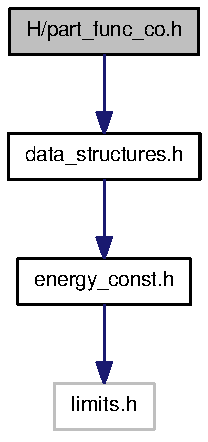
\includegraphics[width=68pt]{part__func__co_8h__incl}
\end{center}
\end{figure}
\subsection*{Functions}
\begin{DoxyCompactItemize}
\item 
\hyperlink{structcofoldF}{cofoldF} \hyperlink{part__func__co_8h_aa86a5f998789ed71813d23d7307a791b}{co\_\-pf\_\-fold} (char $\ast$sequence, char $\ast$structure)
\begin{DoxyCompactList}\small\item\em Calculate partition function and base pair probabilities. \item\end{DoxyCompactList}\item 
\hyperlink{structcofoldF}{cofoldF} \hyperlink{part__func__co_8h_abd873b450832ab5f21101fc5ab354d21}{co\_\-pf\_\-fold\_\-par} (char $\ast$sequence, char $\ast$structure, \hyperlink{structpf__paramT}{pf\_\-paramT} $\ast$parameters, int calculate\_\-bppm, int is\_\-constrained)
\begin{DoxyCompactList}\small\item\em Calculate partition function and base pair probabilities. \item\end{DoxyCompactList}\item 
FLT\_\-OR\_\-DBL $\ast$ \hyperlink{part__func__co_8h_ad94c0133157bed6912fe7fe866e0039e}{export\_\-co\_\-bppm} (void)
\begin{DoxyCompactList}\small\item\em Get a pointer to the base pair probability array. \item\end{DoxyCompactList}\item 
\hypertarget{part__func__co_8h_ade3ce34ae8214811374b1d28a40dc247}{
void \hyperlink{part__func__co_8h_ade3ce34ae8214811374b1d28a40dc247}{free\_\-co\_\-pf\_\-arrays} (void)}
\label{part__func__co_8h_ade3ce34ae8214811374b1d28a40dc247}

\begin{DoxyCompactList}\small\item\em Free the memory occupied by \hyperlink{part__func__co_8h_aa86a5f998789ed71813d23d7307a791b}{co\_\-pf\_\-fold()}. \item\end{DoxyCompactList}\item 
void \hyperlink{part__func__co_8h_a6e0f36c1f9b7d9dd4bfbad914c1119e5}{update\_\-co\_\-pf\_\-params} (int length)
\begin{DoxyCompactList}\small\item\em Recalculate energy parameters. \item\end{DoxyCompactList}\item 
void \hyperlink{part__func__co_8h_a117d880df45bef444d5e2785ffa40a53}{update\_\-co\_\-pf\_\-params\_\-par} (int length, \hyperlink{structpf__paramT}{pf\_\-paramT} $\ast$parameters)
\begin{DoxyCompactList}\small\item\em Recalculate energy parameters. \item\end{DoxyCompactList}\item 
void \hyperlink{part__func__co_8h_a15ae04ac5ab84e876dcf0093120cb617}{compute\_\-probabilities} (double FAB, double FEA, double FEB, struct \hyperlink{structplist}{plist} $\ast$prAB, struct \hyperlink{structplist}{plist} $\ast$prA, struct \hyperlink{structplist}{plist} $\ast$prB, int Alength)
\begin{DoxyCompactList}\small\item\em Compute Boltzmann probabilities of dimerization without homodimers. \item\end{DoxyCompactList}\item 
\hyperlink{structConcEnt}{ConcEnt} $\ast$ \hyperlink{part__func__co_8h_a5545cb936ac4ff93c7d699d46e72e8c7}{get\_\-concentrations} (double FEAB, double FEAA, double FEBB, double FEA, double FEB, double $\ast$startconc)
\begin{DoxyCompactList}\small\item\em Given two start monomer concentrations a and b, compute the concentrations in thermodynamic equilibrium of all dimers and the monomers. \item\end{DoxyCompactList}\item 
\hyperlink{structplist}{plist} $\ast$ \hyperlink{part__func__co_8h_a334de3c96e2186abfbdc0eaea6d08b14}{get\_\-plist} (struct \hyperlink{structplist}{plist} $\ast$pl, int length, double cut\_\-off)
\begin{DoxyCompactList}\small\item\em DO NOT USE THIS FUNCTION ANYMORE. \item\end{DoxyCompactList}\item 
void \hyperlink{part__func__co_8h_aa12dda9dd6179cdd22bcce87c0682c07}{init\_\-co\_\-pf\_\-fold} (int length)
\begin{DoxyCompactList}\small\item\em DO NOT USE THIS FUNCTION ANYMORE. \item\end{DoxyCompactList}\end{DoxyCompactItemize}
\subsection*{Variables}
\begin{DoxyCompactItemize}
\item 
\hypertarget{part__func__co_8h_aff27888c4088cc1f60fd59cbd589474c}{
int \hyperlink{part__func__co_8h_aff27888c4088cc1f60fd59cbd589474c}{mirnatog}}
\label{part__func__co_8h_aff27888c4088cc1f60fd59cbd589474c}

\begin{DoxyCompactList}\small\item\em Toggles no intrabp in 2nd mol. \item\end{DoxyCompactList}\item 
\hypertarget{part__func__co_8h_ac2d1851a710a8561390861155ca988fe}{
double \hyperlink{part__func__co_8h_ac2d1851a710a8561390861155ca988fe}{F\_\-monomer} \mbox{[}2\mbox{]}}
\label{part__func__co_8h_ac2d1851a710a8561390861155ca988fe}

\begin{DoxyCompactList}\small\item\em Free energies of the two monomers. \item\end{DoxyCompactList}\end{DoxyCompactItemize}


\subsection{Detailed Description}
Partition function for two RNA sequences. As for folding one RNA molecule, this computes the partition function of all possible structures and the base pair probabilities. Uses the same global \hyperlink{fold__vars_8h_ad3b22044065acc6dee0af68931b52cfd}{pf\_\-scale} variable to avoid overflows.

To simplify the implementation the partition function computation is done internally in a null model that does not include the duplex initiation energy, i.e. the entropic penalty for producing a dimer from two monomers). The resulting free energies and pair probabilities are initially relative to that null model. In a second step the free energies can be corrected to include the dimerization penalty, and the pair probabilities can be divided into the conditional pair probabilities given that a re dimer is formed or not formed.

After computing the partition functions of all possible dimeres one can compute the probabilities of base pairs, the concentrations out of start concentrations and sofar and soaway.

Dimer formation is inherently concentration dependent. Given the free energies of the monomers A and B and dimers AB, AA, and BB one can compute the equilibrium concentrations, given input concentrations of A and B, see e.g. Dimitrov \& Zuker (2004) 

\subsection{Function Documentation}
\hypertarget{part__func__co_8h_aa86a5f998789ed71813d23d7307a791b}{
\index{part\_\-func\_\-co.h@{part\_\-func\_\-co.h}!co\_\-pf\_\-fold@{co\_\-pf\_\-fold}}
\index{co\_\-pf\_\-fold@{co\_\-pf\_\-fold}!part_func_co.h@{part\_\-func\_\-co.h}}
\subsubsection[{co\_\-pf\_\-fold}]{\setlength{\rightskip}{0pt plus 5cm}{\bf cofoldF} co\_\-pf\_\-fold (char $\ast$ {\em sequence}, \/  char $\ast$ {\em structure})}}
\label{part__func__co_8h_aa86a5f998789ed71813d23d7307a791b}


Calculate partition function and base pair probabilities. 

This is the cofold partition function folding. The second molecule starts at the \hyperlink{fold__vars_8h_ab9b2c3a37a5516614c06d0ab54b97cda}{cut\_\-point} nucleotide.

\begin{DoxyNote}{Note}
OpenMP: Since this function relies on the global parameters \hyperlink{fold__vars_8h_ad512b5dd4dbec60faccfe137bb474489}{do\_\-backtrack}, \hyperlink{fold__vars_8h_a72b511ed1201f7e23ec437e468790d74}{dangles}, \hyperlink{fold__vars_8h_ab4b11c8d9c758430960896bc3fe82ead}{temperature} and \hyperlink{fold__vars_8h_ad3b22044065acc6dee0af68931b52cfd}{pf\_\-scale} it is not threadsafe according to concurrent changes in these variables! Use \hyperlink{part__func__co_8h_abd873b450832ab5f21101fc5ab354d21}{co\_\-pf\_\-fold\_\-par()} instead to circumvent this issue.
\end{DoxyNote}
\begin{DoxySeeAlso}{See also}
\hyperlink{part__func__co_8h_abd873b450832ab5f21101fc5ab354d21}{co\_\-pf\_\-fold\_\-par()}
\end{DoxySeeAlso}

\begin{DoxyParams}{Parameters}
\item[{\em sequence}]Concatenated RNA sequences 
\begin{DoxyParams}{Parameters}
\item[{\em structure}]Will hold the structure or constraints \begin{DoxyReturn}{Returns}
\hyperlink{structcofoldF}{cofoldF} structure containing a set of energies needed for concentration computations. 
\end{DoxyReturn}
\end{DoxyParams}
\end{DoxyParams}
\hypertarget{part__func__co_8h_abd873b450832ab5f21101fc5ab354d21}{
\index{part\_\-func\_\-co.h@{part\_\-func\_\-co.h}!co\_\-pf\_\-fold\_\-par@{co\_\-pf\_\-fold\_\-par}}
\index{co\_\-pf\_\-fold\_\-par@{co\_\-pf\_\-fold\_\-par}!part_func_co.h@{part\_\-func\_\-co.h}}
\subsubsection[{co\_\-pf\_\-fold\_\-par}]{\setlength{\rightskip}{0pt plus 5cm}{\bf cofoldF} co\_\-pf\_\-fold\_\-par (char $\ast$ {\em sequence}, \/  char $\ast$ {\em structure}, \/  {\bf pf\_\-paramT} $\ast$ {\em parameters}, \/  int {\em calculate\_\-bppm}, \/  int {\em is\_\-constrained})}}
\label{part__func__co_8h_abd873b450832ab5f21101fc5ab354d21}


Calculate partition function and base pair probabilities. 

This is the cofold partition function folding. The second molecule starts at the \hyperlink{fold__vars_8h_ab9b2c3a37a5516614c06d0ab54b97cda}{cut\_\-point} nucleotide.

\begin{DoxySeeAlso}{See also}
\hyperlink{params_8h_a6fc2f3eef5a3024d44963ac59a42e39d}{get\_\-boltzmann\_\-factors()}, \hyperlink{part__func__co_8h_aa86a5f998789ed71813d23d7307a791b}{co\_\-pf\_\-fold()}
\end{DoxySeeAlso}

\begin{DoxyParams}{Parameters}
\item[{\em sequence}]Concatenated RNA sequences 
\begin{DoxyParams}{Parameters}
\item[{\em structure}]Pointer to the structure constraint 
\begin{DoxyParams}{Parameters}
\item[{\em parameters}]Data structure containing the precalculated Boltzmann factors 
\begin{DoxyParams}{Parameters}
\item[{\em calculate\_\-bppm}]Switch to turn Base pair probability calculations on/off (0==off) 
\begin{DoxyParams}{Parameters}
\item[{\em is\_\-constrained}]Switch to indicate that a structure contraint is passed via the structure argument (0==off) \begin{DoxyReturn}{Returns}
\hyperlink{structcofoldF}{cofoldF} structure containing a set of energies needed for concentration computations. 
\end{DoxyReturn}
\end{DoxyParams}
\end{DoxyParams}
\end{DoxyParams}
\end{DoxyParams}
\end{DoxyParams}
\hypertarget{part__func__co_8h_ad94c0133157bed6912fe7fe866e0039e}{
\index{part\_\-func\_\-co.h@{part\_\-func\_\-co.h}!export\_\-co\_\-bppm@{export\_\-co\_\-bppm}}
\index{export\_\-co\_\-bppm@{export\_\-co\_\-bppm}!part_func_co.h@{part\_\-func\_\-co.h}}
\subsubsection[{export\_\-co\_\-bppm}]{\setlength{\rightskip}{0pt plus 5cm}FLT\_\-OR\_\-DBL$\ast$ export\_\-co\_\-bppm (void)}}
\label{part__func__co_8h_ad94c0133157bed6912fe7fe866e0039e}


Get a pointer to the base pair probability array. 

Accessing the base pair probabilities for a pair (i,j) is achieved by \begin{DoxyVerb}FLT_OR_DBL *pr = export_bppm(); pr_ij = pr[iindx[i]-j]; \end{DoxyVerb}


\begin{DoxySeeAlso}{See also}
\hyperlink{utils_8h_a55c0f6b3b07b6adf2ee235ba901fe397}{get\_\-iindx()} 
\end{DoxySeeAlso}
\begin{DoxyReturn}{Returns}
A pointer to the base pair probability array 
\end{DoxyReturn}
\hypertarget{part__func__co_8h_a6e0f36c1f9b7d9dd4bfbad914c1119e5}{
\index{part\_\-func\_\-co.h@{part\_\-func\_\-co.h}!update\_\-co\_\-pf\_\-params@{update\_\-co\_\-pf\_\-params}}
\index{update\_\-co\_\-pf\_\-params@{update\_\-co\_\-pf\_\-params}!part_func_co.h@{part\_\-func\_\-co.h}}
\subsubsection[{update\_\-co\_\-pf\_\-params}]{\setlength{\rightskip}{0pt plus 5cm}void update\_\-co\_\-pf\_\-params (int {\em length})}}
\label{part__func__co_8h_a6e0f36c1f9b7d9dd4bfbad914c1119e5}


Recalculate energy parameters. 

This function recalculates all energy parameters given the current model settings.

\begin{DoxyNote}{Note}
This function relies on the global variables \hyperlink{fold__vars_8h_ad3b22044065acc6dee0af68931b52cfd}{pf\_\-scale}, \hyperlink{fold__vars_8h_a72b511ed1201f7e23ec437e468790d74}{dangles} and \hyperlink{fold__vars_8h_ab4b11c8d9c758430960896bc3fe82ead}{temperature}. Thus it might not be threadsafe in certain situations. Use \hyperlink{part__func__co_8h_a117d880df45bef444d5e2785ffa40a53}{update\_\-co\_\-pf\_\-params\_\-par()} instead.
\end{DoxyNote}
\begin{DoxySeeAlso}{See also}
\hyperlink{params_8h_a6fc2f3eef5a3024d44963ac59a42e39d}{get\_\-boltzmann\_\-factors()}, \hyperlink{part__func__co_8h_a117d880df45bef444d5e2785ffa40a53}{update\_\-co\_\-pf\_\-params\_\-par()}
\end{DoxySeeAlso}

\begin{DoxyParams}{Parameters}
\item[{\em length}]Length of the current RNA sequence \end{DoxyParams}
\hypertarget{part__func__co_8h_a117d880df45bef444d5e2785ffa40a53}{
\index{part\_\-func\_\-co.h@{part\_\-func\_\-co.h}!update\_\-co\_\-pf\_\-params\_\-par@{update\_\-co\_\-pf\_\-params\_\-par}}
\index{update\_\-co\_\-pf\_\-params\_\-par@{update\_\-co\_\-pf\_\-params\_\-par}!part_func_co.h@{part\_\-func\_\-co.h}}
\subsubsection[{update\_\-co\_\-pf\_\-params\_\-par}]{\setlength{\rightskip}{0pt plus 5cm}void update\_\-co\_\-pf\_\-params\_\-par (int {\em length}, \/  {\bf pf\_\-paramT} $\ast$ {\em parameters})}}
\label{part__func__co_8h_a117d880df45bef444d5e2785ffa40a53}


Recalculate energy parameters. 

This function recalculates all energy parameters given the current model settings. It's second argument can either be NULL or a data structure containing the precomputed Boltzmann factors. In the first scenario, the necessary data structure will be created automatically according to the current global model settings, i.e. this mode might not be threadsafe. However, if the provided data structure is not NULL, threadsafety for the model parameters \hyperlink{fold__vars_8h_a72b511ed1201f7e23ec437e468790d74}{dangles}, \hyperlink{fold__vars_8h_ad3b22044065acc6dee0af68931b52cfd}{pf\_\-scale} and \hyperlink{fold__vars_8h_ab4b11c8d9c758430960896bc3fe82ead}{temperature} is regained, since their values are taken from this data structure during subsequent calculations.

\begin{DoxySeeAlso}{See also}
\hyperlink{params_8h_a6fc2f3eef5a3024d44963ac59a42e39d}{get\_\-boltzmann\_\-factors()}, \hyperlink{part__func__co_8h_a6e0f36c1f9b7d9dd4bfbad914c1119e5}{update\_\-co\_\-pf\_\-params()}
\end{DoxySeeAlso}

\begin{DoxyParams}{Parameters}
\item[{\em length}]Length of the current RNA sequence 
\begin{DoxyParams}{Parameters}
\item[{\em parameters}]data structure containing the precomputed Boltzmann factors \end{DoxyParams}
\end{DoxyParams}
\hypertarget{part__func__co_8h_a15ae04ac5ab84e876dcf0093120cb617}{
\index{part\_\-func\_\-co.h@{part\_\-func\_\-co.h}!compute\_\-probabilities@{compute\_\-probabilities}}
\index{compute\_\-probabilities@{compute\_\-probabilities}!part_func_co.h@{part\_\-func\_\-co.h}}
\subsubsection[{compute\_\-probabilities}]{\setlength{\rightskip}{0pt plus 5cm}void compute\_\-probabilities (double {\em FAB}, \/  double {\em FEA}, \/  double {\em FEB}, \/  struct {\bf plist} $\ast$ {\em prAB}, \/  struct {\bf plist} $\ast$ {\em prA}, \/  struct {\bf plist} $\ast$ {\em prB}, \/  int {\em Alength})}}
\label{part__func__co_8h_a15ae04ac5ab84e876dcf0093120cb617}


Compute Boltzmann probabilities of dimerization without homodimers. 

Given the pair probabilities and free energies (in the null model) for a dimer AB and the two constituent monomers A and B, compute the conditional pair probabilities given that a dimer AB actually forms. Null model pair probabilities are given as a list as produced by \hyperlink{part__func_8h_a2f29542659beb5ebd176631a3da11580}{assign\_\-plist\_\-from\_\-pr()}, the dimer probabilities 'prAB' are modified in place.


\begin{DoxyParams}{Parameters}
\item[{\em FAB}]free energy of dimer AB 
\begin{DoxyParams}{Parameters}
\item[{\em FEA}]free energy of monomer A 
\begin{DoxyParams}{Parameters}
\item[{\em FEB}]free energy of monomer B 
\begin{DoxyParams}{Parameters}
\item[{\em prAB}]pair probabilities for dimer 
\begin{DoxyParams}{Parameters}
\item[{\em prA}]pair probabilities monomer 
\begin{DoxyParams}{Parameters}
\item[{\em prB}]pair probabilities monomer 
\begin{DoxyParams}{Parameters}
\item[{\em Alength}]Length of molecule A \end{DoxyParams}
\end{DoxyParams}
\end{DoxyParams}
\end{DoxyParams}
\end{DoxyParams}
\end{DoxyParams}
\end{DoxyParams}
\hypertarget{part__func__co_8h_a5545cb936ac4ff93c7d699d46e72e8c7}{
\index{part\_\-func\_\-co.h@{part\_\-func\_\-co.h}!get\_\-concentrations@{get\_\-concentrations}}
\index{get\_\-concentrations@{get\_\-concentrations}!part_func_co.h@{part\_\-func\_\-co.h}}
\subsubsection[{get\_\-concentrations}]{\setlength{\rightskip}{0pt plus 5cm}{\bf ConcEnt}$\ast$ get\_\-concentrations (double {\em FEAB}, \/  double {\em FEAA}, \/  double {\em FEBB}, \/  double {\em FEA}, \/  double {\em FEB}, \/  double $\ast$ {\em startconc})}}
\label{part__func__co_8h_a5545cb936ac4ff93c7d699d46e72e8c7}


Given two start monomer concentrations a and b, compute the concentrations in thermodynamic equilibrium of all dimers and the monomers. 

This function takes an array 'startconc' of input concentrations with alternating entries for the initial concentrations of molecules A and B (terminated by two zeroes), then computes the resulting equilibrium concentrations from the free energies for the dimers. Dimer free energies should be the dimer-\/only free energies, i.e. the FcAB entries from the \hyperlink{structcofoldF}{cofoldF} struct.


\begin{DoxyParams}{Parameters}
\item[{\em FEAB}]Free energy of AB dimer (FcAB entry) 
\begin{DoxyParams}{Parameters}
\item[{\em FEAA}]Free energy of AA dimer (FcAB entry) 
\begin{DoxyParams}{Parameters}
\item[{\em FEBB}]Free energy of BB dimer (FcAB entry) 
\begin{DoxyParams}{Parameters}
\item[{\em FEA}]Free energy of monomer A 
\begin{DoxyParams}{Parameters}
\item[{\em FEB}]Free energy of monomer B 
\begin{DoxyParams}{Parameters}
\item[{\em startconc}]List of start concentrations \mbox{[}a0\mbox{]},\mbox{[}b0\mbox{]},\mbox{[}a1\mbox{]},\mbox{[}b1\mbox{]},...,\mbox{[}an\mbox{]}\mbox{[}bn\mbox{]},\mbox{[}0\mbox{]},\mbox{[}0\mbox{]} \begin{DoxyReturn}{Returns}
\hyperlink{structConcEnt}{ConcEnt} array containing the equilibrium energies and start concentrations 
\end{DoxyReturn}
\end{DoxyParams}
\end{DoxyParams}
\end{DoxyParams}
\end{DoxyParams}
\end{DoxyParams}
\end{DoxyParams}
\hypertarget{part__func__co_8h_a334de3c96e2186abfbdc0eaea6d08b14}{
\index{part\_\-func\_\-co.h@{part\_\-func\_\-co.h}!get\_\-plist@{get\_\-plist}}
\index{get\_\-plist@{get\_\-plist}!part_func_co.h@{part\_\-func\_\-co.h}}
\subsubsection[{get\_\-plist}]{\setlength{\rightskip}{0pt plus 5cm}{\bf plist}$\ast$ get\_\-plist (struct {\bf plist} $\ast$ {\em pl}, \/  int {\em length}, \/  double {\em cut\_\-off})}}
\label{part__func__co_8h_a334de3c96e2186abfbdc0eaea6d08b14}


DO NOT USE THIS FUNCTION ANYMORE. 

\begin{Desc}
\item[\hyperlink{deprecated__deprecated000016}{Deprecated}]\{ This function is deprecated and will be removed soon!\} use \hyperlink{part__func_8h_a2f29542659beb5ebd176631a3da11580}{assign\_\-plist\_\-from\_\-pr()} instead! \end{Desc}
\hypertarget{part__func__co_8h_aa12dda9dd6179cdd22bcce87c0682c07}{
\index{part\_\-func\_\-co.h@{part\_\-func\_\-co.h}!init\_\-co\_\-pf\_\-fold@{init\_\-co\_\-pf\_\-fold}}
\index{init\_\-co\_\-pf\_\-fold@{init\_\-co\_\-pf\_\-fold}!part_func_co.h@{part\_\-func\_\-co.h}}
\subsubsection[{init\_\-co\_\-pf\_\-fold}]{\setlength{\rightskip}{0pt plus 5cm}void init\_\-co\_\-pf\_\-fold (int {\em length})}}
\label{part__func__co_8h_aa12dda9dd6179cdd22bcce87c0682c07}


DO NOT USE THIS FUNCTION ANYMORE. 

\begin{Desc}
\item[\hyperlink{deprecated__deprecated000017}{Deprecated}]\{ This function is deprecated and will be removed soon!\} \end{Desc}

\hypertarget{part__func__up_8h}{
\section{H/part\_\-func\_\-up.h File Reference}
\label{part__func__up_8h}\index{H/part\_\-func\_\-up.h@{H/part\_\-func\_\-up.h}}
}


Partition Function Cofolding as stepwise process.  


Include dependency graph for part\_\-func\_\-up.h:\nopagebreak
\begin{figure}[H]
\begin{center}
\leavevmode
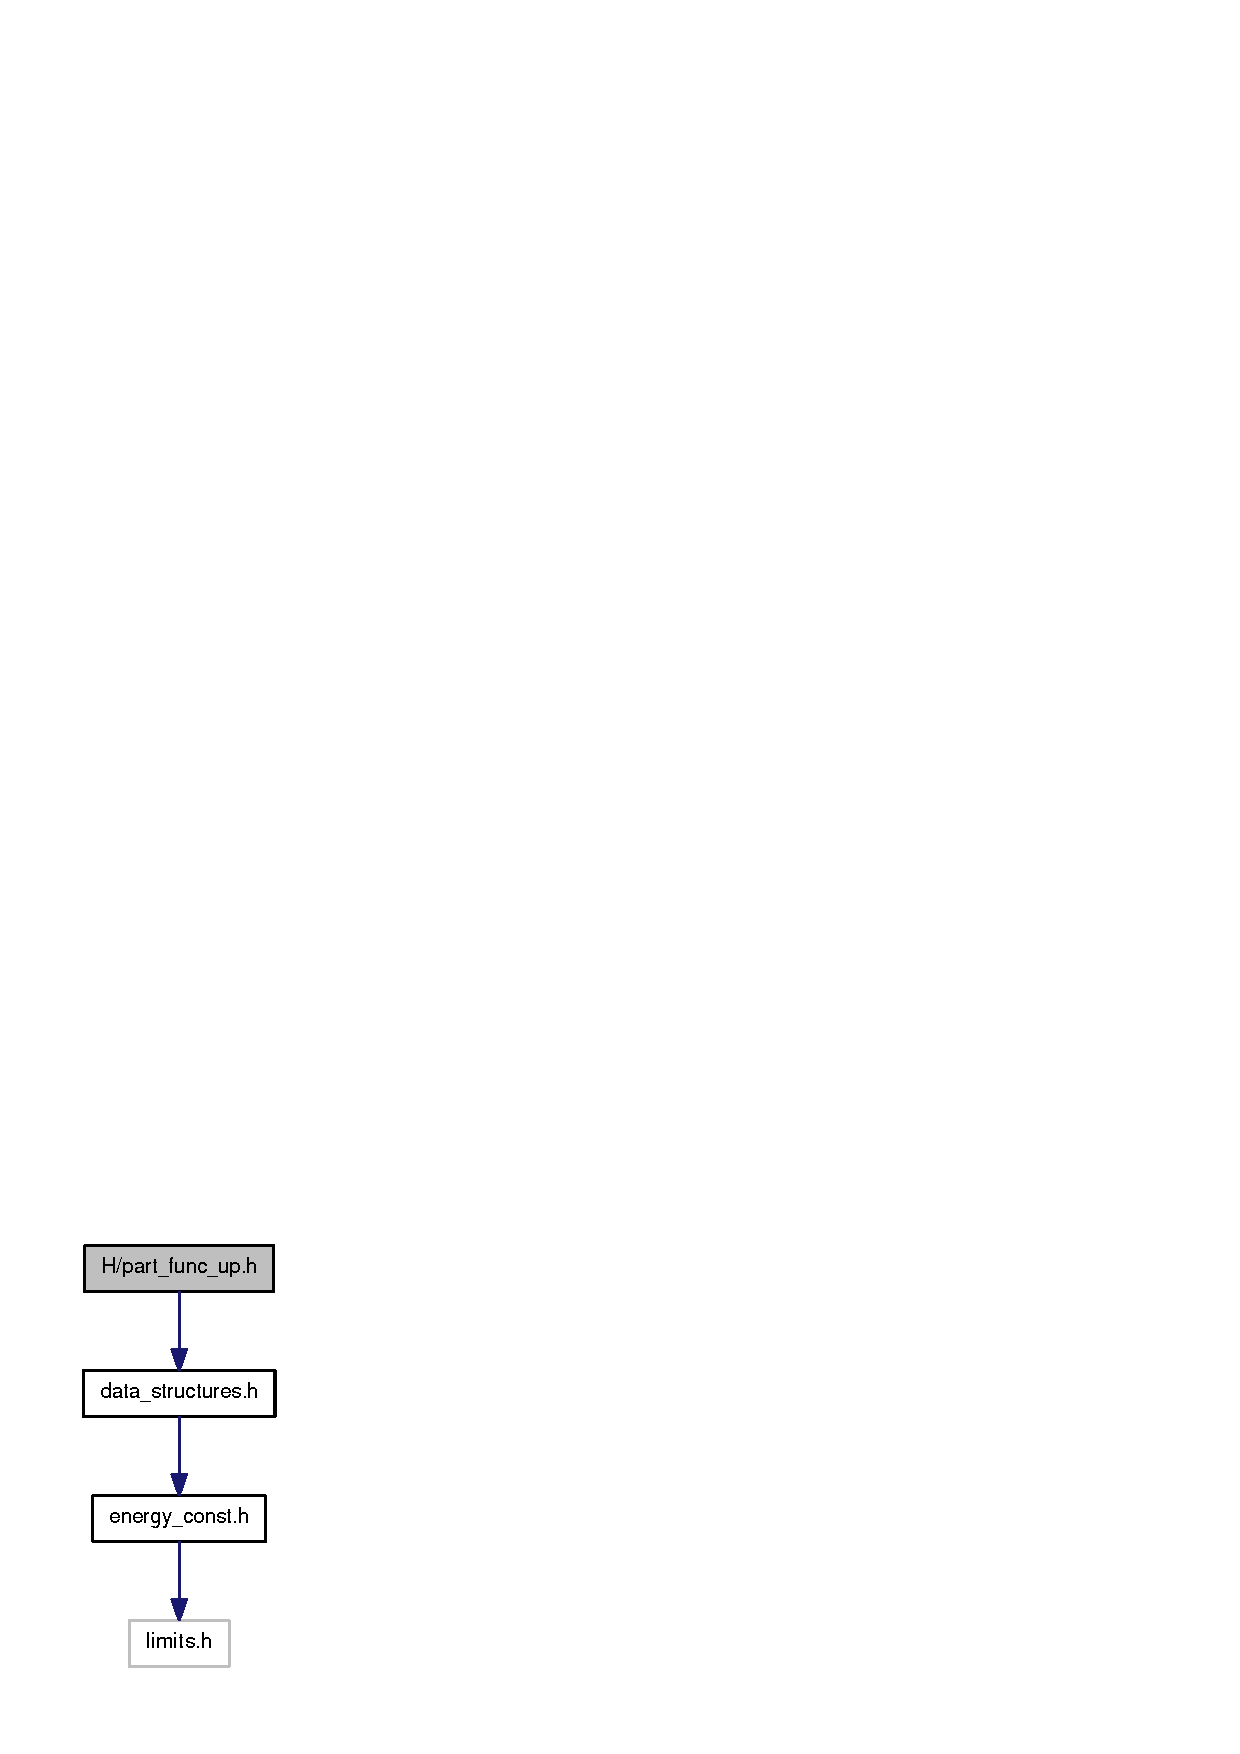
\includegraphics[width=68pt]{part__func__up_8h__incl}
\end{center}
\end{figure}
\subsection*{Functions}
\begin{DoxyCompactItemize}
\item 
\hyperlink{structpu__contrib}{pu\_\-contrib} $\ast$ \hyperlink{part__func__up_8h_a5b4ee40e190d2f633cd01cf0d2fe93cf}{pf\_\-unstru} (char $\ast$sequence, int max\_\-w)
\begin{DoxyCompactList}\small\item\em Calculate the partition function over all unpaired regions of a maximal length. \item\end{DoxyCompactList}\item 
\hyperlink{structinteract}{interact} $\ast$ \hyperlink{part__func__up_8h_a1aa0aa02bc3a724f87360c03097afd00}{pf\_\-interact} (const char $\ast$s1, const char $\ast$s2, \hyperlink{structpu__contrib}{pu\_\-contrib} $\ast$p\_\-c, \hyperlink{structpu__contrib}{pu\_\-contrib} $\ast$p\_\-c2, int max\_\-w, char $\ast$cstruc, int incr3, int incr5)
\begin{DoxyCompactList}\small\item\em Calculates the probability of a local interaction between two sequences. \item\end{DoxyCompactList}\item 
\hypertarget{part__func__up_8h_adde308fd5f696dc271b1532aa96fd12f}{
void \hyperlink{part__func__up_8h_adde308fd5f696dc271b1532aa96fd12f}{free\_\-interact} (\hyperlink{structinteract}{interact} $\ast$pin)}
\label{part__func__up_8h_adde308fd5f696dc271b1532aa96fd12f}

\begin{DoxyCompactList}\small\item\em Frees the output of function \hyperlink{part__func__up_8h_a1aa0aa02bc3a724f87360c03097afd00}{pf\_\-interact()}. \item\end{DoxyCompactList}\item 
\hypertarget{part__func__up_8h_ac20bd61824981d45ce0dc9934aa56df8}{
void \hyperlink{part__func__up_8h_ac20bd61824981d45ce0dc9934aa56df8}{free\_\-pu\_\-contrib\_\-struct} (\hyperlink{structpu__contrib}{pu\_\-contrib} $\ast$pu)}
\label{part__func__up_8h_ac20bd61824981d45ce0dc9934aa56df8}

\begin{DoxyCompactList}\small\item\em Frees the output of function \hyperlink{part__func__up_8h_a5b4ee40e190d2f633cd01cf0d2fe93cf}{pf\_\-unstru()}. \item\end{DoxyCompactList}\end{DoxyCompactItemize}


\subsection{Detailed Description}
Partition Function Cofolding as stepwise process. In this approach to cofolding the interaction between two RNA molecules is seen as a stepwise process. In a first step, the target molecule has to adopt a structure in which a binding site is accessible. In a second step, the ligand molecule will hybridize with a region accessible to an interaction. Consequently the algorithm is designed as a two step process: The first step is the calculation of the probability that a region within the target is unpaired, or equivalently, the calculation of the free energy needed to expose a region. In the second step we compute the free energy of an interaction for every possible binding site. 

\subsection{Function Documentation}
\hypertarget{part__func__up_8h_a5b4ee40e190d2f633cd01cf0d2fe93cf}{
\index{part\_\-func\_\-up.h@{part\_\-func\_\-up.h}!pf\_\-unstru@{pf\_\-unstru}}
\index{pf\_\-unstru@{pf\_\-unstru}!part_func_up.h@{part\_\-func\_\-up.h}}
\subsubsection[{pf\_\-unstru}]{\setlength{\rightskip}{0pt plus 5cm}{\bf pu\_\-contrib}$\ast$ pf\_\-unstru (char $\ast$ {\em sequence}, \/  int {\em max\_\-w})}}
\label{part__func__up_8h_a5b4ee40e190d2f633cd01cf0d2fe93cf}


Calculate the partition function over all unpaired regions of a maximal length. 

You have to call function \hyperlink{part__func_8h_adc3db3d98742427e7001a7fd36ef28c2}{pf\_\-fold()} providing the same sequence before calling \hyperlink{part__func__up_8h_a5b4ee40e190d2f633cd01cf0d2fe93cf}{pf\_\-unstru()}. If you want to calculate unpaired regions for a constrained structure, set variable 'structure' in function 'pf\_\-fold()' to the constrain string. It returns a \hyperlink{structpu__contrib}{pu\_\-contrib} struct containing four arrays of dimension \mbox{[}i = 1 to length(sequence)\mbox{]}\mbox{[}j = 0 to u-\/1\mbox{]} containing all possible contributions to the probabilities of unpaired regions of maximum length u. Each array in \hyperlink{structpu__contrib}{pu\_\-contrib} contains one of the contributions to the total probability of being unpaired: The probability of being unpaired within an exterior loop is in array \hyperlink{structpu__contrib}{pu\_\-contrib}-\/$>$E, the probability of being unpaired within a hairpin loop is in array \hyperlink{structpu__contrib}{pu\_\-contrib}-\/$>$H, the probability of being unpaired within an interior loop is in array \hyperlink{structpu__contrib}{pu\_\-contrib}-\/$>$I and probability of being unpaired within a multi-\/loop is in array \hyperlink{structpu__contrib}{pu\_\-contrib}-\/$>$M. The total probability of being unpaired is the sum of the four arrays of \hyperlink{structpu__contrib}{pu\_\-contrib}.

This function frees everything allocated automatically. To free the output structure call free\_\-pu\_\-contrib().


\begin{DoxyParams}{Parameters}
\item[{\em sequence}]
\begin{DoxyParams}{Parameters}
\item[{\em max\_\-w}]\begin{DoxyReturn}{Returns}

\end{DoxyReturn}
\end{DoxyParams}
\end{DoxyParams}
\hypertarget{part__func__up_8h_a1aa0aa02bc3a724f87360c03097afd00}{
\index{part\_\-func\_\-up.h@{part\_\-func\_\-up.h}!pf\_\-interact@{pf\_\-interact}}
\index{pf\_\-interact@{pf\_\-interact}!part_func_up.h@{part\_\-func\_\-up.h}}
\subsubsection[{pf\_\-interact}]{\setlength{\rightskip}{0pt plus 5cm}{\bf interact}$\ast$ pf\_\-interact (const char $\ast$ {\em s1}, \/  const char $\ast$ {\em s2}, \/  {\bf pu\_\-contrib} $\ast$ {\em p\_\-c}, \/  {\bf pu\_\-contrib} $\ast$ {\em p\_\-c2}, \/  int {\em max\_\-w}, \/  char $\ast$ {\em cstruc}, \/  int {\em incr3}, \/  int {\em incr5})}}
\label{part__func__up_8h_a1aa0aa02bc3a724f87360c03097afd00}


Calculates the probability of a local interaction between two sequences. 

The function considers the probability that the region of interaction is unpaired within 's1' and 's2'. The longer sequence has to be given as 's1'. The shorter sequence has to be given as 's2'. Function \hyperlink{part__func__up_8h_a5b4ee40e190d2f633cd01cf0d2fe93cf}{pf\_\-unstru()} has to be called for 's1' and 's2', where the probabilities of being unpaired have to be given in 'p\_\-c' and 'p\_\-c2', respectively. If you do not want to include the probabilities of being unpaired for 's2' set 'p\_\-c2' to NULL. If variable 'cstruc' is not NULL, constrained folding is done: The available constrains for intermolecular interaction are: '.' (no constrain), 'x' (the base has no intermolecular interaction) and '$|$' (the corresponding base has to be paired intermolecularily).\par
 The parameter 'w' determines the maximal length of the interaction. The parameters 'incr5' and 'incr3' allows inclusion of unpaired residues left ('incr5') and right ('incr3') of the region of interaction in 's1'. If the 'incr' options are used, function \hyperlink{part__func__up_8h_a5b4ee40e190d2f633cd01cf0d2fe93cf}{pf\_\-unstru()} has to be called with w=w+incr5+incr3 for the longer sequence 's1'.

It returns a structure of type \hyperlink{structinteract}{interact} which contains the probability of the best local interaction including residue i in Pi and the minimum free energy in Gi, where i is the position in sequence 's1'. The member Gikjl of structure \hyperlink{structinteract}{interact} is the best interaction between region \mbox{[}k,i\mbox{]} k$<$i in longer sequence 's1' and region \mbox{[}j,l\mbox{]} j$<$l in 's2'. Gikjl\_\-wo is Gikjl without the probability of beeing unpaired.\par
 Use \hyperlink{part__func__up_8h_adde308fd5f696dc271b1532aa96fd12f}{free\_\-interact()} to free the returned structure, all other stuff is freed inside \hyperlink{part__func__up_8h_a1aa0aa02bc3a724f87360c03097afd00}{pf\_\-interact()}.


\begin{DoxyParams}{Parameters}
\item[{\em s1}]
\begin{DoxyParams}{Parameters}
\item[{\em s2}]
\begin{DoxyParams}{Parameters}
\item[{\em p\_\-c}]
\begin{DoxyParams}{Parameters}
\item[{\em p\_\-c2}]
\begin{DoxyParams}{Parameters}
\item[{\em max\_\-w}]
\begin{DoxyParams}{Parameters}
\item[{\em cstruc}]
\begin{DoxyParams}{Parameters}
\item[{\em incr3}]
\begin{DoxyParams}{Parameters}
\item[{\em incr5}]\begin{DoxyReturn}{Returns}

\end{DoxyReturn}
\end{DoxyParams}
\end{DoxyParams}
\end{DoxyParams}
\end{DoxyParams}
\end{DoxyParams}
\end{DoxyParams}
\end{DoxyParams}
\end{DoxyParams}

\hypertarget{plot__layouts_8h}{
\section{H/plot\_\-layouts.h File Reference}
\label{plot__layouts_8h}\index{H/plot\_\-layouts.h@{H/plot\_\-layouts.h}}
}


Secondary structure plot layout algorithms.  


Include dependency graph for plot\_\-layouts.h:\nopagebreak
\begin{figure}[H]
\begin{center}
\leavevmode
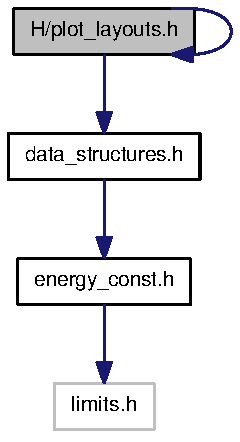
\includegraphics[width=75pt]{plot__layouts_8h__incl}
\end{center}
\end{figure}
This graph shows which files directly or indirectly include this file:\nopagebreak
\begin{figure}[H]
\begin{center}
\leavevmode

\includegraphics[width=74pt]{plot__layouts_8h__dep__incl}
\end{center}
\end{figure}
\subsection*{Defines}
\begin{DoxyCompactItemize}
\item 
\#define \hyperlink{plot__layouts_8h_ae6d17b9f0a53cf5205a9181e0f8422e9}{VRNA\_\-PLOT\_\-TYPE\_\-SIMPLE}~0
\begin{DoxyCompactList}\small\item\em Definition of Plot type {\itshape simple\/} \item\end{DoxyCompactList}\item 
\#define \hyperlink{plot__layouts_8h_a94d4c863ecac2f220f76658afb92f964}{VRNA\_\-PLOT\_\-TYPE\_\-NAVIEW}~1
\begin{DoxyCompactList}\small\item\em Definition of Plot type {\itshape Naview\/} \item\end{DoxyCompactList}\item 
\#define \hyperlink{plot__layouts_8h_a8c9eac631348da92136c8363ecdd9fb9}{VRNA\_\-PLOT\_\-TYPE\_\-CIRCULAR}~2
\begin{DoxyCompactList}\small\item\em Definition of Plot type {\itshape Circular\/} \item\end{DoxyCompactList}\end{DoxyCompactItemize}
\subsection*{Functions}
\begin{DoxyCompactItemize}
\item 
int \hyperlink{plot__layouts_8h_af4b9173e7d3fd361c3c85e6def194123}{simple\_\-xy\_\-coordinates} (short $\ast$pair\_\-table, float $\ast$X, float $\ast$Y)
\begin{DoxyCompactList}\small\item\em Calculate nucleotide coordinates for secondary structure plot the {\itshape Simple way\/} \item\end{DoxyCompactList}\item 
int \hyperlink{plot__layouts_8h_ac4ea13d35308f09940178d2b05a248c2}{simple\_\-circplot\_\-coordinates} (short $\ast$pair\_\-table, float $\ast$x, float $\ast$y)
\begin{DoxyCompactList}\small\item\em Calculate nucleotide coordinates for {\itshape Circular Plot\/} \item\end{DoxyCompactList}\end{DoxyCompactItemize}
\subsection*{Variables}
\begin{DoxyCompactItemize}
\item 
int \hyperlink{plot__layouts_8h_a5964c4581431b098b80027d6e14dcdd4}{rna\_\-plot\_\-type}
\begin{DoxyCompactList}\small\item\em Switch for changing the secondary structure layout algorithm. \item\end{DoxyCompactList}\end{DoxyCompactItemize}


\subsection{Detailed Description}
Secondary structure plot layout algorithms. c Ronny Lorenz The ViennaRNA Package 

\subsection{Define Documentation}
\hypertarget{plot__layouts_8h_ae6d17b9f0a53cf5205a9181e0f8422e9}{
\index{plot\_\-layouts.h@{plot\_\-layouts.h}!VRNA\_\-PLOT\_\-TYPE\_\-SIMPLE@{VRNA\_\-PLOT\_\-TYPE\_\-SIMPLE}}
\index{VRNA\_\-PLOT\_\-TYPE\_\-SIMPLE@{VRNA\_\-PLOT\_\-TYPE\_\-SIMPLE}!plot_layouts.h@{plot\_\-layouts.h}}
\subsubsection[{VRNA\_\-PLOT\_\-TYPE\_\-SIMPLE}]{\setlength{\rightskip}{0pt plus 5cm}\#define VRNA\_\-PLOT\_\-TYPE\_\-SIMPLE~0}}
\label{plot__layouts_8h_ae6d17b9f0a53cf5205a9181e0f8422e9}


Definition of Plot type {\itshape simple\/} 

This is the plot type definition for several RNA structure plotting functions telling them to use {\bfseries Simple} plotting algorithm

\begin{DoxySeeAlso}{See also}
\hyperlink{plot__layouts_8h_a5964c4581431b098b80027d6e14dcdd4}{rna\_\-plot\_\-type}, \hyperlink{PS__dot_8h_a47856b2504b566588785597b6ebb8271}{PS\_\-rna\_\-plot\_\-a()}, \hyperlink{PS__dot_8h_a0873c7cc4cd7a11c9a2cea19dde7e9c9}{PS\_\-rna\_\-plot()}, \hyperlink{PS__dot_8h_ae7853539b5df98f294b4af434e979304}{svg\_\-rna\_\-plot()}, \hyperlink{PS__dot_8h_a70834bc8c0aad4fe6824ff76ccb8f329}{gmlRNA()}, \hyperlink{PS__dot_8h_add368528755f9a830727b680243541df}{ssv\_\-rna\_\-plot()}, \hyperlink{PS__dot_8h_a2f6d5953e6a323df898896b8d6614483}{xrna\_\-plot()} 
\end{DoxySeeAlso}
\hypertarget{plot__layouts_8h_a94d4c863ecac2f220f76658afb92f964}{
\index{plot\_\-layouts.h@{plot\_\-layouts.h}!VRNA\_\-PLOT\_\-TYPE\_\-NAVIEW@{VRNA\_\-PLOT\_\-TYPE\_\-NAVIEW}}
\index{VRNA\_\-PLOT\_\-TYPE\_\-NAVIEW@{VRNA\_\-PLOT\_\-TYPE\_\-NAVIEW}!plot_layouts.h@{plot\_\-layouts.h}}
\subsubsection[{VRNA\_\-PLOT\_\-TYPE\_\-NAVIEW}]{\setlength{\rightskip}{0pt plus 5cm}\#define VRNA\_\-PLOT\_\-TYPE\_\-NAVIEW~1}}
\label{plot__layouts_8h_a94d4c863ecac2f220f76658afb92f964}


Definition of Plot type {\itshape Naview\/} 

This is the plot type definition for several RNA structure plotting functions telling them to use {\bfseries Naview} plotting algorithm

\begin{DoxySeeAlso}{See also}
\hyperlink{plot__layouts_8h_a5964c4581431b098b80027d6e14dcdd4}{rna\_\-plot\_\-type}, \hyperlink{PS__dot_8h_a47856b2504b566588785597b6ebb8271}{PS\_\-rna\_\-plot\_\-a()}, \hyperlink{PS__dot_8h_a0873c7cc4cd7a11c9a2cea19dde7e9c9}{PS\_\-rna\_\-plot()}, \hyperlink{PS__dot_8h_ae7853539b5df98f294b4af434e979304}{svg\_\-rna\_\-plot()}, \hyperlink{PS__dot_8h_a70834bc8c0aad4fe6824ff76ccb8f329}{gmlRNA()}, \hyperlink{PS__dot_8h_add368528755f9a830727b680243541df}{ssv\_\-rna\_\-plot()}, \hyperlink{PS__dot_8h_a2f6d5953e6a323df898896b8d6614483}{xrna\_\-plot()} 
\end{DoxySeeAlso}
\hypertarget{plot__layouts_8h_a8c9eac631348da92136c8363ecdd9fb9}{
\index{plot\_\-layouts.h@{plot\_\-layouts.h}!VRNA\_\-PLOT\_\-TYPE\_\-CIRCULAR@{VRNA\_\-PLOT\_\-TYPE\_\-CIRCULAR}}
\index{VRNA\_\-PLOT\_\-TYPE\_\-CIRCULAR@{VRNA\_\-PLOT\_\-TYPE\_\-CIRCULAR}!plot_layouts.h@{plot\_\-layouts.h}}
\subsubsection[{VRNA\_\-PLOT\_\-TYPE\_\-CIRCULAR}]{\setlength{\rightskip}{0pt plus 5cm}\#define VRNA\_\-PLOT\_\-TYPE\_\-CIRCULAR~2}}
\label{plot__layouts_8h_a8c9eac631348da92136c8363ecdd9fb9}


Definition of Plot type {\itshape Circular\/} 

This is the plot type definition for several RNA structure plotting functions telling them to produce a {\bfseries Circular plot}

\begin{DoxySeeAlso}{See also}
\hyperlink{plot__layouts_8h_a5964c4581431b098b80027d6e14dcdd4}{rna\_\-plot\_\-type}, \hyperlink{PS__dot_8h_a47856b2504b566588785597b6ebb8271}{PS\_\-rna\_\-plot\_\-a()}, \hyperlink{PS__dot_8h_a0873c7cc4cd7a11c9a2cea19dde7e9c9}{PS\_\-rna\_\-plot()}, \hyperlink{PS__dot_8h_ae7853539b5df98f294b4af434e979304}{svg\_\-rna\_\-plot()}, \hyperlink{PS__dot_8h_a70834bc8c0aad4fe6824ff76ccb8f329}{gmlRNA()}, \hyperlink{PS__dot_8h_add368528755f9a830727b680243541df}{ssv\_\-rna\_\-plot()}, \hyperlink{PS__dot_8h_a2f6d5953e6a323df898896b8d6614483}{xrna\_\-plot()} 
\end{DoxySeeAlso}


\subsection{Function Documentation}
\hypertarget{plot__layouts_8h_af4b9173e7d3fd361c3c85e6def194123}{
\index{plot\_\-layouts.h@{plot\_\-layouts.h}!simple\_\-xy\_\-coordinates@{simple\_\-xy\_\-coordinates}}
\index{simple\_\-xy\_\-coordinates@{simple\_\-xy\_\-coordinates}!plot_layouts.h@{plot\_\-layouts.h}}
\subsubsection[{simple\_\-xy\_\-coordinates}]{\setlength{\rightskip}{0pt plus 5cm}int simple\_\-xy\_\-coordinates (short $\ast$ {\em pair\_\-table}, \/  float $\ast$ {\em X}, \/  float $\ast$ {\em Y})}}
\label{plot__layouts_8h_af4b9173e7d3fd361c3c85e6def194123}


Calculate nucleotide coordinates for secondary structure plot the {\itshape Simple way\/} 

\begin{DoxySeeAlso}{See also}
\hyperlink{utils_8h_a89c32307ee50a0026f4a3131fac0845a}{make\_\-pair\_\-table()}, \hyperlink{plot__layouts_8h_a5964c4581431b098b80027d6e14dcdd4}{rna\_\-plot\_\-type}, \hyperlink{plot__layouts_8h_ac4ea13d35308f09940178d2b05a248c2}{simple\_\-circplot\_\-coordinates()}, naview\_\-xy\_\-coordinates(), \hyperlink{PS__dot_8h_a47856b2504b566588785597b6ebb8271}{PS\_\-rna\_\-plot\_\-a()}, \hyperlink{PS__dot_8h_a0873c7cc4cd7a11c9a2cea19dde7e9c9}{PS\_\-rna\_\-plot}, \hyperlink{PS__dot_8h_ae7853539b5df98f294b4af434e979304}{svg\_\-rna\_\-plot()}
\end{DoxySeeAlso}

\begin{DoxyParams}{Parameters}
\item[{\em pair\_\-table}]The pair table of the secondary structure 
\begin{DoxyParams}{Parameters}
\item[{\em X}]a pointer to an array with enough allocated space to hold the x coordinates 
\begin{DoxyParams}{Parameters}
\item[{\em Y}]a pointer to an array with enough allocated space to hold the y coordinates \begin{DoxyReturn}{Returns}
length of sequence on success, 0 otherwise 
\end{DoxyReturn}
\end{DoxyParams}
\end{DoxyParams}
\end{DoxyParams}
\hypertarget{plot__layouts_8h_ac4ea13d35308f09940178d2b05a248c2}{
\index{plot\_\-layouts.h@{plot\_\-layouts.h}!simple\_\-circplot\_\-coordinates@{simple\_\-circplot\_\-coordinates}}
\index{simple\_\-circplot\_\-coordinates@{simple\_\-circplot\_\-coordinates}!plot_layouts.h@{plot\_\-layouts.h}}
\subsubsection[{simple\_\-circplot\_\-coordinates}]{\setlength{\rightskip}{0pt plus 5cm}int simple\_\-circplot\_\-coordinates (short $\ast$ {\em pair\_\-table}, \/  float $\ast$ {\em x}, \/  float $\ast$ {\em y})}}
\label{plot__layouts_8h_ac4ea13d35308f09940178d2b05a248c2}


Calculate nucleotide coordinates for {\itshape Circular Plot\/} 

This function calculates the coordinates of nucleotides mapped in equal distancies onto a unit circle.

\begin{DoxyNote}{Note}
In order to draw nice arcs using quadratic bezier curves that connect base pairs one may calculate a second tangential point $P^t$ in addition to the actual R$^{\mbox{2}}$  coordinates. the simplest way to do so may be to compute a radius scaling factor $rs$ in the interval $[0,1]$ that weights the proportion of base pair span to the actual length of the sequence. This scaling factor can then be used to calculate the coordinates for $P^t$, i.e. $ P^{t}_x[i] = X[i] * rs$ and $P^{t}_y[i] = Y[i] * rs$.
\end{DoxyNote}
\begin{DoxySeeAlso}{See also}
\hyperlink{utils_8h_a89c32307ee50a0026f4a3131fac0845a}{make\_\-pair\_\-table()}, \hyperlink{plot__layouts_8h_a5964c4581431b098b80027d6e14dcdd4}{rna\_\-plot\_\-type}, \hyperlink{plot__layouts_8h_af4b9173e7d3fd361c3c85e6def194123}{simple\_\-xy\_\-coordinates()}, naview\_\-xy\_\-coordinates(), \hyperlink{PS__dot_8h_a47856b2504b566588785597b6ebb8271}{PS\_\-rna\_\-plot\_\-a()}, \hyperlink{PS__dot_8h_a0873c7cc4cd7a11c9a2cea19dde7e9c9}{PS\_\-rna\_\-plot}, \hyperlink{PS__dot_8h_ae7853539b5df98f294b4af434e979304}{svg\_\-rna\_\-plot()}
\end{DoxySeeAlso}

\begin{DoxyParams}{Parameters}
\item[{\em pair\_\-table}]The pair table of the secondary structure 
\begin{DoxyParams}{Parameters}
\item[{\em x}]a pointer to an array with enough allocated space to hold the x coordinates 
\begin{DoxyParams}{Parameters}
\item[{\em y}]a pointer to an array with enough allocated space to hold the y coordinates \begin{DoxyReturn}{Returns}
length of sequence on success, 0 otherwise 
\end{DoxyReturn}
\end{DoxyParams}
\end{DoxyParams}
\end{DoxyParams}


\subsection{Variable Documentation}
\hypertarget{plot__layouts_8h_a5964c4581431b098b80027d6e14dcdd4}{
\index{plot\_\-layouts.h@{plot\_\-layouts.h}!rna\_\-plot\_\-type@{rna\_\-plot\_\-type}}
\index{rna\_\-plot\_\-type@{rna\_\-plot\_\-type}!plot_layouts.h@{plot\_\-layouts.h}}
\subsubsection[{rna\_\-plot\_\-type}]{\setlength{\rightskip}{0pt plus 5cm}int {\bf rna\_\-plot\_\-type}}}
\label{plot__layouts_8h_a5964c4581431b098b80027d6e14dcdd4}


Switch for changing the secondary structure layout algorithm. 

Current possibility are 0 for a simple radial drawing or 1 for the modified radial drawing taken from the {\itshape naview\/} program of \hyperlink{mp__ref_bruccoleri_88}{Bruccoleri \& Heinrich (1988)}.

\begin{DoxyNote}{Note}
To provide thread safety please do not rely on this global variable in future implementations but pass a plot type flag directly to the function that decides which layout algorithm it may use!
\end{DoxyNote}
\begin{DoxySeeAlso}{See also}
\hyperlink{plot__layouts_8h_ae6d17b9f0a53cf5205a9181e0f8422e9}{VRNA\_\-PLOT\_\-TYPE\_\-SIMPLE}, \hyperlink{plot__layouts_8h_a94d4c863ecac2f220f76658afb92f964}{VRNA\_\-PLOT\_\-TYPE\_\-NAVIEW}, \hyperlink{plot__layouts_8h_a8c9eac631348da92136c8363ecdd9fb9}{VRNA\_\-PLOT\_\-TYPE\_\-CIRCULAR} 
\end{DoxySeeAlso}

\hypertarget{profiledist_8h}{
\section{H/profiledist.h File Reference}
\label{profiledist_8h}\index{H/profiledist.h@{H/profiledist.h}}
}
Include dependency graph for profiledist.h:\nopagebreak
\begin{figure}[H]
\begin{center}
\leavevmode
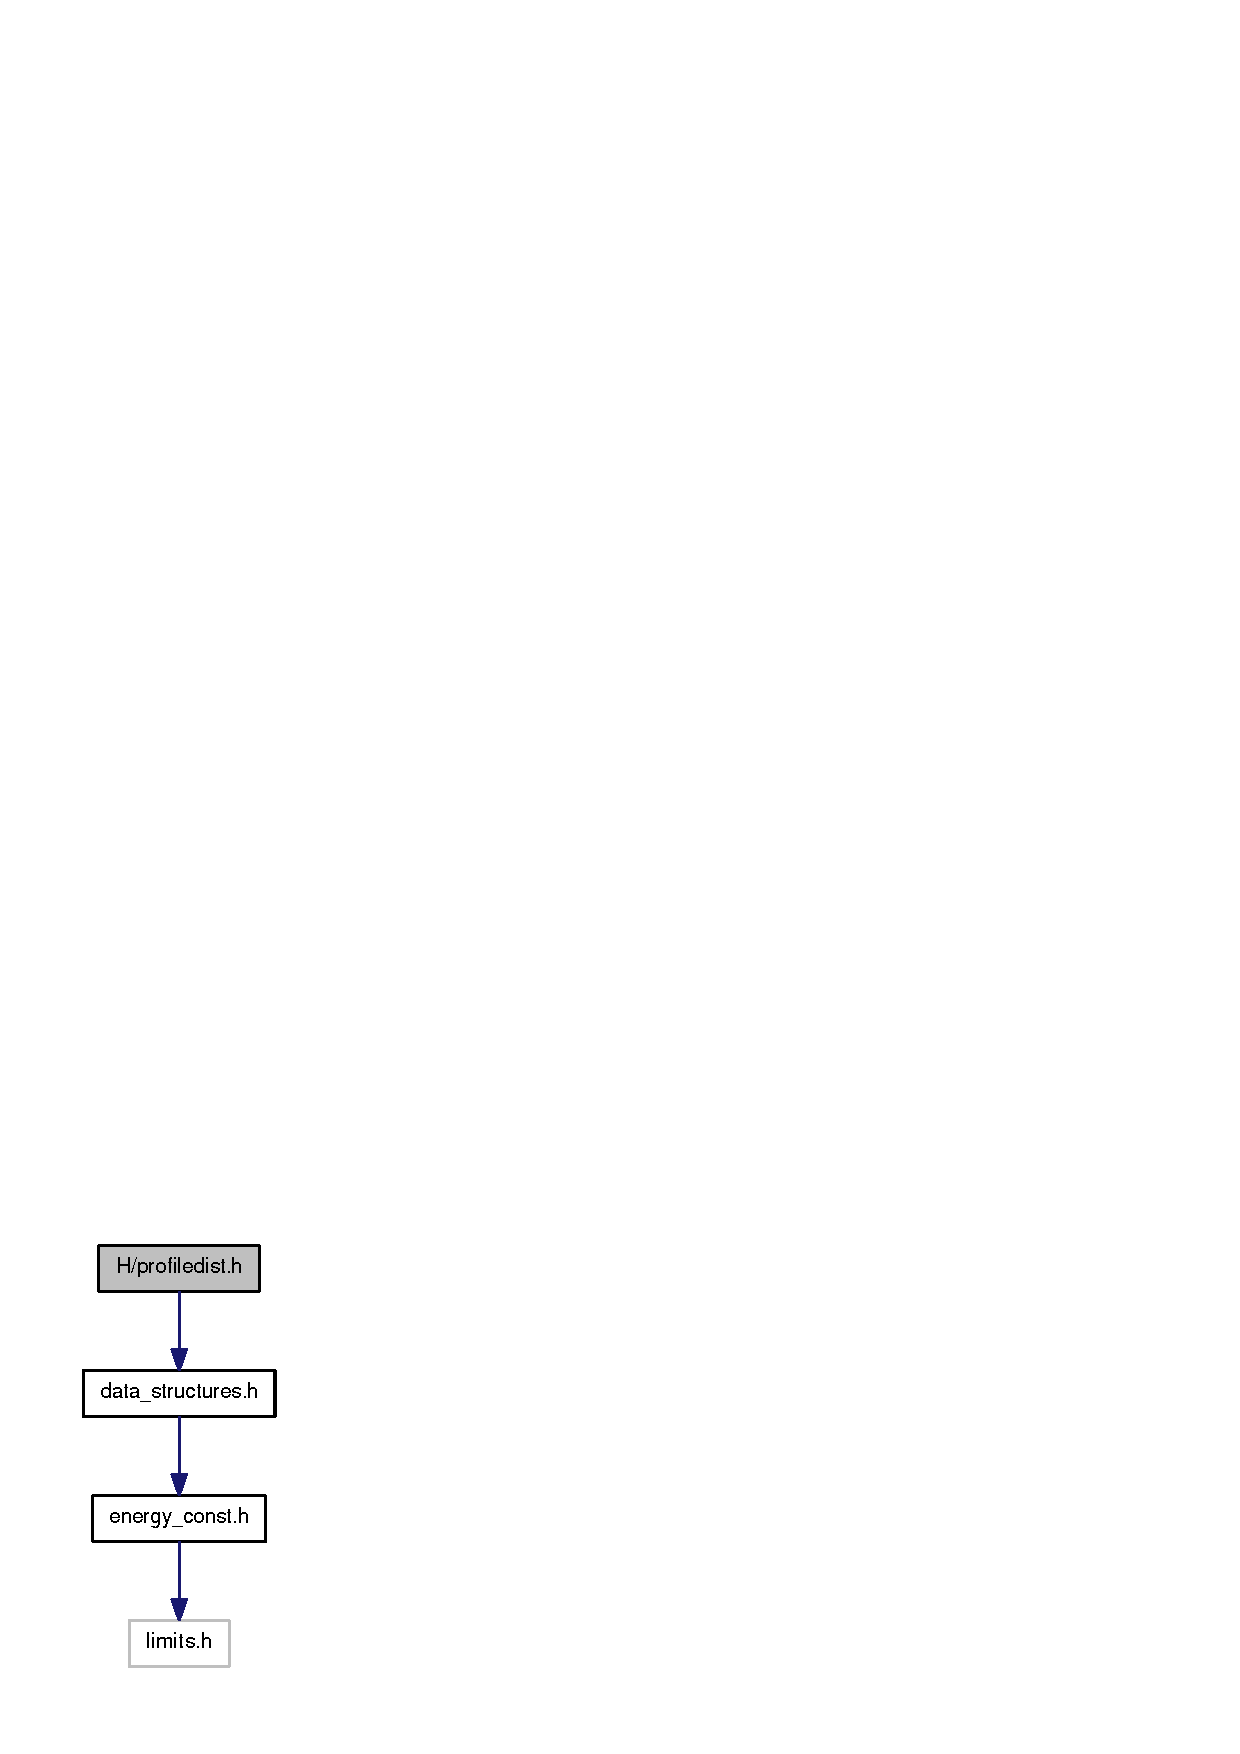
\includegraphics[width=68pt]{profiledist_8h__incl}
\end{center}
\end{figure}
\subsection*{Functions}
\begin{DoxyCompactItemize}
\item 
float \hyperlink{profiledist_8h_abe75e90e00a1e5dd8862944ed53dad5d}{profile\_\-edit\_\-distance} (const float $\ast$T1, const float $\ast$T2)
\begin{DoxyCompactList}\small\item\em Align the 2 probability profiles T1, T2\par
. \item\end{DoxyCompactList}\item 
float $\ast$ \hyperlink{profiledist_8h_a3dff26e707a2a2e65a0f759caabde6e7}{Make\_\-bp\_\-profile\_\-bppm} (FLT\_\-OR\_\-DBL $\ast$bppm, int length)
\begin{DoxyCompactList}\small\item\em condense pair probability matrix into a vector containing probabilities for upstream paired, downstream paired and unpaired. \item\end{DoxyCompactList}\item 
\hypertarget{profiledist_8h_a8e0b4fe3698b3502945116ecc0ba6160}{
void \hyperlink{profiledist_8h_a8e0b4fe3698b3502945116ecc0ba6160}{print\_\-bppm} (const float $\ast$T)}
\label{profiledist_8h_a8e0b4fe3698b3502945116ecc0ba6160}

\begin{DoxyCompactList}\small\item\em print string representation of probability profile \item\end{DoxyCompactList}\item 
void \hyperlink{profiledist_8h_a9b0b84a5a45761bf42d7c835dcdb3b85}{free\_\-profile} (float $\ast$T)
\begin{DoxyCompactList}\small\item\em free space allocated in Make\_\-bp\_\-profile \item\end{DoxyCompactList}\item 
float $\ast$ \hyperlink{profiledist_8h_a904c7eaf4a2413567c00ac4891749d18}{Make\_\-bp\_\-profile} (int length)
\end{DoxyCompactItemize}


\subsection{Detailed Description}


\subsection{Function Documentation}
\hypertarget{profiledist_8h_abe75e90e00a1e5dd8862944ed53dad5d}{
\index{profiledist.h@{profiledist.h}!profile\_\-edit\_\-distance@{profile\_\-edit\_\-distance}}
\index{profile\_\-edit\_\-distance@{profile\_\-edit\_\-distance}!profiledist.h@{profiledist.h}}
\subsubsection[{profile\_\-edit\_\-distance}]{\setlength{\rightskip}{0pt plus 5cm}float profile\_\-edit\_\-distance (const float $\ast$ {\em T1}, \/  const float $\ast$ {\em T2})}}
\label{profiledist_8h_abe75e90e00a1e5dd8862944ed53dad5d}


Align the 2 probability profiles T1, T2\par
. 

This is like a Needleman-\/Wunsch alignment, we should really use affine gap-\/costs ala Gotoh \hypertarget{profiledist_8h_a3dff26e707a2a2e65a0f759caabde6e7}{
\index{profiledist.h@{profiledist.h}!Make\_\-bp\_\-profile\_\-bppm@{Make\_\-bp\_\-profile\_\-bppm}}
\index{Make\_\-bp\_\-profile\_\-bppm@{Make\_\-bp\_\-profile\_\-bppm}!profiledist.h@{profiledist.h}}
\subsubsection[{Make\_\-bp\_\-profile\_\-bppm}]{\setlength{\rightskip}{0pt plus 5cm}float$\ast$ Make\_\-bp\_\-profile\_\-bppm (FLT\_\-OR\_\-DBL $\ast$ {\em bppm}, \/  int {\em length})}}
\label{profiledist_8h_a3dff26e707a2a2e65a0f759caabde6e7}


condense pair probability matrix into a vector containing probabilities for upstream paired, downstream paired and unpaired. 

This resulting probability profile is used as input for profile\_\-edit\_\-distance


\begin{DoxyParams}{Parameters}
\item[{\em bppm}]A pointer to the base pair probability matrix 
\begin{DoxyParams}{Parameters}
\item[{\em length}]The length of the sequence \begin{DoxyReturn}{Returns}
The bp profile 
\end{DoxyReturn}
\end{DoxyParams}
\end{DoxyParams}
\hypertarget{profiledist_8h_a9b0b84a5a45761bf42d7c835dcdb3b85}{
\index{profiledist.h@{profiledist.h}!free\_\-profile@{free\_\-profile}}
\index{free\_\-profile@{free\_\-profile}!profiledist.h@{profiledist.h}}
\subsubsection[{free\_\-profile}]{\setlength{\rightskip}{0pt plus 5cm}void free\_\-profile (float $\ast$ {\em T})}}
\label{profiledist_8h_a9b0b84a5a45761bf42d7c835dcdb3b85}


free space allocated in Make\_\-bp\_\-profile 

Backward compatibility only. You can just use plain free() \hypertarget{profiledist_8h_a904c7eaf4a2413567c00ac4891749d18}{
\index{profiledist.h@{profiledist.h}!Make\_\-bp\_\-profile@{Make\_\-bp\_\-profile}}
\index{Make\_\-bp\_\-profile@{Make\_\-bp\_\-profile}!profiledist.h@{profiledist.h}}
\subsubsection[{Make\_\-bp\_\-profile}]{\setlength{\rightskip}{0pt plus 5cm}float$\ast$ Make\_\-bp\_\-profile (int {\em length})}}
\label{profiledist_8h_a904c7eaf4a2413567c00ac4891749d18}
\begin{DoxyNote}{Note}
This function is NOT threadsafe
\end{DoxyNote}
\begin{DoxySeeAlso}{See also}
\hyperlink{profiledist_8h_a3dff26e707a2a2e65a0f759caabde6e7}{Make\_\-bp\_\-profile\_\-bppm()}
\end{DoxySeeAlso}
\begin{Desc}
\item[\hyperlink{deprecated__deprecated000018}{Deprecated}]This function is deprecated and will be removed soon! See \hyperlink{profiledist_8h_a3dff26e707a2a2e65a0f759caabde6e7}{Make\_\-bp\_\-profile\_\-bppm()} for a replacement\end{Desc}

\hypertarget{PS__dot_8h}{
\section{H/PS\_\-dot.h File Reference}
\label{PS__dot_8h}\index{H/PS\_\-dot.h@{H/PS\_\-dot.h}}
}


Various functions for plotting RNA secondary structures, dot-\/plots and other visualizations.  


Include dependency graph for PS\_\-dot.h:\nopagebreak
\begin{figure}[H]
\begin{center}
\leavevmode
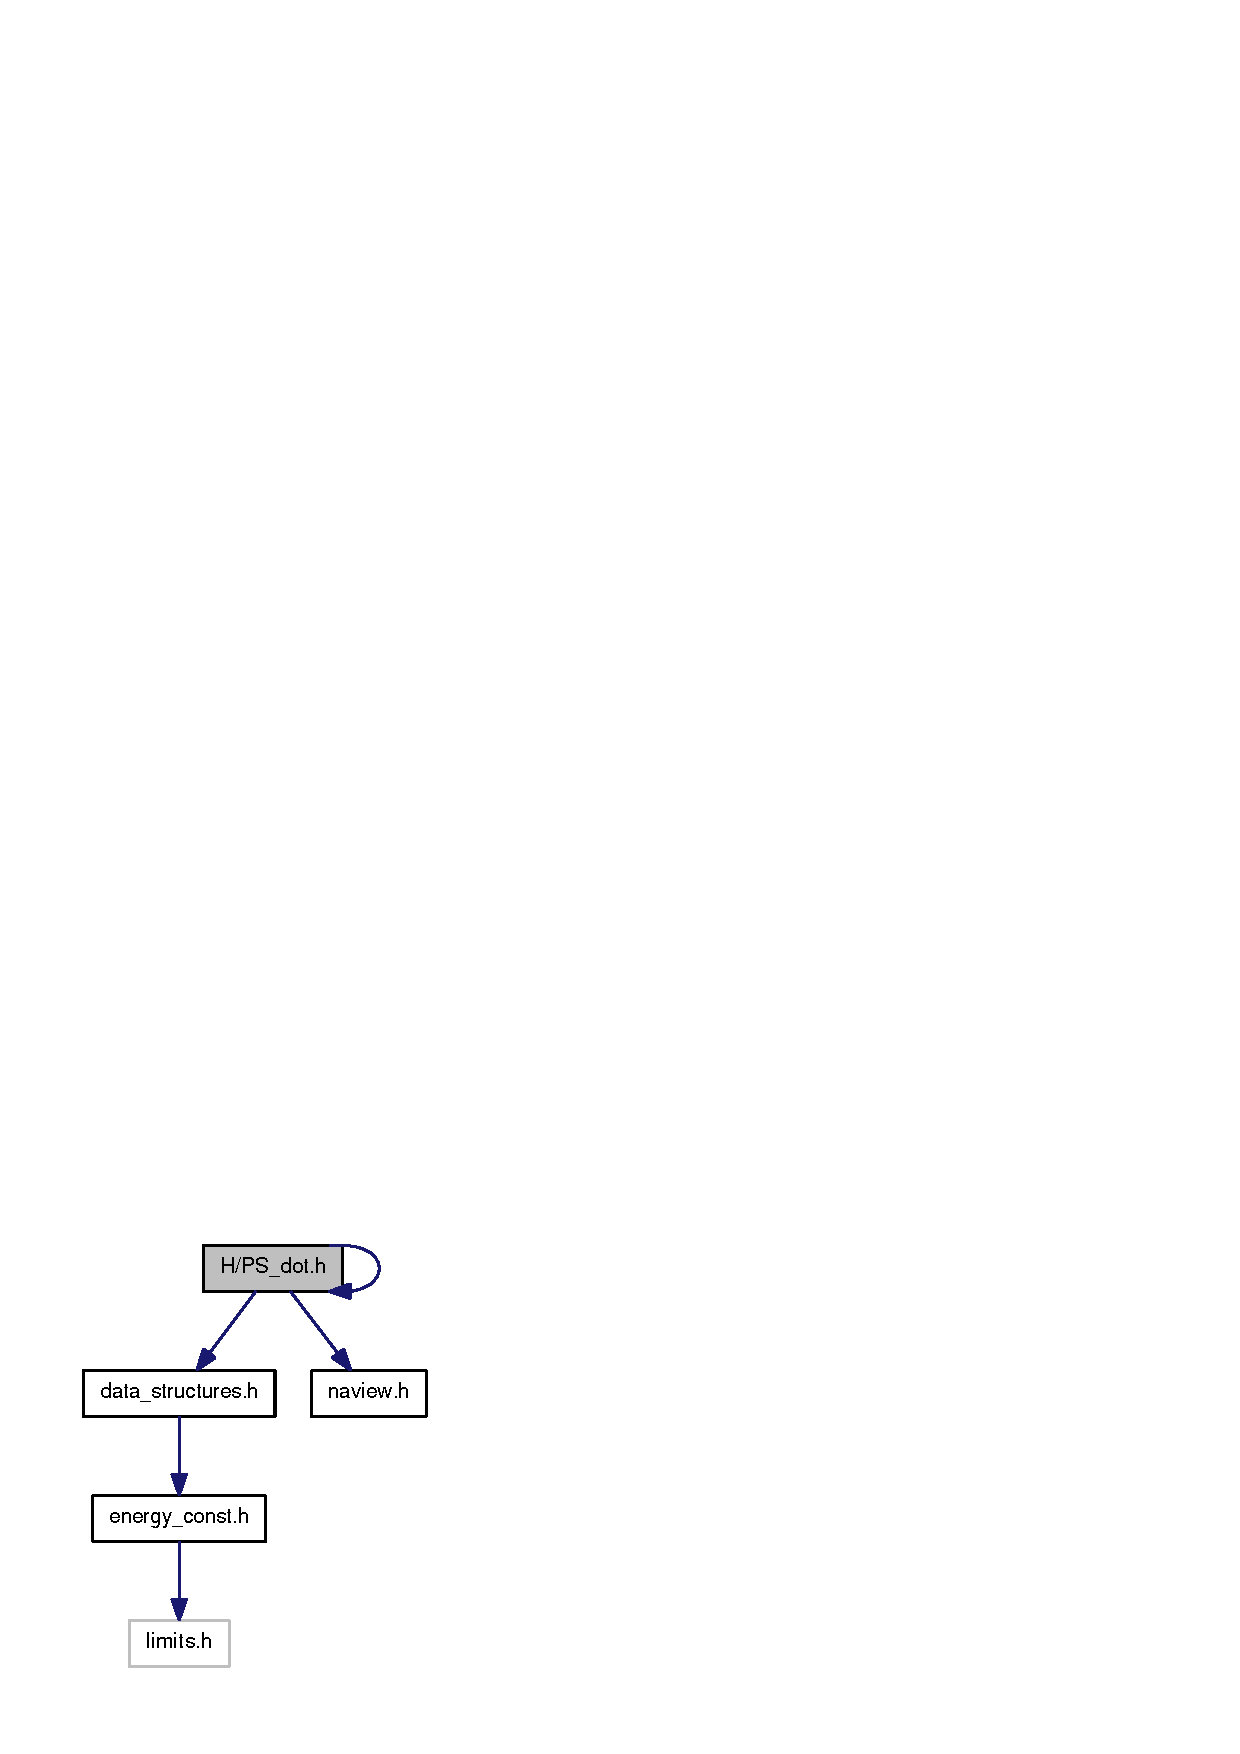
\includegraphics[width=104pt]{PS__dot_8h__incl}
\end{center}
\end{figure}
This graph shows which files directly or indirectly include this file:\nopagebreak
\begin{figure}[H]
\begin{center}
\leavevmode
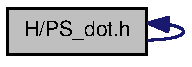
\includegraphics[width=64pt]{PS__dot_8h__dep__incl}
\end{center}
\end{figure}
\subsection*{Functions}
\begin{DoxyCompactItemize}
\item 
int \hyperlink{PS__dot_8h_a0873c7cc4cd7a11c9a2cea19dde7e9c9}{PS\_\-rna\_\-plot} (char $\ast$string, char $\ast$structure, char $\ast$file)
\begin{DoxyCompactList}\small\item\em Produce a secondary structure graph in PostScript and write it to 'filename'. \item\end{DoxyCompactList}\item 
int \hyperlink{PS__dot_8h_a47856b2504b566588785597b6ebb8271}{PS\_\-rna\_\-plot\_\-a} (char $\ast$string, char $\ast$structure, char $\ast$file, char $\ast$pre, char $\ast$post)
\begin{DoxyCompactList}\small\item\em Produce a secondary structure graph in PostScript including additional annotation macros and write it to 'filename'. \item\end{DoxyCompactList}\item 
int \hyperlink{PS__dot_8h_a70834bc8c0aad4fe6824ff76ccb8f329}{gmlRNA} (char $\ast$string, char $\ast$structure, char $\ast$ssfile, char option)
\begin{DoxyCompactList}\small\item\em Produce a secondary structure graph in Graph Meta Language (gml) and write it to a file. \item\end{DoxyCompactList}\item 
int \hyperlink{PS__dot_8h_add368528755f9a830727b680243541df}{ssv\_\-rna\_\-plot} (char $\ast$string, char $\ast$structure, char $\ast$ssfile)
\begin{DoxyCompactList}\small\item\em Produce a secondary structure graph in SStructView format. \item\end{DoxyCompactList}\item 
int \hyperlink{PS__dot_8h_ae7853539b5df98f294b4af434e979304}{svg\_\-rna\_\-plot} (char $\ast$string, char $\ast$structure, char $\ast$ssfile)
\begin{DoxyCompactList}\small\item\em Produce a secondary structure plot in SVG format and write it to a file. \item\end{DoxyCompactList}\item 
int \hyperlink{PS__dot_8h_a2f6d5953e6a323df898896b8d6614483}{xrna\_\-plot} (char $\ast$string, char $\ast$structure, char $\ast$ssfile)
\begin{DoxyCompactList}\small\item\em Produce a secondary structure plot for further editing in XRNA. \item\end{DoxyCompactList}\item 
int \hyperlink{PS__dot_8h_a00ea223b5cf02eb2faae5ff29f0d5e12}{PS\_\-dot\_\-plot\_\-list} (char $\ast$seq, char $\ast$filename, \hyperlink{structplist}{plist} $\ast$pl, \hyperlink{structplist}{plist} $\ast$mf, char $\ast$comment)
\begin{DoxyCompactList}\small\item\em Produce a postscript dot-\/plot from two pair lists. \item\end{DoxyCompactList}\item 
\hypertarget{PS__dot_8h_aab48d4dac655d688abe921389ac2847c}{
int \hyperlink{PS__dot_8h_aab48d4dac655d688abe921389ac2847c}{aliPS\_\-color\_\-aln} (const char $\ast$structure, const char $\ast$filename, const char $\ast$seqs\mbox{[}$\,$\mbox{]}, const char $\ast$names\mbox{[}$\,$\mbox{]})}
\label{PS__dot_8h_aab48d4dac655d688abe921389ac2847c}

\begin{DoxyCompactList}\small\item\em PS\_\-color\_\-aln for duplexes. \item\end{DoxyCompactList}\item 
int \hyperlink{PS__dot_8h_a689a97a7e3b8a2df14728b8204d9d57b}{PS\_\-dot\_\-plot} (char $\ast$string, char $\ast$file)
\begin{DoxyCompactList}\small\item\em Wrapper to PS\_\-dot\_\-plot\_\-list. \item\end{DoxyCompactList}\end{DoxyCompactItemize}


\subsection{Detailed Description}
Various functions for plotting RNA secondary structures, dot-\/plots and other visualizations. 

\subsection{Function Documentation}
\hypertarget{PS__dot_8h_a0873c7cc4cd7a11c9a2cea19dde7e9c9}{
\index{PS\_\-dot.h@{PS\_\-dot.h}!PS\_\-rna\_\-plot@{PS\_\-rna\_\-plot}}
\index{PS\_\-rna\_\-plot@{PS\_\-rna\_\-plot}!PS_dot.h@{PS\_\-dot.h}}
\subsubsection[{PS\_\-rna\_\-plot}]{\setlength{\rightskip}{0pt plus 5cm}int PS\_\-rna\_\-plot (char $\ast$ {\em string}, \/  char $\ast$ {\em structure}, \/  char $\ast$ {\em file})}}
\label{PS__dot_8h_a0873c7cc4cd7a11c9a2cea19dde7e9c9}


Produce a secondary structure graph in PostScript and write it to 'filename'. 

Note that this function has changed from previous versions and now expects the structure to be plotted in dot-\/bracket notation as an argument. It does not make use of the global \hyperlink{fold__vars_8h_a0244a629b5ab4f58b77590c3dfd130dc}{base\_\-pair} array anymore.


\begin{DoxyParams}{Parameters}
\item[{\em string}]The RNA sequence 
\begin{DoxyParams}{Parameters}
\item[{\em structure}]The secondary structure in dot-\/bracket notation 
\begin{DoxyParams}{Parameters}
\item[{\em file}]The filename of the postscript output \begin{DoxyReturn}{Returns}
1 on success, 0 otherwise 
\end{DoxyReturn}
\end{DoxyParams}
\end{DoxyParams}
\end{DoxyParams}
\hypertarget{PS__dot_8h_a47856b2504b566588785597b6ebb8271}{
\index{PS\_\-dot.h@{PS\_\-dot.h}!PS\_\-rna\_\-plot\_\-a@{PS\_\-rna\_\-plot\_\-a}}
\index{PS\_\-rna\_\-plot\_\-a@{PS\_\-rna\_\-plot\_\-a}!PS_dot.h@{PS\_\-dot.h}}
\subsubsection[{PS\_\-rna\_\-plot\_\-a}]{\setlength{\rightskip}{0pt plus 5cm}int PS\_\-rna\_\-plot\_\-a (char $\ast$ {\em string}, \/  char $\ast$ {\em structure}, \/  char $\ast$ {\em file}, \/  char $\ast$ {\em pre}, \/  char $\ast$ {\em post})}}
\label{PS__dot_8h_a47856b2504b566588785597b6ebb8271}


Produce a secondary structure graph in PostScript including additional annotation macros and write it to 'filename'. 

Same as \hyperlink{PS__dot_8h_a0873c7cc4cd7a11c9a2cea19dde7e9c9}{PS\_\-rna\_\-plot()} but adds extra PostScript macros for various annotations (see generated PS code). The 'pre' and 'post' variables contain PostScript code that is verbatim copied in the resulting PS file just before and after the structure plot. If both arguments ('pre' and 'post') are NULL, no additional macros will be printed into the PostScript.


\begin{DoxyParams}{Parameters}
\item[{\em string}]The RNA sequence 
\begin{DoxyParams}{Parameters}
\item[{\em structure}]The secondary structure in dot-\/bracket notation 
\begin{DoxyParams}{Parameters}
\item[{\em file}]The filename of the postscript output 
\begin{DoxyParams}{Parameters}
\item[{\em pre}]PostScript code to appear before the secondary structure plot 
\begin{DoxyParams}{Parameters}
\item[{\em post}]PostScript code to appear after the secondary structure plot \begin{DoxyReturn}{Returns}
1 on success, 0 otherwise 
\end{DoxyReturn}
\end{DoxyParams}
\end{DoxyParams}
\end{DoxyParams}
\end{DoxyParams}
\end{DoxyParams}
\hypertarget{PS__dot_8h_a70834bc8c0aad4fe6824ff76ccb8f329}{
\index{PS\_\-dot.h@{PS\_\-dot.h}!gmlRNA@{gmlRNA}}
\index{gmlRNA@{gmlRNA}!PS_dot.h@{PS\_\-dot.h}}
\subsubsection[{gmlRNA}]{\setlength{\rightskip}{0pt plus 5cm}int gmlRNA (char $\ast$ {\em string}, \/  char $\ast$ {\em structure}, \/  char $\ast$ {\em ssfile}, \/  char {\em option})}}
\label{PS__dot_8h_a70834bc8c0aad4fe6824ff76ccb8f329}


Produce a secondary structure graph in Graph Meta Language (gml) and write it to a file. 

If 'option' is an uppercase letter the RNA sequence is used to label nodes, if 'option' equals {\itshape 'X'\/} or {\itshape 'x'\/} the resulting file will coordinates for an initial layout of the graph.


\begin{DoxyParams}{Parameters}
\item[{\em string}]The RNA sequence 
\begin{DoxyParams}{Parameters}
\item[{\em structure}]The secondary structure in dot-\/bracket notation 
\begin{DoxyParams}{Parameters}
\item[{\em ssfile}]The filename of the gml output 
\begin{DoxyParams}{Parameters}
\item[{\em option}]The option flag \begin{DoxyReturn}{Returns}
1 on success, 0 otherwise 
\end{DoxyReturn}
\end{DoxyParams}
\end{DoxyParams}
\end{DoxyParams}
\end{DoxyParams}
\hypertarget{PS__dot_8h_add368528755f9a830727b680243541df}{
\index{PS\_\-dot.h@{PS\_\-dot.h}!ssv\_\-rna\_\-plot@{ssv\_\-rna\_\-plot}}
\index{ssv\_\-rna\_\-plot@{ssv\_\-rna\_\-plot}!PS_dot.h@{PS\_\-dot.h}}
\subsubsection[{ssv\_\-rna\_\-plot}]{\setlength{\rightskip}{0pt plus 5cm}int ssv\_\-rna\_\-plot (char $\ast$ {\em string}, \/  char $\ast$ {\em structure}, \/  char $\ast$ {\em ssfile})}}
\label{PS__dot_8h_add368528755f9a830727b680243541df}


Produce a secondary structure graph in SStructView format. 

Write coord file for SStructView


\begin{DoxyParams}{Parameters}
\item[{\em string}]The RNA sequence 
\begin{DoxyParams}{Parameters}
\item[{\em structure}]The secondary structure in dot-\/bracket notation 
\begin{DoxyParams}{Parameters}
\item[{\em ssfile}]The filename of the ssv output \begin{DoxyReturn}{Returns}
1 on success, 0 otherwise 
\end{DoxyReturn}
\end{DoxyParams}
\end{DoxyParams}
\end{DoxyParams}
\hypertarget{PS__dot_8h_ae7853539b5df98f294b4af434e979304}{
\index{PS\_\-dot.h@{PS\_\-dot.h}!svg\_\-rna\_\-plot@{svg\_\-rna\_\-plot}}
\index{svg\_\-rna\_\-plot@{svg\_\-rna\_\-plot}!PS_dot.h@{PS\_\-dot.h}}
\subsubsection[{svg\_\-rna\_\-plot}]{\setlength{\rightskip}{0pt plus 5cm}int svg\_\-rna\_\-plot (char $\ast$ {\em string}, \/  char $\ast$ {\em structure}, \/  char $\ast$ {\em ssfile})}}
\label{PS__dot_8h_ae7853539b5df98f294b4af434e979304}


Produce a secondary structure plot in SVG format and write it to a file. 


\begin{DoxyParams}{Parameters}
\item[{\em string}]The RNA sequence 
\begin{DoxyParams}{Parameters}
\item[{\em structure}]The secondary structure in dot-\/bracket notation 
\begin{DoxyParams}{Parameters}
\item[{\em ssfile}]The filename of the svg output \begin{DoxyReturn}{Returns}
1 on success, 0 otherwise 
\end{DoxyReturn}
\end{DoxyParams}
\end{DoxyParams}
\end{DoxyParams}
\hypertarget{PS__dot_8h_a2f6d5953e6a323df898896b8d6614483}{
\index{PS\_\-dot.h@{PS\_\-dot.h}!xrna\_\-plot@{xrna\_\-plot}}
\index{xrna\_\-plot@{xrna\_\-plot}!PS_dot.h@{PS\_\-dot.h}}
\subsubsection[{xrna\_\-plot}]{\setlength{\rightskip}{0pt plus 5cm}int xrna\_\-plot (char $\ast$ {\em string}, \/  char $\ast$ {\em structure}, \/  char $\ast$ {\em ssfile})}}
\label{PS__dot_8h_a2f6d5953e6a323df898896b8d6614483}


Produce a secondary structure plot for further editing in XRNA. 


\begin{DoxyParams}{Parameters}
\item[{\em string}]The RNA sequence 
\begin{DoxyParams}{Parameters}
\item[{\em structure}]The secondary structure in dot-\/bracket notation 
\begin{DoxyParams}{Parameters}
\item[{\em ssfile}]The filename of the xrna output \begin{DoxyReturn}{Returns}
1 on success, 0 otherwise 
\end{DoxyReturn}
\end{DoxyParams}
\end{DoxyParams}
\end{DoxyParams}
\hypertarget{PS__dot_8h_a00ea223b5cf02eb2faae5ff29f0d5e12}{
\index{PS\_\-dot.h@{PS\_\-dot.h}!PS\_\-dot\_\-plot\_\-list@{PS\_\-dot\_\-plot\_\-list}}
\index{PS\_\-dot\_\-plot\_\-list@{PS\_\-dot\_\-plot\_\-list}!PS_dot.h@{PS\_\-dot.h}}
\subsubsection[{PS\_\-dot\_\-plot\_\-list}]{\setlength{\rightskip}{0pt plus 5cm}int PS\_\-dot\_\-plot\_\-list (char $\ast$ {\em seq}, \/  char $\ast$ {\em filename}, \/  {\bf plist} $\ast$ {\em pl}, \/  {\bf plist} $\ast$ {\em mf}, \/  char $\ast$ {\em comment})}}
\label{PS__dot_8h_a00ea223b5cf02eb2faae5ff29f0d5e12}


Produce a postscript dot-\/plot from two pair lists. 

This function reads two plist structures (e.g. base pair probabilities and a secondary structure) as produced by \hyperlink{part__func_8h_a2f29542659beb5ebd176631a3da11580}{assign\_\-plist\_\-from\_\-pr()} and \hyperlink{fold_8h_adaa59b81664e2e36cb9932e891558fae}{assign\_\-plist\_\-from\_\-db()} and produces a postscript \char`\"{}dot plot\char`\"{} that is written to 'filename'.\par
 Using base pair probabilities in the first and mfe structure in the second plist, the resulting \char`\"{}dot plot\char`\"{} represents each base pairing probability by a square of corresponding area in a upper triangle matrix. The lower part of the matrix contains the minimum free energy structure.

\begin{DoxySeeAlso}{See also}
\hyperlink{part__func_8h_a2f29542659beb5ebd176631a3da11580}{assign\_\-plist\_\-from\_\-pr()}, \hyperlink{fold_8h_adaa59b81664e2e36cb9932e891558fae}{assign\_\-plist\_\-from\_\-db()}
\end{DoxySeeAlso}

\begin{DoxyParams}{Parameters}
\item[{\em seq}]The RNA sequence 
\begin{DoxyParams}{Parameters}
\item[{\em filename}]A filename for the postscript output 
\begin{DoxyParams}{Parameters}
\item[{\em pl}]The base pair probability pairlist 
\begin{DoxyParams}{Parameters}
\item[{\em mf}]The mfe secondary structure pairlist 
\begin{DoxyParams}{Parameters}
\item[{\em comment}]A comment \begin{DoxyReturn}{Returns}
1 if postscript was successfully written, 0 otherwise 
\end{DoxyReturn}
\end{DoxyParams}
\end{DoxyParams}
\end{DoxyParams}
\end{DoxyParams}
\end{DoxyParams}
\hypertarget{PS__dot_8h_a689a97a7e3b8a2df14728b8204d9d57b}{
\index{PS\_\-dot.h@{PS\_\-dot.h}!PS\_\-dot\_\-plot@{PS\_\-dot\_\-plot}}
\index{PS\_\-dot\_\-plot@{PS\_\-dot\_\-plot}!PS_dot.h@{PS\_\-dot.h}}
\subsubsection[{PS\_\-dot\_\-plot}]{\setlength{\rightskip}{0pt plus 5cm}int PS\_\-dot\_\-plot (char $\ast$ {\em string}, \/  char $\ast$ {\em file})}}
\label{PS__dot_8h_a689a97a7e3b8a2df14728b8204d9d57b}


Wrapper to PS\_\-dot\_\-plot\_\-list. 

Produce postscript dot-\/plot Reads base pair probabilities produced by \hyperlink{part__func_8h_adc3db3d98742427e7001a7fd36ef28c2}{pf\_\-fold()} from the global array \hyperlink{fold__vars_8h_ac98ec419070aee6831b44e5c700f090f}{pr} and the pair list \hyperlink{fold__vars_8h_a0244a629b5ab4f58b77590c3dfd130dc}{base\_\-pair} produced by \hyperlink{fold_8h_aadafcb0f140795ae62e5ca027e335a9b}{fold()} and produces a postscript \char`\"{}dot plot\char`\"{} that is written to 'filename'. The \char`\"{}dot plot\char`\"{} represents each base pairing probability by a square of corresponding area in a upper triangle matrix. The lower part of the matrix contains the minimum free energy \begin{DoxyNote}{Note}
DO NOT USE THIS FUNCTION ANYMORE SINCE IT IS NOT THREADSAFE
\end{DoxyNote}
\begin{Desc}
\item[\hyperlink{deprecated__deprecated000019}{Deprecated}]This function is deprecated and will be removed soon! Use \hyperlink{PS__dot_8h_a00ea223b5cf02eb2faae5ff29f0d5e12}{PS\_\-dot\_\-plot\_\-list()} instead! \end{Desc}

\hypertarget{read__epars_8h}{
\section{H/read\_\-epars.h File Reference}
\label{read__epars_8h}\index{H/read\_\-epars.h@{H/read\_\-epars.h}}
}


Functions to read and write energy parameter sets from/to files.  


\subsection*{Functions}
\begin{DoxyCompactItemize}
\item 
void \hyperlink{read__epars_8h_a165a142a3c68fb6655c69ef4ab7cd749}{read\_\-parameter\_\-file} (const char fname\mbox{[}$\,$\mbox{]})
\begin{DoxyCompactList}\small\item\em Read energy parameters from a file. \item\end{DoxyCompactList}\item 
void \hyperlink{read__epars_8h_a8a43459be386a7489feeab68dc2c6c76}{write\_\-parameter\_\-file} (const char fname\mbox{[}$\,$\mbox{]})
\begin{DoxyCompactList}\small\item\em Write energy parameters to a file. \item\end{DoxyCompactList}\end{DoxyCompactItemize}


\subsection{Detailed Description}
Functions to read and write energy parameter sets from/to files. 

\subsection{Function Documentation}
\hypertarget{read__epars_8h_a165a142a3c68fb6655c69ef4ab7cd749}{
\index{read\_\-epars.h@{read\_\-epars.h}!read\_\-parameter\_\-file@{read\_\-parameter\_\-file}}
\index{read\_\-parameter\_\-file@{read\_\-parameter\_\-file}!read_epars.h@{read\_\-epars.h}}
\subsubsection[{read\_\-parameter\_\-file}]{\setlength{\rightskip}{0pt plus 5cm}void read\_\-parameter\_\-file (const char {\em fname}\mbox{[}$\,$\mbox{]})}}
\label{read__epars_8h_a165a142a3c68fb6655c69ef4ab7cd749}


Read energy parameters from a file. 


\begin{DoxyParams}{Parameters}
\item[{\em fname}]The path to the file containing the energy parameters \end{DoxyParams}
\hypertarget{read__epars_8h_a8a43459be386a7489feeab68dc2c6c76}{
\index{read\_\-epars.h@{read\_\-epars.h}!write\_\-parameter\_\-file@{write\_\-parameter\_\-file}}
\index{write\_\-parameter\_\-file@{write\_\-parameter\_\-file}!read_epars.h@{read\_\-epars.h}}
\subsubsection[{write\_\-parameter\_\-file}]{\setlength{\rightskip}{0pt plus 5cm}void write\_\-parameter\_\-file (const char {\em fname}\mbox{[}$\,$\mbox{]})}}
\label{read__epars_8h_a8a43459be386a7489feeab68dc2c6c76}


Write energy parameters to a file. 


\begin{DoxyParams}{Parameters}
\item[{\em fname}]A filename (path) for the file where the current energy parameters will be written to \end{DoxyParams}

\hypertarget{RNAstruct_8h}{
\section{H/RNAstruct.h File Reference}
\label{RNAstruct_8h}\index{H/RNAstruct.h@{H/RNAstruct.h}}
}


Parsing and Coarse Graining of Structures.  


\subsection*{Functions}
\begin{DoxyCompactItemize}
\item 
char $\ast$ \hyperlink{RNAstruct_8h_a07b7e90e712559a1992fba3ac6d21bbd}{b2HIT} (const char $\ast$structure)
\begin{DoxyCompactList}\small\item\em Converts the full structure from bracket notation to the HIT notation including root. \item\end{DoxyCompactList}\item 
char $\ast$ \hyperlink{RNAstruct_8h_a9c80d92391f2833549a8b6dac92233f0}{b2C} (const char $\ast$structure)
\begin{DoxyCompactList}\small\item\em Converts the full structure from bracket notation to the a coarse grained notation using the 'H' 'B' 'I' 'M' and 'R' identifiers. \item\end{DoxyCompactList}\item 
char $\ast$ \hyperlink{RNAstruct_8h_a5cd2feb367feeacad0c03cb7ddba5f10}{b2Shapiro} (const char $\ast$structure)
\begin{DoxyCompactList}\small\item\em Converts the full structure from bracket notation to the {\itshape weighted\/} coarse grained notation using the 'H' 'B' 'I' 'M' 'S' 'E' and 'R' identifiers. \item\end{DoxyCompactList}\item 
char $\ast$ \hyperlink{RNAstruct_8h_a880d33066dd95441e5fbb73c57ed1c3e}{add\_\-root} (const char $\ast$structure)
\begin{DoxyCompactList}\small\item\em Adds a root to an un-\/rooted tree in any except bracket notation. \item\end{DoxyCompactList}\item 
char $\ast$ \hyperlink{RNAstruct_8h_abe3d815b420dc4553bfb23511198b4c6}{expand\_\-Shapiro} (const char $\ast$coarse)
\begin{DoxyCompactList}\small\item\em Inserts missing 'S' identifiers in unweighted coarse grained structures as obtained from \hyperlink{RNAstruct_8h_a9c80d92391f2833549a8b6dac92233f0}{b2C()}. \item\end{DoxyCompactList}\item 
char $\ast$ \hyperlink{RNAstruct_8h_a78d73cd54a068ef2812812771cdddc6f}{expand\_\-Full} (const char $\ast$structure)
\begin{DoxyCompactList}\small\item\em Convert the full structure from bracket notation to the expanded notation including root. \item\end{DoxyCompactList}\item 
char $\ast$ \hyperlink{RNAstruct_8h_a260c4b622093b76a883bf96628280de1}{unexpand\_\-Full} (const char $\ast$ffull)
\begin{DoxyCompactList}\small\item\em Restores the bracket notation from an expanded full or HIT tree, that is any tree using only identifiers 'U' 'P' and 'R'. \item\end{DoxyCompactList}\item 
char $\ast$ \hyperlink{RNAstruct_8h_a09a80253ac7b6bae606871ba7c6e5136}{unweight} (const char $\ast$wcoarse)
\begin{DoxyCompactList}\small\item\em Strip weights from any weighted tree. \item\end{DoxyCompactList}\item 
void \hyperlink{RNAstruct_8h_a1054c4477d53b31d79d4cb132100e87a}{unexpand\_\-aligned\_\-F} (char $\ast$align\mbox{[}2\mbox{]})
\begin{DoxyCompactList}\small\item\em Converts two aligned structures in expanded notation. \item\end{DoxyCompactList}\item 
void \hyperlink{RNAstruct_8h_a3c79042e6bf6f01706bf30ec9e69e8ac}{parse\_\-structure} (const char $\ast$structure)
\begin{DoxyCompactList}\small\item\em Collects a statistic of structure elements of the full structure in bracket notation. \item\end{DoxyCompactList}\end{DoxyCompactItemize}
\subsection*{Variables}
\begin{DoxyCompactItemize}
\item 
int \hyperlink{RNAstruct_8h_a3f31e0e48125601bfa57b52f8b038e8e}{loop\_\-size} \mbox{[}STRUC\mbox{]}
\begin{DoxyCompactList}\small\item\em contains a list of all loop sizes. \item\end{DoxyCompactList}\item 
\hypertarget{RNAstruct_8h_a8218c0d581a3fba2a1a56a196abe19a5}{
int \hyperlink{RNAstruct_8h_a8218c0d581a3fba2a1a56a196abe19a5}{helix\_\-size} \mbox{[}STRUC\mbox{]}}
\label{RNAstruct_8h_a8218c0d581a3fba2a1a56a196abe19a5}

\begin{DoxyCompactList}\small\item\em contains a list of all stack sizes. \item\end{DoxyCompactList}\item 
\hypertarget{RNAstruct_8h_aef14e2f8ab3f61e8e659ba6b9003b08a}{
int \hyperlink{RNAstruct_8h_aef14e2f8ab3f61e8e659ba6b9003b08a}{loop\_\-degree} \mbox{[}STRUC\mbox{]}}
\label{RNAstruct_8h_aef14e2f8ab3f61e8e659ba6b9003b08a}

\begin{DoxyCompactList}\small\item\em contains the corresponding list of loop degrees. \item\end{DoxyCompactList}\item 
\hypertarget{RNAstruct_8h_a439fcb9f8d4f9f4d2227fde5fbfecb30}{
int \hyperlink{RNAstruct_8h_a439fcb9f8d4f9f4d2227fde5fbfecb30}{loops}}
\label{RNAstruct_8h_a439fcb9f8d4f9f4d2227fde5fbfecb30}

\begin{DoxyCompactList}\small\item\em contains the number of loops ( and therefore of stacks ). \item\end{DoxyCompactList}\item 
\hypertarget{RNAstruct_8h_add2f952597e02d66e1116a9d11d252d6}{
int \hyperlink{RNAstruct_8h_add2f952597e02d66e1116a9d11d252d6}{unpaired}}
\label{RNAstruct_8h_add2f952597e02d66e1116a9d11d252d6}

\begin{DoxyCompactList}\small\item\em contains the number of unpaired bases. \item\end{DoxyCompactList}\item 
\hypertarget{RNAstruct_8h_a6341cbb704924824e0236c1dce791032}{
int \hyperlink{RNAstruct_8h_a6341cbb704924824e0236c1dce791032}{pairs}}
\label{RNAstruct_8h_a6341cbb704924824e0236c1dce791032}

\begin{DoxyCompactList}\small\item\em contains the number of base pairs in the last parsed structure. \item\end{DoxyCompactList}\end{DoxyCompactItemize}


\subsection{Detailed Description}
Parsing and Coarse Graining of Structures. Example: \begin{DoxyVerb}
 *   .((..(((...)))..((..)))).   is the bracket or full tree
 *   becomes expanded:   - expand_Full() -
 *   ((U)(((U)(U)((((U)(U)(U)P)P)P)(U)(U)(((U)(U)P)P)P)P)(U)R)
 *   HIT:                - b2HIT() -
 *   ((U1)((U2)((U3)P3)(U2)((U2)P2)P2)(U1)R)
 *   Coarse:             - b2C() -
 *   ((H)((H)M)R)
 *   becomes expanded:   - expand_Shapiro() -
 *   (((((H)S)((H)S)M)S)R)
 *   weighted Shapiro:   - b2Shapiro() -
 *   ((((((H3)S3)((H2)S2)M4)S2)E2)R)
 *  \end{DoxyVerb}
 

\subsection{Function Documentation}
\hypertarget{RNAstruct_8h_a07b7e90e712559a1992fba3ac6d21bbd}{
\index{RNAstruct.h@{RNAstruct.h}!b2HIT@{b2HIT}}
\index{b2HIT@{b2HIT}!RNAstruct.h@{RNAstruct.h}}
\subsubsection[{b2HIT}]{\setlength{\rightskip}{0pt plus 5cm}char$\ast$ b2HIT (const char $\ast$ {\em structure})}}
\label{RNAstruct_8h_a07b7e90e712559a1992fba3ac6d21bbd}


Converts the full structure from bracket notation to the HIT notation including root. 


\begin{DoxyParams}{Parameters}
\item[{\em structure}]\begin{DoxyReturn}{Returns}

\end{DoxyReturn}
\end{DoxyParams}
\hypertarget{RNAstruct_8h_a9c80d92391f2833549a8b6dac92233f0}{
\index{RNAstruct.h@{RNAstruct.h}!b2C@{b2C}}
\index{b2C@{b2C}!RNAstruct.h@{RNAstruct.h}}
\subsubsection[{b2C}]{\setlength{\rightskip}{0pt plus 5cm}char$\ast$ b2C (const char $\ast$ {\em structure})}}
\label{RNAstruct_8h_a9c80d92391f2833549a8b6dac92233f0}


Converts the full structure from bracket notation to the a coarse grained notation using the 'H' 'B' 'I' 'M' and 'R' identifiers. 


\begin{DoxyParams}{Parameters}
\item[{\em structure}]\begin{DoxyReturn}{Returns}

\end{DoxyReturn}
\end{DoxyParams}
\hypertarget{RNAstruct_8h_a5cd2feb367feeacad0c03cb7ddba5f10}{
\index{RNAstruct.h@{RNAstruct.h}!b2Shapiro@{b2Shapiro}}
\index{b2Shapiro@{b2Shapiro}!RNAstruct.h@{RNAstruct.h}}
\subsubsection[{b2Shapiro}]{\setlength{\rightskip}{0pt plus 5cm}char$\ast$ b2Shapiro (const char $\ast$ {\em structure})}}
\label{RNAstruct_8h_a5cd2feb367feeacad0c03cb7ddba5f10}


Converts the full structure from bracket notation to the {\itshape weighted\/} coarse grained notation using the 'H' 'B' 'I' 'M' 'S' 'E' and 'R' identifiers. 


\begin{DoxyParams}{Parameters}
\item[{\em structure}]\begin{DoxyReturn}{Returns}

\end{DoxyReturn}
\end{DoxyParams}
\hypertarget{RNAstruct_8h_a880d33066dd95441e5fbb73c57ed1c3e}{
\index{RNAstruct.h@{RNAstruct.h}!add\_\-root@{add\_\-root}}
\index{add\_\-root@{add\_\-root}!RNAstruct.h@{RNAstruct.h}}
\subsubsection[{add\_\-root}]{\setlength{\rightskip}{0pt plus 5cm}char$\ast$ add\_\-root (const char $\ast$ {\em structure})}}
\label{RNAstruct_8h_a880d33066dd95441e5fbb73c57ed1c3e}


Adds a root to an un-\/rooted tree in any except bracket notation. 


\begin{DoxyParams}{Parameters}
\item[{\em structure}]\begin{DoxyReturn}{Returns}

\end{DoxyReturn}
\end{DoxyParams}
\hypertarget{RNAstruct_8h_abe3d815b420dc4553bfb23511198b4c6}{
\index{RNAstruct.h@{RNAstruct.h}!expand\_\-Shapiro@{expand\_\-Shapiro}}
\index{expand\_\-Shapiro@{expand\_\-Shapiro}!RNAstruct.h@{RNAstruct.h}}
\subsubsection[{expand\_\-Shapiro}]{\setlength{\rightskip}{0pt plus 5cm}char$\ast$ expand\_\-Shapiro (const char $\ast$ {\em coarse})}}
\label{RNAstruct_8h_abe3d815b420dc4553bfb23511198b4c6}


Inserts missing 'S' identifiers in unweighted coarse grained structures as obtained from \hyperlink{RNAstruct_8h_a9c80d92391f2833549a8b6dac92233f0}{b2C()}. 


\begin{DoxyParams}{Parameters}
\item[{\em coarse}]\begin{DoxyReturn}{Returns}

\end{DoxyReturn}
\end{DoxyParams}
\hypertarget{RNAstruct_8h_a78d73cd54a068ef2812812771cdddc6f}{
\index{RNAstruct.h@{RNAstruct.h}!expand\_\-Full@{expand\_\-Full}}
\index{expand\_\-Full@{expand\_\-Full}!RNAstruct.h@{RNAstruct.h}}
\subsubsection[{expand\_\-Full}]{\setlength{\rightskip}{0pt plus 5cm}char$\ast$ expand\_\-Full (const char $\ast$ {\em structure})}}
\label{RNAstruct_8h_a78d73cd54a068ef2812812771cdddc6f}


Convert the full structure from bracket notation to the expanded notation including root. 


\begin{DoxyParams}{Parameters}
\item[{\em structure}]\begin{DoxyReturn}{Returns}

\end{DoxyReturn}
\end{DoxyParams}
\hypertarget{RNAstruct_8h_a260c4b622093b76a883bf96628280de1}{
\index{RNAstruct.h@{RNAstruct.h}!unexpand\_\-Full@{unexpand\_\-Full}}
\index{unexpand\_\-Full@{unexpand\_\-Full}!RNAstruct.h@{RNAstruct.h}}
\subsubsection[{unexpand\_\-Full}]{\setlength{\rightskip}{0pt plus 5cm}char$\ast$ unexpand\_\-Full (const char $\ast$ {\em ffull})}}
\label{RNAstruct_8h_a260c4b622093b76a883bf96628280de1}


Restores the bracket notation from an expanded full or HIT tree, that is any tree using only identifiers 'U' 'P' and 'R'. 


\begin{DoxyParams}{Parameters}
\item[{\em ffull}]\begin{DoxyReturn}{Returns}

\end{DoxyReturn}
\end{DoxyParams}
\hypertarget{RNAstruct_8h_a09a80253ac7b6bae606871ba7c6e5136}{
\index{RNAstruct.h@{RNAstruct.h}!unweight@{unweight}}
\index{unweight@{unweight}!RNAstruct.h@{RNAstruct.h}}
\subsubsection[{unweight}]{\setlength{\rightskip}{0pt plus 5cm}char$\ast$ unweight (const char $\ast$ {\em wcoarse})}}
\label{RNAstruct_8h_a09a80253ac7b6bae606871ba7c6e5136}


Strip weights from any weighted tree. 


\begin{DoxyParams}{Parameters}
\item[{\em wcoarse}]\begin{DoxyReturn}{Returns}

\end{DoxyReturn}
\end{DoxyParams}
\hypertarget{RNAstruct_8h_a1054c4477d53b31d79d4cb132100e87a}{
\index{RNAstruct.h@{RNAstruct.h}!unexpand\_\-aligned\_\-F@{unexpand\_\-aligned\_\-F}}
\index{unexpand\_\-aligned\_\-F@{unexpand\_\-aligned\_\-F}!RNAstruct.h@{RNAstruct.h}}
\subsubsection[{unexpand\_\-aligned\_\-F}]{\setlength{\rightskip}{0pt plus 5cm}void unexpand\_\-aligned\_\-F (char $\ast$ {\em align}\mbox{[}2\mbox{]})}}
\label{RNAstruct_8h_a1054c4477d53b31d79d4cb132100e87a}


Converts two aligned structures in expanded notation. 

Takes two aligned structures as produced by \hyperlink{treedist_8h_a3b21f1925f7071f46d93431a835217bb}{tree\_\-edit\_\-distance()} function back to bracket notation with '\_\-' as the gap character. The result overwrites the input.


\begin{DoxyParams}{Parameters}
\item[{\em align}]\end{DoxyParams}
\hypertarget{RNAstruct_8h_a3c79042e6bf6f01706bf30ec9e69e8ac}{
\index{RNAstruct.h@{RNAstruct.h}!parse\_\-structure@{parse\_\-structure}}
\index{parse\_\-structure@{parse\_\-structure}!RNAstruct.h@{RNAstruct.h}}
\subsubsection[{parse\_\-structure}]{\setlength{\rightskip}{0pt plus 5cm}void parse\_\-structure (const char $\ast$ {\em structure})}}
\label{RNAstruct_8h_a3c79042e6bf6f01706bf30ec9e69e8ac}


Collects a statistic of structure elements of the full structure in bracket notation. 

The function writes to the following global variables: \hyperlink{RNAstruct_8h_a3f31e0e48125601bfa57b52f8b038e8e}{loop\_\-size}, \hyperlink{RNAstruct_8h_aef14e2f8ab3f61e8e659ba6b9003b08a}{loop\_\-degree}, \hyperlink{RNAstruct_8h_a8218c0d581a3fba2a1a56a196abe19a5}{helix\_\-size}, \hyperlink{RNAstruct_8h_a439fcb9f8d4f9f4d2227fde5fbfecb30}{loops}, \hyperlink{RNAstruct_8h_a6341cbb704924824e0236c1dce791032}{pairs}, \hyperlink{RNAstruct_8h_add2f952597e02d66e1116a9d11d252d6}{unpaired}


\begin{DoxyParams}{Parameters}
\item[{\em structure}]\begin{DoxyReturn}{Returns}

\end{DoxyReturn}
\end{DoxyParams}


\subsection{Variable Documentation}
\hypertarget{RNAstruct_8h_a3f31e0e48125601bfa57b52f8b038e8e}{
\index{RNAstruct.h@{RNAstruct.h}!loop\_\-size@{loop\_\-size}}
\index{loop\_\-size@{loop\_\-size}!RNAstruct.h@{RNAstruct.h}}
\subsubsection[{loop\_\-size}]{\setlength{\rightskip}{0pt plus 5cm}int {\bf loop\_\-size}\mbox{[}STRUC\mbox{]}}}
\label{RNAstruct_8h_a3f31e0e48125601bfa57b52f8b038e8e}


contains a list of all loop sizes. 

loop\_\-size\mbox{[}0\mbox{]} contains the number of external bases. 
\hypertarget{stringdist_8h}{
\section{H/stringdist.h File Reference}
\label{stringdist_8h}\index{H/stringdist.h@{H/stringdist.h}}
}


Functions for String Alignment.  


Include dependency graph for stringdist.h:\nopagebreak
\begin{figure}[H]
\begin{center}
\leavevmode
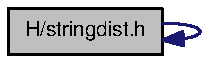
\includegraphics[width=68pt]{stringdist_8h__incl}
\end{center}
\end{figure}
This graph shows which files directly or indirectly include this file:\nopagebreak
\begin{figure}[H]
\begin{center}
\leavevmode
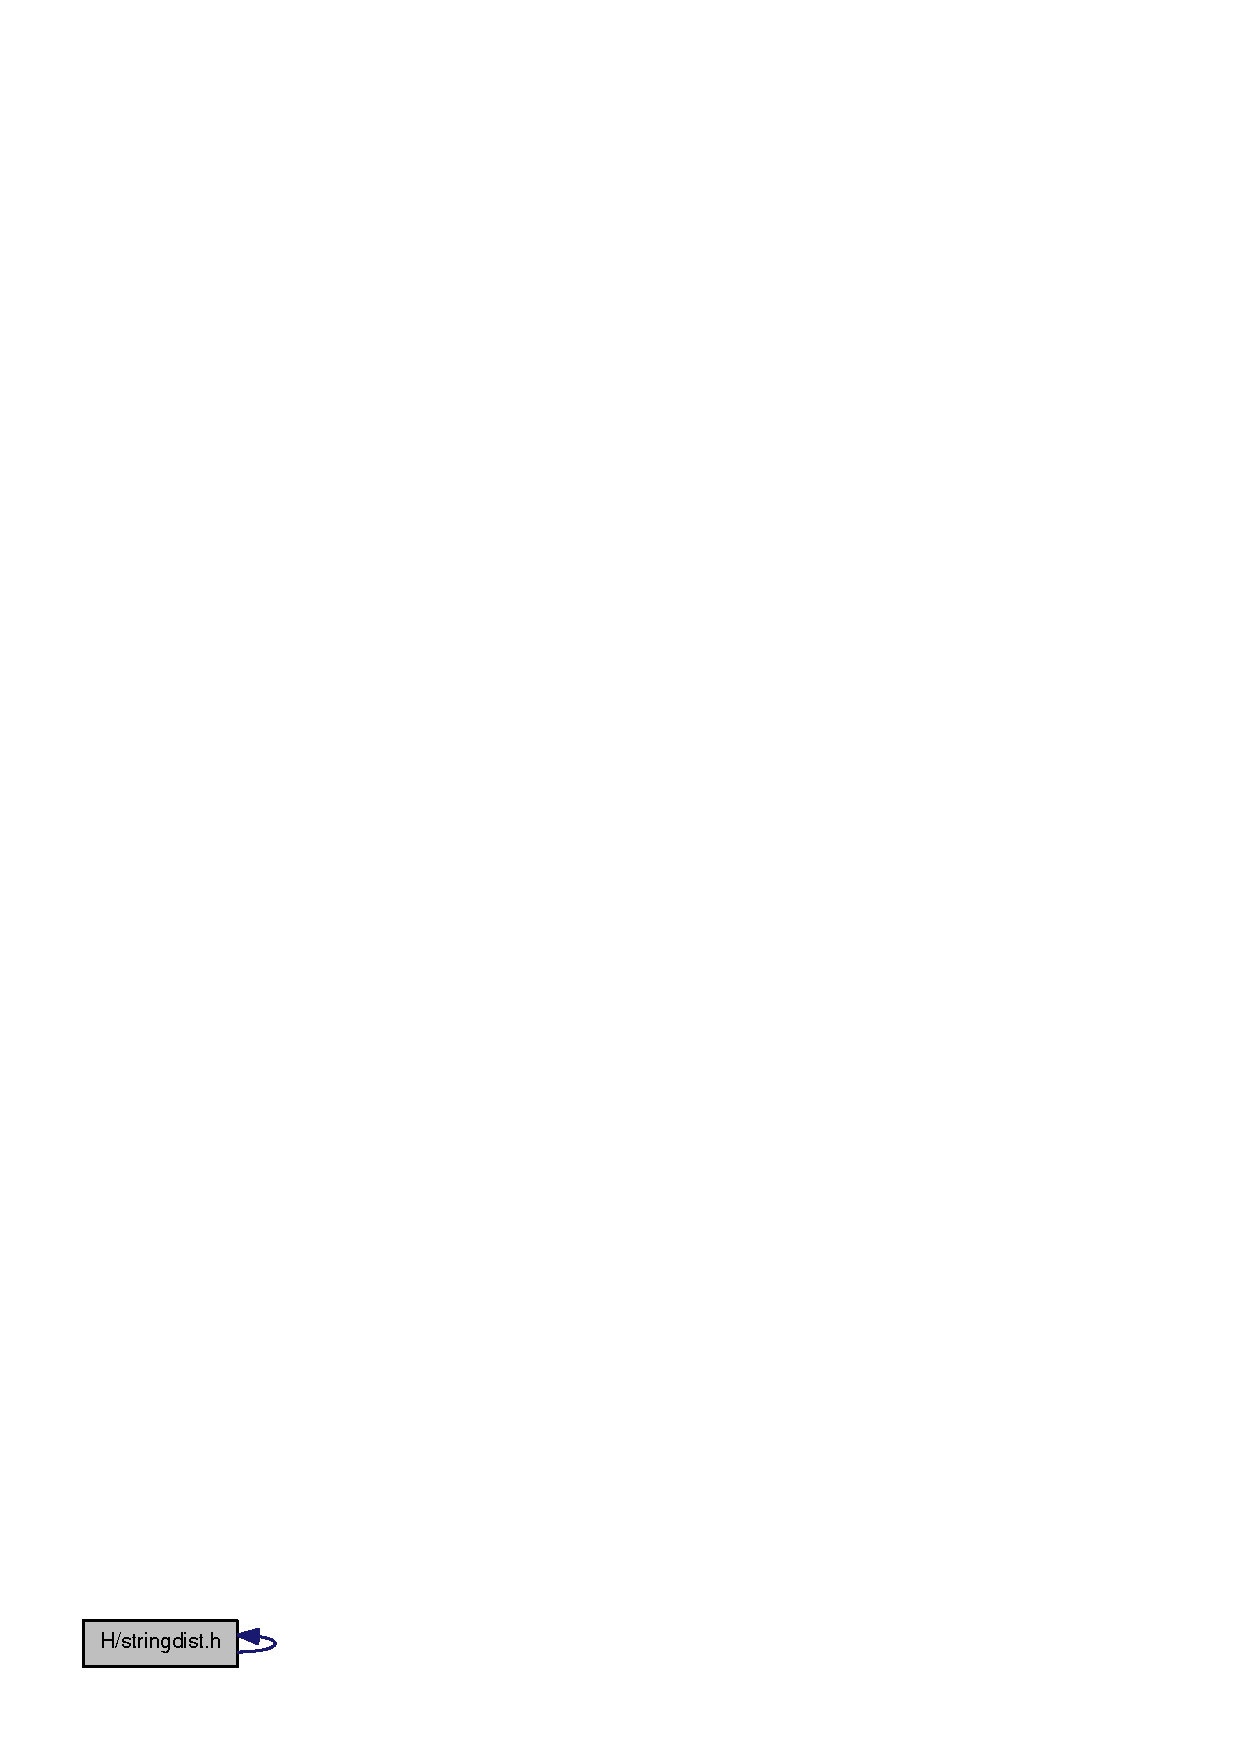
\includegraphics[width=68pt]{stringdist_8h__dep__incl}
\end{center}
\end{figure}
\subsection*{Functions}
\begin{DoxyCompactItemize}
\item 
\hyperlink{structswString}{swString} $\ast$ \hyperlink{stringdist_8h_a3125991b3a403b3f89230474deb3f22e}{Make\_\-swString} (char $\ast$string)
\begin{DoxyCompactList}\small\item\em Convert a structure into a format suitable for \hyperlink{stringdist_8h_a89e3c335ef17780576d7c0e713830db9}{string\_\-edit\_\-distance()}. \item\end{DoxyCompactList}\item 
float \hyperlink{stringdist_8h_a89e3c335ef17780576d7c0e713830db9}{string\_\-edit\_\-distance} (\hyperlink{structswString}{swString} $\ast$T1, \hyperlink{structswString}{swString} $\ast$T2)
\begin{DoxyCompactList}\small\item\em Calculate the string edit distance of T1 and T2. \item\end{DoxyCompactList}\end{DoxyCompactItemize}


\subsection{Detailed Description}
Functions for String Alignment. 

\subsection{Function Documentation}
\hypertarget{stringdist_8h_a3125991b3a403b3f89230474deb3f22e}{
\index{stringdist.h@{stringdist.h}!Make\_\-swString@{Make\_\-swString}}
\index{Make\_\-swString@{Make\_\-swString}!stringdist.h@{stringdist.h}}
\subsubsection[{Make\_\-swString}]{\setlength{\rightskip}{0pt plus 5cm}{\bf swString}$\ast$ Make\_\-swString (char $\ast$ {\em string})}}
\label{stringdist_8h_a3125991b3a403b3f89230474deb3f22e}


Convert a structure into a format suitable for \hyperlink{stringdist_8h_a89e3c335ef17780576d7c0e713830db9}{string\_\-edit\_\-distance()}. 


\begin{DoxyParams}{Parameters}
\item[{\em string}]\begin{DoxyReturn}{Returns}

\end{DoxyReturn}
\end{DoxyParams}
\hypertarget{stringdist_8h_a89e3c335ef17780576d7c0e713830db9}{
\index{stringdist.h@{stringdist.h}!string\_\-edit\_\-distance@{string\_\-edit\_\-distance}}
\index{string\_\-edit\_\-distance@{string\_\-edit\_\-distance}!stringdist.h@{stringdist.h}}
\subsubsection[{string\_\-edit\_\-distance}]{\setlength{\rightskip}{0pt plus 5cm}float string\_\-edit\_\-distance ({\bf swString} $\ast$ {\em T1}, \/  {\bf swString} $\ast$ {\em T2})}}
\label{stringdist_8h_a89e3c335ef17780576d7c0e713830db9}


Calculate the string edit distance of T1 and T2. 


\begin{DoxyParams}{Parameters}
\item[{\em T1}]
\begin{DoxyParams}{Parameters}
\item[{\em T2}]\begin{DoxyReturn}{Returns}

\end{DoxyReturn}
\end{DoxyParams}
\end{DoxyParams}

\hypertarget{subopt_8h}{
\section{H/subopt.h File Reference}
\label{subopt_8h}\index{H/subopt.h@{H/subopt.h}}
}


RNAsubopt and density of states declarations.  


Include dependency graph for subopt.h:\nopagebreak
\begin{figure}[H]
\begin{center}
\leavevmode
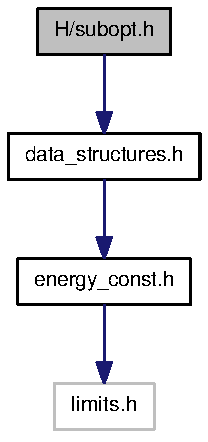
\includegraphics[width=68pt]{subopt_8h__incl}
\end{center}
\end{figure}
\subsection*{Functions}
\begin{DoxyCompactItemize}
\item 
\hyperlink{structSOLUTION}{SOLUTION} $\ast$ \hyperlink{subopt_8h_ac7f749cb177da547798509ebe021884c}{subopt} (char $\ast$seq, char $\ast$sequence, int delta, FILE $\ast$fp)
\begin{DoxyCompactList}\small\item\em Returns list of subopt structures or writes to fp. \item\end{DoxyCompactList}\item 
\hyperlink{structSOLUTION}{SOLUTION} $\ast$ \hyperlink{subopt_8h_a8634516e4740e0b6c9a46d2bae940340}{subopt\_\-circ} (char $\ast$seq, char $\ast$sequence, int delta, FILE $\ast$fp)
\begin{DoxyCompactList}\small\item\em Returns list of circular subopt structures or writes to fp. \item\end{DoxyCompactList}\end{DoxyCompactItemize}
\subsection*{Variables}
\begin{DoxyCompactItemize}
\item 
\hypertarget{subopt_8h_a873cf8ed69e0437f8efa8b1fec854a0e}{
int \hyperlink{subopt_8h_a873cf8ed69e0437f8efa8b1fec854a0e}{subopt\_\-sorted}}
\label{subopt_8h_a873cf8ed69e0437f8efa8b1fec854a0e}

\begin{DoxyCompactList}\small\item\em Sort output by energy. \item\end{DoxyCompactList}\item 
\hypertarget{subopt_8h_a5e57d914bcb5feeecdf520e25313fcfe}{
double \hyperlink{subopt_8h_a5e57d914bcb5feeecdf520e25313fcfe}{print\_\-energy}}
\label{subopt_8h_a5e57d914bcb5feeecdf520e25313fcfe}

\begin{DoxyCompactList}\small\item\em printing threshold for use with logML \item\end{DoxyCompactList}\end{DoxyCompactItemize}


\subsection{Detailed Description}
RNAsubopt and density of states declarations. 

\subsection{Function Documentation}
\hypertarget{subopt_8h_ac7f749cb177da547798509ebe021884c}{
\index{subopt.h@{subopt.h}!subopt@{subopt}}
\index{subopt@{subopt}!subopt.h@{subopt.h}}
\subsubsection[{subopt}]{\setlength{\rightskip}{0pt plus 5cm}{\bf SOLUTION}$\ast$ subopt (char $\ast$ {\em seq}, \/  char $\ast$ {\em sequence}, \/  int {\em delta}, \/  FILE $\ast$ {\em fp})}}
\label{subopt_8h_ac7f749cb177da547798509ebe021884c}


Returns list of subopt structures or writes to fp. 

This function produces {\bfseries all} suboptimal secondary structures within 'delta' $\ast$ 0.01 kcal/mol of the optimum. The results are either directly written to a 'fp' (if 'fp' is not NULL), or (fp==NULL) returned in a \hyperlink{structSOLUTION}{SOLUTION} $\ast$ list terminated by an entry were the 'structure' pointer is NULL.


\begin{DoxyParams}{Parameters}
\item[{\em seq}]
\begin{DoxyParams}{Parameters}
\item[{\em sequence}]
\begin{DoxyParams}{Parameters}
\item[{\em delta}]
\begin{DoxyParams}{Parameters}
\item[{\em fp}]\begin{DoxyReturn}{Returns}

\end{DoxyReturn}
\end{DoxyParams}
\end{DoxyParams}
\end{DoxyParams}
\end{DoxyParams}
\hypertarget{subopt_8h_a8634516e4740e0b6c9a46d2bae940340}{
\index{subopt.h@{subopt.h}!subopt\_\-circ@{subopt\_\-circ}}
\index{subopt\_\-circ@{subopt\_\-circ}!subopt.h@{subopt.h}}
\subsubsection[{subopt\_\-circ}]{\setlength{\rightskip}{0pt plus 5cm}{\bf SOLUTION}$\ast$ subopt\_\-circ (char $\ast$ {\em seq}, \/  char $\ast$ {\em sequence}, \/  int {\em delta}, \/  FILE $\ast$ {\em fp})}}
\label{subopt_8h_a8634516e4740e0b6c9a46d2bae940340}


Returns list of circular subopt structures or writes to fp. 

This function is similar to \hyperlink{subopt_8h_ac7f749cb177da547798509ebe021884c}{subopt()} but calculates secondary structures assuming the RNA sequence to be circular instead of linear


\begin{DoxyParams}{Parameters}
\item[{\em seq}]
\begin{DoxyParams}{Parameters}
\item[{\em sequence}]
\begin{DoxyParams}{Parameters}
\item[{\em delta}]
\begin{DoxyParams}{Parameters}
\item[{\em fp}]\begin{DoxyReturn}{Returns}

\end{DoxyReturn}
\end{DoxyParams}
\end{DoxyParams}
\end{DoxyParams}
\end{DoxyParams}

\hypertarget{treedist_8h}{
\section{H/treedist.h File Reference}
\label{treedist_8h}\index{H/treedist.h@{H/treedist.h}}
}


Functions for \hyperlink{structTree}{Tree} Edit Distances.  


Include dependency graph for treedist.h:\nopagebreak
\begin{figure}[H]
\begin{center}
\leavevmode
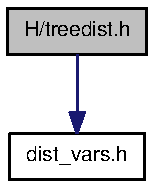
\includegraphics[width=55pt]{treedist_8h__incl}
\end{center}
\end{figure}
\subsection*{Functions}
\begin{DoxyCompactItemize}
\item 
\hyperlink{structTree}{Tree} $\ast$ \hyperlink{treedist_8h_a08fe4d5afd385dce593b86eaf010c6e3}{make\_\-tree} (char $\ast$struc)
\begin{DoxyCompactList}\small\item\em Constructs a \hyperlink{structTree}{Tree} ( essentially the postorder list ) of the structure 'struc', for use in \hyperlink{treedist_8h_a3b21f1925f7071f46d93431a835217bb}{tree\_\-edit\_\-distance()}. \item\end{DoxyCompactList}\item 
float \hyperlink{treedist_8h_a3b21f1925f7071f46d93431a835217bb}{tree\_\-edit\_\-distance} (\hyperlink{structTree}{Tree} $\ast$T1, \hyperlink{structTree}{Tree} $\ast$T2)
\begin{DoxyCompactList}\small\item\em Calculates the edit distance of the two trees. \item\end{DoxyCompactList}\item 
\hypertarget{treedist_8h_a21ad4de3ba4055aeef08b28c9ad48894}{
void \hyperlink{treedist_8h_a21ad4de3ba4055aeef08b28c9ad48894}{print\_\-tree} (\hyperlink{structTree}{Tree} $\ast$t)}
\label{treedist_8h_a21ad4de3ba4055aeef08b28c9ad48894}

\begin{DoxyCompactList}\small\item\em Print a tree (mainly for debugging). \item\end{DoxyCompactList}\item 
void \hyperlink{treedist_8h_acbc1cb9bce582ea945e4a467c76a57aa}{free\_\-tree} (\hyperlink{structTree}{Tree} $\ast$t)
\begin{DoxyCompactList}\small\item\em Free the memory allocated for \hyperlink{structTree}{Tree} t. \item\end{DoxyCompactList}\end{DoxyCompactItemize}


\subsection{Detailed Description}
Functions for \hyperlink{structTree}{Tree} Edit Distances. 

\subsection{Function Documentation}
\hypertarget{treedist_8h_a08fe4d5afd385dce593b86eaf010c6e3}{
\index{treedist.h@{treedist.h}!make\_\-tree@{make\_\-tree}}
\index{make\_\-tree@{make\_\-tree}!treedist.h@{treedist.h}}
\subsubsection[{make\_\-tree}]{\setlength{\rightskip}{0pt plus 5cm}{\bf Tree}$\ast$ make\_\-tree (char $\ast$ {\em struc})}}
\label{treedist_8h_a08fe4d5afd385dce593b86eaf010c6e3}


Constructs a \hyperlink{structTree}{Tree} ( essentially the postorder list ) of the structure 'struc', for use in \hyperlink{treedist_8h_a3b21f1925f7071f46d93431a835217bb}{tree\_\-edit\_\-distance()}. 


\begin{DoxyParams}{Parameters}
\item[{\em struc}]may be any rooted structure representation. \begin{DoxyReturn}{Returns}

\end{DoxyReturn}
\end{DoxyParams}
\hypertarget{treedist_8h_a3b21f1925f7071f46d93431a835217bb}{
\index{treedist.h@{treedist.h}!tree\_\-edit\_\-distance@{tree\_\-edit\_\-distance}}
\index{tree\_\-edit\_\-distance@{tree\_\-edit\_\-distance}!treedist.h@{treedist.h}}
\subsubsection[{tree\_\-edit\_\-distance}]{\setlength{\rightskip}{0pt plus 5cm}float tree\_\-edit\_\-distance ({\bf Tree} $\ast$ {\em T1}, \/  {\bf Tree} $\ast$ {\em T2})}}
\label{treedist_8h_a3b21f1925f7071f46d93431a835217bb}


Calculates the edit distance of the two trees. 


\begin{DoxyParams}{Parameters}
\item[{\em T1}]
\begin{DoxyParams}{Parameters}
\item[{\em T2}]\begin{DoxyReturn}{Returns}

\end{DoxyReturn}
\end{DoxyParams}
\end{DoxyParams}
\hypertarget{treedist_8h_acbc1cb9bce582ea945e4a467c76a57aa}{
\index{treedist.h@{treedist.h}!free\_\-tree@{free\_\-tree}}
\index{free\_\-tree@{free\_\-tree}!treedist.h@{treedist.h}}
\subsubsection[{free\_\-tree}]{\setlength{\rightskip}{0pt plus 5cm}void free\_\-tree ({\bf Tree} $\ast$ {\em t})}}
\label{treedist_8h_acbc1cb9bce582ea945e4a467c76a57aa}


Free the memory allocated for \hyperlink{structTree}{Tree} t. 


\begin{DoxyParams}{Parameters}
\item[{\em t}]\end{DoxyParams}

\hypertarget{utils_8h}{
\section{H/utils.h File Reference}
\label{utils_8h}\index{H/utils.h@{H/utils.h}}
}


Various utility-\/ and helper-\/functions used throughout the Vienna RNA package.  


\subsection*{Defines}
\begin{DoxyCompactItemize}
\item 
\hypertarget{utils_8h_ad403c9ea58f1836689404c2931419c8c}{
\#define \hyperlink{utils_8h_ad403c9ea58f1836689404c2931419c8c}{VRNA\_\-INPUT\_\-ERROR}~1U}
\label{utils_8h_ad403c9ea58f1836689404c2931419c8c}

\begin{DoxyCompactList}\small\item\em Output flag of \hyperlink{utils_8h_a8ef1835eb83f542396f59f0b205965e5}{get\_\-input\_\-line()}: \char`\"{}An ERROR has occured, maybe EOF\char`\"{}. \item\end{DoxyCompactList}\item 
\hypertarget{utils_8h_a72f3c6ca5c83d2b9baed2922d19c403d}{
\#define \hyperlink{utils_8h_a72f3c6ca5c83d2b9baed2922d19c403d}{VRNA\_\-INPUT\_\-QUIT}~2U}
\label{utils_8h_a72f3c6ca5c83d2b9baed2922d19c403d}

\begin{DoxyCompactList}\small\item\em Output flag of \hyperlink{utils_8h_a8ef1835eb83f542396f59f0b205965e5}{get\_\-input\_\-line()}: \char`\"{}the user requested quitting the program\char`\"{}. \item\end{DoxyCompactList}\item 
\hypertarget{utils_8h_a8e3241b321c9c1a78a69e59e2e019a71}{
\#define \hyperlink{utils_8h_a8e3241b321c9c1a78a69e59e2e019a71}{VRNA\_\-INPUT\_\-MISC}~4U}
\label{utils_8h_a8e3241b321c9c1a78a69e59e2e019a71}

\begin{DoxyCompactList}\small\item\em Output flag of \hyperlink{utils_8h_a8ef1835eb83f542396f59f0b205965e5}{get\_\-input\_\-line()}: \char`\"{}something was read\char`\"{}. \item\end{DoxyCompactList}\item 
\#define \hyperlink{utils_8h_a2f0d8069e93d3ac54d9320d6bdb8e7e7}{VRNA\_\-INPUT\_\-FASTA\_\-HEADER}~8U
\begin{DoxyCompactList}\small\item\em Input/Output flag of \hyperlink{utils_8h_a8ef1835eb83f542396f59f0b205965e5}{get\_\-input\_\-line()}:\par
 if used as input option this tells \hyperlink{utils_8h_a8ef1835eb83f542396f59f0b205965e5}{get\_\-input\_\-line()} that the data to be read should comply with the FASTA format. \item\end{DoxyCompactList}\item 
\#define \hyperlink{utils_8h_a8566d6787972100e68b5a2a159b4cf45}{VRNA\_\-INPUT\_\-SEQUENCE}~16U
\begin{DoxyCompactList}\small\item\em Input flag for \hyperlink{utils_8h_a8ef1835eb83f542396f59f0b205965e5}{get\_\-input\_\-line()}:\par
 Tell \hyperlink{utils_8h_a8ef1835eb83f542396f59f0b205965e5}{get\_\-input\_\-line()} that we assume to read a nucleotide sequence. \item\end{DoxyCompactList}\item 
\#define \hyperlink{utils_8h_ac08a9df45b9721b97a47dbfe7a6e5f85}{VRNA\_\-INPUT\_\-CONSTRAINT}~32U
\begin{DoxyCompactList}\small\item\em Input flag for \hyperlink{utils_8h_a8ef1835eb83f542396f59f0b205965e5}{get\_\-input\_\-line()}:\par
 Tell \hyperlink{utils_8h_a8ef1835eb83f542396f59f0b205965e5}{get\_\-input\_\-line()} that we assume to read a structure constraint. \item\end{DoxyCompactList}\item 
\hypertarget{utils_8h_a086742158293217a46ae2f71bb296937}{
\#define \hyperlink{utils_8h_a086742158293217a46ae2f71bb296937}{VRNA\_\-INPUT\_\-NO\_\-TRUNCATION}~256U}
\label{utils_8h_a086742158293217a46ae2f71bb296937}

\begin{DoxyCompactList}\small\item\em Input switch for \hyperlink{utils_8h_a8ef1835eb83f542396f59f0b205965e5}{get\_\-input\_\-line()}: \char`\"{}do not trunkate the line by eliminating white spaces at end of line\char`\"{}. \item\end{DoxyCompactList}\item 
\hypertarget{utils_8h_a7a2e8c50a0c7ce82e60da1016e1367fd}{
\#define \hyperlink{utils_8h_a7a2e8c50a0c7ce82e60da1016e1367fd}{VRNA\_\-INPUT\_\-NO\_\-REST}~512U}
\label{utils_8h_a7a2e8c50a0c7ce82e60da1016e1367fd}

\begin{DoxyCompactList}\small\item\em Input switch for \hyperlink{utils_8h_afd194a69af9d92b5b0412a7627ac1595}{read\_\-record()}: \char`\"{}do fill rest array\char`\"{}. \item\end{DoxyCompactList}\item 
\hypertarget{utils_8h_a0de536599b881c787b0943a2671da476}{
\#define \hyperlink{utils_8h_a0de536599b881c787b0943a2671da476}{VRNA\_\-INPUT\_\-NO\_\-SPAN}~1024U}
\label{utils_8h_a0de536599b881c787b0943a2671da476}

\begin{DoxyCompactList}\small\item\em Input switch for \hyperlink{utils_8h_afd194a69af9d92b5b0412a7627ac1595}{read\_\-record()}: \char`\"{}never allow data to span more than one line\char`\"{}. \item\end{DoxyCompactList}\item 
\hypertarget{utils_8h_ab4db885222b3b69608310d7c7e63e286}{
\#define \hyperlink{utils_8h_ab4db885222b3b69608310d7c7e63e286}{VRNA\_\-INPUT\_\-NOSKIP\_\-BLANK\_\-LINES}~2048U}
\label{utils_8h_ab4db885222b3b69608310d7c7e63e286}

\begin{DoxyCompactList}\small\item\em Input switch for \hyperlink{utils_8h_afd194a69af9d92b5b0412a7627ac1595}{read\_\-record()}: \char`\"{}do not skip empty lines\char`\"{}. \item\end{DoxyCompactList}\item 
\hypertarget{utils_8h_a305474b93ccb79ae4c7754016a8ddd84}{
\#define \hyperlink{utils_8h_a305474b93ccb79ae4c7754016a8ddd84}{VRNA\_\-INPUT\_\-BLANK\_\-LINE}~4096U}
\label{utils_8h_a305474b93ccb79ae4c7754016a8ddd84}

\begin{DoxyCompactList}\small\item\em Output flag for \hyperlink{utils_8h_afd194a69af9d92b5b0412a7627ac1595}{read\_\-record()}: \char`\"{}read an empty line\char`\"{}. \item\end{DoxyCompactList}\item 
\hypertarget{utils_8h_a0f6311f11bed1842e3a527ab27b294c6}{
\#define \hyperlink{utils_8h_a0f6311f11bed1842e3a527ab27b294c6}{VRNA\_\-INPUT\_\-NOSKIP\_\-COMMENTS}~128U}
\label{utils_8h_a0f6311f11bed1842e3a527ab27b294c6}

\begin{DoxyCompactList}\small\item\em Input switch for \hyperlink{utils_8h_a8ef1835eb83f542396f59f0b205965e5}{get\_\-input\_\-line()}: \char`\"{}do not skip comment lines\char`\"{}. \item\end{DoxyCompactList}\item 
\hypertarget{utils_8h_af2062e0eeefffd3ed639af460b3d4fab}{
\#define \hyperlink{utils_8h_af2062e0eeefffd3ed639af460b3d4fab}{VRNA\_\-INPUT\_\-COMMENT}~8192U}
\label{utils_8h_af2062e0eeefffd3ed639af460b3d4fab}

\begin{DoxyCompactList}\small\item\em Output flag for \hyperlink{utils_8h_afd194a69af9d92b5b0412a7627ac1595}{read\_\-record()}: \char`\"{}read a comment\char`\"{}. \item\end{DoxyCompactList}\item 
\hypertarget{utils_8h_a4e8d7120619b21df0309af425acbc9a2}{
\#define \hyperlink{utils_8h_a4e8d7120619b21df0309af425acbc9a2}{VRNA\_\-CONSTRAINT\_\-PIPE}~1U}
\label{utils_8h_a4e8d7120619b21df0309af425acbc9a2}

\begin{DoxyCompactList}\small\item\em pipe sign '$|$' switch for structure constraints (paired with another base) \item\end{DoxyCompactList}\item 
\#define \hyperlink{utils_8h_a55e1d16fd693ae9ec8e987b0750da804}{VRNA\_\-CONSTRAINT\_\-DOT}~2U
\begin{DoxyCompactList}\small\item\em dot '. \item\end{DoxyCompactList}\item 
\hypertarget{utils_8h_a077c56550c915d4516d84a5ed8d051f4}{
\#define \hyperlink{utils_8h_a077c56550c915d4516d84a5ed8d051f4}{VRNA\_\-CONSTRAINT\_\-X}~4U}
\label{utils_8h_a077c56550c915d4516d84a5ed8d051f4}

\begin{DoxyCompactList}\small\item\em 'x' switch for structure constraint (base must not pair) \item\end{DoxyCompactList}\item 
\hypertarget{utils_8h_a0512d790f738742cbdcf3f7c87b46f48}{
\#define \hyperlink{utils_8h_a0512d790f738742cbdcf3f7c87b46f48}{VRNA\_\-CONSTRAINT\_\-ANG\_\-BRACK}~8U}
\label{utils_8h_a0512d790f738742cbdcf3f7c87b46f48}

\begin{DoxyCompactList}\small\item\em angle brackets '$<$', '$>$' switch for structure constraint (paired downstream/upstream) \item\end{DoxyCompactList}\item 
\hypertarget{utils_8h_aa20bfca4bb2903c8548000a33d7bbb53}{
\#define \hyperlink{utils_8h_aa20bfca4bb2903c8548000a33d7bbb53}{VRNA\_\-CONSTRAINT\_\-RND\_\-BRACK}~16U}
\label{utils_8h_aa20bfca4bb2903c8548000a33d7bbb53}

\begin{DoxyCompactList}\small\item\em round brackets '(',')' switch for structure constraint (base i pairs base j) \item\end{DoxyCompactList}\item 
\hypertarget{utils_8h_a7d725ef525b29891abef3f1ed42599a4}{
\#define \hyperlink{utils_8h_a7d725ef525b29891abef3f1ed42599a4}{VRNA\_\-CONSTRAINT\_\-MULTILINE}~32U}
\label{utils_8h_a7d725ef525b29891abef3f1ed42599a4}

\begin{DoxyCompactList}\small\item\em constraint may span over several lines \item\end{DoxyCompactList}\item 
\hypertarget{utils_8h_a08d12a9a846ea593b7171d277c9f033f}{
\#define \hyperlink{utils_8h_a08d12a9a846ea593b7171d277c9f033f}{VRNA\_\-CONSTRAINT\_\-NO\_\-HEADER}~64U}
\label{utils_8h_a08d12a9a846ea593b7171d277c9f033f}

\begin{DoxyCompactList}\small\item\em do not print the header information line \item\end{DoxyCompactList}\item 
\hypertarget{utils_8h_a0a697f77a6fbb10f34e16fa68ed9e655}{
\#define \hyperlink{utils_8h_a0a697f77a6fbb10f34e16fa68ed9e655}{VRNA\_\-CONSTRAINT\_\-ALL}~128U}
\label{utils_8h_a0a697f77a6fbb10f34e16fa68ed9e655}

\begin{DoxyCompactList}\small\item\em placeholder for all constraining characters \item\end{DoxyCompactList}\item 
\hypertarget{utils_8h_ae0b9cd0ce090bd69b951aa73e8fa4f7d}{
\#define \hyperlink{utils_8h_ae0b9cd0ce090bd69b951aa73e8fa4f7d}{MIN2}(A, B)~((A) $<$ (B) ? (A) : (B))}
\label{utils_8h_ae0b9cd0ce090bd69b951aa73e8fa4f7d}

\begin{DoxyCompactList}\small\item\em Get the minimum of two comparable values. \item\end{DoxyCompactList}\item 
\hypertarget{utils_8h_a33297b3679c713b0c4d897cd0fe3b122}{
\#define \hyperlink{utils_8h_a33297b3679c713b0c4d897cd0fe3b122}{MAX2}(A, B)~((A) $>$ (B) ? (A) : (B))}
\label{utils_8h_a33297b3679c713b0c4d897cd0fe3b122}

\begin{DoxyCompactList}\small\item\em Get the maximum of two comparable values. \item\end{DoxyCompactList}\item 
\hypertarget{utils_8h_a721b8d5f3abef17f10293f1f7f8c958e}{
\#define \hyperlink{utils_8h_a721b8d5f3abef17f10293f1f7f8c958e}{MIN3}(A, B, C)~(MIN2(  (MIN2((A),(B))) ,(C)))}
\label{utils_8h_a721b8d5f3abef17f10293f1f7f8c958e}

\begin{DoxyCompactList}\small\item\em Get the minimum of three comparable values. \item\end{DoxyCompactList}\item 
\hypertarget{utils_8h_a8d577123d2e66d2b7d0bf9af6e172b93}{
\#define \hyperlink{utils_8h_a8d577123d2e66d2b7d0bf9af6e172b93}{MAX3}(A, B, C)~(MAX2(  (MAX2((A),(B))) ,(C)))}
\label{utils_8h_a8d577123d2e66d2b7d0bf9af6e172b93}

\begin{DoxyCompactList}\small\item\em Get the maximum of three comparable values. \item\end{DoxyCompactList}\item 
\hypertarget{utils_8h_a03943706e48069237cd57f2d35ca987e}{
\#define \hyperlink{utils_8h_a03943706e48069237cd57f2d35ca987e}{XSTR}(s)~STR(s)}
\label{utils_8h_a03943706e48069237cd57f2d35ca987e}

\begin{DoxyCompactList}\small\item\em Stringify a macro after expansion. \item\end{DoxyCompactList}\item 
\hypertarget{utils_8h_a6388870e639eee9c0a69446876f1f8cc}{
\#define \hyperlink{utils_8h_a6388870e639eee9c0a69446876f1f8cc}{STR}(s)~\#s}
\label{utils_8h_a6388870e639eee9c0a69446876f1f8cc}

\begin{DoxyCompactList}\small\item\em Stringify a macro argument. \item\end{DoxyCompactList}\item 
\#define \hyperlink{utils_8h_afb228174279df9486a5cb56ac0bc79a3}{FILENAME\_\-MAX\_\-LENGTH}~80
\begin{DoxyCompactList}\small\item\em Maximum length of filenames that are generated by our programs. \item\end{DoxyCompactList}\item 
\#define \hyperlink{utils_8h_a33c3b1826b8e2739f09f111ec719ded5}{FILENAME\_\-ID\_\-LENGTH}~42
\begin{DoxyCompactList}\small\item\em Maximum length of id taken from fasta header for filename generation. \item\end{DoxyCompactList}\end{DoxyCompactItemize}
\subsection*{Functions}
\begin{DoxyCompactItemize}
\item 
void $\ast$ \hyperlink{utils_8h_ad7e1e137b3bf1f7108933d302a7f0177}{space} (unsigned size)
\begin{DoxyCompactList}\small\item\em Allocate space safely. \item\end{DoxyCompactList}\item 
void $\ast$ \hyperlink{utils_8h_a9037ada838835b1b9db41581a021b0c8}{xrealloc} (void $\ast$p, unsigned size)
\begin{DoxyCompactList}\small\item\em Reallocate space safely. \item\end{DoxyCompactList}\item 
void \hyperlink{utils_8h_a127ce946e56b5a5773781cabe68e38c5}{nrerror} (const char message\mbox{[}$\,$\mbox{]})
\begin{DoxyCompactList}\small\item\em Die with an error message. \item\end{DoxyCompactList}\item 
void \hyperlink{utils_8h_af2355fa8746f2f30fbe71db65dea3d51}{warn\_\-user} (const char message\mbox{[}$\,$\mbox{]})
\begin{DoxyCompactList}\small\item\em Print a warning message. \item\end{DoxyCompactList}\item 
\hypertarget{utils_8h_a8aaa6d9be6f803f496d9b97375c371f3}{
void \hyperlink{utils_8h_a8aaa6d9be6f803f496d9b97375c371f3}{init\_\-rand} (void)}
\label{utils_8h_a8aaa6d9be6f803f496d9b97375c371f3}

\begin{DoxyCompactList}\small\item\em Make random number seeds. \item\end{DoxyCompactList}\item 
double \hyperlink{utils_8h_aaa328491c84996e445d027fde9800f2e}{urn} (void)
\begin{DoxyCompactList}\small\item\em get a random number from \mbox{[}0..1\mbox{]} \item\end{DoxyCompactList}\item 
int \hyperlink{utils_8h_a68ff0849d44f62fe491800378a5ffcb4}{int\_\-urn} (int from, int to)
\begin{DoxyCompactList}\small\item\em Generates a pseudo random integer in a specified range. \item\end{DoxyCompactList}\item 
char $\ast$ \hyperlink{utils_8h_a7afeb906cb36e9d77379eabc6907ac46}{time\_\-stamp} (void)
\begin{DoxyCompactList}\small\item\em Get a timestamp. \item\end{DoxyCompactList}\item 
char $\ast$ \hyperlink{utils_8h_a1b95eac365a021572e1c37e5993a89be}{random\_\-string} (int l, const char symbols\mbox{[}$\,$\mbox{]})
\begin{DoxyCompactList}\small\item\em Create a random string using characters from a specified symbol set. \item\end{DoxyCompactList}\item 
int \hyperlink{utils_8h_ad9dc7bfc9aa664dc6698f17ce07fc7e7}{hamming} (const char $\ast$s1, const char $\ast$s2)
\begin{DoxyCompactList}\small\item\em Calculate hamming distance between two sequences. \item\end{DoxyCompactList}\item 
int \hyperlink{utils_8h_a96d3c36717d624514055ce201cab1542}{hamming\_\-bound} (const char $\ast$s1, const char $\ast$s2, int n)
\begin{DoxyCompactList}\small\item\em Calculate hamming distance between two sequences up to a specified length. \item\end{DoxyCompactList}\item 
char $\ast$ \hyperlink{utils_8h_abe51806d14cff0789a8c1df7dbc45b71}{get\_\-line} (FILE $\ast$fp)
\begin{DoxyCompactList}\small\item\em Read a line of arbitrary length from a stream. \item\end{DoxyCompactList}\item 
unsigned int \hyperlink{utils_8h_a8ef1835eb83f542396f59f0b205965e5}{get\_\-input\_\-line} (char $\ast$$\ast$string, unsigned int options)
\begin{DoxyCompactList}\small\item\em Retrieve a line from 'stdin' savely while skipping comment characters and other features This function returns the type of input it has read if recognized. \item\end{DoxyCompactList}\item 
unsigned int \hyperlink{utils_8h_afd194a69af9d92b5b0412a7627ac1595}{read\_\-record} (char $\ast$$\ast$header, char $\ast$$\ast$sequence, char $\ast$$\ast$$\ast$rest, unsigned int options)
\begin{DoxyCompactList}\small\item\em Get a data record from stdin. \item\end{DoxyCompactList}\item 
char $\ast$ \hyperlink{utils_8h_ac6dfa5e22928c087c6e09ff0054a7ced}{pack\_\-structure} (const char $\ast$struc)
\begin{DoxyCompactList}\small\item\em Pack secondary secondary structure, 5:1 compression using base 3 encoding. \item\end{DoxyCompactList}\item 
char $\ast$ \hyperlink{utils_8h_a071c6921efe1eb974f115ee6fefa3c39}{unpack\_\-structure} (const char $\ast$packed)
\begin{DoxyCompactList}\small\item\em Unpack secondary structure previously packed with \hyperlink{utils_8h_ac6dfa5e22928c087c6e09ff0054a7ced}{pack\_\-structure()}. \item\end{DoxyCompactList}\item 
short $\ast$ \hyperlink{utils_8h_a89c32307ee50a0026f4a3131fac0845a}{make\_\-pair\_\-table} (const char $\ast$structure)
\begin{DoxyCompactList}\small\item\em Create a pair table of a secondary structure. \item\end{DoxyCompactList}\item 
short $\ast$ \hyperlink{utils_8h_afeaa6d68eef3a99d0a7aa08aa91c6601}{copy\_\-pair\_\-table} (const short $\ast$pt)
\begin{DoxyCompactList}\small\item\em Get an exact copy of a pair table. \item\end{DoxyCompactList}\item 
short $\ast$ \hyperlink{utils_8h_a3c81b3967056c3888b8472b65fbb16f5}{alimake\_\-pair\_\-table} (const char $\ast$structure)
\begin{DoxyCompactList}\small\item\em Pair table for snoop align. \item\end{DoxyCompactList}\item 
short $\ast$ \hyperlink{utils_8h_a9aa3bf3b4346bb7fb88efc154dd07a79}{make\_\-pair\_\-table\_\-snoop} (const char $\ast$structure)
\begin{DoxyCompactList}\small\item\em returns a newly allocated table, such that: table\mbox{[}i\mbox{]}=j if (i.j) pair or 0 if i is unpaired, table\mbox{[}0\mbox{]} contains the length of the structure. \item\end{DoxyCompactList}\item 
int \hyperlink{utils_8h_a6ebbcd29a754f0e4f1a66d1fd84184db}{bp\_\-distance} (const char $\ast$str1, const char $\ast$str2)
\begin{DoxyCompactList}\small\item\em Compute the \char`\"{}base pair\char`\"{} distance between two secondary structures s1 and s2. \item\end{DoxyCompactList}\item 
void \hyperlink{utils_8h_a6bf778117d31b7fd90db435323f4ef74}{print\_\-tty\_\-input\_\-seq} (void)
\begin{DoxyCompactList}\small\item\em Print a line to {\itshape stdout\/} that asks for an input sequence. \item\end{DoxyCompactList}\item 
void \hyperlink{utils_8h_ae4ef89b662a3e9b5b5f0781d9757aba0}{print\_\-tty\_\-input\_\-seq\_\-str} (const char $\ast$s)
\begin{DoxyCompactList}\small\item\em Print a line with a user defined string and a ruler to stdout. \item\end{DoxyCompactList}\item 
void \hyperlink{utils_8h_ae8ae8a34962b9959be3f6c40f0a80ac1}{print\_\-tty\_\-constraint\_\-full} (void)
\begin{DoxyCompactList}\small\item\em Print structure constraint characters to stdout (full constraint support). \item\end{DoxyCompactList}\item 
void \hyperlink{utils_8h_a4d167deb70bb51723e44374dc981deb2}{print\_\-tty\_\-constraint} (unsigned int option)
\begin{DoxyCompactList}\small\item\em Print structure constraint characters to stdout. \item\end{DoxyCompactList}\item 
void \hyperlink{utils_8h_ad3f18dd83f958f18b2f26ecb99305208}{str\_\-DNA2RNA} (char $\ast$sequence)
\begin{DoxyCompactList}\small\item\em Convert a DNA input sequence to RNA alphabet. \item\end{DoxyCompactList}\item 
void \hyperlink{utils_8h_a17b796b806f96b70382077fb5bc519bb}{str\_\-uppercase} (char $\ast$sequence)
\begin{DoxyCompactList}\small\item\em Convert an input sequence to uppercase. \item\end{DoxyCompactList}\item 
int $\ast$ \hyperlink{utils_8h_a55c0f6b3b07b6adf2ee235ba901fe397}{get\_\-iindx} (unsigned int length)
\begin{DoxyCompactList}\small\item\em Get an index mapper array (iindx) for accessing the energy matrices, e.g. \item\end{DoxyCompactList}\item 
int $\ast$ \hyperlink{utils_8h_a4d9ee1572c1bfcd02d3d3f2db8a6530f}{get\_\-indx} (unsigned int length)
\begin{DoxyCompactList}\small\item\em Get an index mapper array (indx) for accessing the energy matrices, e.g. \item\end{DoxyCompactList}\item 
void \hyperlink{utils_8h_a36c3a6c3218b041f992052767bc74549}{constrain\_\-ptypes} (const char $\ast$constraint, unsigned int length, char $\ast$ptype, int $\ast$BP, int min\_\-loop\_\-size, unsigned int idx\_\-type)
\begin{DoxyCompactList}\small\item\em Insert constraining pair types according to constraint structure string. \item\end{DoxyCompactList}\end{DoxyCompactItemize}
\subsection*{Variables}
\begin{DoxyCompactItemize}
\item 
unsigned short \hyperlink{utils_8h_af9a866c8417afda7368bbac939ab3c47}{xsubi} \mbox{[}3\mbox{]}
\begin{DoxyCompactList}\small\item\em Current 48 bit random number. \item\end{DoxyCompactList}\end{DoxyCompactItemize}


\subsection{Detailed Description}
Various utility-\/ and helper-\/functions used throughout the Vienna RNA package. 

\subsection{Define Documentation}
\hypertarget{utils_8h_a2f0d8069e93d3ac54d9320d6bdb8e7e7}{
\index{utils.h@{utils.h}!VRNA\_\-INPUT\_\-FASTA\_\-HEADER@{VRNA\_\-INPUT\_\-FASTA\_\-HEADER}}
\index{VRNA\_\-INPUT\_\-FASTA\_\-HEADER@{VRNA\_\-INPUT\_\-FASTA\_\-HEADER}!utils.h@{utils.h}}
\subsubsection[{VRNA\_\-INPUT\_\-FASTA\_\-HEADER}]{\setlength{\rightskip}{0pt plus 5cm}\#define VRNA\_\-INPUT\_\-FASTA\_\-HEADER~8U}}
\label{utils_8h_a2f0d8069e93d3ac54d9320d6bdb8e7e7}


Input/Output flag of \hyperlink{utils_8h_a8ef1835eb83f542396f59f0b205965e5}{get\_\-input\_\-line()}:\par
 if used as input option this tells \hyperlink{utils_8h_a8ef1835eb83f542396f59f0b205965e5}{get\_\-input\_\-line()} that the data to be read should comply with the FASTA format. 

the function will return this flag if a fasta header was read \hypertarget{utils_8h_a8566d6787972100e68b5a2a159b4cf45}{
\index{utils.h@{utils.h}!VRNA\_\-INPUT\_\-SEQUENCE@{VRNA\_\-INPUT\_\-SEQUENCE}}
\index{VRNA\_\-INPUT\_\-SEQUENCE@{VRNA\_\-INPUT\_\-SEQUENCE}!utils.h@{utils.h}}
\subsubsection[{VRNA\_\-INPUT\_\-SEQUENCE}]{\setlength{\rightskip}{0pt plus 5cm}\#define VRNA\_\-INPUT\_\-SEQUENCE~16U}}
\label{utils_8h_a8566d6787972100e68b5a2a159b4cf45}


Input flag for \hyperlink{utils_8h_a8ef1835eb83f542396f59f0b205965e5}{get\_\-input\_\-line()}:\par
 Tell \hyperlink{utils_8h_a8ef1835eb83f542396f59f0b205965e5}{get\_\-input\_\-line()} that we assume to read a nucleotide sequence. 

\hypertarget{utils_8h_ac08a9df45b9721b97a47dbfe7a6e5f85}{
\index{utils.h@{utils.h}!VRNA\_\-INPUT\_\-CONSTRAINT@{VRNA\_\-INPUT\_\-CONSTRAINT}}
\index{VRNA\_\-INPUT\_\-CONSTRAINT@{VRNA\_\-INPUT\_\-CONSTRAINT}!utils.h@{utils.h}}
\subsubsection[{VRNA\_\-INPUT\_\-CONSTRAINT}]{\setlength{\rightskip}{0pt plus 5cm}\#define VRNA\_\-INPUT\_\-CONSTRAINT~32U}}
\label{utils_8h_ac08a9df45b9721b97a47dbfe7a6e5f85}


Input flag for \hyperlink{utils_8h_a8ef1835eb83f542396f59f0b205965e5}{get\_\-input\_\-line()}:\par
 Tell \hyperlink{utils_8h_a8ef1835eb83f542396f59f0b205965e5}{get\_\-input\_\-line()} that we assume to read a structure constraint. 

\hypertarget{utils_8h_a55e1d16fd693ae9ec8e987b0750da804}{
\index{utils.h@{utils.h}!VRNA\_\-CONSTRAINT\_\-DOT@{VRNA\_\-CONSTRAINT\_\-DOT}}
\index{VRNA\_\-CONSTRAINT\_\-DOT@{VRNA\_\-CONSTRAINT\_\-DOT}!utils.h@{utils.h}}
\subsubsection[{VRNA\_\-CONSTRAINT\_\-DOT}]{\setlength{\rightskip}{0pt plus 5cm}\#define VRNA\_\-CONSTRAINT\_\-DOT~2U}}
\label{utils_8h_a55e1d16fd693ae9ec8e987b0750da804}


dot '. 

' switch for structure constraints (no constraint at all) \hypertarget{utils_8h_afb228174279df9486a5cb56ac0bc79a3}{
\index{utils.h@{utils.h}!FILENAME\_\-MAX\_\-LENGTH@{FILENAME\_\-MAX\_\-LENGTH}}
\index{FILENAME\_\-MAX\_\-LENGTH@{FILENAME\_\-MAX\_\-LENGTH}!utils.h@{utils.h}}
\subsubsection[{FILENAME\_\-MAX\_\-LENGTH}]{\setlength{\rightskip}{0pt plus 5cm}\#define FILENAME\_\-MAX\_\-LENGTH~80}}
\label{utils_8h_afb228174279df9486a5cb56ac0bc79a3}


Maximum length of filenames that are generated by our programs. 

This definition should be used throughout the complete ViennaRNA package wherever a static array holding filenames of output files is declared. \hypertarget{utils_8h_a33c3b1826b8e2739f09f111ec719ded5}{
\index{utils.h@{utils.h}!FILENAME\_\-ID\_\-LENGTH@{FILENAME\_\-ID\_\-LENGTH}}
\index{FILENAME\_\-ID\_\-LENGTH@{FILENAME\_\-ID\_\-LENGTH}!utils.h@{utils.h}}
\subsubsection[{FILENAME\_\-ID\_\-LENGTH}]{\setlength{\rightskip}{0pt plus 5cm}\#define FILENAME\_\-ID\_\-LENGTH~42}}
\label{utils_8h_a33c3b1826b8e2739f09f111ec719ded5}


Maximum length of id taken from fasta header for filename generation. 

this has to be smaller than FILENAME\_\-MAX\_\-LENGTH since in most cases, some suffix will be appended to the ID 

\subsection{Function Documentation}
\hypertarget{utils_8h_ad7e1e137b3bf1f7108933d302a7f0177}{
\index{utils.h@{utils.h}!space@{space}}
\index{space@{space}!utils.h@{utils.h}}
\subsubsection[{space}]{\setlength{\rightskip}{0pt plus 5cm}void$\ast$ space (unsigned {\em size})}}
\label{utils_8h_ad7e1e137b3bf1f7108933d302a7f0177}


Allocate space safely. 


\begin{DoxyParams}{Parameters}
\item[{\em size}]The size of the memory to be allocated in bytes \begin{DoxyReturn}{Returns}
A pointer to the allocated memory 
\end{DoxyReturn}
\end{DoxyParams}
\hypertarget{utils_8h_a9037ada838835b1b9db41581a021b0c8}{
\index{utils.h@{utils.h}!xrealloc@{xrealloc}}
\index{xrealloc@{xrealloc}!utils.h@{utils.h}}
\subsubsection[{xrealloc}]{\setlength{\rightskip}{0pt plus 5cm}void$\ast$ xrealloc (void $\ast$ {\em p}, \/  unsigned {\em size})}}
\label{utils_8h_a9037ada838835b1b9db41581a021b0c8}


Reallocate space safely. 


\begin{DoxyParams}{Parameters}
\item[{\em p}]A pointer to the memory region to be reallocated 
\begin{DoxyParams}{Parameters}
\item[{\em size}]The size of the memory to be allocated in bytes \begin{DoxyReturn}{Returns}
A pointer to the newly allocated memory 
\end{DoxyReturn}
\end{DoxyParams}
\end{DoxyParams}
\hypertarget{utils_8h_a127ce946e56b5a5773781cabe68e38c5}{
\index{utils.h@{utils.h}!nrerror@{nrerror}}
\index{nrerror@{nrerror}!utils.h@{utils.h}}
\subsubsection[{nrerror}]{\setlength{\rightskip}{0pt plus 5cm}void nrerror (const char {\em message}\mbox{[}$\,$\mbox{]})}}
\label{utils_8h_a127ce946e56b5a5773781cabe68e38c5}


Die with an error message. 

\begin{DoxySeeAlso}{See also}
\hyperlink{utils_8h_af2355fa8746f2f30fbe71db65dea3d51}{warn\_\-user()} 
\end{DoxySeeAlso}

\begin{DoxyParams}{Parameters}
\item[{\em message}]The error message to be printed before exiting with 'FAILURE' \end{DoxyParams}
\hypertarget{utils_8h_af2355fa8746f2f30fbe71db65dea3d51}{
\index{utils.h@{utils.h}!warn\_\-user@{warn\_\-user}}
\index{warn\_\-user@{warn\_\-user}!utils.h@{utils.h}}
\subsubsection[{warn\_\-user}]{\setlength{\rightskip}{0pt plus 5cm}void warn\_\-user (const char {\em message}\mbox{[}$\,$\mbox{]})}}
\label{utils_8h_af2355fa8746f2f30fbe71db65dea3d51}


Print a warning message. 

Print a warning message to {\itshape stderr\/} 


\begin{DoxyParams}{Parameters}
\item[{\em message}]The warning message \end{DoxyParams}
\hypertarget{utils_8h_aaa328491c84996e445d027fde9800f2e}{
\index{utils.h@{utils.h}!urn@{urn}}
\index{urn@{urn}!utils.h@{utils.h}}
\subsubsection[{urn}]{\setlength{\rightskip}{0pt plus 5cm}double urn (void)}}
\label{utils_8h_aaa328491c84996e445d027fde9800f2e}


get a random number from \mbox{[}0..1\mbox{]} 

\begin{DoxyNote}{Note}
Usually implemented by calling {\itshape erand48()\/}. 
\end{DoxyNote}
\begin{DoxyReturn}{Returns}
A random number in range \mbox{[}0..1\mbox{]} 
\end{DoxyReturn}
\hypertarget{utils_8h_a68ff0849d44f62fe491800378a5ffcb4}{
\index{utils.h@{utils.h}!int\_\-urn@{int\_\-urn}}
\index{int\_\-urn@{int\_\-urn}!utils.h@{utils.h}}
\subsubsection[{int\_\-urn}]{\setlength{\rightskip}{0pt plus 5cm}int int\_\-urn (int {\em from}, \/  int {\em to})}}
\label{utils_8h_a68ff0849d44f62fe491800378a5ffcb4}


Generates a pseudo random integer in a specified range. 


\begin{DoxyParams}{Parameters}
\item[{\em from}]The first number in range 
\begin{DoxyParams}{Parameters}
\item[{\em to}]The last number in range \begin{DoxyReturn}{Returns}
A pseudo random number in range \mbox{[}from, to\mbox{]} 
\end{DoxyReturn}
\end{DoxyParams}
\end{DoxyParams}
\hypertarget{utils_8h_a7afeb906cb36e9d77379eabc6907ac46}{
\index{utils.h@{utils.h}!time\_\-stamp@{time\_\-stamp}}
\index{time\_\-stamp@{time\_\-stamp}!utils.h@{utils.h}}
\subsubsection[{time\_\-stamp}]{\setlength{\rightskip}{0pt plus 5cm}char$\ast$ time\_\-stamp (void)}}
\label{utils_8h_a7afeb906cb36e9d77379eabc6907ac46}


Get a timestamp. 

Returns a string containing the current date in the format \begin{DoxyVerb}Fri Mar 19 21:10:57 1993\end{DoxyVerb}


\begin{DoxyReturn}{Returns}
A string containing the timestamp 
\end{DoxyReturn}
\hypertarget{utils_8h_a1b95eac365a021572e1c37e5993a89be}{
\index{utils.h@{utils.h}!random\_\-string@{random\_\-string}}
\index{random\_\-string@{random\_\-string}!utils.h@{utils.h}}
\subsubsection[{random\_\-string}]{\setlength{\rightskip}{0pt plus 5cm}char$\ast$ random\_\-string (int {\em l}, \/  const char {\em symbols}\mbox{[}$\,$\mbox{]})}}
\label{utils_8h_a1b95eac365a021572e1c37e5993a89be}


Create a random string using characters from a specified symbol set. 


\begin{DoxyParams}{Parameters}
\item[{\em l}]The length of the sequence 
\begin{DoxyParams}{Parameters}
\item[{\em symbols}]The symbol set \begin{DoxyReturn}{Returns}
A random string of length 'l' containing characters from the symbolset 
\end{DoxyReturn}
\end{DoxyParams}
\end{DoxyParams}
\hypertarget{utils_8h_ad9dc7bfc9aa664dc6698f17ce07fc7e7}{
\index{utils.h@{utils.h}!hamming@{hamming}}
\index{hamming@{hamming}!utils.h@{utils.h}}
\subsubsection[{hamming}]{\setlength{\rightskip}{0pt plus 5cm}int hamming (const char $\ast$ {\em s1}, \/  const char $\ast$ {\em s2})}}
\label{utils_8h_ad9dc7bfc9aa664dc6698f17ce07fc7e7}


Calculate hamming distance between two sequences. 

Calculate the number of positions in which 
\begin{DoxyParams}{Parameters}
\item[{\em s1}]The first sequence 
\begin{DoxyParams}{Parameters}
\item[{\em s2}]The second sequence \begin{DoxyReturn}{Returns}
The hamming distance between s1 and s2 
\end{DoxyReturn}
\end{DoxyParams}
\end{DoxyParams}
\hypertarget{utils_8h_a96d3c36717d624514055ce201cab1542}{
\index{utils.h@{utils.h}!hamming\_\-bound@{hamming\_\-bound}}
\index{hamming\_\-bound@{hamming\_\-bound}!utils.h@{utils.h}}
\subsubsection[{hamming\_\-bound}]{\setlength{\rightskip}{0pt plus 5cm}int hamming\_\-bound (const char $\ast$ {\em s1}, \/  const char $\ast$ {\em s2}, \/  int {\em n})}}
\label{utils_8h_a96d3c36717d624514055ce201cab1542}


Calculate hamming distance between two sequences up to a specified length. 

This function is similar to \hyperlink{utils_8h_ad9dc7bfc9aa664dc6698f17ce07fc7e7}{hamming()} but instead of comparing both sequences up to their actual length only the first 'n' characters are taken into account 
\begin{DoxyParams}{Parameters}
\item[{\em s1}]The first sequence 
\begin{DoxyParams}{Parameters}
\item[{\em s2}]The second sequence \begin{DoxyReturn}{Returns}
The hamming distance between s1 and s2 
\end{DoxyReturn}
\end{DoxyParams}
\end{DoxyParams}
\hypertarget{utils_8h_abe51806d14cff0789a8c1df7dbc45b71}{
\index{utils.h@{utils.h}!get\_\-line@{get\_\-line}}
\index{get\_\-line@{get\_\-line}!utils.h@{utils.h}}
\subsubsection[{get\_\-line}]{\setlength{\rightskip}{0pt plus 5cm}char$\ast$ get\_\-line (FILE $\ast$ {\em fp})}}
\label{utils_8h_abe51806d14cff0789a8c1df7dbc45b71}


Read a line of arbitrary length from a stream. 

Returns a pointer to the resulting string. The necessary memory is allocated and should be released using {\itshape free()\/} when the string is no longer needed.


\begin{DoxyParams}{Parameters}
\item[{\em fp}]A file pointer to the stream where the function should read from \begin{DoxyReturn}{Returns}
A pointer to the resulting string 
\end{DoxyReturn}
\end{DoxyParams}
\hypertarget{utils_8h_a8ef1835eb83f542396f59f0b205965e5}{
\index{utils.h@{utils.h}!get\_\-input\_\-line@{get\_\-input\_\-line}}
\index{get\_\-input\_\-line@{get\_\-input\_\-line}!utils.h@{utils.h}}
\subsubsection[{get\_\-input\_\-line}]{\setlength{\rightskip}{0pt plus 5cm}unsigned int get\_\-input\_\-line (char $\ast$$\ast$ {\em string}, \/  unsigned int {\em options})}}
\label{utils_8h_a8ef1835eb83f542396f59f0b205965e5}


Retrieve a line from 'stdin' savely while skipping comment characters and other features This function returns the type of input it has read if recognized. 

An option argument allows to switch between different reading modes.\par
 Currently available options are:\par
 VRNA\_\-INPUT\_\-NOPRINT\_\-COMMENTS, \hyperlink{utils_8h_a0f6311f11bed1842e3a527ab27b294c6}{VRNA\_\-INPUT\_\-NOSKIP\_\-COMMENTS}, VRNA\_\-INPUT\_\-NOELIM\_\-WS\_\-SUFFIX

pass a collection of options as one value like this: \begin{DoxyVerb}get_input_line(string, option_1 | option_2 | option_n) \end{DoxyVerb}


If the function recognizes the type of input, it will report it in the return value. It also reports if a user defined 'quit' command (@-\/sign on 'stdin') was given. Possible return values are:\par
 \hyperlink{utils_8h_a2f0d8069e93d3ac54d9320d6bdb8e7e7}{VRNA\_\-INPUT\_\-FASTA\_\-HEADER}, \hyperlink{utils_8h_ad403c9ea58f1836689404c2931419c8c}{VRNA\_\-INPUT\_\-ERROR}, \hyperlink{utils_8h_a8e3241b321c9c1a78a69e59e2e019a71}{VRNA\_\-INPUT\_\-MISC}, \hyperlink{utils_8h_a72f3c6ca5c83d2b9baed2922d19c403d}{VRNA\_\-INPUT\_\-QUIT}


\begin{DoxyParams}{Parameters}
\item[{\em string}]A pointer to the character array that contains the line read 
\begin{DoxyParams}{Parameters}
\item[{\em options}]A collection of options for switching the functions behavior \begin{DoxyReturn}{Returns}
A flag with information about what has been read 
\end{DoxyReturn}
\end{DoxyParams}
\end{DoxyParams}
\hypertarget{utils_8h_afd194a69af9d92b5b0412a7627ac1595}{
\index{utils.h@{utils.h}!read\_\-record@{read\_\-record}}
\index{read\_\-record@{read\_\-record}!utils.h@{utils.h}}
\subsubsection[{read\_\-record}]{\setlength{\rightskip}{0pt plus 5cm}unsigned int read\_\-record (char $\ast$$\ast$ {\em header}, \/  char $\ast$$\ast$ {\em sequence}, \/  char $\ast$$\ast$$\ast$ {\em rest}, \/  unsigned int {\em options})}}
\label{utils_8h_afd194a69af9d92b5b0412a7627ac1595}


Get a data record from stdin. 

This function may be used to obtain complete datasets from stdin. A dataset is always defined to contain at least a sequence. If data on stdin starts with a fasta header, i.e. a line like \begin{DoxyVerb}>some header info \end{DoxyVerb}
 then \hyperlink{utils_8h_afd194a69af9d92b5b0412a7627ac1595}{read\_\-record()} will assume that the sequence that follows the header may span over several lines. To disable this behavior and to assign a single line to the argument 'sequence' one can pass VRNA\_\-INPUT\_\-NO\_\-SPAN in the 'options' argument. If no fasta header is read in the beginning of a data block, a sequence must not span over multiple lines!\par
 Unless the options \hyperlink{utils_8h_a0f6311f11bed1842e3a527ab27b294c6}{VRNA\_\-INPUT\_\-NOSKIP\_\-COMMENTS} or \hyperlink{utils_8h_ab4db885222b3b69608310d7c7e63e286}{VRNA\_\-INPUT\_\-NOSKIP\_\-BLANK\_\-LINES} are passed, a sequence may be interrupted by lines starting with a comment character or empty lines.\par
 A sequence is regarded as completely read if it was either assumed to not span over multiple lines, a secondary structure or structure constraint follows the sequence on the next line or a new header marks the beginning of a new sequence...\par
 All lines following the sequence (this includes comments) and not initiating a new dataset are available through the line-\/array 'rest'. Here one can usually find the structure constraint or other information belonging to the current dataset. Filling of 'rest' may be prevented by passing \hyperlink{utils_8h_a7a2e8c50a0c7ce82e60da1016e1367fd}{VRNA\_\-INPUT\_\-NO\_\-REST} to the options argument.\par


\begin{DoxyNote}{Note}
This function will exit any program with an error message if no sequence could be read!
\end{DoxyNote}
The main purpose of this function is to be able to easily parse blocks of data from stdin in the header of a loop where all calculations for the appropriate data is done inside the loop. The loop may be then left on certain return values, e.g.: \begin{DoxyVerb}
char *id, *seq, **rest;
int  i;
while(!(read_record(&id, &seq, &rest, 0) & (VRNA_INPUT_ERROR | VRNA_INPUT_QUIT))){
  if(id) printf("%s\n", id);
  printf("%s\n", seq);
  if(rest)
    for(i=0;rest[i];i++)
      printf("%s\n", rest[i]);
} \end{DoxyVerb}


In the example above, the while loop will be terminated when \hyperlink{utils_8h_afd194a69af9d92b5b0412a7627ac1595}{read\_\-record()} returns either an error or a user initiated quit request.\par
 As long as data is read from stdin, the id is printed if it is available for the current block of data. The sequence will be printed in any case and if some more lines belong to the current block of data each line will be printed as well.

\begin{DoxyNote}{Note}
Do not forget to free the memory occupied by header, sequence and rest!
\end{DoxyNote}

\begin{DoxyParams}{Parameters}
\item[{\em header}]A pointer which will be set such that it points to the header of the record 
\begin{DoxyParams}{Parameters}
\item[{\em sequence}]A pointer which will be set such that it points to the sequence of the record 
\begin{DoxyParams}{Parameters}
\item[{\em rest}]A pointer which will be set such that it points to an array of lines which also belong to the record 
\begin{DoxyParams}{Parameters}
\item[{\em options}]Some options which may be passed to alter the behavior of the function, use 0 for no options \begin{DoxyReturn}{Returns}
A flag with information about what the function actually did read 
\end{DoxyReturn}
\end{DoxyParams}
\end{DoxyParams}
\end{DoxyParams}
\end{DoxyParams}
\hypertarget{utils_8h_ac6dfa5e22928c087c6e09ff0054a7ced}{
\index{utils.h@{utils.h}!pack\_\-structure@{pack\_\-structure}}
\index{pack\_\-structure@{pack\_\-structure}!utils.h@{utils.h}}
\subsubsection[{pack\_\-structure}]{\setlength{\rightskip}{0pt plus 5cm}char$\ast$ pack\_\-structure (const char $\ast$ {\em struc})}}
\label{utils_8h_ac6dfa5e22928c087c6e09ff0054a7ced}


Pack secondary secondary structure, 5:1 compression using base 3 encoding. 

Returns a binary string encoding of the secondary structure using a 5:1 compression scheme. The string is NULL terminated and can therefore be used with standard string functions such as strcmp(). Useful for programs that need to keep many structures in memory.


\begin{DoxyParams}{Parameters}
\item[{\em struc}]The secondary structure in dot-\/bracket notation \begin{DoxyReturn}{Returns}
The binary encoded structure 
\end{DoxyReturn}
\end{DoxyParams}
\hypertarget{utils_8h_a071c6921efe1eb974f115ee6fefa3c39}{
\index{utils.h@{utils.h}!unpack\_\-structure@{unpack\_\-structure}}
\index{unpack\_\-structure@{unpack\_\-structure}!utils.h@{utils.h}}
\subsubsection[{unpack\_\-structure}]{\setlength{\rightskip}{0pt plus 5cm}char$\ast$ unpack\_\-structure (const char $\ast$ {\em packed})}}
\label{utils_8h_a071c6921efe1eb974f115ee6fefa3c39}


Unpack secondary structure previously packed with \hyperlink{utils_8h_ac6dfa5e22928c087c6e09ff0054a7ced}{pack\_\-structure()}. 

Translate a compressed binary string produced by \hyperlink{utils_8h_ac6dfa5e22928c087c6e09ff0054a7ced}{pack\_\-structure()} back into the familiar dot-\/bracket notation.


\begin{DoxyParams}{Parameters}
\item[{\em packed}]The binary encoded packed secondary structure \begin{DoxyReturn}{Returns}
The unpacked secondary structure in dot-\/bracket notation 
\end{DoxyReturn}
\end{DoxyParams}
\hypertarget{utils_8h_a89c32307ee50a0026f4a3131fac0845a}{
\index{utils.h@{utils.h}!make\_\-pair\_\-table@{make\_\-pair\_\-table}}
\index{make\_\-pair\_\-table@{make\_\-pair\_\-table}!utils.h@{utils.h}}
\subsubsection[{make\_\-pair\_\-table}]{\setlength{\rightskip}{0pt plus 5cm}short$\ast$ make\_\-pair\_\-table (const char $\ast$ {\em structure})}}
\label{utils_8h_a89c32307ee50a0026f4a3131fac0845a}


Create a pair table of a secondary structure. 

Returns a newly allocated table, such that table\mbox{[}i\mbox{]}=j if (i.j) pair or 0 if i is unpaired, table\mbox{[}0\mbox{]} contains the length of the structure.


\begin{DoxyParams}{Parameters}
\item[{\em structure}]The secondary structure in dot-\/bracket notation \begin{DoxyReturn}{Returns}
A pointer to the created pair\_\-table 
\end{DoxyReturn}
\end{DoxyParams}
\hypertarget{utils_8h_afeaa6d68eef3a99d0a7aa08aa91c6601}{
\index{utils.h@{utils.h}!copy\_\-pair\_\-table@{copy\_\-pair\_\-table}}
\index{copy\_\-pair\_\-table@{copy\_\-pair\_\-table}!utils.h@{utils.h}}
\subsubsection[{copy\_\-pair\_\-table}]{\setlength{\rightskip}{0pt plus 5cm}short$\ast$ copy\_\-pair\_\-table (const short $\ast$ {\em pt})}}
\label{utils_8h_afeaa6d68eef3a99d0a7aa08aa91c6601}


Get an exact copy of a pair table. 


\begin{DoxyParams}{Parameters}
\item[{\em pt}]The pair table to be copied \begin{DoxyReturn}{Returns}
A pointer to the copy of 'pt' 
\end{DoxyReturn}
\end{DoxyParams}
\hypertarget{utils_8h_a3c81b3967056c3888b8472b65fbb16f5}{
\index{utils.h@{utils.h}!alimake\_\-pair\_\-table@{alimake\_\-pair\_\-table}}
\index{alimake\_\-pair\_\-table@{alimake\_\-pair\_\-table}!utils.h@{utils.h}}
\subsubsection[{alimake\_\-pair\_\-table}]{\setlength{\rightskip}{0pt plus 5cm}short$\ast$ alimake\_\-pair\_\-table (const char $\ast$ {\em structure})}}
\label{utils_8h_a3c81b3967056c3888b8472b65fbb16f5}


Pair table for snoop align. 

\hypertarget{utils_8h_a9aa3bf3b4346bb7fb88efc154dd07a79}{
\index{utils.h@{utils.h}!make\_\-pair\_\-table\_\-snoop@{make\_\-pair\_\-table\_\-snoop}}
\index{make\_\-pair\_\-table\_\-snoop@{make\_\-pair\_\-table\_\-snoop}!utils.h@{utils.h}}
\subsubsection[{make\_\-pair\_\-table\_\-snoop}]{\setlength{\rightskip}{0pt plus 5cm}short$\ast$ make\_\-pair\_\-table\_\-snoop (const char $\ast$ {\em structure})}}
\label{utils_8h_a9aa3bf3b4346bb7fb88efc154dd07a79}


returns a newly allocated table, such that: table\mbox{[}i\mbox{]}=j if (i.j) pair or 0 if i is unpaired, table\mbox{[}0\mbox{]} contains the length of the structure. 

The special pseudoknotted H/ACA-\/mRNA structure is taken into account. \hypertarget{utils_8h_a6ebbcd29a754f0e4f1a66d1fd84184db}{
\index{utils.h@{utils.h}!bp\_\-distance@{bp\_\-distance}}
\index{bp\_\-distance@{bp\_\-distance}!utils.h@{utils.h}}
\subsubsection[{bp\_\-distance}]{\setlength{\rightskip}{0pt plus 5cm}int bp\_\-distance (const char $\ast$ {\em str1}, \/  const char $\ast$ {\em str2})}}
\label{utils_8h_a6ebbcd29a754f0e4f1a66d1fd84184db}


Compute the \char`\"{}base pair\char`\"{} distance between two secondary structures s1 and s2. 

The sequences should have the same length. dist = number of base pairs in one structure but not in the other same as edit distance with open-\/pair close-\/pair as move-\/set


\begin{DoxyParams}{Parameters}
\item[{\em str1}]First structure in dot-\/bracket notation 
\begin{DoxyParams}{Parameters}
\item[{\em str2}]Second structure in dot-\/bracket notation \begin{DoxyReturn}{Returns}
The base pair distance between str1 and str2 
\end{DoxyReturn}
\end{DoxyParams}
\end{DoxyParams}
\hypertarget{utils_8h_a6bf778117d31b7fd90db435323f4ef74}{
\index{utils.h@{utils.h}!print\_\-tty\_\-input\_\-seq@{print\_\-tty\_\-input\_\-seq}}
\index{print\_\-tty\_\-input\_\-seq@{print\_\-tty\_\-input\_\-seq}!utils.h@{utils.h}}
\subsubsection[{print\_\-tty\_\-input\_\-seq}]{\setlength{\rightskip}{0pt plus 5cm}void print\_\-tty\_\-input\_\-seq (void)}}
\label{utils_8h_a6bf778117d31b7fd90db435323f4ef74}


Print a line to {\itshape stdout\/} that asks for an input sequence. 

There will also be a ruler (scale line) printed that helps orientation of the sequence positions \hypertarget{utils_8h_ae4ef89b662a3e9b5b5f0781d9757aba0}{
\index{utils.h@{utils.h}!print\_\-tty\_\-input\_\-seq\_\-str@{print\_\-tty\_\-input\_\-seq\_\-str}}
\index{print\_\-tty\_\-input\_\-seq\_\-str@{print\_\-tty\_\-input\_\-seq\_\-str}!utils.h@{utils.h}}
\subsubsection[{print\_\-tty\_\-input\_\-seq\_\-str}]{\setlength{\rightskip}{0pt plus 5cm}void print\_\-tty\_\-input\_\-seq\_\-str (const char $\ast$ {\em s})}}
\label{utils_8h_ae4ef89b662a3e9b5b5f0781d9757aba0}


Print a line with a user defined string and a ruler to stdout. 

(usually this is used to ask for user input) There will also be a ruler (scale line) printed that helps orientation of the sequence positions


\begin{DoxyParams}{Parameters}
\item[{\em s}]A user defined string that will be printed to stdout \end{DoxyParams}
\hypertarget{utils_8h_ae8ae8a34962b9959be3f6c40f0a80ac1}{
\index{utils.h@{utils.h}!print\_\-tty\_\-constraint\_\-full@{print\_\-tty\_\-constraint\_\-full}}
\index{print\_\-tty\_\-constraint\_\-full@{print\_\-tty\_\-constraint\_\-full}!utils.h@{utils.h}}
\subsubsection[{print\_\-tty\_\-constraint\_\-full}]{\setlength{\rightskip}{0pt plus 5cm}void print\_\-tty\_\-constraint\_\-full (void)}}
\label{utils_8h_ae8ae8a34962b9959be3f6c40f0a80ac1}


Print structure constraint characters to stdout (full constraint support). 

\hypertarget{utils_8h_a4d167deb70bb51723e44374dc981deb2}{
\index{utils.h@{utils.h}!print\_\-tty\_\-constraint@{print\_\-tty\_\-constraint}}
\index{print\_\-tty\_\-constraint@{print\_\-tty\_\-constraint}!utils.h@{utils.h}}
\subsubsection[{print\_\-tty\_\-constraint}]{\setlength{\rightskip}{0pt plus 5cm}void print\_\-tty\_\-constraint (unsigned int {\em option})}}
\label{utils_8h_a4d167deb70bb51723e44374dc981deb2}


Print structure constraint characters to stdout. 

(constraint support is specified by option parameter)

Currently available options are:\par
 \hyperlink{utils_8h_a4e8d7120619b21df0309af425acbc9a2}{VRNA\_\-CONSTRAINT\_\-PIPE} (paired with another base)\par
 \hyperlink{utils_8h_a55e1d16fd693ae9ec8e987b0750da804}{VRNA\_\-CONSTRAINT\_\-DOT} (no constraint at all)\par
 \hyperlink{utils_8h_a077c56550c915d4516d84a5ed8d051f4}{VRNA\_\-CONSTRAINT\_\-X} (base must not pair)\par
 \hyperlink{utils_8h_a0512d790f738742cbdcf3f7c87b46f48}{VRNA\_\-CONSTRAINT\_\-ANG\_\-BRACK} (paired downstream/upstream)\par
 \hyperlink{utils_8h_aa20bfca4bb2903c8548000a33d7bbb53}{VRNA\_\-CONSTRAINT\_\-RND\_\-BRACK} (base i pairs base j)\par


pass a collection of options as one value like this: \begin{DoxyVerb}print_tty_constraint(option_1 | option_2 | option_n) \end{DoxyVerb}



\begin{DoxyParams}{Parameters}
\item[{\em option}]Option switch that tells which constraint help will be printed \end{DoxyParams}
\hypertarget{utils_8h_ad3f18dd83f958f18b2f26ecb99305208}{
\index{utils.h@{utils.h}!str\_\-DNA2RNA@{str\_\-DNA2RNA}}
\index{str\_\-DNA2RNA@{str\_\-DNA2RNA}!utils.h@{utils.h}}
\subsubsection[{str\_\-DNA2RNA}]{\setlength{\rightskip}{0pt plus 5cm}void str\_\-DNA2RNA (char $\ast$ {\em sequence})}}
\label{utils_8h_ad3f18dd83f958f18b2f26ecb99305208}


Convert a DNA input sequence to RNA alphabet. 

This function substitudes {\itshape T\/} and {\itshape t\/} with {\itshape U\/} and {\itshape u\/}, respectively


\begin{DoxyParams}{Parameters}
\item[{\em sequence}]The sequence to be converted \end{DoxyParams}
\hypertarget{utils_8h_a17b796b806f96b70382077fb5bc519bb}{
\index{utils.h@{utils.h}!str\_\-uppercase@{str\_\-uppercase}}
\index{str\_\-uppercase@{str\_\-uppercase}!utils.h@{utils.h}}
\subsubsection[{str\_\-uppercase}]{\setlength{\rightskip}{0pt plus 5cm}void str\_\-uppercase (char $\ast$ {\em sequence})}}
\label{utils_8h_a17b796b806f96b70382077fb5bc519bb}


Convert an input sequence to uppercase. 


\begin{DoxyParams}{Parameters}
\item[{\em sequence}]The sequence to be converted \end{DoxyParams}
\hypertarget{utils_8h_a55c0f6b3b07b6adf2ee235ba901fe397}{
\index{utils.h@{utils.h}!get\_\-iindx@{get\_\-iindx}}
\index{get\_\-iindx@{get\_\-iindx}!utils.h@{utils.h}}
\subsubsection[{get\_\-iindx}]{\setlength{\rightskip}{0pt plus 5cm}int$\ast$ get\_\-iindx (unsigned int {\em length})}}
\label{utils_8h_a55c0f6b3b07b6adf2ee235ba901fe397}


Get an index mapper array (iindx) for accessing the energy matrices, e.g. 

in partition function related functions.

Access of a position \char`\"{}(i,j)\char`\"{} is then accomplished by using \begin{DoxyVerb}(i,j) ~ iindx[i]-j \end{DoxyVerb}
 This function is necessary as most of the two-\/dimensional energy matrices are actually one-\/dimensional arrays throughout the ViennaRNAPackage

Consult the implemented code to find out about the mapping formula ;)

\begin{DoxySeeAlso}{See also}
\hyperlink{utils_8h_a4d9ee1572c1bfcd02d3d3f2db8a6530f}{get\_\-indx()} 
\end{DoxySeeAlso}

\begin{DoxyParams}{Parameters}
\item[{\em length}]The length of the RNA sequence \begin{DoxyReturn}{Returns}
The mapper array 
\end{DoxyReturn}
\end{DoxyParams}
\hypertarget{utils_8h_a4d9ee1572c1bfcd02d3d3f2db8a6530f}{
\index{utils.h@{utils.h}!get\_\-indx@{get\_\-indx}}
\index{get\_\-indx@{get\_\-indx}!utils.h@{utils.h}}
\subsubsection[{get\_\-indx}]{\setlength{\rightskip}{0pt plus 5cm}int$\ast$ get\_\-indx (unsigned int {\em length})}}
\label{utils_8h_a4d9ee1572c1bfcd02d3d3f2db8a6530f}


Get an index mapper array (indx) for accessing the energy matrices, e.g. 

in MFE related functions.

Access of a position \char`\"{}(i,j)\char`\"{} is then accomplished by using \begin{DoxyVerb}(i,j) ~ indx[j]+i \end{DoxyVerb}
 This function is necessary as most of the two-\/dimensional energy matrices are actually one-\/dimensional arrays throughout the ViennaRNAPackage

Consult the implemented code to find out about the mapping formula ;)

\begin{DoxySeeAlso}{See also}
\hyperlink{utils_8h_a55c0f6b3b07b6adf2ee235ba901fe397}{get\_\-iindx()} 
\end{DoxySeeAlso}

\begin{DoxyParams}{Parameters}
\item[{\em length}]The length of the RNA sequence \begin{DoxyReturn}{Returns}
The mapper array 
\end{DoxyReturn}
\end{DoxyParams}
\hypertarget{utils_8h_a36c3a6c3218b041f992052767bc74549}{
\index{utils.h@{utils.h}!constrain\_\-ptypes@{constrain\_\-ptypes}}
\index{constrain\_\-ptypes@{constrain\_\-ptypes}!utils.h@{utils.h}}
\subsubsection[{constrain\_\-ptypes}]{\setlength{\rightskip}{0pt plus 5cm}void constrain\_\-ptypes (const char $\ast$ {\em constraint}, \/  unsigned int {\em length}, \/  char $\ast$ {\em ptype}, \/  int $\ast$ {\em BP}, \/  int {\em min\_\-loop\_\-size}, \/  unsigned int {\em idx\_\-type})}}
\label{utils_8h_a36c3a6c3218b041f992052767bc74549}


Insert constraining pair types according to constraint structure string. 

\begin{DoxySeeAlso}{See also}
\hyperlink{utils_8h_a4d9ee1572c1bfcd02d3d3f2db8a6530f}{get\_\-indx()}, \hyperlink{utils_8h_a55c0f6b3b07b6adf2ee235ba901fe397}{get\_\-iindx()}
\end{DoxySeeAlso}

\begin{DoxyParams}{Parameters}
\item[{\em constraint}]The structure constraint string 
\begin{DoxyParams}{Parameters}
\item[{\em length}]The actual length of the sequence (constraint may be shorter) 
\begin{DoxyParams}{Parameters}
\item[{\em ptype}]A pointer to the basepair type array 
\begin{DoxyParams}{Parameters}
\item[{\em min\_\-loop\_\-size}]The minimal loop size (usually \hyperlink{energy__const_8h_ae646250fd59311356c7e5722a81c3a96}{TURN} ) 
\begin{DoxyParams}{Parameters}
\item[{\em idx\_\-type}]Define the access type for base pair type array (0 = indx, 1 = iindx) \end{DoxyParams}
\end{DoxyParams}
\end{DoxyParams}
\end{DoxyParams}
\end{DoxyParams}


\subsection{Variable Documentation}
\hypertarget{utils_8h_af9a866c8417afda7368bbac939ab3c47}{
\index{utils.h@{utils.h}!xsubi@{xsubi}}
\index{xsubi@{xsubi}!utils.h@{utils.h}}
\subsubsection[{xsubi}]{\setlength{\rightskip}{0pt plus 5cm}unsigned short {\bf xsubi}\mbox{[}3\mbox{]}}}
\label{utils_8h_af9a866c8417afda7368bbac939ab3c47}


Current 48 bit random number. 

This variable is used by \hyperlink{utils_8h_aaa328491c84996e445d027fde9800f2e}{urn()}. These should be set to some random number seeds before the first call to \hyperlink{utils_8h_aaa328491c84996e445d027fde9800f2e}{urn()}.

\begin{DoxySeeAlso}{See also}
\hyperlink{utils_8h_aaa328491c84996e445d027fde9800f2e}{urn()} 
\end{DoxySeeAlso}

\hypertarget{1_88_84__epars_8h}{
\section{lib/1.8.4\_\-epars.h File Reference}
\label{1_88_84__epars_8h}\index{lib/1.8.4\_\-epars.h@{lib/1.8.4\_\-epars.h}}
}


Free energy parameters for parameter file conversion.  




\subsection{Detailed Description}
Free energy parameters for parameter file conversion. This file contains the free energy parameters used in ViennaRNAPackage 1.8.4. They are summarized in:

D.H.Mathews, J. Sabina, M. ZUker, D.H. Turner \char`\"{}Expanded sequence dependence of thermodynamic parameters improves
    prediction of RNA secondary structure\char`\"{} JMB, 288, pp 911-\/940, 1999

Enthalpies taken from:

A. Walter, D Turner, J Kim, M Lyttle, P M\char`\"{}uller, D Mathews, M Zuker
    \char`\"{}Coaxial stckaing of helices enhances binding of oligoribonucleotides.." PNAS, 91, pp 9218-\/9222, 1994

D.H. Turner, N. Sugimoto, and S.M. Freier. \char`\"{}RNA Structure Prediction\char`\"{}, Ann. Rev. Biophys. Biophys. Chem. 17, 167-\/192, 1988.

John A.Jaeger, Douglas H.Turner, and Michael Zuker. \char`\"{}Improved predictions of secondary structures for RNA\char`\"{}, PNAS, 86, 7706-\/7710, October 1989.

L. He, R. Kierzek, J. SantaLucia, A.E. Walter, D.H. Turner \char`\"{}Nearest-\/Neughbor Parameters for GU Mismatches....\char`\"{} Biochemistry 1991, 30 11124-\/11132

A.E. Peritz, R. Kierzek, N, Sugimoto, D.H. Turner \char`\"{}Thermodynamic Study of Internal Loops in Oligoribonucleotides...\char`\"{} Biochemistry 1991, 30, 6428-\/-\/6435 
\hypertarget{1_88_84__intloops_8h}{
\section{lib/1.8.4\_\-intloops.h File Reference}
\label{1_88_84__intloops_8h}\index{lib/1.8.4\_\-intloops.h@{lib/1.8.4\_\-intloops.h}}
}


Free energy parameters for interior loop contributions needed by the parameter file conversion functions.  




\subsection{Detailed Description}
Free energy parameters for interior loop contributions needed by the parameter file conversion functions. 
\printindex
\end{document}
